\newcommand{\PdfPsText}[2]{
  \ifpdf
     #1
  \else
     #2
  \fi
}

\newcommand{\IncludeGraphicsH}[3]{
  \PdfPsText{\includegraphics[height=#2]{#1}}{\includegraphics[bb = #3, height=#2]{#1}}
}

\newcommand{\IncludeGraphicsW}[3]{
  \PdfPsText{\includegraphics[width=#2]{#1}}{\includegraphics[bb = #3, width=#2]{#1}}
}

\newcommand{\InsertFig}[3]{
  \begin{figure}[!htbp]
    \begin{center}
      \leavevmode
      #1
      \caption{#2}
      \label{#3}
    \end{center}
  \end{figure}
}

%\usepackage{ifthen}

\newcommand{\newevenside}{
        \ifthenelse{\isodd{\thepage}}{\newpage}{
        \newpage
        \phantom{placeholder} % doesn't appear on page
        \thispagestyle{empty} % if want no header/footer
        \newpage
        }
}

%%% Local Variables: 
%%% mode: latex
%%% TeX-master: "~/Documents/LaTeX/CUEDThesisPSnPDF/thesis"
%%% End: 


%TODO: Template below for e-viewing
%\documentclass[oneside,12pt]{Classes/CUEDthesisPSnPDF}
%TODO: Template below is used for printing, the margins need to be adjusted
\documentclass[twoside,openright,12pt]{Classes/CUEDthesisPSnPDF}
%TODO: Package below removes enumeration on blank pages
\usepackage{emptypage}

\usepackage{comment}
\usepackage{hyperref}
\usepackage{soul}
\usepackage{verbatim}
\usepackage{amsmath}
\usepackage{listings}
\usepackage{color}
\usepackage{StyleFiles/watermark}
\usepackage{soul}
\usepackage{etoolbox}
\usepackage{tikz}
\usetikzlibrary{matrix}
\usepackage[all]{xy}
\usepackage{fancyvrb}
\usepackage{multirow}
\usepackage{hhline}
\usepackage{bytefield}
\usepackage{caption}
\usepackage{subcaption}
\usepackage{tcolorbox}


% Quote style >>
\usepackage{epigraph}
\usepackage{etoolbox}
%\epigraphsize{\small}% Default
\setlength\epigraphwidth{0.99\textwidth}
\setlength\epigraphrule{0pt}
% <<


%
% CHAPTER TITLE STYLE
%

% STYLE NO. 1
%
%\usepackage[T1]{fontenc}
%\usepackage{titlesec, blindtext, color}
%\definecolor{gray75}{gray}{0.75}
%\newcommand{\hsp}{\hspace{20pt}}
%\titleformat{\chapter}[hang]{\Huge\bfseries}{\thechapter\hsp\textcolor{gray75}{|}\hsp}{0pt}{\Huge\bfseries}


% STYLE NO. 2
%
\usepackage[T1]{fontenc}
\usepackage{titlesec, blindtext, color}
\usepackage{fix-cm}
\titleformat{\chapter}[display]
  %{\bfseries\LARGE}
  {\bfseries\Huge}
  {\filright\MakeUppercase{\Large\chaptertitlename} \Huge\thechapter}
  {1ex}
  {\titlerule\vspace{1ex}\filleft}
  [\vspace{1ex}\titlerule]


% STYLE NO. 3
%
%Options: Sonny, Lenny, Glenn, Conny, Rejne, Bjarne, Bjornstrup
%GOOD OPTIONS: Sonny, Glenn, Bjornstrup
%\usepackage[Lenny]{fncychap}







% % TITLE PAGE
\title{\Huge Time-Based Memory Coherence}

\ifpdf
  \author{Alan Mujumdar}
  \collegeordept{Computer Laboratory}
  \university{University of Cambridge}
  \college{Christs College}
% insert below the file name that contains the crest in-place of 'UnivShield'
  \crest{
\includegraphics[width=30mm]{UnivShield}}
\else
  \author{Alan Mujumdar}
  \collegeordept{Computer Laboratory}
  \university{University of Cambridge}
  \college{Christs College}
  
  
% insert below the file name that contains the crest in-place of 'UnivShield'
  \crest{
\includegraphics[bb = 0 0 292 336, width=30mm]{UnivShield}}
\fi



%\renewcommand{\submittedtext}{Ack}
\degree{Doctor of Philosophy}
\degreedate{4 January 2016}


% turn off those nasty overfull and underfull hboxes
\hbadness=10000
\hfuzz=50pt


\begin{document}

%\language{english}

\renewcommand\baselinestretch{1.2}
\baselineskip=18pt plus1pt

% A page with the abstract on including title and author etc may be
% required to be handed in separately. If this is not so, then comment
% the below 3 lines (between '\begin{abstractseparte}' and 
% 'end{abstractseparate}'), normally like a declaration ... needs some more
% work, mind as environment abstracts creates a new page!
%\begin{abstractseparate}
%  \input{Abstract/abstract}
%\end{abstractseparate}


% Using the watermark package which is in StyleFiles/
% and to remove DRAFT COPY ONLY appearing on the top of all pages comment out below line
%\watermark{DRAFT COPY ONLY}


\maketitle

% 4 lines below ensure that there is a blank page before a new chapter
%\newpage
%\thispagestyle{empty}
%\mbox{}
%\newevenside


%set the number of sectioning levels that get number and appear in the contents
\setcounter{secnumdepth}{3}
\setcounter{tocdepth}{3}

%TODO: Abstract *************************************************************
%\include{Abstract/abstract}
\clearpage
\thispagestyle{empty}
\mbox{}

\patchcmd{\abstract}{\null\vfil}{}{}{}
\begin{abstractseparate}
Cache coherency is the dominant mechanism for data sharing in commercial multiprocessor systems. Such mechanisms are complex to implement and can become costly (both power and performance) for larger systems.  Many cache coherency mechanisms, like directory-based approaches, aim to carefully coordinate data sharing, a distributed problem demanding a high volume of coherency messages to maintain order. 

This thesis explores an alternative approach, focused on the lifespan of data in caches, which can be monitored locally.  We demonstrate that this time-based coherency approach can be simpler to implement, requires no coherency messages, performs surprisingly well, and can be more efficient under appropriate circumstances.

The proposed time-based coherency approach is inspired by software oriented time-based coherency mechanisms. % and self-invalidating techniques used in some GPU caches. 
To thoroughly evaluate this approach, I have designed a multi-core version of the BERI processor, implemented on FPGA and supporting the FreeBSD operating system. Thus, a full system evaluation was made possible. A directory-based coherency scheme was also implemented to provide a baseline comparable with commercial approaches.

Cache coherency mechanisms have also been exploited to break security, since a malicious thread can interfere with the temporal properties of a program under attack. We demonstrate that time-based coherence can be tuned to make side-channel observations more challenging, which we believe can be used, together with other techniques, to mitigate side-channel attacks.
\end{abstractseparate}


%TODO: Declaration *********************************************************
\clearpage
\thispagestyle{empty}
\mbox{}

\chapter*{Declaration}
\thispagestyle{empty}
This dissertation is my own work and contains nothing which is the outcome of
work done in collaboration with others, except where specified in the text. This
dissertation is not substantially the same as any that I have submitted for a
degree or diploma or other qualification at any other university. This
dissertation does not exceed the prescribed limit of 60,000 words.

% Leaving some space for the signature:
\vspace{15mm}

\begin{flushright}
Alan Mujumdar
\\
4 January 2016
\end{flushright}
\vfill


%TODO: Acknowledgements ***************************************************
\clearpage
\thispagestyle{empty}
\mbox{}

\chapter*{Acknowledgements}
\thispagestyle{empty}

I would like to thank my supervisor, Simon Moore, for his incredible advice, guidance, and support throughout the course of my PhD. I also want to thank all the members of the CTSRD and MRC2 projects, for their moral, intellectual and engineering support. 
In particular, Robert Watson for his exceptional advice, and fantastic OS and engineering support;
Matthew Naylor, this dissertation would not be possible without his encouragement and incredible guidance on memory consistency;
Jonathan Woodruff, who is never short of fantastic architectural suggestions, engineering support, quick wit, and for designing the original BERI processor;
Alexandre Joannou, for all the heated discussions on cache coherence which have lead to some very interesting engineering solutions;
Brooks Davis, for all his work on OS support and debugging, certainly this dissertation would not be possible without it;
Stacey Son, for his excellent advice and software support;
Robert Norton, who can always answer a tricky question and for his technical support;
David Chisnall, for his advice and great compiler support;
Michael Roe, his work on testing has been incredibly important for all my multiprocessor work;
Theo Markettos, also known as the hardware guru, for his advice and support;
Nirav Dave, for all his advice in the early stages of coherence design;
Colin Rothwell, for his general advice and comedy of course;
Peter Neumann, for his historical perspective and good humour;
Andrew Moore, whose advice is always spot on;
The Defense Advanced Research Programs Agency, whose support of
the CTSRD and MRC2 projects was fundamental to the development of CHERI.

I also want to thank my close friends who have provided strong moral support throughout the course of this PhD. In particular, James Snee, Niall Murphy, Karthik Nilakant, Guilherme Frederico, Keri Wong, Tanika Mei, Catherine Kochmar, Chuen Yan Leung, Miranda Lewis, and Emily Thomas. Finally, I want to thank my entire family for supporting and encouraging me throughout the course of this PhD, especially, Ashok, Irina, and Anita Mujumdar.


%TODO: Contents ***********************************************************
\clearpage
\thispagestyle{empty}
\mbox{}

\tableofcontents
\listoffigures
\listoftables
%\printglossary  %% Print the nomenclature
%\addcontentsline{toc}{chapter}{Nomenclature}



%TODO: Chapters ***********************************************************
% 3 lines below ensure that there is a blank page before a new chapter
\clearpage
\thispagestyle{empty}
\mbox{}
%TODO: Intro
\makeatletter
\newcommand{\rmnum}[1]{\romannumeral #1 }
\newcommand{\Rmnum}[1]{\expandafter\@slowromancap\romannumeral #1@}
\makeatother
\ifpdf
\graphicspath{{Introducation/IntroducationFigs/PNG/}{Introducation/IntroducationFigs/PDF/}{Introducation/IntroducationFigs/}}
\else
\graphicspath{{Introducation/IntroducationFigs/EPS/}{Introducation/IntroducationFigs/}}
\fi

\makeatletter
\patchcmd{\epigraph}{\@epitext{#1}}{\itshape\@epitext{#1}}{}{}
\makeatother

\chapter{Introduction}
	\vspace{2mm}

	%https://groups.google.com/forum/#!topic/comp.arch/xiAfohT2Epc
	\renewcommand{\textflush}{flushepinormal}
	\epigraph{``One good thing about reduced instruction set computers is that the definition of the underlying concept keeps changing.  Consequently the concept will always be state of the art.''}{--- \textup{Yale Patt}, 1991}

	\vspace{10mm}

	\noindent
	Cache coherency is the dominant mechanism for data sharing in commercial multiprocessor systems. Such mechanisms are complex to implement and can become costly (both power and performance) for larger systems.
	Many cache coherency mechanisms, like directory-based approaches, aim to carefully coordinate data sharing, a distributed problem demanding a high volume of coherency messages to maintain order.
	
	This dissertation explores an alternative approach focused on the lifespan of data in caches, which can be monitored locally. 
	I demonstrate that this time-based coherency approach can be simpler to implement, requires no coherency messages, performs surprisingly well, and can be more efficient under appropriate circumstances.

	\section{Strict vs.\ Relaxed Consistency}
		The choice of a memory consistency model is a tradeoff between the complexity of designing the memory system and the programming model. Strong memory models are easier to reason about and require less software support, but they may not be ideal for all parallel applications. 
		%Weaker models usually require more software support, imposing lower constraints on hardware design and relaxed behaviour may speed-up parallel applications, demonstrated by Mosberger \cite{Mosberger93}.
		Weaker memory models impose lower hardware design constraints but also require more software support. Relaxed memory behaviour encourages rigorous software design and may speed-up parallel applications \cite{Mosberger93},
		although, some research suggest that multiprocessors should support sequential consistency, as relaxed models may not provide enough of a performance advantage to justify the additional software complexity \cite{Hill98}.
		
		Design of a cache coherence scheme is affected by the chosen memory consistency model and vice-versa. Intel x86 processors support strict memory ordering; ARM and PowerPC exhibit highly relaxed consistency models \cite{Maranget12}. This diversity forces cross-compatible software applications and operating systems into supporting a range of strong and weak models. 
		
		In this dissertation I present the time-based coherence model which supports highly relaxed memory consistency, more relaxed than PowerPC. While coherence based on time-stamps and self-invalidation of cache lines has been demonstrated before, this scheme does not use any coherence messaging, relying solely on cache self-invalidation and common synchronisation mechanisms. 
		
		The coherence model is integrated into multi-core BERI, and built on FPGA running the FreeBSD operating system. I compare the time-based coherence design to a directory-based coherence scheme also built into multi-core BERI. The directory model uses a strong consistency scheme, equivalent to x86. I demonstrate that the time-based model can perform close to a directory-based scheme, surpassing it in some selected cases.

	\section{Avoiding Coherence Messaging}
		Hardware memory coherence is ubiquitous in most multiprocessor systems. While many mechanisms can be used to delegate coherence at a software level, hardware support greatly reduces penalties. 
		The efficiency of a coherence scheme often depends on the distribution of coherence messages: implementation complexity, area overheads, power consumption, memory traffic, resource contention, etc. 
		
		Message based coherence mechanisms attempt to reduce the amount of messaging to a minimum. An ideal mechanism would issue precise messages, aimed solely at shared data and only delivered to active users of said data. 
		Coherence based on snooping forces the private caches constantly monitor the shared fabric for any memory updates. 
		Increasing the number of coherence states is one way of improving messaging precision, since fine-grained data tracking will results in better directed messages.
		
		Efficient coherence messaging may be difficult to achieve and reason about, so would it be possible to eliminate it all together? If we observe common synchronisation and memory safety techniques employed by software, it is possible to construct a coherence mechanism based on assigning an expiry time for each memory line using a timestamp, and a mechanism for purging stale data upon timestamp expiry.
		
		The BERI time-based coherence mechanism satisfies both of these requirements. This coherence scheme operates from within the private caches and does not require any coherence messaging. This mechanism is compared to a directory-based coherence scheme, which is efficient and scalable but also requires explicit coherence communication.
		
		The time-based model can closely approach the parallel performance of a directory, while reducing some coherence overheads. The biggest advantage of the time-based scheme is the overall implementation simplicity and modularity.

\vspace{5mm}
	\section{Reducing Side-Channel Leakage}
		Time-based coherence exhibits a property not commonly found or attributed to coherence schemes, masking of cache side-channel leakage. Spying through cache side-channels has been widely explored in a number of publications. Protection against these attacks has become especially critical in recent years with the advent of cloud services and a general push towards extensive data sharing. 
		
		Software and hardware designers have explored a number of side-channel mitigation techniques, particularly in relation to cryptographic algorithms. Some schemes are already common: dedicated hardware, avoiding data caching, additional OS support, etc. \cite{Osvik06,Tromer10}. 
		Despite the added layers of protection, some attacks are still feasible. Therefore, adding a further layer through a cache coherence mechanism would be beneficial to the overall security, especially since the masking effect is inherent to this scheme. 
		
		The coherence mechanism is able to mask cache timing side-channels within a private cache, which is usually the most effective level of attack. It achieves this through cache self-invalidation. The implementation of synchronisation instructions allows the cache to efficiently purge data after a critical operation, thereby limiting the accuracy of timing data gathered by an attacker.
		Caches equipped with the self-invalidation mechanism can be further tuned to reduce any leakage.
		
		Most side-channel mitigation techniques provide a degree of protection; time-based coherence contributes to the overall security.

\clearpage
	\section{Hypotheses}
		\label{hypotheses}
		In this dissertation I examine the following hypotheses:
		\begin{enumerate}
			\item Cache coherence is possible without explicit coherent messaging (hardware or software directed).
			\item Time-based local-cache self-invalidation is sufficient for relaxed memory consistency.
			\item Existing software synchronisation techniques provide all the necessary mechanisms required for time-based coherence.
			\item Time-based coherence is competitive with conventional directory-based coherence.
			\item Time-based coherence offers mitigation against cache side-channel attacks.
		\end{enumerate}


	\section{Contributions}
		\begin{itemize}
			\item Extending the BERI processor to a fully functional multi-core system with FreeBSD support.
			\item Designing and evaluating a novel relaxed consistency time-based cache coherence mechanism. It is compared with a directory-based coherence scheme on the BERI multi-core platform.
			\item Exploring the mitigation of cache timing side-channels through the time-based cache coherence mechanism.
		\end{itemize}
		
	\section{Dissertation Overview}
		This dissertation is constructed as follows:
		
		\begin{description}
			\item [Chapter 2] presents background material and relevant research on cache coherence models and timing side-channel attacks.
			\item [Chapter 3] describes the architecture of BERI and its variants. I discuss the details of multi-core design and coherence implementations, the testing and simulation environment, and FreeBSD support for FPGA-based BERI prototypes.
			\item [Chapter 4] compares and contrasts the BERI multiprocessor coherence models.
			\item [Chapter 5] verifies the memory consistency behaviour of BERI time-based coherence and compares it to the BERI directory coherence model. Various tools are used to evaluate the consistency model and justify the observed behaviour.
			\item [Chapter 6] evaluates the performance of the two coherence models using the Splash-2 parallel benchmarks. The results are reinforced by testing some basic FreeBSD applications and observing any negative side-effects of coherence on single threaded performance.
			\item [Chapter 7] describes side-channel attacks and evaluates the side-channel masking provided by time-based coherence.
			\item [Chapter 8] draws conclusions.
		\end{description}


% 3 lines below ensure that there is a blank page before a new chapter
\clearpage
\thispagestyle{empty}
\mbox{}
%TODO: Background
\makeatletter
%\newcommand{\rmnum}[1]{\romannumeral #1 }
%\newcommand{\Rmnum}[1]{\expandafter\@slowromancap\romannumeral #1@}
\makeatother
\ifpdf
\graphicspath{{Background/BackgroundFigs/PNG/}{Background/BackgroundFigs/PDF/}{Background/BackgroundFigs/}}
\else
\graphicspath{{Background/BackgroundFigs/EPS/}{Background/BackgroundFigs/}}
\fi

\chapter{Background}
	\label{chapter_background}
	
	Memory consistency and coherence are closely tied, since consistency establishes rules for coherence. Thus, coherence is largely a software/hardware implementation of consistency. Multiprocessor systems benefit from coherent shared memory, as data sharing between processing elements (PEs) is simpler. Conceptually, the simplest possible coherent system would be one where all PEs share one common memory. While perfectly plausible, this system would be highly inefficient due to contention and latency. These limitations are typically diminished by data caching.
	
	Cache memory accesses usually require multiple cycles, and off-chip requests are often in the hundreds of cycles \cite{Hennessy06}. Memory technologies are continuously improved, but the performance gap is still quite large. A hierarchical memory structure bridges the performance gap by masking memory latency. Caches are typically situated on the same substrate as the PEs. Lower memory latencies are achieved through physical proximity and smaller size. A multiprocessor system will typically have private caches for each PE, and a larger shared cache. Current architectures continue relying on this memory model. 
	
	Software parallelism is one way of improving overall performance, it has been the tendency over the past decade. Parallel software usually requires some communication between the distributed data and memory consistency dictates this communication behaviour. Typical coherence algorithms require explicit messaging between PEs. Most coherence schemes are highly sophisticated and require dedicated hardware resources.

	I have considered several memory coherence models when extending BERI to a multiprocessor design.
	Purely software or hardware coherence schemes are rarely implemented, so it is usually a tradeoff between the two mechanisms. Dedicated OS support is necessary for software coherence schemes and hardware assisted coherence is typically implemented through snooping or directory-based models. 
	
	In this chapter, I will first examine some software-based coherence schemes, followed by the motivations behind BERI directory-based coherence, and finally discuss coherence based on timestamps.

%\clearpage
	\section{Software Directed Coherence}
		User applications, particularly cross-platform applications, are usually designed to be oblivious to the memory architecture of underlying hardware. The same cannot be said for the operating system, which requires some knowledge of the cache layout, but subtle variations in cache design can still be concealed. The OS requires this information for general correctness and security. Instruction Set Architectures (ISAs) often supply the OS with special MMU instructions for cache control. MIPS provides a range of cache invalidation instructions.
		
		The OS may choose to explicitly invalidate cache lines, particularly when adding or removing kernel page tables \cite{Miller15}. This form of cache flushing is necessary due to possible aliasing arising from virtually indexed but physically tagged caches. Introducing new virtual-address-space mappings may lead to issues with larger caches. This form of OS driven memory consistency maintains a coarse grained memory state, however, parallel user applications often require fine grained support. Additionally, some instructions are restricted to kernel space, such as MIPS cache invalidate instructions.
		
		The general growth in compiler development and a better understanding of parallel software behaviour has made compiler-driven coherence both feasible and necessary. Modern systems often require software hints in order to achieve efficient and effective coherence, whether using strong or weak consistency models. 
		Various compiler-assisted memory coherence schemes have been proposed and evaluated, however, most designs still require some form of hardware support \cite{Lee98,Hwang96,Cheong88,Hoichi90,Choi94,Choi96,Choi00_0,Choi00_1,Fensch08}. 
		
		Hardware assisted software coherence designs mostly rely on cache self-invalidation, discussed in Section \ref{background_timebased}. 
		Software schemes evict stale data by inserting explicit cache invalidate instructions, evaluated using compile-time information. These techniques do not necessarily rely on specific OS support, but may employ similar coherence tracking routines. Several challenges arise from such coherence techniques:
		
		\begin{itemize}
			\item The compiler must carefully consider all operations; missing a cache invalidate will result in a possible deadlock, but aggressive invalidation will degrade performance.
			\item Some hardware assistance is still necessary; instructions for cache manipulation, message passing mechanisms, or time-based self-invalidation.
			\item Software cross-compilation and variations in hardware architecture could have a huge impact. For instance, a change in cache hit policy will significantly impact a software coherence model.
		\end{itemize}
		
		The behaviour of a cache write hit policy has a significant impact on the coherence design \cite{Smith82,Jouppi91_1,Chen92}. Write-through schemes are simpler to operate as invalidation of a local copy does not directly affect the lower cache levels; one disadvantage is an increase in memory traffic. Write-back schemes reduce overall memory traffic, but also introduce new coherency states. In contrast to write-back schemes, cache instructions may be necessary to ensure the propagation of updates into shared memory.
		
		Compiler-assisted coherence schemes have limitations, but in some cases they may be the only available option.
		The 80-Tile experimental processor was developed by Intel \cite{Vangal08,Mattson08}, used for evaluating processor scaling. The design did not have any hardware coherence support and required hand crafted software to demonstrate parallel behaviour. 
		The 80-Tile processor highlighted the challenges of designing hardware coherence, and the software complexity of a design without this support. 
		Future revisions of the design resulted in the 48-core SCC processor \cite{Mattson10}, with a return to more traditional hardware coherence support.
	
		Software directed coherence is challenging and requires a greater investment from the designer, a constant tradeoff between hardware and software developers. Commercial processors tend to provide some level of hardware coherence, and in many cases very strong support. 

%\clearpage
	\section{Directory-Based Coherence}
		Hardware coherence schemes are more common than purely software-based schemes, primarily due to some of the challenges and overheads associated with parallel software. Shared bus snooping schemes have been very popular in commercial multiprocessor designs, showing good performance and reasonable scaling for a small number of cores. 
		However, research has repeatedly shown that snooping does not scale beyond a small number of cores \cite{Hennessy06}. Directory-based coherence schemes have shown better scaling, supporting hundreds or thousands of cores using clever optimisations \cite{Martin12,Sanchez12}. 
		
		Shared resources rarely scale well and distributed memory designs such as chip multiprocessors (CMPs) are preferable \cite{Mullins04,Dally01}. Directory coherence can be applied to both shared memory designs and CMPs. Larger designs opt for distributed directories and allow for lower directory storage overheads. Typical producer-consumer sharing properties can constrain the number of tracked sharers and reduce global coherence communication \cite{Byrd99}.
		
		In recent years multiprocessor designs have become ubiquitous, offerings from Intel include larger designs with 15 cores in the Xeon E7 range \cite{xeon11} and $\sim$60 cores in the Xeon Phi range \cite{Rahman13}. The designs largely rely on snooping through ring buses, which naturally order messages, and other interconnects such as QPI \cite{Ziakas10}. 
		However, they still suffer communication latencies, especially coherence related traffic. Designers are constantly working on improving communication rates, efficiency of message distribution, and reduction in coherence traffic. 
		
		Historically directory-based coherence designs were incorporated into experimental multiprocessors such as the Stanford DASH and HYDRA \cite{Lenoski92,Hammond00}, based on early research into scalable coherence protocols \cite{Chaiken90,Agarwal88,Stenstrom90,Lilja93}. 
		Advantages of directory-based coherence over snooping and extensive related research, were my motivations for selecting this protocol as the default BERI multiprocessor coherence model.
		
		The BERI directory protocol uses a full-map directory implementation such as the one described by Chaiken et al. \cite{Chaiken90}. Numerous other directory variants exist, which can provide a more efficient directory distribution. However, the simplicity of the dual-core system has allowed me to use this scheme, as bandwidth, and communication overheads are less visible.
		
		Latency is problematic for coherence designs enforcing strong or strict memory consistency and communication overheads can become a serious limitation. Cheng et al. \cite{Cheng94} have highlighted major drawbacks in directory protocols: tracking ownership of every cache line, explicit individual line invalidation requests, blocking on release operations, coherence actions due to line requests, and multi-level cache inclusion policy. Ros et al. \cite{Ros12} have demonstrates the need for coherence traffic reduction in large distributed systems.
	
%\clearpage
	\section{Time-Based Coherence}
		\label{background_timebased}

		The drawbacks of traditional message-based coherence protocols have lead me to explore alternative ways of maintaining coherence. 
		Specifically, a hardware coherence system following some standard memory consistency model and running unmodified commodity software. 
		I have already mentioned that memory consistency schemes strongly affect coherence models. The distinction between hardware and software coherence is blurred when using weaker models, so could a weak memory model eliminate coherence messaging altogether? 

\clearpage
		This question is definitively answered by the time-based cache coherence model. This scheme associates each cached memory line with a timestamp.
		The validity of cached data is evaluated through time fragmentation, where cache lines are valid for a fixed time period. Expired memory lines are updated using the normal cache fill mechanisms.
		
		Cache coherence based on time is not a new concept in itself, variations of this mechanism have been described in related work \cite{Keleher94,Shim11,Lis11,Yu15_0,Yu15_1,Kurian15,Singh13,Singh14,Elver14}.
		Most designs use the timestamp mechanism in conjunction with other coherence schemes such as snooping or directories.
		However, early research into timestamp-based coherence has suggested that a standalone system based on this scheme should be possible. Evaluation of these designs were limited to fairly basic simulation and hardware approaches, and heavily relied on the correct behaviour of the compiler. Additionally, the systems were evaluated using select code snippets that were easier to evaluate and analyse.
		
			\subsection{Early Research}
				Original designs of time-based coherence schemes were largely limited by minimal software support for relaxed memory. Stale data was the primary concern for program correctness, and explicit cache invalidation instructions were inserted by the compiler; demonstrated by Cheong and Veidenbaum \cite{Cheong88,Hoichi90}. These instructions branched into two major categories, TLB-based invalidates and compiler inserted. 
				
				The TLB approach was potentially wasteful as entire pages were deemed invalid. However, recent research on optimised TLB self-invalidation has been proven effective; demonstrated by Gutierrez et al. \cite{Gutierrez12}. This scheme is aimed at JIT compiled self-modifying code.
				
				The compiler approach is finer grained but overheads due to explicit cache flushing may be costly. The compiler identifies loads and stores to shared data at compile-time.
				The cached data is explicitly tagged with additional bits, indicating whether it is private or shared. Cache invalidate instructions are then used to clear the cache of stale data at the end of subroutines; each new subroutine is expected to start with a clean cache.
		
			\subsection{Compiler-Assisted Approach}
				Timestamp-based coherence (TS) was originally proposed by Min and Baer \cite{Min92} and later improved by Xin et al. \cite{Xin96}. This approach relies on compile-time software analysis and some additional hardware support. In this scheme, cache lines are tagged with additional time bits. The compiler analyses write operations and identifies shared data regions. 
				Each shareable data structure is associated with a clock, which is incremented at the end of the time epoch. If a cache line tagged with the previous epoch value is accessed, it is self-invalidated and a new copy is fetched.
				
				The clock counters used by the timestamp scheme can overflow. Some remaining stale data can still match a valid future epoch, thus, a full cache flush is necessary. This leads to a compromise between the number of bits used per cache line and the penalty of overflows. Darnell and Kennedy \cite{Darnell93} have shown that tag overheads can be reduced to 1 bit per line, however, the clock overflow constraints remain. 
				
				Authors do not mention the consistency policy of TS or its variants, but judging by their fear of stale data values, it is likely to be a strong consistency model. The BERI time-based protocol is somewhat similar to this description, however, unlike TS, the epochs are not compiler inserted, instead they are driven by the hardware and the compiler has no knowledge of them.
				
				%Cache invalidation comes in two flavours: indiscriminate and selective. Indiscriminate cache invalidation clears the entire cache, which can be done as a single cycle operation, at the cost of higher miss-rates for still useful data \cite{Darnell93}. Selective invalidation produces much lower miss-rates but requires sequential invalidation of cache lines which is expensive. My time-based model does both of these, as it selectively invalidates cache lines based on their individual time stamp expiry's, as well as a single cycle full cache flush on synchronisation instructions.

				\begin{figure}[t]
					\centering 
						\makebox{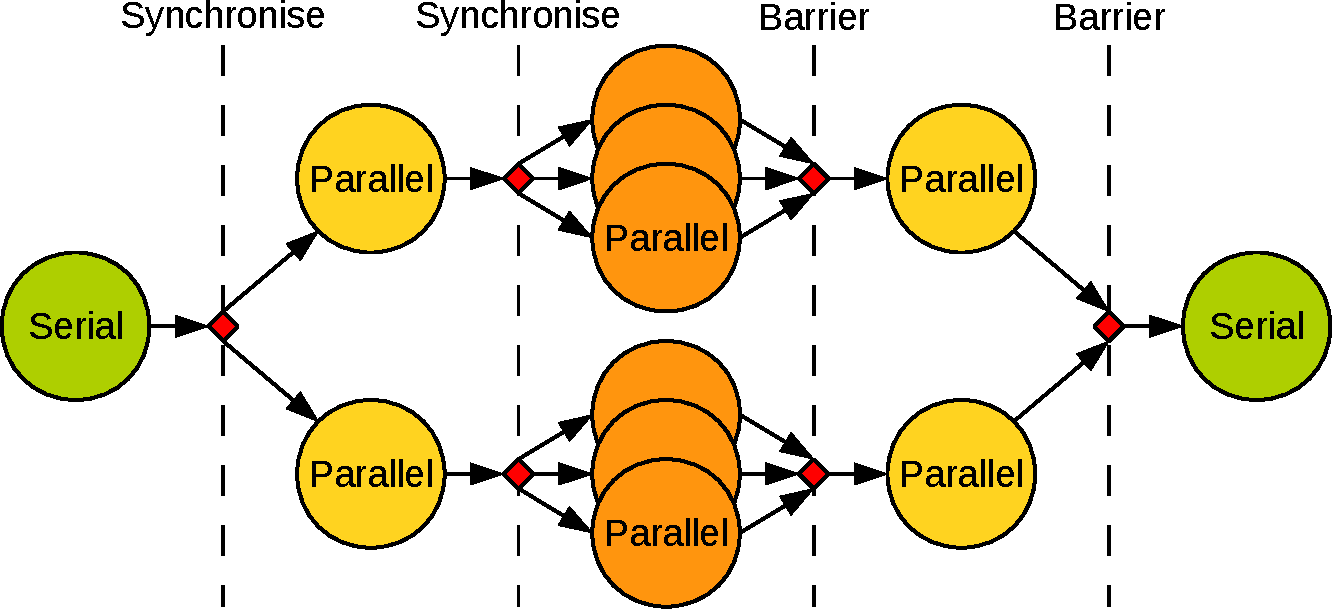
\includegraphics[width=\textwidth,height=\textheight,keepaspectratio]{software_sync}}
						\caption{Parallel software behaviour} 
						\label{software_sync}
				\end{figure}
				
				Figure \ref{software_sync} is a conceptual representation of generic parallel software behaviour \cite{Choi00_0,Choi00_1}. Most coherence schemes based on time, rely on this behaviour. The synchronisation and barrier points can be effectively exploited by the compiler or hardware to achieve global consistency; elaborated by Fensch \cite{Fensch08}.

				Hardware designs can be simplified through improved compiler support and better exploitation of data spacial and temporal locality. Such a design can provide coherence support to systems without hardware coherence, such as the Cray T3D processor, as demonstrated by Choi et al. \cite{Choi94,Choi96,Choi00_0,Choi00_1}. 
				Similar to TS, their coherence scheme associates timestamps with memory locations. However, their design relies on a special time-read instruction which checks memory location timestamps.
				This compiler inserted instruction, is aware of the most recent write to a memory location, and if the targeted memory location is older than the write, it is invalidated. 
				By the authors own description, this system mostly relies on correct compiler analysis. 
			
		
			\subsection{Hardware-Assisted Approach}
				There have been a number of proposals combining directory or snooping protocols with some form of timestamp coherence \cite{Lebeck95,Lai00,Yu15_0,Yu15_1,Kurian15}. These designs display an improvement over the base protocol and most of them enforce a strict memory consistency policy.

				In recent work by Elver and Nagarajan \cite{Elver14}, timestamps are added to memory locations as a means of reducing coherence communication overheads. Their scheme lowers the memory overheads of a MESI protocol by eliminating the sharing vector in shared memory, instead, the protocol tracks the current owner core. To compensate for an increase in coherence messages due to limited tracking, timestamps are added to the local and shared caches. 

				Further modification of directories using timestamps have been shown in \cite{Shim11,Choi11,Sung15}. Most of this work is based on MESI style directories for x86, and strong consistency models. 
				Another potential use for time-based coherence aimed at GPUs has been shown by Singh et al. \cite{Singh13,Singh14}. Traditionally, GPUs support little or no coherence. The authors have shown that self-invalidating GPU caches can improve overall performance. 

				A number of schemes based on Lamport \cite{Lamport78} vector clocks have also been explored. Keleher et al. \cite{Keleher94} have demonstrated vector clock style communication, lazy memory consistency, communicating over Ethernet. In order to achieve good performance their system is highly optimised to reduce memory coherence communication. A relaxed memory consistency design has allowed them to batch memory operations and reduce the impact of false sharing. 
				
				Lis and Shim \cite{Shim11,Lis11} have proposed the concept of Library Cache Coherence (LCC), which allows caches to check out data for a fixed amount of time. The scheme is based around a global clock which enforces sequential consistency (SC). Hardware support for strong memory consistency schemes such as SC is usually challenging and costly, however, an efficient implementation of this scheme is desirable. SC significantly reduces software complexity. 
				
				The LCC scheme removes the need for multicast or broadcast invalidations, typically required in directory-based schemes. LCC efficiency relies on an appropriate choice of data lending period, effectively a cache line time-out; a short lending period increases cache misses, and long time-outs cause delays as cores wait for lines to expire. 
				
			\subsection{BERI Time-Based Approach}
				The time-based scheme discussed in this dissertation avoids explicit cache coherence messages. 
				This scheme relies solely on cache self-invalidation, and correct use of software synchronisation and locking mechanisms. 
				The coherence model complies with a well defined relaxed memory consistency scheme (RMO{\large$^\star$}) \cite{SPARCInternational94}, thus, providing strong programmer assurances (discussed in Section \ref{section_rmo}).
				
				In contrast to other related designs discussed in this section, the BERI time-based coherence scheme is designed to function as a standalone system and does not require any changes to the operating system, compiler, or the ISA. I evaluate this model on a full system design in hardware, unlike the related work which is demonstrated predominantly using software simulations.
				
				Very few related designs have been verified against a memory consistency model, they mostly rely on the observed software interactions to determine the consistency behaviour. More crucially, I demonstrate that common operating systems and compilers already include the support for such a coherence and consistency design.

%\clearpage
\section{Memory Consistency}
	\label{background_consistency}
		
	A memory consistency model defines the behaviour of memory operations and provides programmer guarantees. A consistency model is generally more critical in multiprocessor systems where memory operations originate from different processing elements. Memory consistency is usually described through strictness of memory operations, strong consistency implies limited reordering of operations by the memory subsystem, a relaxed model offers more freedom in this respect. 
	
	Strong models are conceptually easier to understand, their behaviour is more predictable and may be sequential. Models such as Total Store Order (TSO) or Sequential Consistency (SC) require hardware support, but software support may be less complex. Relaxed consistency permits various non-chronological orderings of memory operations. Software design requires careful planning in order to support Relaxed Memory Order (RMO), while hardware support is reduced.

	Architectures such as x86 and its variants generally provide strong memory consistency such as TSO. As a result programmers are guaranteed that all store operations will commit in some fixed chronological order, and will be concurrently observable to the entire system. Maintaining this memory behaviour requires extensive hardware support, coordinating appropriate synchronisation messaging.
	
	Processor designs such ARM or PowerPC demonstrate a different approach to memory consistency design \cite{Sarkar11,Maranget12}. Both systems opt for a relaxed memory behaviour. Explicit synchronisation instructions are used to maintain a global memory order. Hardware complexity is reduced, since memory communication is not forced to follow a particular pattern. This memory behaviour relies on the fact that most software is written to run independently and merge at specific intervals; previously displayed in Figure \ref{software_sync}.

	
	\subsection{Memory Consistency Trace Format}
		\label{mem_format}
	
		I have used the AXE and CHERI Litmus model checkers developed by Matthew Naylor \cite{AXE_checker,CHERI_litmus} to evaluate the memory consistency behaviour of time-based and directory coherence. AXE is a trace checker, and BlueCheck \cite{bluecheck} is used to stimulate the memory subsystem with random inputs. The memory trace format used by the model checker is shown in Equation \ref{test_mem_trace_format}. It reports whether or not a given trace satisfies one of its supported memory models.
	
		\begin{equation}
			C_{id}: \ M[M_{addr}] \ \risingdotseq \ \mathbb{N}
		\label{test_mem_trace_format}	
		\end{equation}
		
		
		\begin{table}[!h]
		\begin{center}
		\begin{tabular}{|c|l|}
			\hline
			C$_{id}$: & Core/Thread ID \\
			\hline
			M[\ \ ] & Memory operation (SYNC is a variant) \\
			\hline
			M$_{addr}$ & Address of the memory operation \\
			\hline
			$\risingdotseq$ & Memory operation type \\
			& Load (==), Store (:=) \\
			\hline
			$\mathbb{N}$ & Natural number stored/loaded \\
			\hline
		\end{tabular}
		%\caption{}
		\label{test_mem_trace_format_legend}
		\end{center}
		\end{table}
	
	\subsection{Defining Memory Consistency}
		The memory consistency models evaluated by AXE are defined in this section.
		 %The model checking tool (AXE) analyses memory traces for a given memory architecture, the traces are evaluated and matched against a consistency model, described further.

		\subsubsection{Sequential Consistency} 
			This consistency model was defined by Lamport \cite{Lamport79}: ``The result of any execution is the same as if the operations of all processors were executed in some sequential order, and the operations of each individual processor appear in this sequence in the order specified by its program.''

		\subsubsection{Total Store Order}
			The Oracle{\tiny{$^{\textregistered}$}} information library \cite{Oracle15} defines this memory model as: ``TSO guarantees that the sequence in which store, flush, and atomic load-store instructions appear in memory for a given processor is identical to the sequence in which they were issued by the processor.''
			
			\captionsetup[table]{name=Trace}
			\begin{table}[!hb]
			\begin{center}
			\fontfamily{pcr}\selectfont
			\begin{tabular}{|l|l|}
				\hline
				\multicolumn{1}{|c|}{\textbf{TSO Trace}} & \multicolumn{1}{c|}{\textbf{MIPS Assembler}} \\
				Init (x==0, y==0) & Init addresses (x) and (y) \\
				\hline
				0: x := 1 & ``li r1, 1 ; sw r1, 0(x)'' \\
				\textbf{\textcolor{ForestGreen}{0: y == 0}} & lw r2, 0(y) \\
				1: y := 1 & ``li r1, 1 ; sw r1, 0(y)'' \\
				\textbf{\textcolor{ForestGreen}{1: x == 0}} & lw r2, 0(x) \\
				\hline
				\multicolumn{2}{|c|}{\textbf{\textcolor{ForestGreen}{Allowed}}} \\
				\hline
			\end{tabular}
			\caption[TSO consistency compliance]{TSO consistency compliance (\textit{Note: Instruction sequences for each core are listed in program order, however, the relative ordering between the two cores is variable})}
			\label{tso_compliance}
			\end{center} 
			\end{table}
			\captionsetup[table]{name=Table}
			
			\captionsetup[table]{name=Trace}
			\begin{table}[!hb]
			\begin{center}
			\fontfamily{pcr}\selectfont
			\begin{tabular}{|l|l|}
				\hline
				\multicolumn{1}{|c|}{\textbf{TSO Failure}} & \multicolumn{1}{c|}{\textbf{MIPS Assembler}} \\
				Init (x==0, y==0) & Init addresses (x) and (y) \\
				\hline
				0: x := 1 &  ``li r1, 1 ; sw r1, 0(x)'' \\
				0: sync & sync (barrier) \\
				\textbf{\textcolor{red}{0: y == 0}} & lw r2, 0(y) \\
				1: y := 1 & ``li r1, 1 ; sw r1, 0(y)'' \\
				1: sync & sync (barrier) \\
				\textbf{\textcolor{red}{1: x == 0}} & lw r2, 0(x) \\
				\hline
				\multicolumn{2}{|c|}{\textbf{\textcolor{red}{Disallowed}}} \\
				\hline
			\end{tabular}
			\caption{TSO consistency non-compliance}
			\label{tso_non_compliance}
			\end{center} 
			\end{table}
			\captionsetup[table]{name=Table}

			
			Trace \ref{tso_compliance} shows a memory ordering example satisfying TSO conditions. TSO permits the writes to \textbf{(x)} and \textbf{(y)} to be buffered locally at each hardware thread, allowing the subsequent loads of \textbf{(x)} and \textbf{(y)} to execute before the writes have reached shared memory. The loads to those addresses are permitted to observe initial values even after an update.

			Trace \ref{tso_non_compliance} shows TSO non-compliance. The synchronisation instructions force the writes to \textbf{(x)} and \textbf{(y)} to be flushed to shared memory before the subsequent loads of \textbf{(x)} and \textbf{(y)} can be performed. This example does not comply with any memory consistency model described in this dissertation.
			
		\subsubsection{Partial Store Order}
			The Oracle{\tiny{$^{\textregistered}$}} information library \cite{Oracle15} defines this memory model as: ``PSO does not guarantee that the sequence in which store, flush, and atomic load-store instructions appear in memory for a given processor is identical to the sequence in which they were issued by the processor. The processor can reorder the stores so that the sequence of stores to memory is not the same as the sequence of stores issued by the CPU.''
			
			Trace \ref{pso_compliance} shows a memory ordering scenario permitted by PSO. Both updates of \textbf{(x)} and \textbf{(y)} are performed by the same core, however, writes may be buffered and propagated in different orders. Thus, two load operations on another core may observe the memory values out-of-order.
			
			\captionsetup[table]{name=Trace}
			\begin{table}[!h]
			\begin{center}
			\fontfamily{pcr}\selectfont
			\begin{tabular}{|l|l|}
				\hline
				\multicolumn{1}{|c|}{\textbf{PSO Trace}} & \multicolumn{1}{c|}{\textbf{MIPS Assembler}} \\
				Init (x==0, y==0) & Init addresses (x) and (y) \\
				\hline
				0: x := 1 & ``li r1, 1 ; sw r1, 0(x)'' \\
				0: y := 1 & sw r1, 0(y) \\
				1: y == 1 & lw r1, 0(y) \\
				\textbf{\textcolor{ForestGreen}{1: x == 0}} & lw r2, 0(x) \\
				\hline
				\multicolumn{2}{|c|}{\textbf{\textcolor{ForestGreen}{Allowed}}} \\
				\hline
			\end{tabular}
			\caption{PSO consistency compliance}
			\label{pso_compliance}
			\end{center} 
			\end{table}
			\captionsetup[table]{name=Table}

		\subsubsection{Relaxed Memory Order}
			\label{section_rmo}
			This model further relaxes the rules on ordering of load and store operations; loads can be reordered with respect to other loads and stores to different addresses. Explicit synchronisation instructions are used to maintain a global order. Dependencies imposed by the memory subsystem can also affect the consistency model. 
			
			The SPARC--V9 architectural manual \cite{SPARCInternational94} states the following: ``Dependence order is a partial order that captures the constraints that hold between instructions that access the same processor register or memory location.'' Thus, two flavours of RMO exist, with and without dependencies. RMO with dependencies is a subset of RMO without dependencies. The PowerPC memory model falls somewhere in between the two, being stronger than RMO without dependencies but weaker than RMO with dependencies.

			\begin{figure}[t]
				\centering 
					\makebox{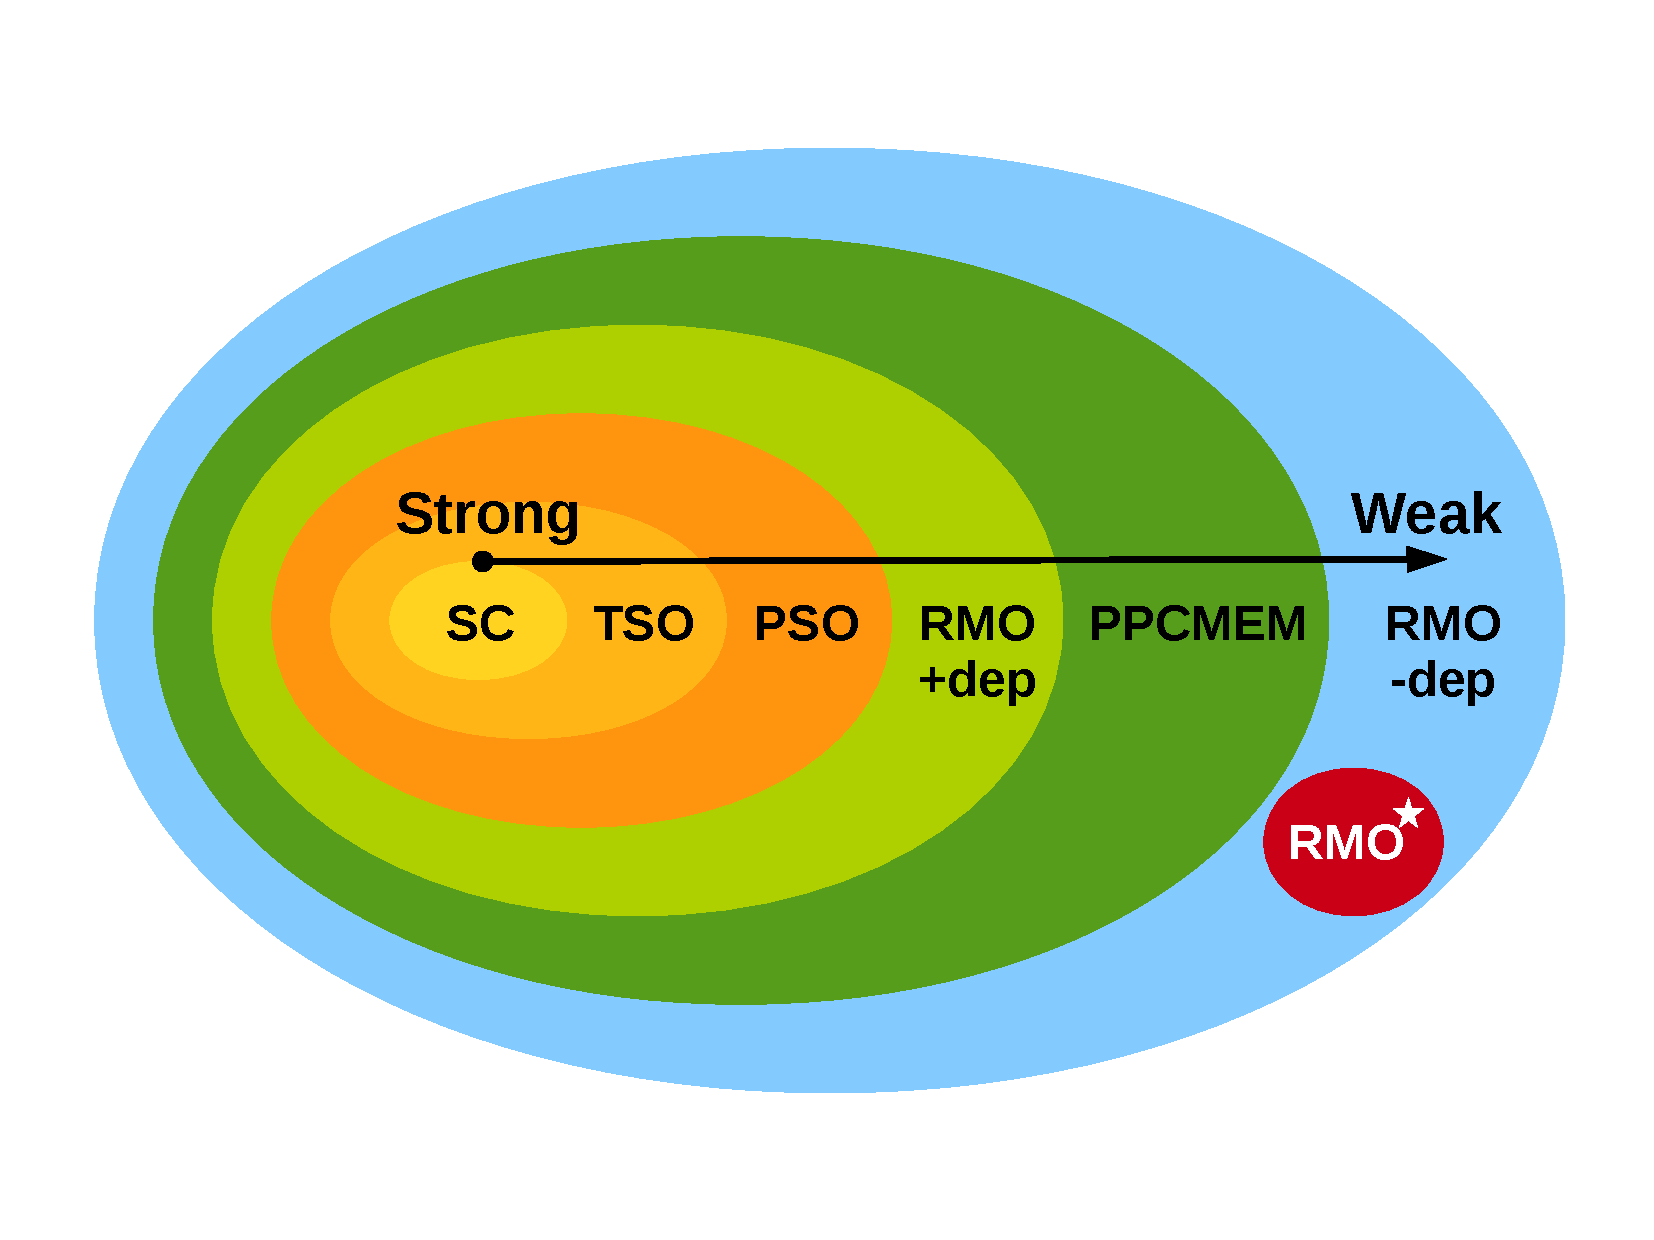
\includegraphics[trim={0 1.8cm 0 1.8cm},clip,width=0.75\textwidth,height=0.75\textheight,keepaspectratio]{consistency_sets}}
					\caption[Memory consistency model hierarchy]{Memory consistency model hierarchy. (\textit{Note: [+dep] and [--dep] indicate model evaluation with and without dependencies, respectively})} 
					\label{consistency_sets}
			\end{figure}
	
			\captionsetup[table]{name=Trace}
			\begin{table}[b]
			\begin{center}
			\fontfamily{pcr}\selectfont
			\begin{tabular}{|l|l|}
				\hline
				\multicolumn{1}{|c|}{\textbf{RMO Trace}} & \multicolumn{1}{c|}{\textbf{MIPS Assembler}} \\
				Init (x==0, y==0) & Init addresses (x) and (y) \\
				\hline
				0: x := 1 & ``li r1, 1 ; sw r1, 0(x)'' \\
				0: sync & sync (barrier) \\
				0: y := 1 & sw r1, 0(y) \\
				1: y == 1 & lw r1, 0(y) \\
				\textbf{\textcolor{ForestGreen}{1: x == 0}} & lw r2, 0(x) \\
				\hline
				\multicolumn{2}{|c|}{\textbf{\textcolor{ForestGreen}{Allowed}}} \\
				\hline
			\end{tabular}
			\caption{RMO consistency compliance}
			\label{rmo_compliance}
			\end{center} 
			\end{table}
			\captionsetup[table]{name=Table}
	
			The time-based coherence model described in this dissertation falls under RMO without dependencies, for convenience it will be referred to as \textbf{RMO{\large$^\star$}}. Figure \ref{consistency_sets} shows a hierarchy of memory consistency models based on strength, from strict to relaxed consistency. Examples of litmus tests shown in Chapter \ref{chapter_validation}, highlight the nuances in RMO{\large$^\star$} behaviour. 
			%The model has been checked with the complete AXE litmus test suite, as well as CHERI litmus tests. These tests have shown that RMO{\large$^\star$} falls under RMO without dependencies and does not violate any properties of this consistency model.
			
			Trace \ref{rmo_compliance} shows an example of RMO behaviour, the synchronisation instruction forces the writes to be performed in order, but now the loads can execute out-of-order, hence, this behaviour is allowed under RMO but not PSO. Core 1 does not perform any synchronisation operations, thus, both updated and stale values may be observed.
			
			\captionsetup[table]{name=Trace}
			\begin{table}[!h]
			\begin{center}
			\fontfamily{pcr}\selectfont
			\begin{tabular}{|l|l|}
				\hline
				\multicolumn{1}{|c|}{\textbf{RMO No Dependencies}} & \multicolumn{1}{c|}{\textbf{MIPS Assembler}} \\
				Init (x==0, y==0) & Init addresses (x) and (y) \\
				\hline
				0: x := 1 & ``li r1, 1 ; sw r1, 0(x)'' \\
				0: sync & sync (barrier) \\
				0: y := 1 & sw r1, 0(y) \\
				\textbf{\textcolor{BurntOrange}{1: y == 1 (block)}} & ``lw r1, 0(y) ; xor r3, r1, r1'' \\
				\textbf{\textcolor{ForestGreen}{1: x == 0}} & lw r2, \textbf{\textcolor{BurntOrange}{r3}}(x) \\
				\hline
				\multicolumn{2}{|c|}{\textbf{\textcolor{ForestGreen}{Allowed}}} \\
				\hline
			\end{tabular}
			\caption{RMO compliance, without dependencies}
			\label{rmo_no_dep_compliance}
			\end{center} 
			\end{table}
			\captionsetup[table]{name=Table}
			
			Trace \ref{rmo_no_dep_compliance} is an example of RMO compliance but only applicable when the memory subsystem does not block operations (without dependencies). If the system were to block the load of \textbf{(y)}, then only an updated value of \textbf{(x)} would be observed. This does not happen in RMO without dependencies (RMO{\large$^\star$}). 
			
			An advantage of a weak memory model is that it can be made stronger through synchronisation instructions, however, a strong model cannot be made weaker. It may be easier to design applications for strong models but the flexibility of weak models may be lost.

%\clearpage
\section{Cache Side-Channel Attacks}
	Contention for a hardware resource may cause unanticipated side-effects, for instance, system performance variation affect all sharers. These side-effects can expose the details of current users resource usage. The shared resource need not be a physical device. For example, information can be extracted from electromagnetic emanations, power analysis \cite{Mangard07}, or even audio analysis. Observations of side-effects with malicious intent are referred to as side-channel attacks (SCAs).
	
	In this dissertation I focus on timing cache SCAs, where the shared resource is a cache and the sharer maybe a thread, core, or another device. Useful information is usually extracted by measuring cache access latency. Latency increases with the increase in cache contention. Performance of a cache depends on its architectural structure and the applied workload. 
	
	Caches are typically designed to hide memory latency. Most caches will still provide some side-channel information, barring caches designed explicitly for side-channel mitigation \cite{Liu13}. The workload imposed on a cache can have a profound effect on side-channels. Higher single thread usage may provide greater leakage, whereas, multiple threads actively using the cache may mask each other.
	 
	SCAs on caches are summarised by Osvik et al. \cite{Osvik06}: ``Systems concurrently execute programs with different privileges. Kernel/userspace separation, process memory protection, system permissions, virtual machines, sandboxes, and other techniques are used to ensure desired access control semantics. The model is highly idealized and does not consider the intricacies of the actual implementation.	The processor and its infrastructure is a resource that all processes compete for, hence, processes will indirectly influence each other's behaviour. Data stored in a cache is protected by virtual memory mechanisms, however, the cache behaviour itself is exposed to a certain degree and can be profiled.''
	
	Cache timing attacks have become even more critical as emerging cloud computing services allow collocation of virtual machines (VM). This could allow an attacker to spy on other VMs and extract critical information. An example of this attack is demonstrated by Ristenpart et al. \cite{Ristenpart09}. A targeted attack may be difficult due to the uncertainties introduces by the cloud infrastructure, however, it might still be possible to extract commonly used keys or other secret information by observing VM behaviour.
	
	\subsection{Cryptography and SCAs}
		Research on SCAs predominantly focuses on breaking popular cryptographic algorithms. Attacks do not expose weakness in the cryptographic design itself, but instead use software characteristic of the algorithm to uncover the secret. Early SCA research focused on obtaining keys to cryptographic algorithms such as: Diffie-Hellman, RSA, DSS, DES, and OpenSSL \cite{Kocher96,Tsunoo03,Kelsey98,Brumley03}. 
		
		More recently, AES has been the primary target for SCAs \cite{Bernstein05,Percival05,Osvik06,Bonneau06_0,Bonneau06_1}. The algorithms mentioned above, perform multiple cryptographic rounds on plain text using the key. Each cryptographic round will use some memory through table lookups, modular exponentiation \cite{Kocher96}, etc. In the case of AES, memory usage is directly associated with the combination of plain text and the key, different values will produce variable memory usage during the cryptographic rounds. 
	
		Understanding a cryptographic scheme plays a critical role in deciphering any side-channel timing data. Early research shown by Hu \cite{Hu92} suggested a strong method of performing an SCA through separate Trojan and spy applications. In this scenario the Trojan holds a higher OS privilege than the spy. The main aim of the Trojan is to gather cache timing information and then pass it on to the spy who will either analyse and/or forward this data to a remote system. The Trojan application attempts to measure cache hits/misses by timing accesses to its own cached data. 
		
		The attack begins with the Trojan loading its data into the cache. A critical application, referred to as the Victim, is launched by the scheduler once the Trojan operation is complete. The Victim algorithm uses the cache to store its own private data, thus evicting some of the Trojan data (we assume no other software interferences in this example). Once the Victim operation is complete, the Trojan reads back its data and measures the access latency. 
		
		Cache misses will take longer than hits, and this information is sufficient to identify memory locations used by the Victim. The spy can then analyse this timing data and extract Victims secret information, such as the cryptographic key. This attack is often referred to as Prime+Probe \cite{Osvik06}. Other attacks often rely on the specific behaviour of a cryptographic algorithm, attacks on individual rounds are one such example.
		
		The attacker must be aware of various architectural features of the target system in order to conduct a successful SCA. If the attacker is able to replicate and profile the target system, it may be much easier to conduct an SCA. Template attacks are one such example. The attacker captures cache timing information from the target system and then evaluates the data against the replica. Such attacks can be highly covert, recovering the full cryptographic key with only 800 target samples. The overall measurement time may be as low as 65ms, followed by 3 sec of analysis on the replica \cite{Brumley09,Osvik06}. Knowing the cache profile allows the attacker to conduct this attack without any knowledge of ciphertext or plaintext. 
		
		In this dissertation I attempt to quantify side-channel leakage of a given cache hierarchy and then investigate if a cache coherence scheme has any effect on leakage. The analysis does not focus on any specific cryptographic algorithm, instead I use common SCA techniques to perform controlled tests against simple applications. The Trojan application attempts to determine the memory usage of a Victim and ultimately profile the cache behaviour.

	\subsection{SCA Mitigation}
		Early SCA analysis on the VAX security kernel was documented by Hu \cite{Hu91,Hu92}, suggesting several ways of mitigating Prime+Probe attacks:
		\begin{enumerate}
			\item Clearing the cache/caches when context switching (costly due to processor stalls).
			\item Using ``fuzzy time''.
			\item A custom scheduler that is aware of security critical applications.
		\end{enumerate}
		Cache flushing provides some side-channels mitigation, however, it may require many cycles to complete and could evict valid data. The notion of ``fuzzy time'' supports the concept of eroding side-channel leakage through time-based cache self-invalidation. The example described in the paper focuses on mitigating SCAs on RAM through variations in clock rates. 
		The time-based model follows a similar principle of adding timing entropy through self-invalidation, reducing the risk of leaking useful timing information through side-channels.
		In principle cache self-invalidation is similar to cache flushing, but only requires a single instruction to complete.
	
		Various other SCA masking and mitigation techniques have been evaluated in the past, the effective methods have been summarised by Osvik and Tromer \cite{Osvik06,Tromer10}. Most techniques are applied to a specific cryptographic algorithm but some are more general. 
		
		\paragraph{General Techniques}
			\begin{enumerate}
			\item Tuning all memory access pattern to behave in a similar way, regardless of cache performance. 
			\item The ``fuzzy time'' technique. However, it may be circumvented by acquiring more timing samples, as demonstrated by Bonneau \cite{Bonneau06_0} and Tiri et al. \cite{Tiri07}.
			\item Normalising the cache state by evicting all Victim data.
			\item Cache partitioning, Wang and Lee \cite{Wang07}.
			\item Disabling cache sharing.
			\item Completely disabling the cache. Some Intel processors allow privileged cache accesses and ARM models provide a lockable mini-cache. Both methods have some drawbacks, such as the cost of cache enabling and disabling, as well as cache size limitations.
			\item Dynamic cache remapping and eviction randomization, Liu and Lee \cite{Liu13}.
			\item Explicit OS support through scheduling considerations.
			\end{enumerate}
		
		\paragraph{AES Specific Techniques}
			\begin{enumerate}
			\item Replacing table lookups with an equivalent series of logical operations.
			%\item Avoiding lookup tables or pre-loading AES tables.
			\item Architectures with large register files can hold an entire s-box table.
			\item Full or random cache warming by loading the entire s-box table and avoiding misses, Page \cite{Page02,Page05}.
			\item Modifying the implementation of AES to use smaller table sizes, Brickell et al. \cite{Brickell06}. Cache leakage will be restricted to a cache line granularity and smaller tables will reduce attack accuracy.
			\item Dynamic table storage. Multiple s-boxes are placed throughout memory and then accessed pseudo randomly.
			\item Selective round protection. Particularly vulnerable rounds can be speed up through one of the mentioned techniques mentioned previously.
			\end{enumerate}

\section{Summary}
	In this chapter I have examined various cache coherence techniques and highlighted their drawbacks. I propose the time-based coherence model which requires no additional software and simplifies the hardware design. Memory consistency is an important part of cache coherence and relaxed memory order supported by time-based coherence offers software and hardware flexibility.
	
	Cache side-channel mitigation techniques are typically limited to software masking or dedicated hardware solutions. I propose using time-based coherence as an inbuilt SCA masking mechanism. This coherence scheme provides correct multiprocessor system behaviour while also offering some SCA mitigation.


















































\begin{comment}
		List of citations:
		\begin{enumerate}
			\item \cite{Chaiken90}: One of the first papers in field.
			\item \cite{Agarwal88}: One of the first papers in field. Shows benefits of directory scaling, also mentions that snooping is popular
			\item \cite{Stenstrom90}: Large survey, includes snooping, directories and software schemes
			\item \cite{Lilja93}: Comparison of large scale shared mem procs issues, many designs discussed here. coherence detection and enforcement strategy. Improving memory utilization in cache coherence directories. The authors present two compiler optimizations that exploit the high-level sharing information available to the compiler to further reduce the size of a tagged directory by allocating pointers only when necessary.
			\item \cite{Martin03}: Token coherence. novel approach
			\item \cite{Byrd99}: Producer consumer relationship evaluation
			\item \cite{Lawrence98}: Another comprehensive coherence survey
			\item \cite{Marty08} various techniques including snooping, directory and token
			\item \cite{Adve96}: sequential mem consistency --- relaxed mem consistency
			\item \cite{Leverich07}: There are two basic models for the on-chip memory in CMP systems:hardware-managed coherent caches and software-managed streaming memory. This paper performs a direct comparison of the two models under the same set of assumptions about technology, area, and computational capabilities.
			\item \cite{Martin12}: Directory scalability. This paper refutes this conventional wisdom by showing one way to scale on-chip cache coherence with bounded costs by combining known techniques such as: shared caches augmented to track cached copies, explicit cache eviction notifications, and hierarchical design.
			\item \cite{Lenoski92}: The Stanford DASH, basics of directory coherence
			\item \cite{Hammond00}: The Stanford Hydra, CMP processor
			\item \cite{Chen91}: Comparison and Analysis of Software and Directory Coherence Schemes 
			\item \cite{Sanchez12}: SCD: A scalable coherence directory with flexible sharer set encoding
			\item \cite{Cuesta11}: Increasing the effectiveness of directory caches by deactivating coherence for private memory blocks. Talks about directory optimisations and analysing software usage of sharing
			\item \cite{James90}: Distributed-directory scheme: scalable coherent interface
			\item \cite{Cuesta13}: Increasing the Effectiveness of Directory Caches by Avoiding the Tracking of Noncoherent Memory Blocks
		\end{enumerate}
\end{comment}

\begin{comment}
	Related research on time-based coherence can be grouped under several main objectives and designs.
	\begin{enumerate}
	\item Compiler-directed coherence: 
		\begin{itemize}
		\item \cite{Cheong88}: TLB page tracking updates time-counter, penalty for TLB flushes. Write policies of caches are highlighted, write-back makes things difficult.
		\item \cite{Hoichi90}: Expands on the work above but also highlights problems with directory and large scale shared memory systems.
		\item \cite{Gutierrez12}: Using TLB directed cache invalidates for JIT compiled code.
		
		\item \cite{Choi94}: Per Epoch timestamps, requires a modified memory instruction, uses 4bit timestamps, claiming that is sufficient. The have an overflow mechanism so a full cache flush is unnecessary. A time-read to check for a potentially stale access, triggers a cache miss if invalid. (My system handles this internally). They use a fast counter just like in my system. ``Relies mostly on compiler analysis''
		\item \cite{Choi96}: Based on one above and implemented as below.
		\item \cite{Choi00_0}\cite{Choi00_1}: The previous version is tested on a Cray T3D computer and shown to outperform directory coherence in many cases. moves between epoch where each epoch can be serial or parallel. behaves much like pthread create and join. Uses weak consistency. ``Relies mostly on compiler analysis'' ``viable alternative for machines without hardware-coherent caches, such as the CrayT3D.'' My system does rely on compiler support but can also function if polling accesses or other synchronisation techniques are used, albeit that might be slow.
		\item \cite{Choi11}: Good support that modern software is good and better and faster memory systems can be designed. Showing better performance than MESI.
		\item \cite{Sung15}: proposes reader initiated sync's instead of just writer initiated sysncs. Acknowledges the limitations in current sync schemes and the need for finer granularity. writes are visible to all cores, writes are serialised. uses backoff counter to limit races. ``We assume the following software properties, which are already enforced by most modern programming languages: (1) Software obeys the standard data-race-free memory model adopted by C++, Java, and other languages [9, 26] that define sequentially consistent semantics for data-race-free programs. (2) Software distinguishes between synchronization and data accesses (also part of the requirement of data-racefree).''

		\item \cite{Darnell93}: TS,TC - PhD on the topic.
		\item \cite{Min92}: TS,TC - Trying to circumvent shared bus/memory architectures to provide limitless scaling. Clocks are assigned to each shareable data structure.
		\item \cite{Xin96} TS,TC 
		\end{itemize}
	\item Directory enhancement through timestamps:
		\begin{enumerate}
		\item \cite{Lebeck95}: attempting to implement dynamic self-invalidation for sequentially consistent systems. highlights that it is especially difficult to achieve for DSI. DSI significantly improves Directory when using SC, also improves it slightly under weak consistency, but only one benchmark.
		\item \cite{Lai00}: Uses DSI to pre-empt blocks in need of self-invalidation. Improves overall execution time.
		\item \cite{Elver14}: Self-Inv for TSO on x86. 
		\end{enumerate}
	\item SC - Lamport clock designs:
		\begin{enumerate}
		\item \cite{Keleher94}
		\item \cite{Shim11} 
		\item \cite{Lis11}
		\item \cite{Yu15_0}\cite{Yu15_1}\cite{Kurian15}\cite{Shim11}: Tardis
		\end{enumerate}
	\item For GPU's
		\begin{enumerate}
		\item \cite{Singh13}\cite{Singh14}
		\end{enumerate}
	\end{enumerate}
\end{comment}






\begin{comment}
This is TSO but not SC:
         li r1, 1
0: x := 1         sw r1, 0(x)
0: y == 0         lw r2, 0(y)
         li r1, 1
1: y := 1         sw r1, 0(y)
1: x == 0         lw r2, 0(x)
         assert (0:r2=0 and 1:r2=0)
\end{comment}


\begin{comment}
			This is TSO but not SC:
			
			0: x := 1
			0: y == 0
			1: y := 1
			1: x == 0
			
			This is not TSO:
			
			0: x := 1
			0: sync
			0: y == 0
			1: y := 1
			1: sync
			1: x == 0
\end{comment}

\begin{comment}
			This is PSO but not TSO:
			
			0: x := 1
			0: y := 1
			1: y == 1
			1: x == 0
\end{comment}

\begin{comment}
			This is RMO but not PSO:
			
			0: x := 1
			0: sync
			0: y := 1
			1: y == 1
			1: x == 0
			
			This is not RMO with deps:
			
			0: x := 1
			0: sync
			0: y := 1
			1: y == 1 (blocking)
			1: x == 0
\end{comment}

\begin{comment}

			\paragraph{Read-Consistency} 
				All memory models described in this thesis are read-consistent, whether weak or strong. If a model behaviour is proven to be non-read-consistent, then it does not satisfy any of the memory models described. 
				
				A given memory trace is read-consistent only if one the conditions listed below is satisfied. For a given program order \textbf{\textit{po}}, load \textbf{\textit{l}} of value \textbf{\textit{v}} from an address \textbf{\textit{a}} on thread \textbf{\textit{t}}:
				\begin{itemize}
					\item The last store to \textbf{\textit{a}} preceding \textbf{\textit{l}} in \textbf{\textit{po}} writes \textbf{\textit{v}}
					\item A store to \textbf{\textit{a}} with value \textbf{\textit{v}} is performed by a thread other than \textbf{\textit{t}}
					\item Address \textbf{\textit{a}} contains the initial value (\textbf{\textit{v} = 0})
				\end{itemize}

				In accordance with the quote, we specify the following constraint on memory operations: two instructions \textbf{\textit{i}} and \textbf{\textit{j}} executed by \textbf{\textit{t}} in \textbf{\textit{po}} must follow (\textbf{\textit{i}}$<$\textbf{\textit{j}}).

				\begin{itemize}
					\item If \textbf{\textit{i}} is a load then (\textbf{\textit{i}}$<$\textbf{\textit{j}})
					\item If both \textbf{\textit{i}} and \textbf{\textit{j}} are stores to the same or independent addresses then (\textbf{\textit{i}}$<$\textbf{\textit{j}})
					\item If either \textbf{\textit{i}} or \textbf{\textit{j}} are SYNC operations then (\textbf{\textit{i}}$<$\textbf{\textit{j}})
				\end{itemize}

				\begin{itemize}
					\item If \textbf{\textit{i}} is a load then (\textbf{\textit{i}}$<$\textbf{\textit{j}})
					\item If both \textbf{\textit{i}} and \textbf{\textit{j}} are stores to \textbf{\textit{a}} then (\textbf{\textit{i}}$<$\textbf{\textit{j}})
					\item If either \textbf{\textit{i}} or \textbf{\textit{j}} are SYNC operations then (\textbf{\textit{i}}$<$\textbf{\textit{j}})
				\end{itemize}

				\begin{itemize}
					\item If \textbf{\textit{i}} is a load to \textbf{\textit{a}} and \textbf{\textit{j}} is a store to \textbf{\textit{a}} then (\textbf{\textit{i}}$<$\textbf{\textit{j}})
					\item If both \textbf{\textit{i}} and \textbf{\textit{j}} are stores to \textbf{\textit{a}} then (\textbf{\textit{i}}$<$\textbf{\textit{j}})
					\item If either \textbf{\textit{i}} or \textbf{\textit{j}} are SYNC operations then (\textbf{\textit{i}}$<$\textbf{\textit{j}})
					\item If \textbf{\textit{i}} is a blocking operation then (\textbf{\textit{i}}$<$\textbf{\textit{j}})
				\end{itemize}
\end{comment}

% 3 lines below ensure that there is a blank page before a new chapter
\clearpage
\thispagestyle{empty}
\mbox{}
%TODO: Methods
\makeatletter
%\newcommand{\rmnum}[1]{\romannumeral #1 }
%\newcommand{\Rmnum}[1]{\expandafter\@slowromancap\romannumeral #1@}
\makeatother
\ifpdf
\graphicspath{{Chapter3/Chapter3Figs/PNG/}{Chapter3/Chapter3Figs/PDF/}{Chapter3/Chapter3Figs/}}
\else
\graphicspath{{Chapter3/Chapter3Figs/EPS/}{Chapter3/Chapter3Figs/}}
\fi

\chapter{BERI Multiprocessor Architecture}
	\label{chapter_methadology}

\section{BERI Architecture}
	The Bluespec Extensible RISC Implementation (BERI) processor is based on a 64-bit MIPS ISA. The processor is implemented in Bluespec SystemVerilog. The initial implementation was done by Gregory Chadwick \cite{Chadwick12,Chadwick13} and extended to support MIPS R4000 \cite{MIPS} by Jonathan Woodruff \cite{jon_thesis} and others \cite{BERITech_0,BERITech_1}.
	
	This processor has been developed as part of the CTSRD \& MRC2 projects \cite{CTSRD,MRC2}, hence, it is a good base platform for multiprocessor research and development. The team is also actively advancing the testing environment, model checking tools, compiler support and the operating system; ideal for hardware development and evaluation.
	
	BERI is a single issue, in-order processor with 6 pipeline stages. It has a branch predictor and register renaming. The memory structure consists of level 1 (L1) instruction and data caches, and a shared level 2 (L2) cache. 
	BERI with capability support is known as Capability Hardware Enhanced RISC Instructions (CHERI) \cite{Woodruff14,Watson12,Watson15}. 
	Figure \ref{beri_pipeline} shows a logical layout of the processor pipeline, control logic, and memory subsystem. 
	All variations of this processor can be synthesised to run on a Field Programmable Gate Array (FPGA) device.
	

	
	\paragraph{Pipeline Stages}	
		\begin{enumerate}
			\item Instruction Fetch: The program counter is used to request an instruction from memory.
			\item Scheduler: This stage is an optimisation, designed to access the register file and the branch predictor. 
			\item Decode: Instruction behaviour is identified.
			\item Execute: Arithmetic or assignment operations are performed at this stage.
			\item Memory Access: This pipeline stage communicates with memory through the data cache.
			\item Writeback: Any updates to the overall state are committed.
		\end{enumerate}

	\begin{figure}[t]
		\centering 
			\makebox{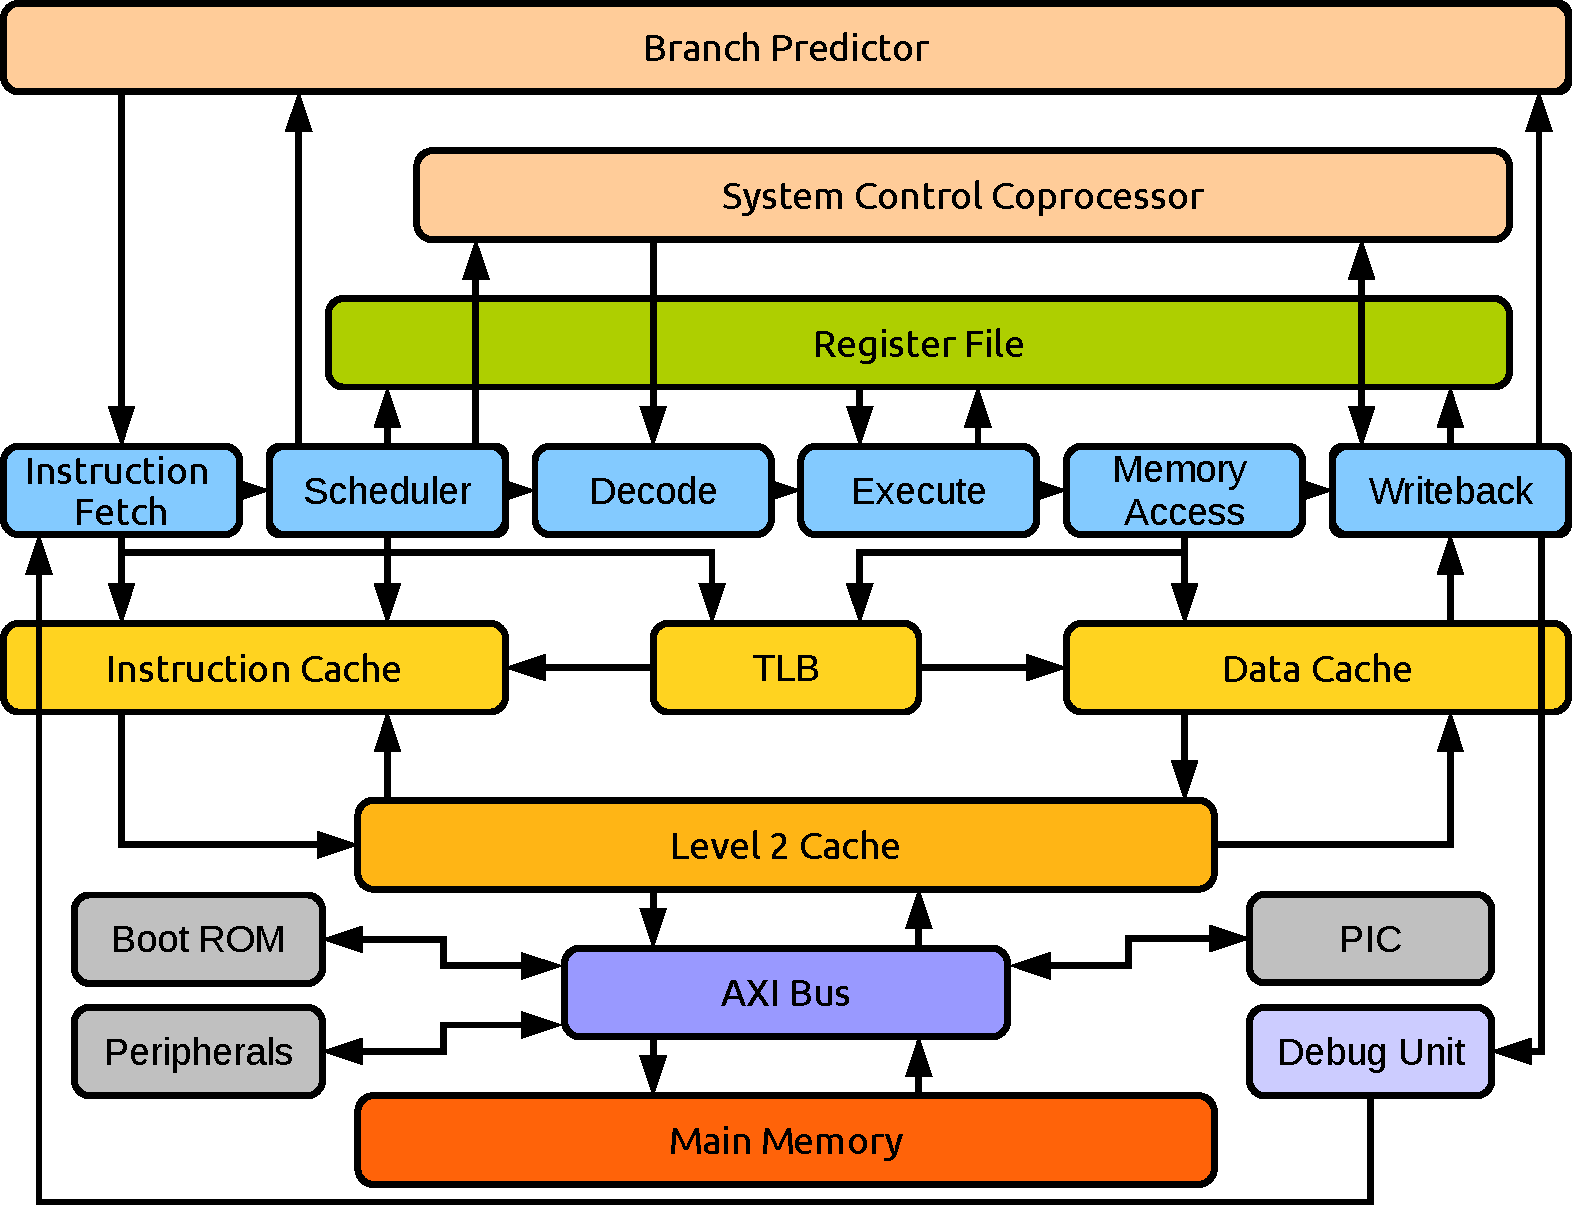
\includegraphics[width=0.97\textwidth,height=\textheight,keepaspectratio]{BERI_pipeline}}
			\caption{BERI processor architecture} 
			\label{beri_pipeline}
	\end{figure}

	\paragraph{Memory System}
		\begin{itemize}
			\item Instruction Cache: This L1 cache is designed to hold instructions and only performs loads.
			\item Data Cache: This L1 cache loads and stores data.
			\item L2 Cache: A shared cache responsible for holding both instructions and data.
			\item AXI Bus: A standard memory communication interface.
		\end{itemize}
		
	\paragraph{Peripherals}
		\begin{itemize}
			\item Boot ROM: Holds the memory contents required to boot the processor.
			\item Debug Unit: This device is used to inject instructions into the processor pipeline. The instructions can modify general purpose registers and memory. 
			\item PIC: The Programmable Interrupt Controller (PIC) multiplexes external interrupts.
		\end{itemize}
	
\section{Bluespec System Verilog}
	Traditional hardware description languages such as System Verilog have been widely used for hardware development. To aid productivity our research team has been exploiting a higher-level HDL, Bluespec System Verilog (BSV) \cite{bluespec,richards10} is a language initially developed at the Massachusetts Institute of Technology that allows extensible hardware design development. It is currently a property of Bluespec Inc. \cite{BSVREF}. 
	
	BSV adds a much needed level of abstraction to System Verilog, a rich type system, and flow control. The BSV language, together with the BSC compiler generate synthesisable Verilog RTL or SystemC. BSV retains some of the structure and syntax of System Verilog but also adds some Haskell syntax, improving the language extensibility.
	
	Bluespec designs synthesised into SystemC can be simulated using Bluesim to produce a cycle accurate model. Some tests and results presented in this dissertation are based on Bluesim output. The simulator has proven to be an excellent tool for testing and debugging our processor designs. Additionally, the produced results closely match hardware behaviour, making it an invaluable tool.

\section{Multiprocessor BERI Design}
	I have extended the BERI processor core into a multi-core design. Multi-core BERI supports a large number of cores; the design complexity and size is limited by the Bluespec compiler synthesis time, FPGA area, and the shared memory design. Most of the work described in this dissertation is based on a dual-core BERI, however multi-core version with up to 12 cores have been tested in simulation. Due to FPGA size limitations, the hardware tests have been limited to 1-4 cores on Altera DE-4 Stratix-4 \cite{TerasicDE4}; larger FPGAs should be able to support more cores.

	BERI multi-core is a shared memory multiprocessor. The private L1 caches of each BERI core (I-Cache and D-Cache) communicate with a single shared L2 cache. Numerous pipeline modifications were made in order to support multiple cores. The performance of larger designs will be limited by the shared L2 cache and communication interfaces. Several memory coherence models have been tested as a part of this research, I discuss two in this dissertation, directory coherence and time-based coherence, justified in Chapter \ref{chapter_background}. 
	
	\subsection{Memory Modification}
		\paragraph{Directory Coherence} The directory is contained within the L2 cache (Figure \ref{beri_directory}). If the directory identifies memory sharing and chooses to invalidate a privately cached line, it sends a message through a dedicated coherence interface. The message is processed by a coherence module which selects recipients based on the list of sharers. This ensures no coherence congestion on the shared bus and fast invalidate delivery. 
		
		\begin{figure}[t]
			\centering 
				\makebox{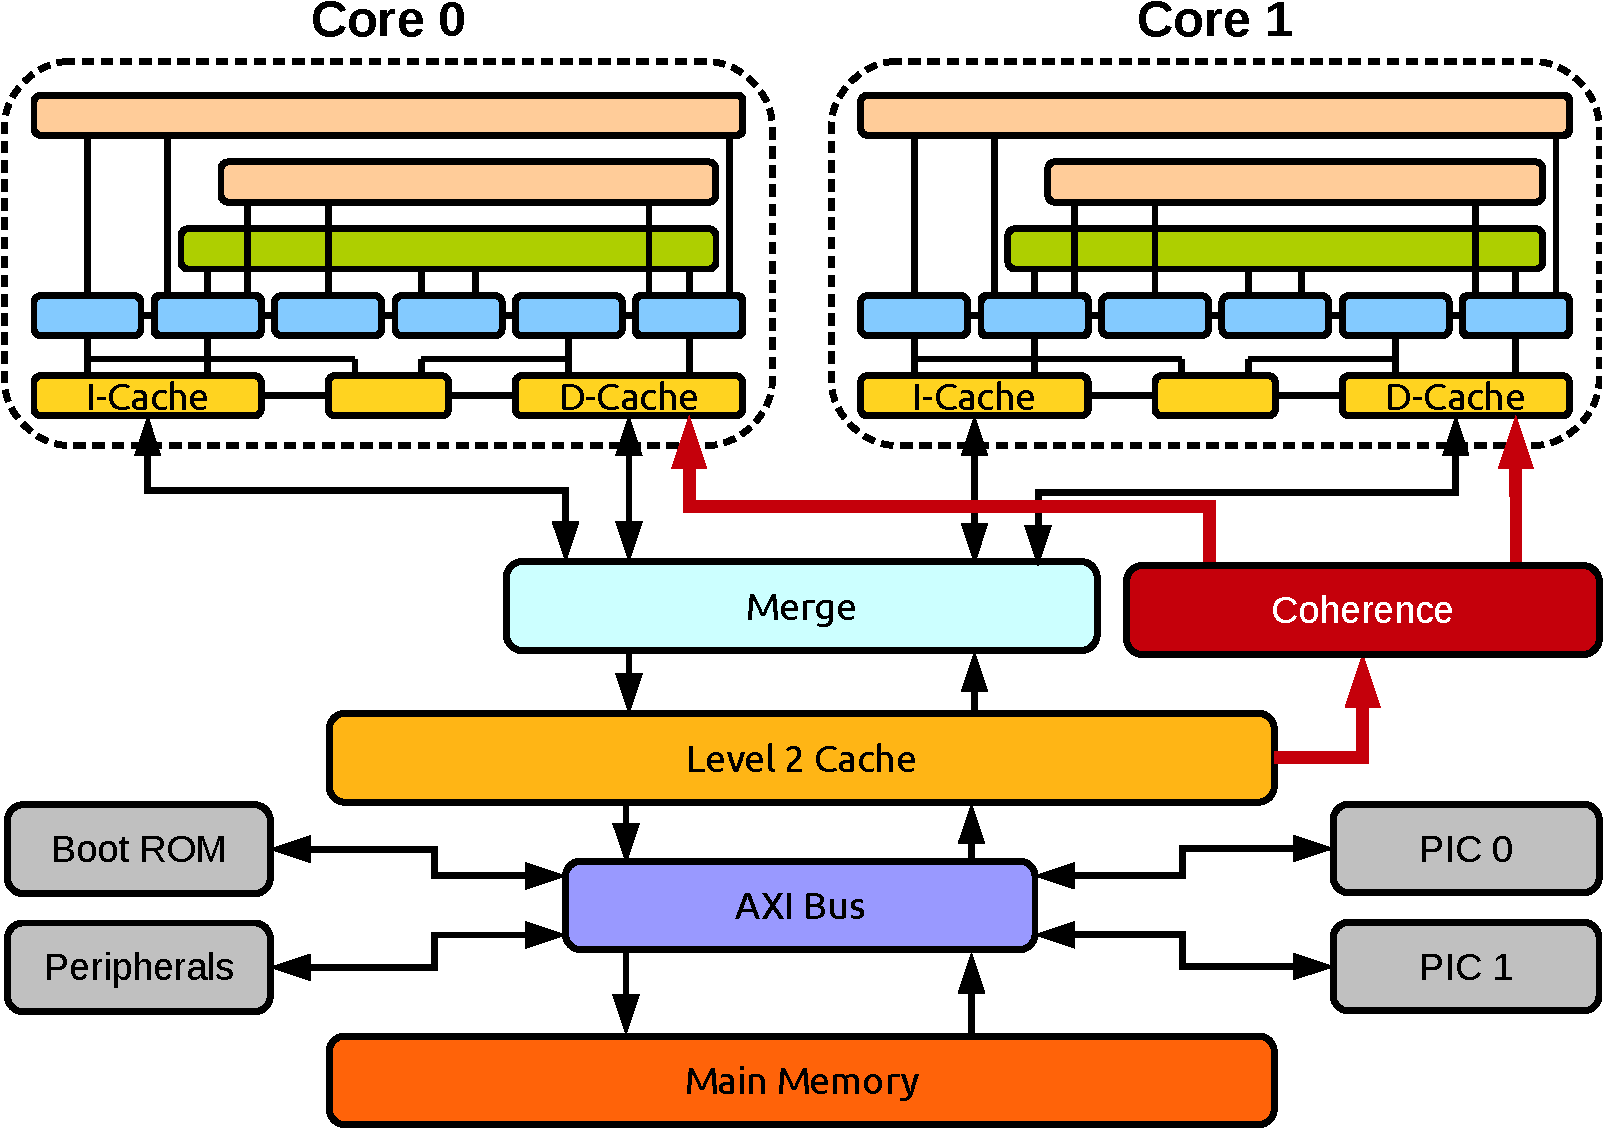
\includegraphics[width=\textwidth,height=\textheight,keepaspectratio]{BERI_directory}}
				\caption{BERI dual-core processor, directory-based coherence} 
				\label{beri_directory}
		\end{figure}
		
		\paragraph{Time-Based Coherence} This coherence scheme operates from within the private caches, performing self-invalidation (Figure \ref{beri_timebased}). As a result, the L2 cache is stock and no coherence module or network is required.
		
		\begin{figure}[t]
			\centering 
				\makebox{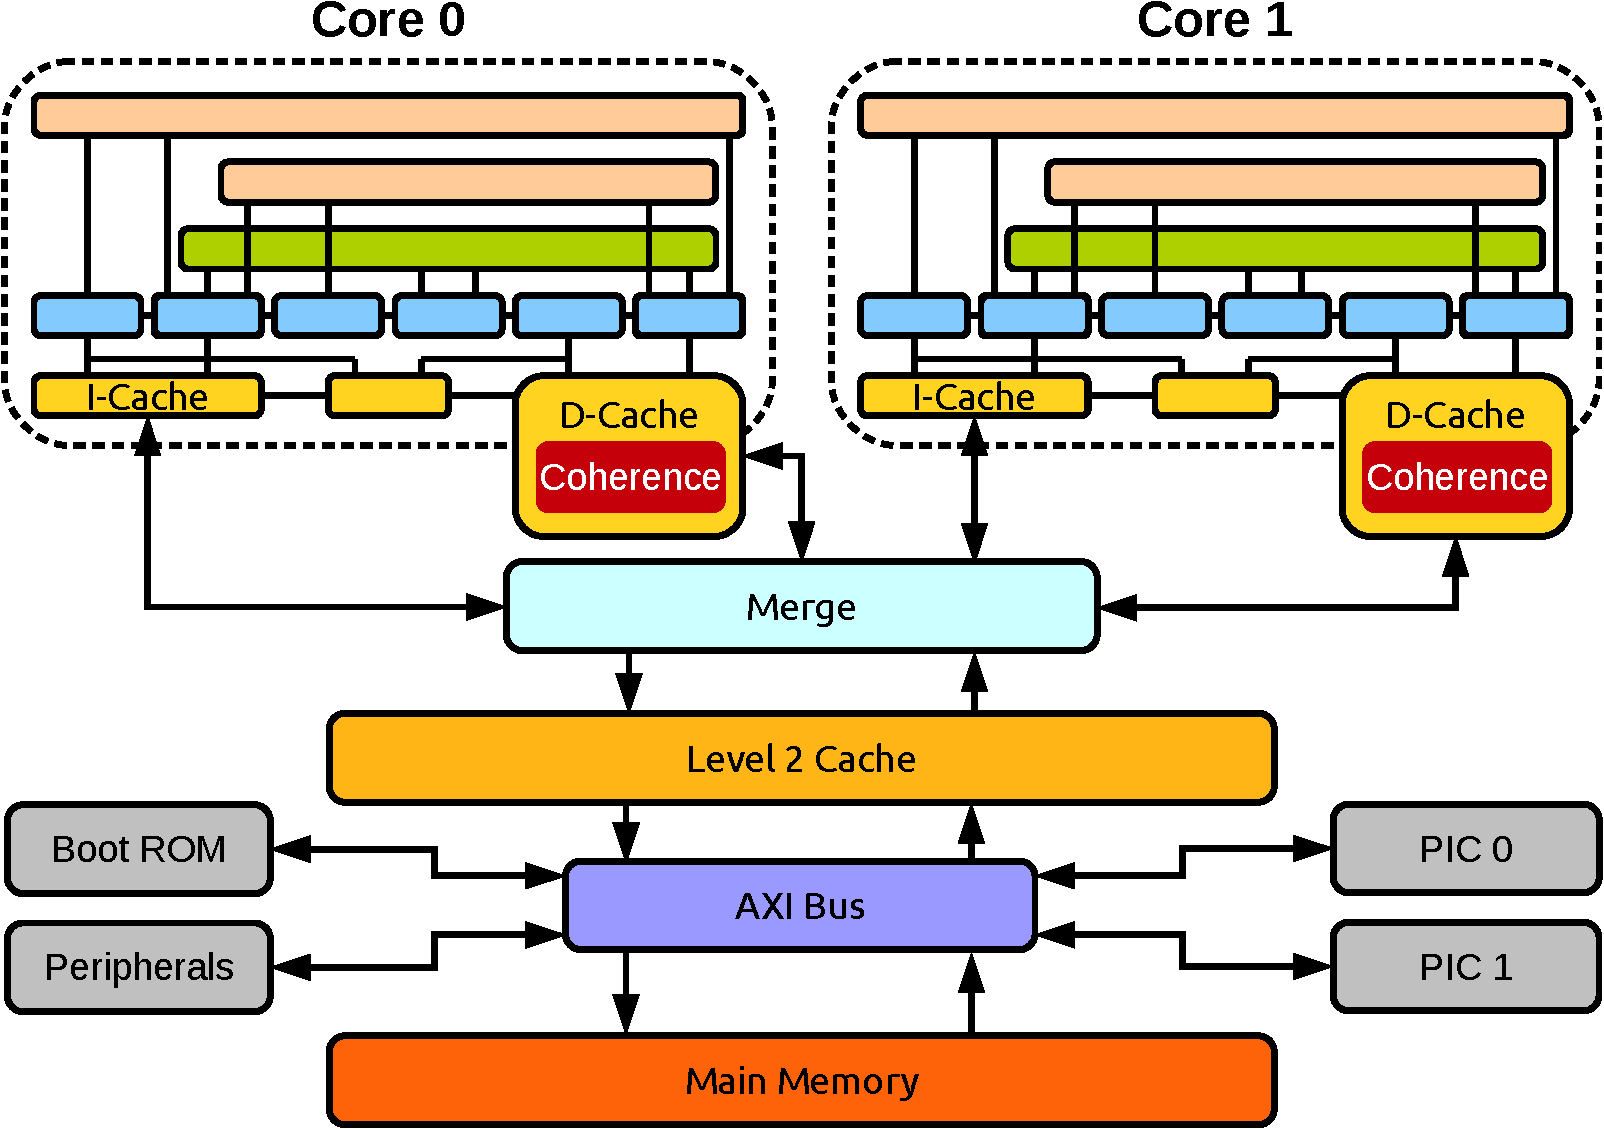
\includegraphics[width=\textwidth,height=\textheight,keepaspectratio]{BERI_timebased}}
				\caption{BERI dual-core processor, time-based coherence}
				\label{beri_timebased}
		\end{figure}


	\subsection{Core Identification}
		Software often requires a method for identifying individual processor cores. The operating system learns the hardware set up and uses this information to schedule software threads. Core identification is accomplished though a special coprocessor 0 (CP0) instruction. The mechanism used in BERI is similar to MIPS processors \cite{MIPS}. The ID is accessible in kernel-space and returns a 32 bit value. The bottom 16 bits hold the core id and the top 16 bits contain the total core count \{0 = One Core\}.
		%(Figure \ref{core_id}). 
		The distribution of core identifiers occurs at Bluespec compile time. Once built, the identifiers are fixed and cannot be changed or overwritten. 
		%This register is accessed during the FreeBSD boot procedure.

		\begin{comment}
		\begin{figure}[!h]
		\centering
			\newcommand{\colorbitbox}[3]{%
			\rlap{\bitbox{#2}{\color{#1}\rule{\width}{\height}}}%
			\bitbox{#2}{#3}}
			\definecolor{lightcyan}{rgb}{0.6,1,1}
			\definecolor{lightgreen}{rgb}{0.7,1,0.7}
			\begin{bytefield}[bitheight=\widthof{~Valid~},bitwidth=\widthof{\large x~},
			boxformatting={\centering\small}]{32}
			\bitheader[endianness=big]{31,16,15,0} \\
			\colorbitbox{lightgreen}{16}{Total Core Count} &
			\colorbitbox{lightcyan}{16}{Individual Core ID} &
			\end{bytefield}
			\caption{BERI Core Identification} 
			\label{core_id}
		\end{figure}
		%\vspace{-5mm}
		\end{comment}
		
	\subsection{Interrupt Delivery}
		In commercial multiprocessors, interrupts are often serviced through a hierarchy of programmable interrupt controllers (PIC's). The master PIC distributes interrupts to PIC's further down the hierarchy. The original PIC for single-core BERI was developed by Robert Norton \cite{Norton15}. BERI multi-core requires one PIC per core. The hierarchy is flat and interrupts are delivered to the PIC's simultaneously. Individual PIC's decide whether an interrupt should be reported to the given core.

	\subsection{Load Linked and Store Conditional}
		The correct implementation of synchronisation Load-Linked (LL) and Store Conditional (SC) instructions is critical for correct multiprocessor operation.
		The pair of instructions is frequently used in multithreading to achieve synchronisation. LL acts much like a typical load instruction and returns data from memory, an SC to the same memory location will only store data if no other updates have occurred since the LL. The SC instruction is expected to return a response, success or failure. 
		
		The behaviour of LL and SC operations is implementation and ISA dependent. The constrained ISA specification can be exploited by hardware designers for optimising the LL/SC scheme. The BERI multiprocessor LL/SC protocol is based around the MIPS specification \cite{MIPS}, and all multiprocessor versions use this design. The protocol is illustrated in Figure \ref{beri_llsc}.
		
		\begin{figure}[!t]
			\centering 
				\makebox{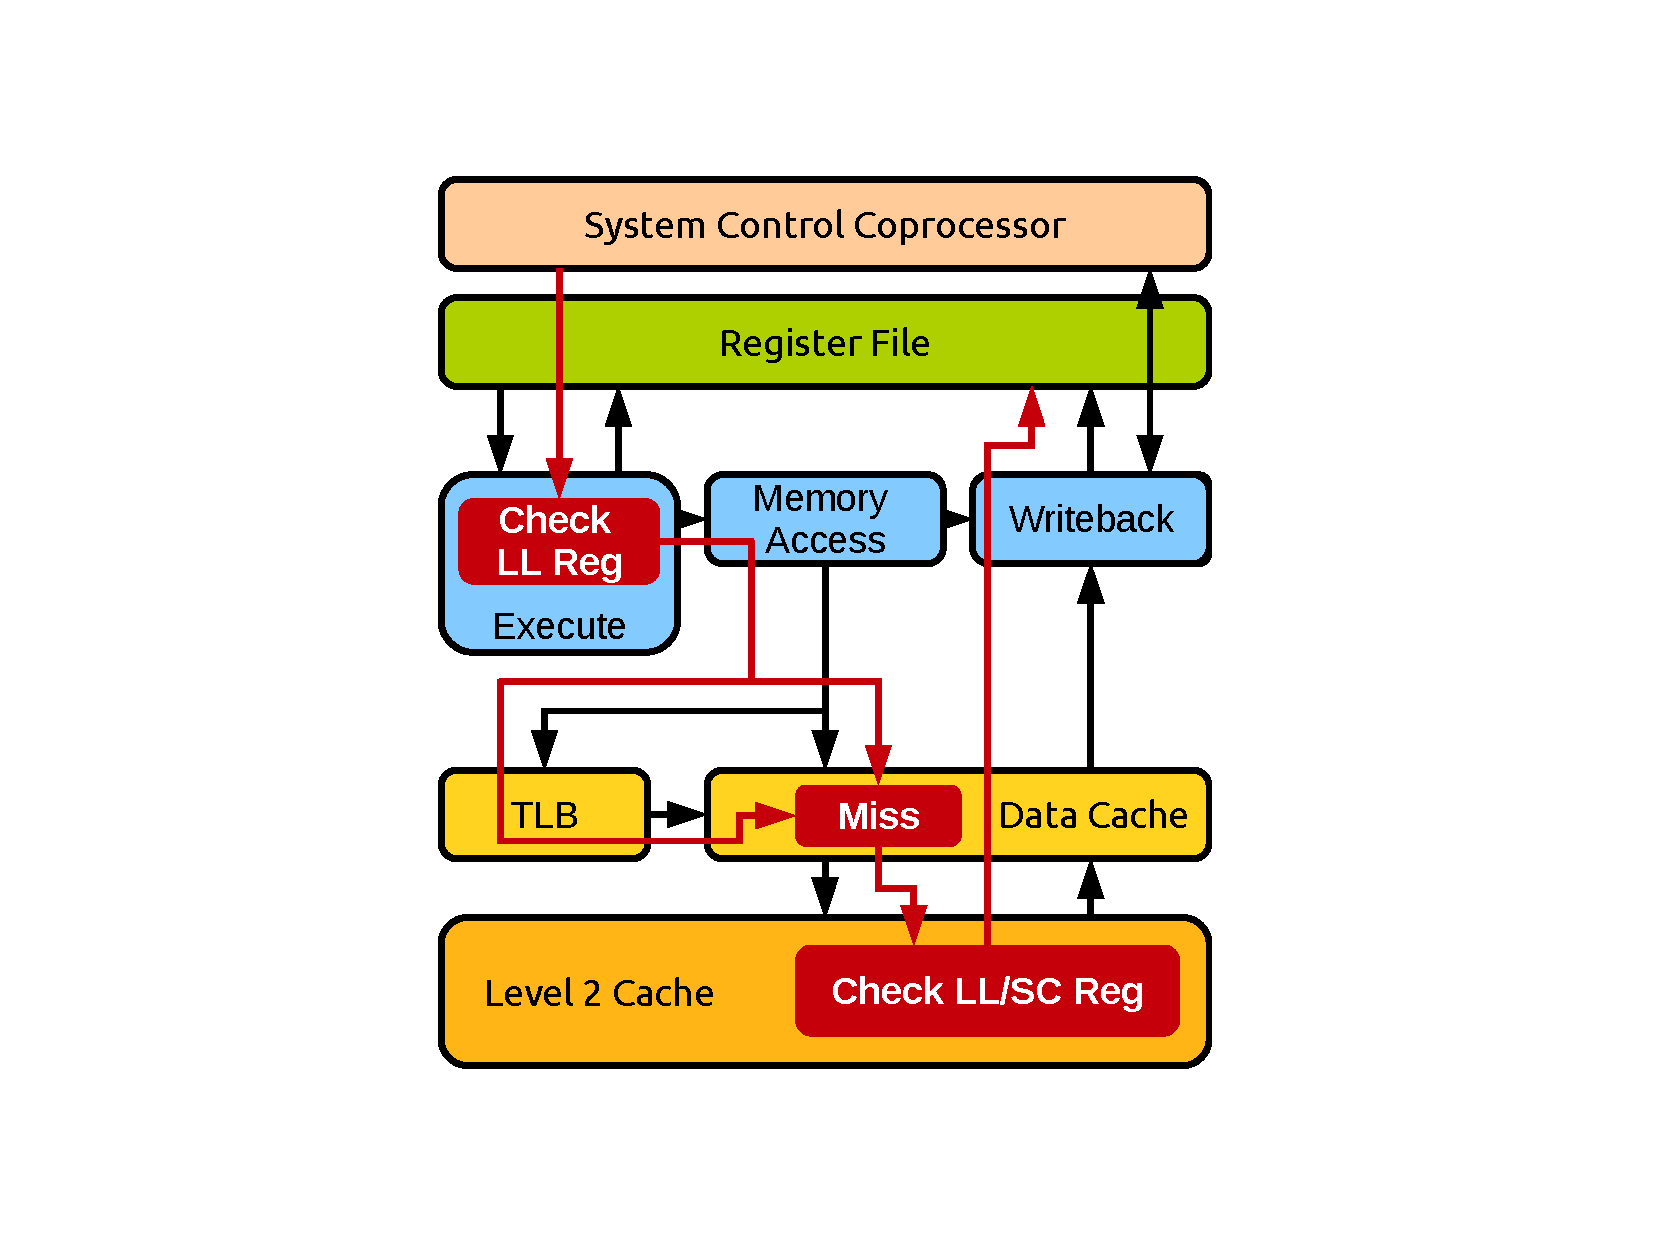
\includegraphics[trim={0 2.9cm 0 3cm},clip,width=\textwidth,height=\textheight,keepaspectratio]{BERI_llsc}}
				\caption{BERI LL/SC mechanism} 
				\label{beri_llsc}
		\end{figure}
		%\vspace{-5mm}

		Significant differences in the coherence schemes have necessitated a generalised LL/SC design. In order to avoid any memory consistency issues, all memory locations are propagated directly to the shared L2 cache. This ensures up-to-date data observations. This scheme adds latency overheads, however, a relatively low occurrence of LL and SC instructions and expected losses due to synchronisation, permit this implementation.
		
		The L2 cache holds one LL/SC register per core interface, the MIPS specification does not expect more than one LL operation at a time. An LL is treated as a miss in the private L1 data cache. If an SC hits in the private cache, the memory location is invalidated and the SC is written through into the L2. The pipeline expects a success or fail for each SC operation and unlike normal stores, the L2 returns a success flag to the L1.
		
		In addition to LL/SC, software often uses other synchronisation mechanisms such as the MIPS SYNC instruction. Unlike LL/SC, the behaviour of SYNC instructions is more dependent on the memory consistency model.

\section{FPGA Implementation}
	\label{fpga_implementation}
	The BERI processor and its variants can be synthesised for an FPGA. We use the Terasic DE4 board equipped with a Stratix-4 FPGA. The board includes dual DDR2 sockets, USB (debugging and testing via JTAG), PCI-E, Gigabit Ethernet, SD-Card support (used for file transfer), SATA, and other interfaces.
	
	\begin{figure}
	\setlength{\fboxsep}{0pt}%
	\setlength{\fboxrule}{1pt}%
	%\setlength{\fboxrule}{0pt}%
	
		\vspace{-6mm}
		\begin{subfigure}[b]{1\linewidth}
		\centering
		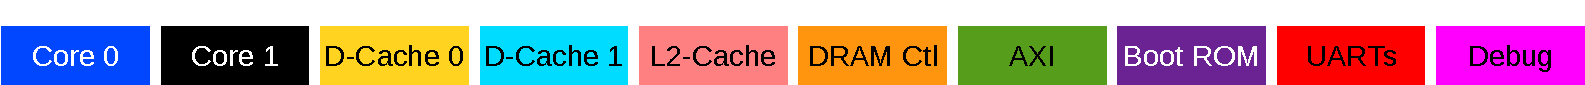
\includegraphics[width=0.92\linewidth]{quartus_dualcore_legend}
		%\caption{Core Pipelines} 
		%\label{dualcore_quartus:b} 
		%\vspace{4ex}
		\end{subfigure} 
		\vspace{-2mm}

\begin{comment}
		\begin{subfigure}[b]{1\linewidth}
		\centering
		\includegraphics[width=0.83\linewidth]{quartus_dualcore_full}
		\vspace{4ex}
		\end{subfigure}%% 
		\caption{Quartus Dual-Core FPGA Layout}
		\label{dualcore_quartus_full}
\end{comment}
		
%\begin{comment}
		\begin{subfigure}[b]{0.5\linewidth}
		\centering
		\fbox{\includegraphics[width=0.83\linewidth]{quartus_dualcore_full}}
		\caption{Complete design} 
		\label{dualcore_quartus:a} 
		\vspace{4ex}
		\end{subfigure}%% 
		\begin{subfigure}[b]{0.5\linewidth}
		\centering
		\fbox{\includegraphics[width=0.83\linewidth]{quartus_dualcore_cores}}
		\caption{Two processor pipelines} 
		\label{dualcore_quartus:b} 
		\vspace{4ex}
		\end{subfigure}
		\begin{subfigure}[b]{0.5\linewidth}
		\centering
		\fbox{\includegraphics[width=0.83\linewidth]{quartus_dualcore_memory}}
		\caption{Memory hierarchy} 
		\label{dualcore_quartus:c} 
		\end{subfigure}%%
		\begin{subfigure}[b]{0.5\linewidth}
		\centering
		\fbox{\includegraphics[width=0.83\linewidth]{quartus_dualcore_caches}}
		\caption{Cache hierarchy} 
		\label{dualcore_quartus:d} 
		\end{subfigure} 
		\caption{Dual-core BERI, Quartus FPGA layout}
		\label{dualcore_quartus}
%\end{comment}
	\end{figure}

\begin{comment}	
	\begin{figure}[!h]
		\centering 
			\makebox{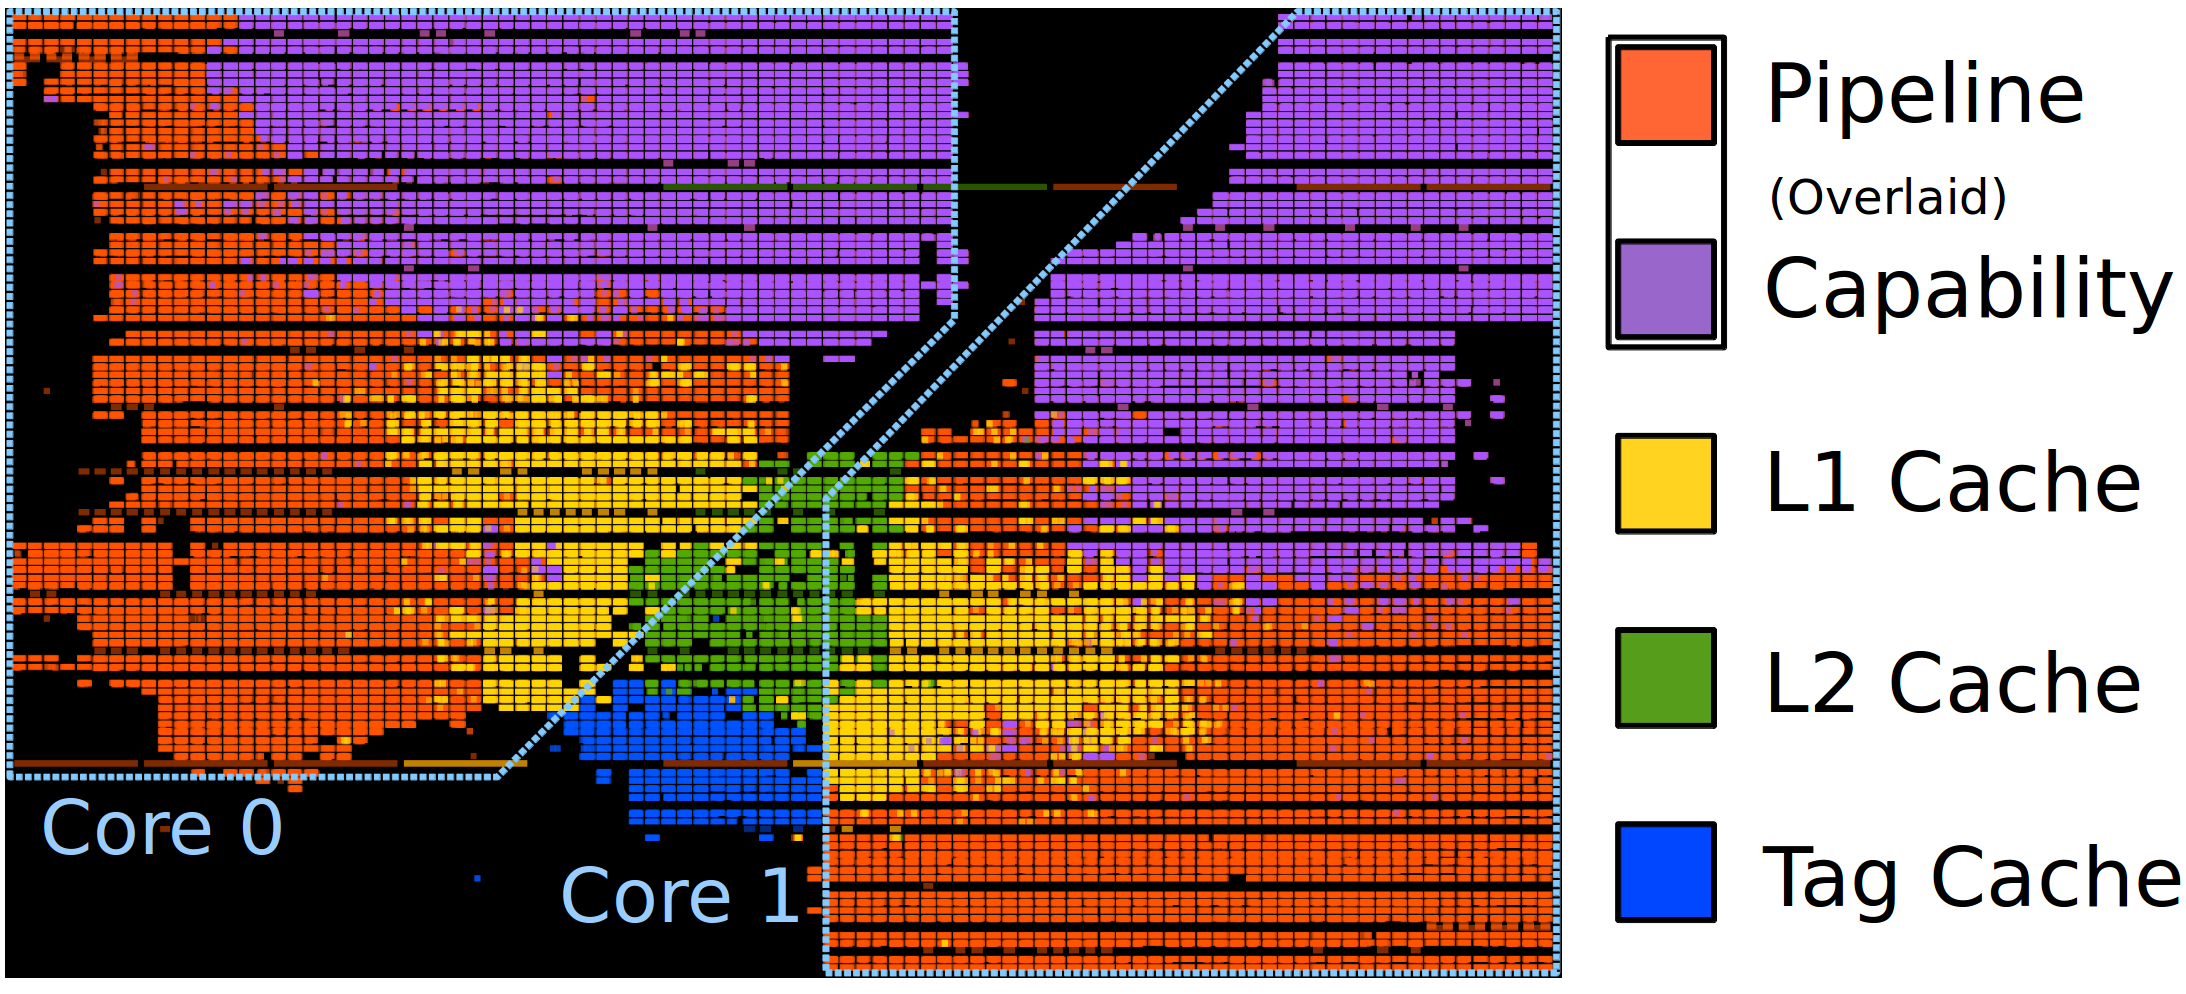
\includegraphics[width=\textwidth,height=\textheight,keepaspectratio]{dualcore_fpga}}
			\caption{Dual-Core BERI FPGA Layout} \label{dualcore_fpga}
	\end{figure}
\end{comment}

	The Bluespec compiler can produce verilog which is synthesizable through the Altera Quartus tools. Figure \ref{dualcore_quartus} shows the Quartus synthesised layout of the BERI dual-core processor. Due to the visualisation features of Quartus, some architectural components are overlaid and may not be correctly scaled. Specifics of the coherence mechanism are difficult to differentiate in the layout tool, and look almost identical. The images shown have been generated from a directory design.
	
	\begin{description}
		\item[(a)] Layout of dual-core BERI components: two BERI pipelines, two private data caches (D-Cache's), shared level 2 cache, DRAM controller, boot memory, AXI bus interface, two UARTs, and the debug units. It is not possible to highlight the PIC's as they mostly consist of wiring and minimal logic. The L1 data caches appear larger than normal, as they communicate with the TLB, pipeline stages, and other processor components. As a result the cache logic is spread over a large portion of the FPGA.
		\item[(b)] Two processor pipelines. The L1 instruction caches are included in the highlighted regions.
		\item[(c)] The memory, hierarchy and interconnect are visible in this image. The memory merge unit is not visible, located within the overlapping L1 and L2 logic regions.
		\item[(d)] Two L1 caches and the shared L2 are shown. 
	\end{description}
	
	All the multiprocessor versions of BERI used in this dissertation operate at 100MHz. The DRAM module operates at 200MHz and typically has a capacity of 1GB. BERI dual-core directory version utilizes approximately 58\% of the FPGA logic, with the time-based version requiring around 57\%.

%\clearpage
\section{Testing and Debugging}
	A range of test frameworks have been developed for the BERI project by a large number of people including Robert Watson, Simon Moore, Jonathan Woodruff, Michael Roe, Brooks Davis, David Chisnall, Alexandre Joannou, Theo Markettos, Robert Norton, Colin Rothwell, Stacey Son, Steven Murdoch, Nirav Dave, Matthew Naylor, and myself (Members of the CTSRD project \cite{ctsrd15}). Most of these tests have been used to validate the architectural properties of our system.

	\subsection{Hardware and Software Tracing}
		BSV provides display statements, equivalent to C language print. These statements are used for tracing and debugging when using Bluesim. The tracing technique is used by the Cheritest suite, AXE tests, and bare metal tests in simulation.
		
		Tracing and debugging in hardware is done through a dedicated debug unit, one per core. The debug unit injects instructions into the processor pipeline. These instructions are independent but may cause side-effects, as they are permitted to modify registers and memory. This module also maintains a trace buffer which can be used to log instructions in hardware.
	
	\subsection{Cheritest}
		This test suite is included in the BERI open-source project. There are over 2000 tests currently in the suite, ranging from basic arithmetic, to TLB operations and exception handling. The suite has been constructed by Robert Watson, Michael Roe, Stephen Murdoch, with test contributions from a number of CTSRD \& MRC2 project members \cite{CTSRD,MRC2}. I have added a range of tests for multi-core versions of the processor. This suite has been a critical part of the processor development.
		
		Processor models are regularly tested and verified through the Jenkins continuous integration framework. This automatic tool is currently generating Bluesim designs evaluated through Cheritest, as well as Quartus synthesised FPGA files.
		
	\subsection{Bare Metal Tests}
		In addition to Cheritest suite, we also use a set of bare metal, C language-based tests. Tests are compiled with GCC for MIPS 64-bit architectures. These tests allow us to check software compatibility without the need of an OS or hardware. They can also be loaded into an FPGA design. Some results obtained in Chapter \ref{chapter_validation} and \ref{chapter_sca} are based around the bare metal framework. 
		%Table \ref{vaucher_system_info} shows details of the testing environment. 
		Bare metal tests simulated through Bluesim are cycle accurate; underlying hardware characteristics should not affect the outcome. 

	\subsection{CHERI Litmus Tests}
		Litmus tests are discussed in detail in Chapter \ref{chapter_validation}. They are short tests, usually limited to a small number of instructions, designed to discern the memory consistency model of a given architecture. The CHERI Litmus tests \cite{CHERI_litmus} are designed to run bare metal on BERI/CHERI. These tests have been used to analyse the behaviour of the coherence schemes described in this dissertation.
		
	\subsection{Memory Consistency Checker}
		The AXE checker \cite{AXE_checker,bluecheck}, tests the memory subsystem in isolation and independent of the processor pipeline. Memory can be stressed much more as only memory instructions are repeatedly injected into the cache framework. Even the basic consistency models exhibit vast amounts of non-determinism. The checker tool exhaustively enumerates all behaviour of a set of memory operations. A general-purpose constraint-solver, Yices \cite{Yices15}, is used to check the traces for inconsistencies. These tests also permit a much faster execution and evaluation time. Every coherence model discussed in this dissertation has been verified through the AXE tool, further details are provided in following chapters.

		\begin{table}[b]
		\begin{center}
		\begin{tabular}{|l|l|}
			\hline		
			\multicolumn{2}{|c|}{Operating System} \\
			\hline
			FreeBSD & 11.0-CURRENT \#0 c2208dd(master) \\
			& Mon Dec 15 16:35:59 UTC 2014 \\
			\hline
			\hline		
			\multicolumn{2}{|c|}{Compiler Parameters} \\
			\hline	
			Compiler & clang version 3.6.0 \\
			Target & cheri-unknown-freebsd \\
			Thread model & posix \\
			\hline
		\end{tabular}
		\caption{FreeBSD environment}
		\label{freebsd_info}
		\end{center} 
		\end{table}
		
		\begin{comment}
		Copyright (c) 1992-2014 The FreeBSD Project.
		Copyright (c) 1979, 1980, 1983, 1986, 1988, 1989, 1991, 1992, 1993, 1994
			The Regents of the University of California. All rights reserved.
		FreeBSD is a registered trademark of The FreeBSD Foundation.
		FreeBSD 11.0-CURRENT #0 c2208dd(master): Mon Dec 15 16:35:59 UTC 2014
		\end{comment}

	\subsection{Benchmarks on FreeBSD}
		\label{freebsd_setup}
		FreeBSD is a open source, Unix-like operating system. A version of this OS is supported on BERI, and a capability enhanced version of the OS is supported on CHERI. Benchmarks and other tests based on FreeBSD, described in this dissertation, run on a single user multi-core version of the OS. The Splash-2 benchmark suite, side-channel attack tests, and other software is compiled for FreeBSD using the CHERI LLVM compiler \cite{Chisnall15,Chisnall14} (Table \ref{freebsd_info}).
		
	\section{Summary}
		The existing BERI uniprocessor and test suit have been extended to provide multi-core support, sufficient for a full OS bring up. This can be used on FPGA for performance or in simulation for detailed analysis. Later chapters exploit this framework to explore cache coherency and side-channel effects on complete systems running large-scale benchmarks and applications.
		
		
		
		
		
		
		
		
		
		
		
		
		
		\begin{comment}
				\begin{table}[!h]
				\begin{center}
				\begin{tabular}{|l|l|}
				\hline
				\multicolumn{2}{|c|}{Hardware Parameters} \\
				\hline
				Architecture          & Intel x86--64 \\
				CPUs                  & 32 \\
				%Threads per core      & 2 \\
				%Cores per socket      & 16 \\
				%Vendor ID            & Intel \\
				%CPU MHz               & 1200.000 \\
				%BogoMIPS             & 6585.73 \\
				%L1 cache's            & 32K \\
				%L2 cache              & 256K \\
				%L3 cache              & 25600K \\
				\hline
				\hline		
				\multicolumn{2}{|c|}{Software Parameters} \\
				\hline
				Compiler & mips-linux-gnu-gcc \\ 
				& Debian 4.4.5-8 \\
				Assembler & mips64-as \\
				Linker & mips-linux-gnu-ld \\
				\hline
				\end{tabular}
				\caption{Simulation Environment}
				\label{vaucher_system_info}
				\end{center} 
				\end{table}
				%\vspace{-10mm}
		\end{comment}

% 3 lines below ensure that there is a blank page before a new chapter
\clearpage
\thispagestyle{empty}
\mbox{}
%TODO: Coherence
\makeatletter
%\newcommand{\rmnum}[1]{\romannumeral #1 }
%\newcommand{\Rmnum}[1]{\expandafter\@slowromancap\romannumeral #1@}
\makeatother
\ifpdf
\graphicspath{{Chapter1/Chapter1Figs/PNG/}{Chapter1/Chapter1Figs/PDF/}{Chapter1/Chapter1Figs/}}
\else
\graphicspath{{Chapter1/Chapter1Figs/EPS/}{Chapter1/Chapter1Figs/}}
\fi

\chapter{BERI Coherence Models}
\label{chapter_coherence}

In this chapter I introduce the BERI cache coherence protocols. I discuss the architectural details of both designs, including all optimisations added through evaluations in simulation and FPGA hardware. The parallel performance of the coherence protocols is presented in Chapter \ref{coherence_eval}.

The BERI directory-based coherence scheme uses a full directory approach. It tracks private sharer caches through a shared last level cache. This coherence scheme complies with the TSO memory consistency model, typically used on x86 systems.

The BERI time-based coherence protocol, assigns a timestamp to every cached line. This allows the protocol to forego coherence messaging. It uses standard memory communication to fetch data whenever an expired cache line is accessed. This protocol requires the appropriate usage of software synchronisation and locking instructions. 
However, no dedicated software support is necessary as barriers and locks are widely used by software.

A well defined memory consistency model is critical to provide software assurances. The time-based coherence scheme supports RMO memory consistency, specifically RMO{\large$^\star$} (defined in Section \ref{background_consistency}). The compliance of this cache coherence scheme is thoroughly verified through memory consistency checking tools presented in Chapter \ref{chapter_validation}. 

A relaxed memory consistency model may offer some parallel performance advantages, however, the main reason for selecting this model is that it simplifies the hardware design constraints and eliminates the need for any explicit coherence messaging. Additionally, it is widely supported by popular operating systems such as FreeBSD, and compilers such as LLVM. This memory model is also used in commercial architectures such as ARM and PowerPC. In its current form, the time-based coherence protocol cannot support a stronger coherence model, but stronger support is typically unnecessary.


\clearpage
\section{BERI Time-Based Coherence}
	\label{section_timebased_coherence}
	Communication centric cache coherence protocols focus on a bottom up approach, maintaining and distributing coherence information through the last-level cache (LLC) or a dedicated memory controller.
	The time-based coherence model goes against this principle by controlling coherence from within the private caches.
	In the absence of explicit coherence messaging, cache flushing is one way of updating stale data and restoring system coherence. 
	Behavioural correctness of the time-based coherence model relies on implementation elements such as the cache self-invalidation technique, explicit synchronisation instructions, and lock-free atomic instructions. 

	Software data structures are often stored contiguously in memory, and repeated data operations can be significantly sped-up through caching. Thus, choosing an appropriate cache line lifespan in a time-based coherence cache is non trivial. There is a constant tradeoff between miss rates due to counter overflows and the cache capacity overheads. In order to retain the benefits of data caching, the lifespan of each line must be long enough to maintain a low miss rate, as well as short enough to allow timely stale data eviction. This coherence model does not directly expose cache line time-outs, so software must use correct locking structures and barriers to ensure appropriate data sharing.

	\subsection{Time Counter}
		In the current BERI multiprocessor implementation, each L1 data cache has a dedicated time-counter. This counter governs the cache self-invalidation policy. The time-counter increments are dictated by the cache cycle counter and the synchronisation (SYNC) instruction. 
		The maximum tick range of the cycle counter can be selected during hardware synthesis and currently is not modifiable through software.
		
		Every time-counter tick can be referred to as the time-out, since all cache lines loaded prior to the tick become invalid.
		Figure \ref{beri_timebased_algorithm} illustrates this behaviour.
		A full cache flush is triggered when the time-counter rolls over, this is done using the cache initialisation logic, all memory access to the cache are blocked during this flush. Frequent counter roll-overs may result in a slow cache response time, so there is a tradeoff between the counter size and cache storage overheads. 

	\subsection{Tag Timestamp}
		Each L1 data cache line contains data bits and tag bits, stored in separate memory blocks. A timestamp is added to the tag bits, this tag-time-stamp (TTS) dictates the cache line lifespan. TTS is set when a line is cached for the first time, this value is generated by adding 1 to the current time-counter.
		When a cache line is requested and it is a hit, the TTS is compared to the current time-counter value. Line lifespan expires when the time-counter is greater than TTS, this forces a cache miss. A valid TTS allows the cache to proceed as normal.

		\begin{figure}[t]
			\centering 
				\makebox{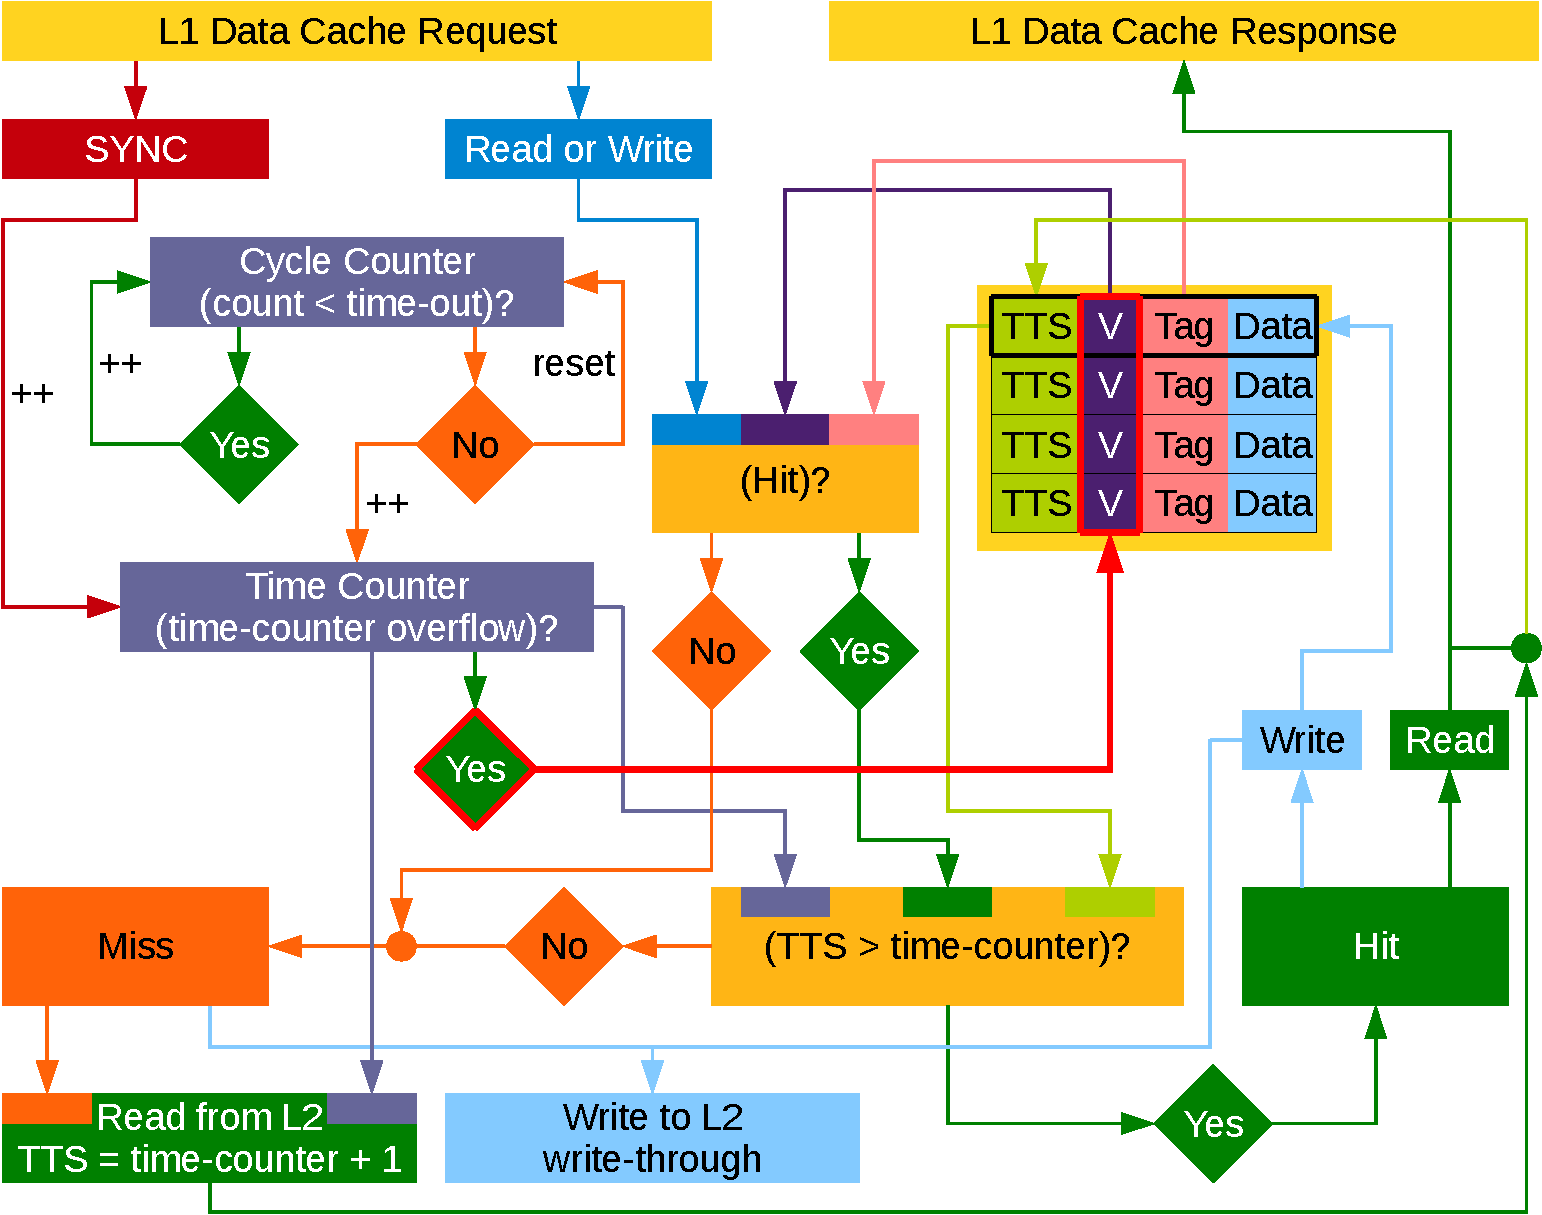
\includegraphics[width=\textwidth,height=\textheight,keepaspectratio]{BERI_timebased_algorithm}}
				\caption[BERI time-based coherence mechanism]{BERI time-based coherence mechanism (L1 data cache)} 
				\label{beri_timebased_algorithm}
		\end{figure}
	
	\subsection{Time-out Selection}
		Time tick granularity used for self-invalidation is dictated by the cycle counter. It can be varied from a single cycle to infinity. In the evaluation chapter we will see how the choice of cache line time-outs affects system performance. Its easy to assume that long time-outs will keep data cached and benefit overall performance, however, holding on to shared data and waiting for SYNCs does not fit all software behaviour. 		
		The performance of software relying on polling operations may suffer due to infrequent data updates. Polling operations rely on updates to memory locations and may not use any SYNC instructions, hence, time-outs are necessary. 
		
		Eliminating cache time-outs may result in unpredictable OS behaviour, an increased likelihood of deadlocks, and an overall performance drop. 
		The time-out procedure ensures some progress, regardless of other synchronisation operations. However, waiting for a time-out could cause lengthy delays. Some memory polling patterns can be detected by hardware.
		
		Software relying on lock-free atomic instructions is not affected by time-outs; on multi-core BERI these instructions bypass local caches. They are frequently used for synchronisation. Additionally, a generous use of SYNCs in FreeBSD allows time-based coherence to function correctly. FreeBSD synchronisation and locking statistics are detailed in Chapter \ref{coherence_eval}, coherence results and evaluation. Deadlock avoidance is discussed in Section \ref{litmus_perfromance}.

	\subsection{Polling Detection Mechanism}
		\label{polling_detection_mechanism}
		This L1 cache based mechanism eliminates one of the major drawbacks of time-based coherence; slow updates to polled memory locations, caused by stale data caching and a potentially large cycle delay between self-invalidates. OS schedulers may use memory polling as a part of the scheduling mechanism. The access patterns can be predicted in hardware, leading to a reduction in memory overheads. The OS polling behaviour and profiling techniques are illustrated by Frigui and Alfa \cite{Frigui95}.  Further motivations and design choices of the BERI polling optimisation are explained in Section \ref{sync_only_coherence}, SYNC-only coherence. 

		\begin{figure}[!t]
		\begin{tcolorbox}[
		colback=cyan!1!white,
		colframe=cyan!75!black]
\begin{center}
\begin{BVerbatim}
if (read hit)  // query polling table
	if (valid && address match)
		delete table entry;
		force read miss;
	else
		return data;
if (write hit) // query polling table
	if (valid && address match)
		delete table entry;
		write-through data;
	else
		write local data;
		write-through data;	
if (read miss) // fetch data from L2
	if (empty polling table entry)
		add new address;
	else
		delete random entry;
		add new address;
	return data;
if (write miss) // non write allocate
	write-through data;
\end{BVerbatim}
\end{center}		
		\end{tcolorbox}
		\caption{L1 data cache memory polling detector}
		\label{polling_detector_diagram}
		\end{figure}

		The detector tracks cache load misses. When the data is fetched, it saves the physical addresses into a 4 register fully associative lookup table. 
		The physical address of each new cache load request is compared against valid entries in the detector lookup table. 
		An address match indicates that the requested memory location has not been locally updated since it was first loaded. 
		This behaviour is typically exhibited by a memory polling operation. 
		When such a memory location is identified, a miss is forced by the detector and an updated value is fetched from shared memory. 
		The pseudocode for this algorithm is presented in Figure \ref{polling_detector_diagram}.
		
		Table entries are deleted whenever a store matches one of the entries. A random replacement policy is used whenever the table runs of empty memory slots. Based on FreeBSD observations, a 4 entry table should be sufficient. 
		However, some software behaviour may be different, and more table entries or an alternative detection technique may be necessary.
		In the event of a polling misprediction, the time-based automatic self-invalidation mechanism ensures that stale data will be eventually updated and some progress will be made.
		
		Time-based coherence benefits from this mechanism, as it significantly speeds up synchronisation through polling.
		The algorithm is independent of the coherence model and could be added to other schemes.
		However, designs such as the directory approach are unlikely to benefit from polling detection, since the coherence scheme itself ensures stale data eviction.
		Furthermore, false polling detection is likely to cause a performance degradation.
	

	\subsection{TTS Memory Overhead}
		\label{tts_memory_overhead}
		There is a tradeoff between the time-counter register size and the penalty for counter roll-overs. A smaller time-counter size increases the frequency of roll-overs, leading to frequent full cache flushes. Note that time-counter size is independent of the number of cycles per time-counter tick. 
		Darnell and Kennedy \cite{Darnell93} have shown that cache line timestamps as low as 1 bit can be used. However, their scheme relies on explicit software epochs aimed at select memory locations. The SYNC instruction has a similar effect in the BERI time-based scheme, but the cache can also automatically self-invalidate lines. 
		
		In more recent work by Elver and Nagarajan \cite{Elver14}, 4 bit timestamps are added to memory locations, reducing the sharer tracking overheads of MESI coherence (Chapter \ref{chapter_background}). I have opted to use a 4 bit TTS size, as the storage overheads for two L1 data caches (2$_{cores}$$\times$4$_{bits}$$\times$512$_{l1-lines}$ = 4096) is identical to the directory overhead in the L2 cache (2$_{cores}$$\times$1$_{bit/core}$$\times$2048$_{l2-lines}$ = 4096). Figures \ref{dcache_tags_short_tts} and \ref{big_dcache_tags_short_tts} compare tag overheads with increasing cache capacity (tags have been padded to 32 bits in order to simplify the visual comparison). 
		
		The counter size must be carefully considered when synthesising these caches on an FPGA, as block RAM (BRAM) design will greatly affect optimisation. The tag size tradeoff is also critical, when a certain size is exceeded, multiple BRAM's may be necessary. ASIC designs are more flexible, as arbitrarily sized tags, data lines, and other components can be produced.

		\begin{figure}[t]
		\centering
			\newcommand{\colorbitbox}[3]{%
			\rlap{\bitbox{#2}{\color{#1}\rule{\width}{\height}}}%
			\bitbox{#2}{#3}}
			\definecolor{lightcyan}{rgb}{0.6,1,1}
			\definecolor{lightgreen}{rgb}{0.7,1,0.7}
			\definecolor{lightred}{rgb}{1,0.7,0.7}
			\definecolor{lightgray}{gray}{0.8}
			\begin{bytefield}[bitheight=\widthof{~Valid~},bitwidth=\widthof{\large x~},
			boxformatting={\centering\small}]{32}
			\bitheader[endianness=big]{31,30,27,26,25,0} \\
			\bitbox{1}{\color{lightgray}\rule{\width}{\height}} &
			\colorbitbox{lightgreen}{4}{TTS} &
			\colorbitbox{lightcyan}{1}{\rotatebox{90}{Valid}} &
			\colorbitbox{lightred}{26}{Tag}
			\end{bytefield}
			\caption[L1 data cache tags, 16KB cache]{L1 data cache tags, 4 bit TTS (16KB cache size)} \label{dcache_tags_short_tts}
		\vspace{5mm}

			\centering	
			\begin{bytefield}[bitheight=\widthof{~Valid~},bitwidth=\widthof{\large x~},
			boxformatting={\centering\small}]{32}
			\bitheader[endianness=big]{31,30,29,26,25,24,0} \\
			\bitbox{2}{\color{lightgray}\rule{\width}{\height}} &
			\colorbitbox{lightgreen}{4}{TTS} &
			\colorbitbox{lightcyan}{1}{\rotatebox{90}{Valid}} &
			\colorbitbox{lightred}{25}{Tag}
			\end{bytefield}
			\caption[L1 data cache tags, 32KB cache]{L1 data cache tags, 4 bit TTS (32KB cache size)} \label{big_dcache_tags_short_tts}
		\end{figure}
		
		Our RISC processor only requires 40 bits of physical address space. When the cache size is increased, fewer tag bits are required since fewer address bits are stored in the tags. Figure \ref{big_dcache_tags_short_tts} shows this effect when the cache size is doubled. 
		One additional bit will be used for cache indexing, so the tag is shrunk. This can be beneficial for time-based coherence, since a larger TTS can be used without increasing the relative storage overheads.
		
		The time-based coherence model does not add any overheads to the L2 cache and the LL/SC mechanism is identical to the one used by BERI directory coherence. The L2 cache tag structure for the time-based coherence mechanism and the LL/SC overheads are discussed in Section \ref{dir_llc_structure}, and compared against the directory-based coherence model.
		
	\subsection{SYNC Instruction Behaviour}
		\label{sync_behaviour}
		This instruction performs two operations in the L1 data cache. 
		Firstly, the time-counter is incremented on SYNC (Figure \ref{beri_sync}), ensuring that all stale data will be treated as invalid, it can also be interpreted as a single instruction full cache flush. 
		Note that if the SYNC instruction causes the time-counter to overflow, then the cache is reinitialised. 
		
		The second property of this instruction is to ensure that all loads/stores have been propagated to the LLC. 
		This is achieved by performing a flush to LLC, this memory access has no side-effects. The operation blocks the cache until a response is received. The response guarantees load/store propagation from the given core. The response is ignored by the pipeline as SYNC instructions are not expected to respond. 
		The SYNC mechanism used in the directory coherence model is also shown in Figure \ref{beri_sync} for a direct comparison. Since the directory does not use time-counters, the SYNC instruction simply ensures that all memory operations have propagated to the shared cache.
		
		Instruction caches do not self-invalidate; coherence is not necessary for instructions as long as self-modifying code is not executed.
		
		\begin{figure}[t]
			\centering 
				\makebox{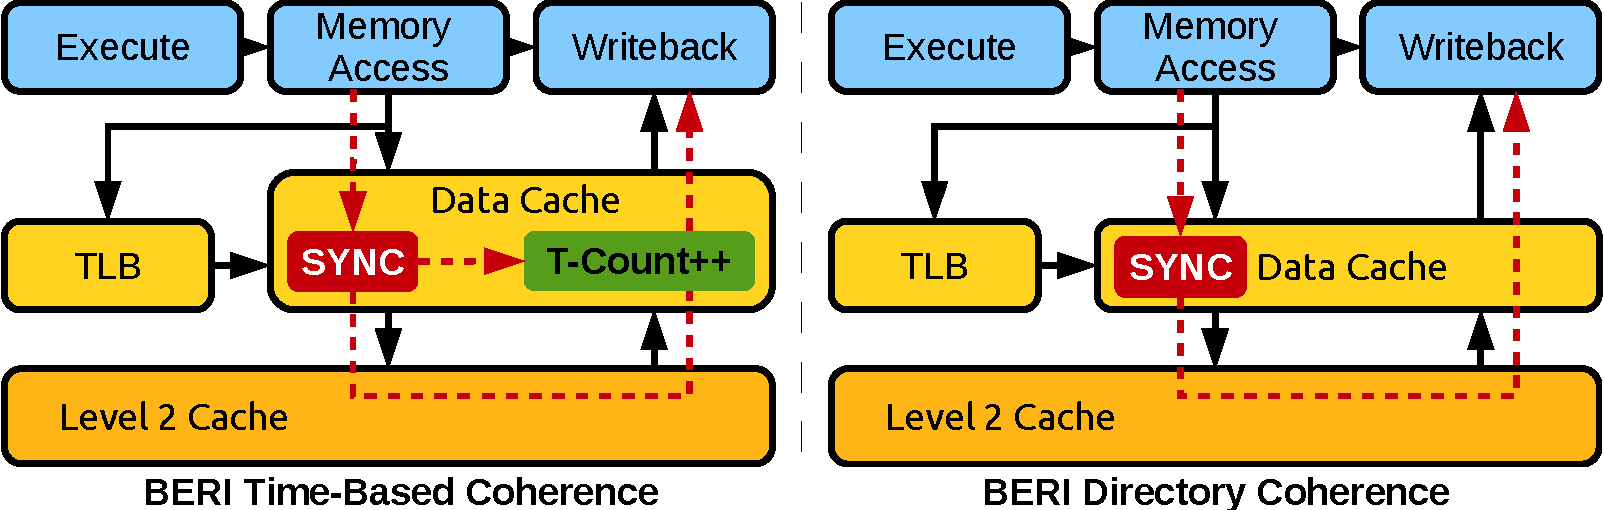
\includegraphics[width=\textwidth,height=\textheight,keepaspectratio]{BERI_sync}}
				\caption{BERI multiprocessor SYNC mechanism} 
				\label{beri_sync}
		\end{figure}


%\clearpage
\subsection{SYNC-only Coherence}
	\label{sync_only_coherence}
	
	%TODO: cost per invalidate for directory coherence
	
	%We have established that time-based coherence presents a functional memory consistency model, usable and supported by FreeBSD. In the evaluation Chapter \ref{coherence_eval} we will see that time-based coherence tends to show better parallel performance with increasing cache line lifespan. We have also seen the effects of a SYNC instruction on the cache behaviour. 
	
	It is possible to design a coherence scheme relying solely on SYNC instructions, using neither self-invalidation or coherence messaging. However, a few potential limitations include: insufficient or incorrect usage of synchronisation primitives, polling, and other schemes relying on strong hardware coherence.
	Memory polling operations can be implemented through other software primitives, without any need for special instructions. Alternatively, a hardware polling detection mechanism can be used, but it may not be able to detect and resolve all cases.
	
	For instance, on a dual-core BERI system, the FreeBSD booting mechanism uses core 0 by default. Once the initial boot set-up is complete, core 0 signals core 1 through shared memory and initiates parallel tasks. Core 1 waits for the update by running a simple loop consisting of a load instruction followed by a branch. It is easy for hardware to detect this operation as all core 1 memory accesses are loads to the same address with no local updates. The polling detector can be implemented by using a single register in each private cache to track a load to an unmodified location. One register is sufficient in this example but it may be insufficient in other scenarios.
	
	A hardware instruction trace of the FreeBSD file copy application (CP) has shown that during its execution a two stage polling operation is observed. The trace shows two loads to independent memory locations, separated by branch instructions. Software jumps between the two load operations with no other memory instruction in between. At least two polling detection registers are required to correctly identify this behaviour. 
	
	Testing on FreeBSD has not revealed polling mechanisms requiring more than two separate load addresses, such as the CP scenario. I implemented an in cache, 4 register polling detector, that complements the self-invalidation mechanism. 
	The polling detector is sufficiently wide to track most polling operations, and long delays between self-invalidations retain the hit ratios required by parallel applications. If this mechanism were to guarantee precise detection of all polling accesses, cache time-outs could be eliminated entirely and all coherence operations would be controlled through synchronisation instructions.


%\clearpage
\section{BERI Directory Coherence}
	\label{section_directory_coherence}
		The BERI multiprocessor architecture was initially designed using more conventional coherence mechanisms, unlike the time-based scheme discussed previously. The BERI directory-based design is the outcome of a refined exploration of communication centric coherence protocols.

		One of the simplest coherence protocols for a shared memory system is Invalidate On Write (IOW) \cite{Hennessy06}. Coherence is maintained by broadcasting invalidation messages whenever a store operation is performed in the shared cache. This protocol requires a cache write-through policy, since a write-back policy will allow the cache to hold dirty lines until they get evicted. Without explicit barriers or other means of data propagation, coherence will fail. The IOW coherence mechanism suffers large coherence communication overheads, since every store operation generates a broadcast message \cite{Lawrence98,Tomasevic92,Hennessy06}. 
		
		\textcolor{red}{Many have said that write-through data caches (private) are not actively used in modern CPU's, however, the recent generations of AMD processors have all relied on this cache data propagation protocol. (TODO: citation http://www.realworldtech.com/bulldozer/9/)}
		
		
		
		
		\textcolor{red}{Copy of the document starts here >>>>}
		 Since the L1D is both write-through and mostly included in the L2, evicting a cache line from the L1D is silent and requires no further actions. This is beneficial since evictions are typically caused by a filling a cache line, in response to a cache miss and closely tied to the critical path for a miss. In the exclusive L1D cache for Istanbul, moving the evicted line from L1D to L2 contributed to the latency for a cache miss.
		
		The relationship between the L1D and L2 caches also simplifies reliability. Since any data written by the L1D is also present in the L2, parity is sufficient protection for the L1; any errors can be fixed by reloading from the ECC protected L2 (or L3/memory). As a result, ECC is no longer required for the L1D (as it was for Istanbul), which reduces the power consumption for stores. In Istanbul, any store to a cache line had to first read to get the ECC, then recalculate the ECC with the new data and then finally write to the cache.
		
		While the L1D is mostly included in the L2, there are some situations where lines can reside in the L1D without being present in the L2. As a result, the L1D may need to be snooped when another core misses in the L3 cache. This is extremely undesirable, since there will be substantial snoop traffic in a Bulldozer system which will cost both power and performance if the L1D caches must always be snooped by remote cache misses. In Nehalem, the L3 cache is inclusive precisely to eliminate this sort of snoop traffic. It stands to reason that Bulldozer was designed to eliminate snoop traffic to the L1D caches and instead have the L2 cache for each module handle all the coherency snoops for that module. Unfortunately, AMD was unwilling to disclose the precise nature of their coherency protocol at Hot Chips, so we will have to wait to find out more details.
		
		One disadvantage of a write-through policy is that the L1D caches do not insulate the L2 cache from the store traffic in the cache hierarchy. Consequently, the L2 cache must have higher bandwidth to accommodate all the store traffic from two cores, and any associated snoop traffic and responses.
		
		To alleviate the write-through bandwidth requirements on the L2, each Bulldozer module includes a write coalescing cache (WCC), which is considered part of the L2. At present, AMD has not disclosed the size and associativity of the WCC, although it is probably quite small. Stores from both L1D caches go through the WCC, where they are buffered and coalesced. The purpose of the WCC is to reduce the number of writes to the L2 cache, by taking advantage of both spatial and temporal locality between stores. For example, a memcpy() routine might clear a cache line with four 128-bit stores, the WCC would coalesce these stores together and only write out once to the L2 cache.
		
		Most implementations of Bulldozer (certainly Interlagos) will share a single L3 cache, which acts as a mostly exclusive victim buffer for the L2 caches in each module. Again, AMD would not disclose any information as it concerns the overall product, rather than the core itself. However, it is possible to make an intelligent estimate based on public information. Assuming that each Interlagos die will have 8MB of L2 cache for 4 modules, the L3 is most likely to be 8MB.
		
		AMD cannot afford to produce a die with 16MB of L3 cache on 32nm and 4MB is probably too small. When Barcelona was first released on 65nm, the L3 cache was 2MB – equal to the aggregate size of the four L2 caches. It seems reasonable that AMD would return to this arrangement. The associativity is an open question, but should be at least 16-way and more likely 32 or 64 way. It is also expected that AMD has further refined and improved the sharing and contention management policies in the L3 cache.
		
		Prefetching is another area where historically Intel has relentlessly focused, and AMD has lagged behind. Prefetching can be highly effective at reducing memory latency, and can lead to tremendous increases in performance – especially for workloads with complex data structures that tend to incur many cache misses. In Bulldozer, there was a tremendous amount of effort put into the prefetching that should yield good results. The exact nature of the strided prefetchers (i.e. where addresses are offset by exactly +/-N bytes) was not discussed, but that is an area which has been very thoroughly explored in academia and commercial products.
		
		More intriguing is Bulldozer’s non-strided data prefetcher, which is useful for accessing more complex and irregular data structures (e.g. linked lists, B-trees, etc.). Again, AMD did not disclose their approach, but one possibility is what we might describe as a ‘pattern history based prefetcher’. The prefetcher tracks the addresses of misses and tries to identify specific patterns of misses that occur together (temporally). Once a pattern of misses has been detected, the prefetcher will find the first miss in the pattern. When this first miss occurs again, the prefetcher will immediately prefetch the rest of the pattern. For traversing a complex data structure like a linked list, this would be a fairly effective approach. There are other techniques that have been discussed in academic literature, and it will be interesting to see which AMD implemented.
		\textcolor{red}{Ends here <<<<}
		
		\textcolor{green}{Also see: http://www.programcreek.com/2012/12/amd-versus-intel-successes-and-pitfalls-of-their-processor-architectures-2-bulldozer-and-sandy-bridge-comparison/}
		
		\textcolor{blue}{http://delivery.acm.org/10.1145/2620000/2618129/a4-molka.pdf?ip=128.232.64.58\&id=2618129\&acc=ACTIVE\%20SERVICE\&key=BF07A2EE685417C5\%2E6CDC43D2A5950A53\%2E4D4702B0C3E38B35\%2E4D4702B0C3E38B35\&CFID=832885662\&CFTOKEN=17969456\&\_\_acm\_\_=1472754966\_7ba3a70cc008174a88a56e87443dafc2}
		%http://delivery.acm.org/10.1145/2620000/2618129/a4-molka.pdf?ip=128.232.64.58&id=2618129&acc=ACTIVE%20SERVICE&key=BF07A2EE685417C5%2E6CDC43D2A5950A53%2E4D4702B0C3E38B35%2E4D4702B0C3E38B35&CFID=832885662&CFTOKEN=17969456&__acm__=1472754966_7ba3a70cc008174a88a56e87443dafc2
		
		
		
		
		\subsection{Tracking Shared Memory}
			The IOW design was significantly improved by using a directory to accurately track all sharers of a given memory location. The directory-based protocol closely resembles the full-map directory schemes described by Hennessy and Patterson \cite{Hennessy06}, Lilja \cite{Lilja93}, and Chaiken et al. \cite{Chaiken90}. 
			
			The directory is located in the shared last level cache (LLC) and sharers are tracked by maintaining one bit per core per cache line. A combination of all shared bits for a given line is a sharers list. The list indicates whether that line is also present in one of the private caches. When the shared line receives a store operation, the sharers list identifies caches holding stale data copies. The LLC sends a coherence message to a memory controller. 
		
			The memory controller simply reads the sharers list contained within the message and then distributes invalidates to all relevant private caches. The coherence network and the memory controller are isolated from other memory communication. This allows low latency invalidate distribution. Additionally, the invalidate messages take priority over other requests in private caches. 
			
			% I-Caches
			I choose not to enforce coherence in the instruction caches, which is normally required for self-modifying code, commonly used by loaders/dynamic linkers which are capable of handling explicit software-directed instruction cache invalidation.

		\subsection{Inclusion Policy}
			Protocol correctness necessitates an accurate list of sharers, enforced through a strict cache inclusion policy. This policy indirectly affects the directory performance, since sharers must be carefully tracked and invalidated when a capacity miss is encountered. This issue is elaborated by Gupta et al. \cite{Gupta90}. 
			
			Similar to other coherence protocols requiring explicit coherence messages, the BERI directory protocol shows some communication drawbacks, not very evident with a small number of cores, but likely to escalate as the number of cores is increased in the future. 
	

		\subsection{Coherence Messaging Overheads}
			% Doesnt need ACK
			The protocol does not require coherence message acknowledgements, unlike some schemes described by Martin et al. \cite{Martin12}. This is achieved through fine tuning of coherence message delivery ensuring strong consistency compliance (TSO). Strong consistency has ensured stable FreeBSD OS support and allowed the development of the BERI multiprocessor system.
			
			Communication overheads are inevitable with a directory-based, snooping-based, or other novel communication based protocols \cite{Ros12,Hennessy06}.
			Research described in \cite{Lilja93,Sanchez12,Cuesta11,Cuesta13,James90} has shown a number of ways of optimising directory-based coherence designs through coherence message reduction, logic overheads, and understanding of sharing patterns.
			
			Relatively small scale testing of BERI has not yet necessitated these optimisations and the current protocol has been proven to work well, showing good private cache hit rates (see Chapter \ref{coherence_eval}). These characteristics provide sufficient evidence that the protocol is representative of directory-based coherence schemes and appropriate for a baseline comparison. 
		
		\subsection{Design Comparison}
			The BERI directory-coherence scheme is representative of an exact full directory mechanism. It is difficult to directly compare the BERI directory-based coherence design with other related designs, as most of the designs cannot be prototyped on the MIPS architecture without significant modifications or speculative execution. 
			
			Chapter \ref{coherence_eval} shows the performance evaluation of this protocol, the cache hit/miss ratios are comparable to non-optimised directory protocols, precision and efficiency of coherence messages is also shown. 
	
			BERI design complexity and Stratix-4 FPGA capacity currently limit the number of cores to 4. However, future design iterations and multi-FPGA interconnect could allow tens or hundreds of physical cores, necessitating a scalable coherence protocol. 
	
	\subsection{Data Cache Structure}
		\label{dir_data_cache_structure}
		The L1 data caches do not make any coherence decisions, unlike the BERI time-based model. Coherence data is supplied to the cache through a dedicated interface. The coherence message is processed by a dedicated hardware module within the cache, performing any necessary tag lookups and appropriate invalidates. Figure \ref{dir_dcache_tags} shows the tag structure for a BERI directory-based L1 data cache (tags have been padded to 32 bits in order to simplify the visual comparison). 
		
		In order to limit the side-effects of coherence messages on the general cache behaviour, an additional short-tag bank has been added. It is an optimisation and the directory scheme can be implemented without this feature. Figure \ref{dir_dcache_short_tags} shows the tag structure for an optimised directory coherence L1 data cache. The short-tag optimisation allows parallel memory access and coherence tag lookups. The short-tags are a subset of the complete physical address tag. 
		
		\begin{figure}[t]
		\centering
			\newcommand{\colorbitbox}[3]{%
			\rlap{\bitbox{#2}{\color{#1}\rule{\width}{\height}}}%
			\bitbox{#2}{#3}}
			\definecolor{lightcyan}{rgb}{0.6,1,1}
			\definecolor{lightred}{rgb}{1,0.7,0.7}
			\definecolor{lightgray}{gray}{0.8}

			\definecolor{lightorange}{rgb}{1,0.8,0.5}
			\definecolor{lightpurple}{rgb}{0.8,0.6,1}
			\definecolor{lightgreen}{rgb}{0.7,1,0.7}
			
			\definecolor{lightlightred}{rgb}{1,0.9,0.9}

			\begin{bytefield}[bitheight=\widthof{~Valid~},bitwidth=\widthof{\large x~},
			boxformatting={\centering\small}]{32}
			\bitheader[endianness=big]{31,27,26,25,0} \\
			\bitbox{5}{\color{lightgray}\rule{\width}{\height}} &
			\colorbitbox{lightcyan}{1}{\rotatebox{90}{Valid}} &
			\colorbitbox{lightred}{26}{Tag}
			\end{bytefield}
			\caption[L1 data cache tags, default]{L1 data cache tags, dual-core directory coherence (16KB cache size)} \label{dir_dcache_tags}
		\vspace{5mm}
		\centering
			\begin{bytefield}[bitheight=\widthof{~Valid~},bitwidth=\widthof{\large x~},
			boxformatting={\centering\small}]{32}
			\bitheader[endianness=big]{31,16,15,14,0} \\
			\bitbox{16}{\color{lightgray}\rule{\width}{\height}} &
			\colorbitbox{lightcyan}{1}{\rotatebox{90}{Valid}} &
			\colorbitbox{lightlightred}{15}{Short-Tag} \\
			\bitheader[endianness=big]{31,27,26,25,0} \\
			\bitbox{5}{\color{lightgray}\rule{\width}{\height}} &
			\colorbitbox{lightcyan}{1}{\rotatebox{90}{Valid}} &
			\colorbitbox{lightred}{26}{Tag}
			\end{bytefield}
			\caption[L1 data cache tags, short-tags optimisation]{L1 data cache tags, dual-core directory coherence with short-tags (16KB cache size)} \label{dir_dcache_short_tags}
		\end{figure}
		
		FPGA Block RAM's require 2 cycles to respond, one cycle to submit a BRAM request and one cycle to respond. During this operation all I/O ports of the cache are blocked. A subset of the tags is sufficient to reduce the number of false invalidates. Since parallel lookups are allowed, an invalidate operation only blocks the cache for 1 cycle instead of 2. This optimisation also helps maintaining a low coherence latency and simplifies TSO compliance. The drawbacks for using short-tags are the memory and logic overheads, however, FPGA synthesis results have not shown a significant impact in the L1 data cache size.

		An alternative to using short-tags would be either a full tag lookup or blindly invalidating cache lines. The former adds a cycle of latency and increases congestion where as the latter increases cache miss rates. As mentioned earlier, the short-tags are independently accessible and implemented in a separate BRAM. The size of the short-tags is such that for a given data cache capacity, all bits fit into a single BRAM. For this reason a total of 16 bits are used in a 16KB data cache, one valid bit and the 15 bottom bits of the physical address tag. 
		If the short-tags are valid and the select bits of the physical address match, the line will be invalidated. No action is taken otherwise. 
		
		Splash-2 Benchmarks (Chapter \ref{coherence_eval}) running on FreeBSD have shown that on an average, the short-tags optimisation offers a $\sim$2\% improvement in execution time over the full-tag version. All coherence messages issued by the directory result in some sharer cache blocking; short-tags simply reduce this penalty. This mechanism has been further analysed through memory consistency verification, bare metal tests, and correct FreeBSD behaviour. All directory-based coherence evaluation described in the dissertation uses this implementation.

		\begin{figure}[t]
		\centering
			\newcommand{\colorbitbox}[3]{%
			\rlap{\bitbox{#2}{\color{#1}\rule{\width}{\height}}}%
			\bitbox{#2}{#3}}
			\definecolor{lightcyan}{rgb}{0.6,1,1}
			\definecolor{lightred}{rgb}{1,0.7,0.7}
			\definecolor{lightgray}{gray}{0.8}

			\definecolor{lightorange}{rgb}{1,0.8,0.5}
			\definecolor{lightpurple}{rgb}{0.8,0.6,1}
			\definecolor{lightgreen}{rgb}{0.7,1,0.7}

			\begin{bytefield}[bitheight=\widthof{~Linked~},bitwidth=\widthof{\large x~},
			boxformatting={\centering\small}]{32}
			\bitheader[endianness=big]{31,28,27,26,25,24,23,0} \\
			\bitbox{4}{\color{lightgray}\rule{\width}{\height}} &
			\colorbitbox{lightpurple}{2}{\rotatebox{90}{Sharers}} &
			\colorbitbox{lightorange}{1}{\rotatebox{90}{Dirty}} &
			\colorbitbox{lightcyan}{1}{\rotatebox{90}{Valid}} &
			\colorbitbox{lightred}{24}{Tag}
			\end{bytefield}
			\caption[L2 cache tags, dual-core directory]{L2 cache tags, dual-core directory coherence (64KB cache size)} \label{dir_l2cache_tags}
		\vspace{5mm}
		\centering
			\begin{bytefield}[bitheight=\widthof{~Linked~},bitwidth=\widthof{\large x~},
			boxformatting={\centering\small}]{32}
			\bitheader[endianness=big]{31,30,29,26,25,24,23,0} \\
			\bitbox{2}{\color{lightgray}\rule{\width}{\height}} &
			\colorbitbox{lightpurple}{4}{\rotatebox{90}{Sharers}} &
			\colorbitbox{lightorange}{1}{\rotatebox{90}{Dirty}} &
			\colorbitbox{lightcyan}{1}{\rotatebox{90}{Valid}} &
			\colorbitbox{lightred}{24}{Tag}
			\end{bytefield}
			\caption[L2 cache tags, quad-core directory]{L2 cache tags, quad-core directory coherence (64KB cache size)} \label{dir_l2cache_tags_quad}
		\vspace{5mm}
		\centering
			\begin{bytefield}[bitheight=\widthof{~Linked~},bitwidth=\widthof{\large x~},
			boxformatting={\centering\small}]{32}
			\bitheader[endianness=big]{31,26,25,24,23,0} \\
			\bitbox{6}{\color{lightgray}\rule{\width}{\height}} &
			%\colorbitbox{lightpurple}{2}{\rotatebox{90}{Linked}} &
			\colorbitbox{lightorange}{1}{\rotatebox{90}{Dirty}} &
			\colorbitbox{lightcyan}{1}{\rotatebox{90}{Valid}} &
			\colorbitbox{lightred}{24}{Tag}
			\end{bytefield}
			\caption[L2 cache tags, dual-core time-based]{L2 cache tags, dual-core time-based coherence (64KB cache size)} \label{selfinv_l2_tags}
		\end{figure}

	\subsection{Last Level Cache Structure}
		\label{dir_llc_structure}
		The directory is fully contained in the LLC. Memory overheads are dramatically different between the time-based design and the directory design. The former incurs L1 data cache storage overheads, where as the latter incurs LLC storage overheads. The LLC must maintain a sharers list as specified previously. 
		
		The L2 cache overheads for the directory-based scheme are shown in Figures \ref{dir_l2cache_tags} and \ref{dir_l2cache_tags_quad} (tags have been padded to 32 bits in order to simplify the visual comparison). For comparison, the L2 cache tags for the time-based coherence model are also shown in Figure \ref{selfinv_l2_tags}. Since one bit per core is required to maintain directory coherence, the overhead is clear in Figure \ref{dir_l2cache_tags_quad}, where the costs double for a quad-core BERI. This is a typical scalability issue for a single level directory design.
		
		The shared LLC cache is write-back and maintains a fully inclusive cache policy. In order to maintain an accurate and updated sharers list, the LLC must hold copies of all the data present in the private data caches. 
		If a line is evicted from the shared cache, an invalidate must be broadcast to all sharer caches. Otherwise stale data may remain in L1 caches until the cache lines are replaced or re-fetched.
		
		The LLC cache stores tags on every memory operation. This is done to ensure that all cores accessing shared memory are included in the sharers list. 
		Failing to do so would result in inconsistencies and stale L1 data. If the OS issues a specific LLC cache invalidate instruction for a line that may be shared, all sharers of said line must be invalidated to preserve inclusion.

\clearpage
\section{Comparative Cache Design}
	\label{section_cache_properties}
	In this section I discuss how various cache design choices affect the memory coherence properties of multi-core BERI designs. The time-based model displays fewer design dependencies than the directory model, particularly when dealing with shared caches. However, it suffers a few drawbacks which are discussed below.

	\paragraph{Inclusion Policy:} This property is an attribute of a multi-tired memory hierarchy. The choice of an inclusion policy is design dependent. Maximising the total caching capacity necessitates an exclusive policy. A strictly inclusive policy requires all L1 data to be cached in lower levels as well. A non-inclusive policy permits intermediate behaviour between strictly inclusive and exclusive policies. 
	
	Shared memory communication centric coherence protocols benefit from a strictly inclusive policy, as shared memory is always aware of any privately cached data. The BERI directory model requires a strictly inclusive policy. 
	The time-based model does not require any explicit coherence messaging and any policy is acceptable. Since exclusive behaviour is not enforced, caches follow the non-inclusive policy.
	
	\paragraph{Associativity:} The storage location of a memory entry is determined by the replacement policy, ranging from direct mapped to fully associative. Maintaining coherence is simpler in direct mapped caches as all memory addresses will have a fixed location. Set associative or fully associative designs require parallel cache lookups in order to find any matching data. 
	
	Directory coherence is not directly affected by private cache associativity, however, multiple parallel coherence lookups may be necessary. Time-based coherence is not affected by associativity since coherence is only enforced during data loads or stores.
	
	\paragraph{Line Eviction:} When a cache runs out of free/invalid memory locations, the replacement policy dictates the cache line that will be replaced with new data. Direct mapped caches have a fixed policy; set associative caches can be designed with a number of cache replacement policies. The shared memory cache replacement policy will affect directory-based coherence, potentially increasing coherence messaging. Time-based coherence should not be affected, as no coherence messaging is used.
	
	\paragraph{Virtual and Physical Addressing:} Caches can be designed with various addressing modes, virtually tagged caches do not require TLB lookups where as physically tagged caches do. Coherence mechanisms benefit when shared caches and private caches use a common addressing mechanism, coherence messages are much simpler and cause fewer side-effects. All BERI caches are physically addressed, directory coherence messages carry the physical address and time-based coherence does not require messages.
	
	\paragraph{Cache Line Granularity:} BERI caches store 32 bytes of data per line. Each line shares a common valid bit and a tag field. An access miss to any word within a cache line will result in a full replacement. With the exception of aliasing which is discussed further, large lines are beneficial to both directory and time-based coherence. The memory metadata overheads are lower with a larger line size and coherence messages are more efficient as well. The tag-time-stamp used in time-based coherence has a smaller overhead as compared to a cache with a smaller line size. 
	
	\paragraph{Line Aliasing:} Mapping more than one data location to the same cache line results in aliasing. Aliasing is particularly hazardous in virtually mapped caches since two virtual addresses may point to the same physical address. Physically mapped caches are accesses through unique physical addresses, and aliasing usually results in the eviction of current cached data. Contention for the same cache line results in a degradation of performance and potential side-effects due to coherence.
	
	In coherent systems, such as the directory, memory aliasing can present a performance disadvantage. The directory must maintain an up-to-date record of any private caches sharing memory locations, when a memory line is evicted, the record must be updated as well. However, any sharers of the evicted line must be notified that the line is no longer in shared memory, failure to notify sharers will result in caching of stale data without any directory record. 
	%A strictly inclusive cache hierarchy will further exacerbate.
	
	Capacity misses in the shared cache will also result in evictions and coherence messages. This case has been observed in our directory based BERI design. The time-based coherence design is not penalised by the side-effects of aliasing memory since there is no explicit coherence messaging. Additionally this coherence model allows non-inclusive behaviour due to the absence of any sharer records. While time-based coherence has many drawbacks due to synchronisation and counter overflows, it does not suffer from aliasing overheads.
	
	\paragraph{False Sharing:} A subset of memory aliasing is false sharing of memory lines. It occurs when two memory words within a cache line are accessed independently and there is no direct data sharing. However, the coherence mechanism must keep track of any updates, particularly when the two words are accessed by different private caches. False sharing mostly results in performance degradation in the case of a directory design. As with aliasing, the time-based model is not affected by false sharing.
	
	\paragraph{Memory Operation Reordering:} Memory access reordering must behave according to a selected consistency scheme. TSO requires strict store ordering, whereas RMO permits interleaving of memory accesses. The TSO based directory coherence model must obey store ordering, necessitating precise and timely coherence messaging. The time-based coherence model uses RMO, requiring less intervention. Our cache design is fairly simple and does not offer memory access reordering within a core and its private caches, however, shared memory accesses may be out of order.
	
	\paragraph{Prefetching:} Compulsory cache misses can be reduces by fetching an entire line, when a memory word is requested. Advanced prefetchers can predict consecutive memory operations and speculatively fetch more than one line. Prefetching is beneficial for both the directory and time-based models. For both the directory and time-based design, the respective sharers list and tag-time-stamp are modified once, when the line is loaded into the cache.
	
	\paragraph{Alignment:} Any memory access that requires data between word boundaries is known as an unaligned access. Most modern systems permit unaligned accesses, the MIPS model used in BERI has a very limited support using special instructions. Since BERI does not permit accesses across cache line boundaries, we do not deal with this issue, however, as a general argument; aliment presents a challenge for both directory and time-based coherence. 
	
	The directory may require multiple sharer list accesses and the time-based model will require updating more than one TTS. Additionally a mismatched TTS may exist where one of the two lines was evicted and then reloaded. Accurate tracking of TTS entries will be necessary to avoid coherence bugs.
	
	\paragraph{Cache Instructions:} Most processors support some form of cache instructions, designed to allow cache cleaning, usually by the OS. In MIPS R4000, the cache instructions can target the L1 or the L2 caches. However, the effects of these instructions on coherence are not specified. In order to maintain the strict inclusion policy, the directory sends coherence messages to the L1 caches whenever a cache instruction evicts a shared line (applies to a single sharer scenario). Time-based coherence does not require strict inclusion, so L2 cache instructions have no effect. Respective consistency policies of the coherence schemes must also hold for cache instructions, this behaviour has been tested for both coherence models.
	
	\paragraph{Write Buffers:} Caches act as large write buffers, but many modern systems use an additional layer of buffering for improved memory accesses. Memory consistency mostly dictates the behaviour of write buffers. A TSO model requires correct write propagation through the write buffers. An RMO model allows a more relaxed behaviour, but the write buffers must propagate on synchronisation. BERI caches do not use write buffers, some buffering is present in the shared bus, but it does not affect the consistency models.
	
	\paragraph{Write Hit Policy:} There are largely two write hit policies: write-through and write-back. A write-through policy updates the current cache and propagates the update to a lower level of memory. Typically, write-back caches mark the line as dirty and hold the copy until the line is evicted or explicitly requested through coherence. BERI L1 caches are write-through. Both coherence schemes benefit from this behaviour. The write-back policy is frequently used in L1 caches, reducing memory traffic to the L2. Directory coherence requires more states to accurately track sharing patterns since writes are not immediately visible. Coherence schemes such as MESI, MOESI, MESIF, etc provide the necessary states for tracking sharing. 
	
	With write-through L1 caches, the time-based model is always guaranteed to fetch an up-to-date memory copy when a line is self-invalidated, since all stores are propagated to the L2. This approach is frequently used in related research \cite{Chen92,Choi11,Singh13,Singh14,Sung15}. 
	
	A write-back L1 will prevent the propagation of updates, but the time-based scheme can be adapted to deal with this scenario by tracking dirty lines, however, additional cache logic will be necessary. Overheads can be reduced by tracking a small number of dirty lines and periodically flushing them to the L2. This technique would allow batching of writes and reducing communication traffic, while retaining the advantages of time-based coherence. Dirty lines will need to be flushed on SYNCs, adding a performance penalty due to cache blocking during eviction. Periodic flushes and limiting the number of dirty lines may reduce this penalty.
	
	\paragraph{Write Miss Policy:} On a write miss, the cache can either request the line from a lower tier of memory and update it with new data (write allocate), or simply pass the write to a lower level of memory and leave the current cache untouched (non write allocate). BERI caches use the non write allocate policy. Directory and time-based coherence can accommodate both policies natively. A write allocate policy would perform a load from shared memory and a directory would register the requester as a sharer. The time-based model would assign a tag-time-stamp to the loaded and updated line.

\clearpage
\section{Coherence Hardware Overhead Comparison}
	\label{section_fpga_overheads}
	Coherence mechanisms typically add logic, wiring, and memory overheads. The overheads for the BERI directory and time-based coherence models are highlighted in this section. The absence of a coherence network limits the overheads of the time-based model, making it more efficient than the directory version.

	\paragraph{Time-Based Coherence Overheads}
	\begin{itemize}
	\item L1 data cache: Tag-time-counter and time-counter comparators. Polling detection logic, 4 registers each holding a physical address.
	\item Time-counter: Size of the counter is implementation dependant, in this version, 4 bits are used for the time-counter and 20 bits for the secondary cycle counter.
	\item Tag-time-counter: Every L1 data cache line requires this counter. TTS size will depend on the selection of the cache time-counter, 4 bits in this implementation (4$\times$512 bits for 16KB direct-mapped data cache, 32 bytes per line).
	\end{itemize}
	
	\paragraph{Directory Coherence Overheads}
	\begin{itemize}
	\item L1 data cache: Coherence logic, line invalidation and tag lookups.
	\item If L1 short-tags are used then: 16$\times$512 bits for 16KB direct-mapped cache.
	\item L2 cache: Invalidation and sharer list evaluation logic.
	\item Coherence network: Bus width is set by choosing the 26 top bits of the physical address + sharer bits (core dependant). The network connects the L2 cache, coherence module, and L1 data caches.
	\item The L2 cache sharers list is added to each memory line. For a dual-core: 2$\times$2048 bits, 64KB cache, 32 bytes per line.
	\end{itemize}
	
	\paragraph{FPGA Area Overheads}
		BERI multi-core has been generated and tested on FPGA. The Altera Quartus tools are used in the synthesis process. Some of the key FPGA resource overheads are highlighted in Table \ref{fpga_overheads} and Figure \ref{quartus_graph}. 
		Register statistics for a dual-core build show that the time-based coherence design requires 1--2\% fewer registers. The synthesis outcome depends on a number of factors, and each build iteration yields different results. However, the variation in resource usage between the two models is sufficient for overhead observations.
		
		The data collected from Quartus builds is based on a directory coherence dual-core BERI with the short-tag bank optimisation, and a time-based coherence dual-core BERI using the 4 bit tag-time-stamp. The short-tag bank used in the directory version is a performance optimisation and may not be necessary in some systems. Some of the directory overheads will be due to this optimisation,  but a significant portion will be due to the coherence network logic and wiring. The table data is an average of 5 discrete Quartus builds of both BERI multi-core versions. The error bars in Figure \ref{quartus_graph}, show normalised variations of overheads across multiple builds. The total logic utilisation shows more variation as it can be affected by the placement and routing choices, however, LUT specific overheads are more precise.
		
		\begin{table}[t]	
		\centering
		\resizebox{\textwidth}{!}{\begin{tabular}{|l c||c|c||c|}
			\hline
			\multicolumn{5}{|c|}{Quartus II 64-Bit -- Version 13.1.0} \\
			\multicolumn{5}{|c|}{Family Stratix IV} \\
			\multicolumn{5}{|c|}{Device -- EP4SGX230KF40C2} \\
			\hline
			\multicolumn{2}{|c||}{Statistic} & \ \ Directory \  & Time-Based & Improvement \\
			\hline 
			\hline
			Total Logic Utilization & FPGA & 105,720 & 104,404 & - 1.26\% \\
			Combinational ALUTs & CPUs & 71,723 & 70,312 & - 2.01\% \\
			Total Registers & CPUs & 65,456 & 64,637 & - 1.27\% \\
			Dedicated Registers & CPUs & 65,059 & 64,076 & - 1.53\% \\
			Total BRAM Bits & CPUs & 3,833,174 & 3,796,310 & - 0.97\% \\
			ALUT/Register Pairs & CPUs & 101,134 & 99,205 & - 1.94\% \\
			Design Clustering Difficulty & & Low & Low & --- \\
			\hline
		\end{tabular}}
		\caption{BERI dual-core, FPGA resource overhead comparison}
		\label{fpga_overheads}
		\end{table}
		
		%\vspace{-15mm}
		\begin{figure}[t]
		\centering 
			\makebox{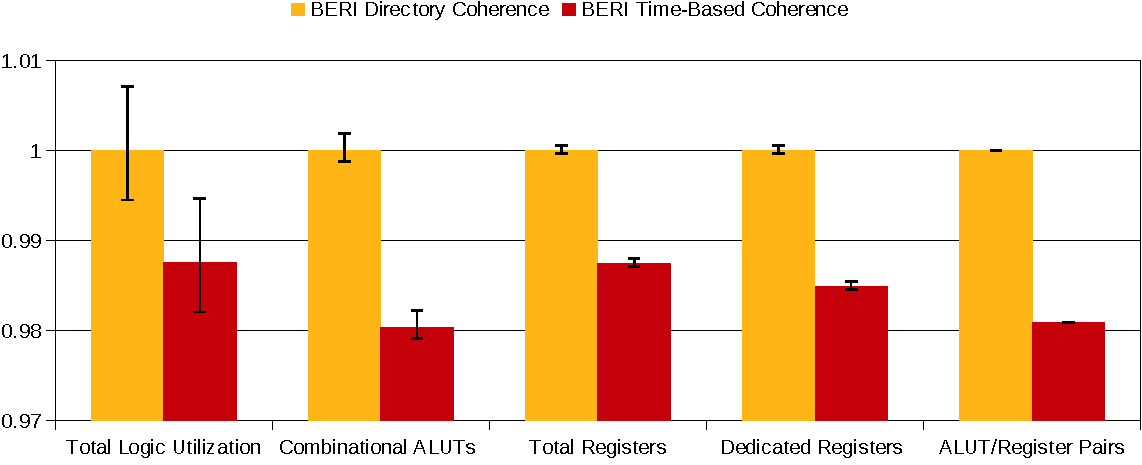
\includegraphics[trim={0 0cm 0 0cm},clip,width=\textwidth,height=\textheight,keepaspectratio]{quartus_graph}}
			\caption[Normalised Quartus overheads]{Normalised Quartus overheads (\textit{Note: The total logic utilization is derived from a complete FPGA design synthesis. Registers and ALUTs show CPU overheads})} 
			\label{quartus_graph}
		\end{figure}	
		

\begin{comment}
		\begin{table}[!h]	
		\centering
		\resizebox{\textwidth}{!}{\begin{tabular}{|l||c|c||c|}
			\hline
			\multicolumn{4}{|c|}{Quartus II 64-Bit -- Version 13.1.0} \\
			\multicolumn{4}{|c|}{Family Stratix IV} \\
			\multicolumn{4}{|c|}{Device -- EP4SGX230KF40C2} \\
			\hline
			Statistic & Directory & Time-Based & FPGA Capacity \\
			\hline 
			\hline
			Total Logic Utilization & 105,720 (58\%) & 104,404 (57.2\%) &  182,400 \\
			Combinational ALUTs & 71,723 (39.3\%) & 70,312 (38.5\%) & 182,400 \\
			Total Registers & 65,456 & 64,637 & 14,625,792 \\
			Dedicated Registers & 65,059 & 64,076 & 14,625,792 \\
			Total BRAM Bits & 3,833,174 & 3,796,310 & 14,625,792 \\
			ALUT/Register Pairs & 101,134 & 99,205 & --- \\
			%\hline
			%Total combinational functions & 71,329 & 69,934 & ? \\
			%-- 7 input functions & 1,206 & 1,209 & ? \\
			%-- 6 input functions & 20,908 & 20,417 & ? \\
			%-- 5 input functions & 13,225 & 13,955 & ? \\
			%-- 4 input functions & 12,113 & 11,996 & ? \\
			%-- <=3 input functions & 23,877 & 22,357 & ? \\
			Clustering Difficulty & Low & Low & NA \\
			\hline
		\end{tabular}}
		\caption{Dual-core BERI FPGA Resource Overhead Comparison (Mean)}
		\label{fpga_other_overheads}
		\end{table}
\end{comment}

\clearpage
\section{Application of Time-Based Coherence }
	\label{section_application_timebased}
	So far I have highlighted the properties of time-based coherence. A major advantage of the time-based model is its implementation simplicity, design modularity and lower hardware overheads.
	
	\paragraph{Simplicity}
		This model can be implemented in designs where a dedicated coherence network is undesirable. Any drawbacks of cache self-invalidation may outweigh the design complexity of a message based coherence protocol. 
			
	\paragraph{Usability}
		This model is supported by the widely used FreeBSD operating system. The protocol could be adapted for other operating systems supporting weak consistency, such as Debian GNU/Linux \cite{Merrill03}.
	
	\paragraph{Scalability}
		The multiprocessor evaluation of time-based coherence has been limited by the FPGA size. However, the obtained results permit some speculation. The minimum requirement for the time-based protocol would be some form of consistency in the shared memory/network. Coherence is implemented directly in the private caches, thus, no additional network or communication is required and cores can be plugged directly into the shared fabric. 
		Optimisations such as detection of polling operations and more sophisticated versions may eliminate timestamps all together, leading to a SYNC-only based design.
		
		This coherence scheme could be implemented on small clusters of general purpose cores, sharing a common memory. For instance, tiled chip-multiprocessors.
		Some relevant examples are: (1) MasPar MP-1 \cite{maspar90}, a good example of early work on building multiprocessors. This design consists of multiple processor boards communicating through a network. Each board contains a cluster of cores. (2) The Intel 48-core SCC \cite{Mattson10} processor is based on a tiled design, where each tile holds a pair of processor cores. The two cores can communicate using time-based coherence, while other protocols can be applied to the rest of the network. (3) The Godson-3 processor \cite{godson3} consists of interconnected nodes. Each node contains 4 cores, sharing a bank of L2 caches. Time-based coherence can be used within a node.

		The coherence protocol can be applied to systems with persistent memory, where time-based self-invalidation would work in tandem with requirements to selectively flush data to persistent storage. HP's `The Machine' project \cite{hp_the_machine} is one such example. Coherence support for this system is currently absent and a simple time-based approach could be beneficial.



















%CHAPTER **************************************************************************
%CHAPTER **************************************************************************
%CHAPTER **************************************************************************
%CHAPTER **************************************************************************
%CHAPTER **************************************************************************

\chapter{Memory Consistency Verification}
\label{chapter_validation}

		Litmus tests are an emerging way for architects to evaluate the memory consistency model of a given processor architecture; demonstrated by Alglave et al. \cite{Alglave11}. These tests typically consist of very short parallel memory operations spread over multiple cores, designed to identify subtle variations in memory consistency. Tests evaluate all permutations for a given set of memory instructions. 
		%The AXE test suite \cite{AXE_checker,bluecheck} is a collection of Litmus style tests executed recursively with injection of additional memory instructions. 
		
		The BERI multiprocessor designs are analysed using the AXE memory checking tool in a triple-core set-up, increasing the interleaving of memory operations. 
		This set-up improves the robustness of model evaluation, while also permitting reasonably short simulation times. The AXE observations are further backed by CHERI Litmus tests, designed by Matthew Naylor \cite{CHERI_litmus}. 
		%The performance of the time-based and directory-based designs is evaluated in simulation using Litmus tests (Section \ref{litmus_perfromance}).
		
		In this chapter I will discuss the memory consistency behaviour of time-based coherence, followed by an analysis of the directory-based model, and conclude with a simple performance evaluation using the aforementioned tools.


\section{Verifying BERI Time-Based Coherence}
		The unique behaviour of time-based coherence differentiates it from other relaxed memory models. While systems such as PowerPC state a number of memory consistency properties, not all of these may be visible in hardware. This is due to variations in cache design, memory latency, reordering of instructions, cache optimisations, and many other factors.
		
		In this section I discuss a small selection of interesting observable, non-observable, and forbidden time-based consistency scenarios. The examples use the memory format previously described in Section \ref{mem_format}.

\clearpage
		\subsection{Observable Relaxed Behaviour}
		In this section we look at several relaxed memory consistency scenarios observed on BERI time-based coherence but not observed on the PowerPC memory model. 
		There are many more observable examples but only a few are shown.
		The PowerPC model is illustrated in work by Sarkar et al. and Maranget et al. \cite{Sarkar11,Maranget12}.
		Note that the notion of threads and cores is equivalent for all examples shown in this section.
		%Other scenarios where the PowerPC model and time-based model exhibit similar behaviour are also shown.
		
%Example
%\newpage						
\paragraph{Test (MP+sync+dep)}
		%This example is observable on the time-based model but not on PowerPC \cite{Sarkar11,Maranget12}. 
		Time-based coherence allows stale data to reside in the cache, thus loads to stale memory are allowed. The example shown in Figure \ref{mp_sync_dep_diagram} demonstrates the stated behaviour.
		
		Steps \textbf{(a:)} and \textbf{(b:)} on Thread 0 are both store operations, the former is propagated using the SYNC instruction. The stores update values of \textbf{(x)} and \textbf{(y)} respectively. Thread 1 at step \textbf{(c:)} is dependent on the store at \textbf{(b:)}. The final operation at \textbf{(d:)} is the load of \textbf{(x)}, and loading the initial value is acceptable.
		
		If we assume a sequential memory behaviour with no stale data caching, then the load of \textbf{(x)} at \textbf{(d:)} would always produce an updated value. For our time-based system, the load at \textbf{(d:)} can produce either the original or the updated value of \textbf{(x)}. 
		A valid tag-time-stamp would allow the initial value to reside in the local cache.
		%since the original value can be held in the private cache with a valid tag-time-stamp.

\begin{figure}[!h]
\begin{tcolorbox}[
colback=green!1!white,
colframe=green!75!black]
\begin{center}
\begin{BVerbatim}
*  Memory Operations  *
0: M[0] := 1
0: sync
0: M[1] := 1
1: M[1] == 1 (blocking)
1: M[0] == 0
\end{BVerbatim}
\end{center}		
%\caption{MP+sync+dep.axe}
%\label{mp_sync_dep_instructions}

\centering
\begin{tabular}{|c|c|c|}
\hline
po: program order & dep: dependency (blocking) & rf: read from \\
\hline
\end{tabular}
\vspace{-9mm}

\begin{displaymath}
	\xymatrix{
		Thread \ 0 & \ \ \ \ \ \  & Thread \ 1 \\
		a: W[x] = 1 \ar[d]_{po} & & c: R[y] = 1 \ar[dd]^{dep} \\
		sync \ar[d]_{po} & \ \ \ \ar@2{~>}[dr]^{rf} & \\
		b: W[y] = 1 \ar@/^/@{->}[uurr]^{rf} & & d: R[x] = 0
	}
\end{displaymath}
\end{tcolorbox}
\caption{Test (MP+sync+dep)}
\label{mp_sync_dep_diagram}
\end{figure}

\clearpage
		Step \textbf{(c:)} may produce an updated value, since its data copy could have expired in the private cache. Systems relying on coherence messages may not exhibit this behaviour, since eager coherence messaging will evict stale memory locations. However, systems using lazy coherence messaging along with message reordering might produce a similar outcome.

%Example
%\newpage
\paragraph{Test (WRC+sync+dep)}
		%This example is observable on the time-based model but not on PowerPC. 
		
		Figure \ref{wrc_sync_dep_diagram} shows a triple thread Litmus test evaluating coherence locality, since local core clusters may exhibit stronger consistency than the whole system. 
		
		Thread 0 performs a store to \textbf{(x)} at \textbf{(a:)}, which is observed by Thread 1 at \textbf{(b:)}. Thread 1 proceeds to execute a SYNC instruction followed by a store to \textbf{(y)} at \textbf{(c:)}. The conditions between steps \textbf{(c:)}, \textbf{(d:)} and \textbf{(e:)} are identical to the previous example (MP+sync+dep). As we have already observed, when the load of \textbf{(y)} at \textbf{(d:)} yields the latest value, load of \textbf{(x)} at \textbf{(e:)} may still produce stale data. This test shows that Thread 1 observes the memory operation of Thread 0, but Thread 2 does not, despite a flat core layout. This test can be extended to more than three threads while demonstrating the same outcome.
		
\begin{figure}[!h]
\begin{tcolorbox}[
colback=green!1!white,
colframe=green!75!black]
\begin{center}
\begin{BVerbatim}
*  Memory Operations  *
0: M[0] := 1
1: M[0] == 1
1: sync
1: M[1] := 1
2: M[1] == 1 (blocking)
2: M[0] == 0
\end{BVerbatim}
\end{center}
%\caption{WRC+sync+dep.axe}
%\label{wrc_sync_dep_instructions}

\vspace{1mm}

\begin{displaymath}
	\xymatrix{
		Thread \ 0 & \ \ \ \ \ \  & Thread \ 1  & \ \ \ \ \ \  & Thread \ 2\\
		a: W[x] = 1 \ar@/^/@{->}[rr]^{po} & & b: R[x] = 1 \ar[d]_{po} & & d: R[y] = 1 \ar[dd]^{dep} \\
		& & sync \ar[d]_{po} & \ \ \ \ar@2{~>}[dr]^{rf} & \\
		& & c: W[y] = 1 \ar@/^/@{->}[uurr]^{rf} & & e: R[x] = 0
	}
\end{displaymath}
\end{tcolorbox}
\caption{Test (WRC+sync+dep)}
\label{wrc_sync_dep_diagram}
\end{figure}


%Example
\clearpage	
\paragraph{Test (W+RWC+sync+dep+sync)}
		%This example is observable on the time-based model but not on PowerPC.
		Figure \ref{w_rwc_sync_dep_diagram}, shows an example where two threads can observe each others memory operations, but without explicit dependencies other threads may not. 
		
		Thread 0 performs two store operations at \textbf{(a:)} and \textbf{(b:)}, the former enforced through a SYNC. Thread 1 performs two loads at \textbf{(c:)} and \textbf{(d:)}, enforced through a dependency. The interaction between Threads 0 and 1 is allowed and expected under BERI time-based coherence. Thread 2 performs a store at \textbf{(e:)}, enforced by a sync and followed by a load of \textbf{(x)} at \textbf{(f:)}.
		
		Thread 2 is not explicitly dependant on any operations performed by either Thread 0 or 1, and it is free to load the stale value of \textbf{(x)} from its private cache. Additionally, Threads 0 and 1 do not explicitly depend on Thread 2.
		
		This example highlights the behaviour of clustered processor architectures, where closely located cores may display different consistency behaviour to those far apart.
		The example previously shown in Figure \ref{wrc_sync_dep_diagram} [Test (WRC+sync+dep)] demonstrates a similar core clustering behaviour using a different set of dependencies. 

\begin{figure}[!h]
\begin{tcolorbox}[
colback=green!1!white,
colframe=green!75!black]
\begin{center}
\begin{BVerbatim}
*  Memory Operations  *
0: M[0] := 1
0: sync
0: M[1] := 1
1: M[1] == 1 (blocking)
1: M[2] == 0
2: M[2] := 1
2: sync
2: M[0] == 0
\end{BVerbatim}
\end{center}
%\caption{W+RWC+sync+dep+sync.axe}
%\label{w_rwc_sync_dep_instructions}

\vspace{1mm}

\begin{displaymath}
	\xymatrix{
		Thread \ 0 & \ \ \ \ \ \  & Thread \ 1  & \ \ \ \ \ \  & Thread \ 2\\
		a: W[x] = 1 \ar[d]_{po} & & c: R[y] = 1 \ar[dd]^{dep} & & e: W[z] = 1 \ar[d]^{po} \\
		sync \ar[d]_{po} & & & \ \ \ \ar@2{~>}[dr]^{rf} & sync \ar[d]^{po} \\
		b: W[y] = 1 \ar@/^/@{->}[uurr]^{rf} & & d: R[z] = 0 & & f: R[x] = 0
	}
\end{displaymath}
\end{tcolorbox}
\caption{Test (W+RWC+sync+dep+sync)}
\label{w_rwc_sync_dep_diagram}
\end{figure}

\clearpage
	\subsection{Non-Observable Relaxed Behaviour}
		Relaxed memory consistency without dependencies allows a range of memory behaviours. This example is one of several behaviours allowed by RMO{\large$^\star$} but not displayed by BERI time-based coherence.
%Example
\paragraph{Test (LB+sync+dep)}
		Figure \ref{lb_sync_dep_diagram} shows a cyclic dependency between all memory operations. While blocking instructions are largely implementation dependent, SYNC instructions must provide stronger ordering guarantees. SYNC must guarantee that all preceding memory operations (specifically stores) have been completed. Note that SYNC instructions only apply to the executing thread, they are not expected to propagate memory operations from other threads. 
		
		In this example, \textbf{(b:)} occurs after a SYNC operation, thus it cannot complete before \textbf{(a:)} is observed. Step \textbf{(c:)} is a blocking operation depending on the outcome of \textbf{(b:)}, so \textbf{(d:)} cannot happen before \textbf{(c:)}. Step \textbf{(a:)} expects an update from \textbf{(d:)} and cannot succeed without it.
		
		While RMO{\large$^\star$} allows this behaviour, the BERI memory subsystem cannot produce this ordering outcome.
		It is difficult to suggest a hardware design that would exhibit this behaviour; removing the dependency at \textbf{(c:)} would make it possible. 
		

\begin{figure}[!h]
\begin{tcolorbox}[
colback=orange!1!white,
colframe=orange!75!white]
\begin{center}
\begin{BVerbatim}
*  Memory Operations  *
0: M[0] == 1
0: sync
0: M[1] := 1
1: M[1] == 1 (blocking)
1: M[0] := 1
\end{BVerbatim}
\end{center}

\vspace{1mm}

\begin{displaymath}
	\xymatrix{
		Thread \ 0 & \ \ \ \ \ \  & Thread \ 1 \\
		a: R[x] = 1 \ar[d]_{po} & & c: R[y] = 1 \ar[dd]^{dep} \\
		sync \ar[d]_{po} & & \\
		b: W[y] = 1 \ar@/^/@{->}[uurr] & & d: W[x] = 1 \ar@/_/@{->}[uull]^{rf}
	}
\end{displaymath}
\end{tcolorbox}
\caption{Test (LB+sync+dep)}
\label{lb_sync_dep_diagram}
\end{figure}

\clearpage
		\subsection{Forbidden Behaviour} 
		So far I have shown evidence that the time-based memory model is relaxed and exhibits more relaxed behaviour than some commercial hardware \cite{Maranget12}. The next example demonstrates that this coherence model can still provide strong programmer assurances.

%\newpage
\paragraph{Test (MP+syncs)}
		Figure \ref{mp_sync_diagram} shows that adequate use of SYNC instructions is sufficient for correct software behaviour. In this example, individual threads perform operations enforced through SYNCs. 
		
		Thread 0 updates values of \textbf{(x)} and \textbf{(y)} at \textbf{(a:)} and \textbf{(b:)}, and Thread 1 loads \textbf{(x)} and \textbf{(y)} at \textbf{(c:)} and \textbf{(d:)}. If Thread 1 observes the updated value of \textbf{(y)} then it will also observe the updated value of \textbf{(x)}, the SYNC instruction will guarantee stale data eviction from private caches (\textit{figure shows memory observations that would result in test failure}). 
		Software written for relaxed consistency systems heavily relies on the behaviour demonstrated in this test, FreeBSD uses this communication style. 
		Each SYNC instruction causes an L1 cache flush, and BERI L1 caches are write-through, so the Thread 0 SYNC is actually unnecessary and can be removed.
		%so overusing it is not recommended.
		
\begin{figure}[!h]
\begin{tcolorbox}[
colback=red!1!white,
colframe=red!85!black]
\begin{center}
\begin{BVerbatim}
*  Memory Operations  *
     0: M[0] := 1
     0: sync
     0: M[1] := 1
     1: M[1] == 1
     1: sync
     1: M[0] == 0
\end{BVerbatim}
\end{center}
%\caption{MP+syncs.axe}
%\label{mp_sync_instructions}

\vspace{2mm}

\begin{displaymath}
	\xymatrix{
		Thread \ 0 & \ \ \ \ \ \  & Thread \ 1 \\
		a: W[x] = 1 \ar[d]_{po} & & c: R[y] = 1 \ar[d]^{po} \\
		sync \ar[d]_{po} & \ \ \ \ar@2{~>}[dr]^{rf} & sync \ar[d]^{po} \\
		b: W[y] = 1 \ar@/^/@{->}[uurr]^{rf} & & d: R[x] = 0
	}
\end{displaymath}
\end{tcolorbox}
\caption{Test (MP+syncs)}
\label{mp_sync_diagram}
\end{figure}


\clearpage
% % % % % % % % % % % % % % % % % % % % % % % % % % % % % % % % % % % % % % % % % %
	\subsection{CHERI Litmus Tests}
		\label{cheri_litmus_tests}
		Litmus tests are a way of testing whether specific concurrent behaviours are actually observable in hardware. Unlike the AXE evaluation, which tests the memory subsystem hardware in isolation, these are assembley-language (software) tests that run on the CPU. CHERI Litmus \cite{CHERI_litmus} is a tool that takes a Litmus test and turns it into a software program that repeatedly (1) randomises the variable locations, (2) synchronises the cores, (3) inserts random delays, (4) executes the Litmus test, (5) checks the Litmus test condition, and (6) records the results.
		
		Message passing (MP) with SYNCs has already been presented in Figure \ref{mp_sync_dep_diagram} [Test (MP+sync+dep)], a similar scenario is demonstrated in this section using CHERI Litmus. We observe different memory consistency behaviour depending on the use of SYNCs. The default Litmus MP test does not use SYNC instructions. Lack of SYNCs and a long self-invalidation time-out will ensure that stores from other threads will not be observed. 
		
		Three tests are evaluated: MP1-default, MP1-SYNC, and MP2. Two versions of the MP1 test were created in order to observe all outcomes. The barrier implementation required by the test also plays a major role. The MP2 test uses a SYNC instruction between the two load operations of thread 1, this test mimics the example shown in Figure \ref{mp_sync_diagram} [Test (MP+syncs)]. Time-based coherence guarantees that the specified outcomes will not be observed.

\begin{figure}[t]
\begin{tcolorbox}[
colback=blue!1!white,
colframe=blue!65!black]
\begin{center}
% {0:r2=x; 0:r4=y; 1:r2=x; 1:r4=y;}
\begin{BVerbatim}
        Initial Conditions       
(r2 = address x; r4 = address y;)
Test Condition (1:r3=1 /\ 1:r1=0)

         P0              P1 
1:  li r1,1      |  lb  r3,0(r4) 
2:  sb r1,0(r2)  |  lb  r1,0(r2) 
3:  sb r1,0(r4)  |
4:  sync*        |
\end{BVerbatim} 
\end{center}
\end{tcolorbox}
\caption[Message passing 1, default and modified tests]{Message passing 1, default and modified tests (*optional)}
\label{mp_1_litmus}
\end{figure}

\begin{figure}[!h]
\begin{tcolorbox}[
colback=blue!1!white,
colframe=blue!65!black]
\begin{center}
%{0:r2=x; 0:r4=y; 1:r2=x; 1:r4=y;}
\begin{BVerbatim}
        Initial Conditions       
(r2 = address x; r4 = address y;)
Test Condition (1:r3=1 /\ 1:r1=0)

         P0              P1 
1:  li r1,1      |  lb  r3,0(r4) 
2:  sb r1,0(r2)  |  sync 
3:  sync         |  lb  r1,0(r2) 
4:  sb r1,0(r4)  | 
\end{BVerbatim}
\end{center}
\end{tcolorbox}
\caption{Message passing 2, default test}
\label{mp_2_litmus}
\end{figure}

		Figure \ref{mp_1_litmus} shows the code sequence used in the MP1 test. The default test is executed without the SYNC instruction (line 4). In the modified test, the SYNC instruction in added into the sequence. Figure \ref{mp_2_litmus} shows the MP2 test. The two SYNC instructions (P0: line 3 and P1: line 2), ensure that this condition is never observed on time-based coherence.

		The barrier loop implemented in CHERI Litmus is shown in Figure \ref{barrier_litmus}. The SYNC instruction (line 6) is not present in the default case. 
		This instruction has been added to observe the desired memory states and to improve the overall execution time on the time-based model. 
		The barrier contains two loops: one is dependant on LL/SC instructions, and the second relies on shared memory updates. 
		
		This code uses a polling technique to wait for memory updates. Lines will be locally cached until the timer expires, and depending on the time-out, this loop could take a long time to execute. The SYNC instruction ensures that fresh data copies are fetched more frequently.
		
		If SYNC instructions are omitted, the time-based model with a simple polling detection mechanism can be used, it speeds-up overall performance while maintaining the correct consistency model.
		
\begin{figure}[!h]
\begin{tcolorbox}[
colback=violet!1!white,
colframe=violet!75!black]
\begin{center}
\begin{BVerbatim}
1:  lld    $8, 0(%0)  < :: :: :: ::
2:  daddu  $8, $8, %1            ::
3:  scd    $8, 0(%0)             ::
4:  beqz   $8, 1b     {Branch to 1}
5:  nop
6:  sync*             < :: :: :: ::
7:  ld     $8, 0(%0)             ::
8:  bne    $8, %2, 6b {Branch to 6}
9:  nop
10: sync
\end{BVerbatim} 
\end{center}
\end{tcolorbox}
\caption{Barrier implementation}
\label{barrier_litmus}
\end{figure}
		
\begin{table}[!ht]
\centering
\resizebox{\textwidth}{!}{\begin{tabular}{c|c|c|l|c|c|c|c|}
\cline{2-8} 
& Modified & Polling & \multicolumn{1}{|c|}{Coherence} & \multicolumn{4}{ c| }{Observed Outcomes} \\ 
\cline{5-8}
& Barrier & Detection & \multicolumn{1}{|c|}{Model} & r3=1 & r3=0 & r3=0 & r3=1 \\
& & & & r1=1 & r1=1 & r1=0 & r1=0 \\
\hhline{-=======}
\multicolumn{1}{|c }{\multirow{4}{*}{\parbox{1.6cm}{\centering MP1 Default}}} &
\multicolumn{1}{|c|}{} & \multicolumn{1}{|c|}{} & Time-Based & 0 & 0 & \textbf{\textcolor{Bittersweet}{1000}} & 0 \\
\multicolumn{1}{|c }{} &
\multicolumn{1}{|c|}{$\bullet$} & \multicolumn{1}{|c|}{} & Time-Based & 81 & 18 & 895 & \textbf{\textcolor{Fuchsia}{6}} \\
\multicolumn{1}{|c }{} &
\multicolumn{1}{|c|}{} & \multicolumn{1}{|c|}{$\ast$} & Time-Based & 321 & 89 & 582 & \textbf{\textcolor{Fuchsia}{8}} \\
\multicolumn{1}{|c }{} &
%\multicolumn{1}{|c|}{$\bullet$} & Time-Based (poll-detect) & 152 & 34 & 801 & \textbf{13} \\
%\multicolumn{1}{|c }{} &
\multicolumn{1}{|c|}{} & \multicolumn{1}{|c|}{} & Directory & 517 & 107 & 376 & 0 \\
\multicolumn{1}{|c }{} &
\multicolumn{1}{|c|}{$\bullet$} & \multicolumn{1}{|c|}{} & Directory & 620 & 101 & 279 & 0 \\
\hline
\multicolumn{1}{|c }{\multirow{4}{*}{\parbox{1.6cm}{\centering MP1 SYNC}}} &
\multicolumn{1}{|c|}{} & \multicolumn{1}{|c|}{} & Time-Based & 271 & 0 & 729 & 0 \\
\multicolumn{1}{|c }{} &
\multicolumn{1}{|c|}{$\bullet$} & \multicolumn{1}{|c|}{} & Time-Based & 71 & 5 & 913 & \textbf{\textcolor{Fuchsia}{11}} \\
\multicolumn{1}{|c }{} &
\multicolumn{1}{|c|}{} & \multicolumn{1}{|c|}{$\ast$} & Time-Based & 342 & 77 & 576 & \textbf{\textcolor{Fuchsia}{5}} \\
\multicolumn{1}{|c }{} &
%\multicolumn{1}{|c|}{$\bullet$} & Time-Based (poll-detect) & 155 & 40 & 795 & \textbf{10} \\
%\multicolumn{1}{|c }{} &
\multicolumn{1}{|c|}{} & \multicolumn{1}{|c|}{} & Directory & 543 & 72 & 385 & 0 \\
\multicolumn{1}{|c }{} &
\multicolumn{1}{|c|}{$\bullet$} & \multicolumn{1}{|c|}{} & Directory & 623 & 22 & 355 & 0 \\
\hline 
\multicolumn{1}{|c }{\multirow{4}{*}{\parbox{1.6cm}{\centering MP2 Default}}} &
\multicolumn{1}{|c|}{} & \multicolumn{1}{|c|}{} & Time-Based & 49 & 43 & 908 & 0 \\
\multicolumn{1}{|c }{} &
\multicolumn{1}{|c|}{$\bullet$} & \multicolumn{1}{|c|}{} & Time-Based & 95 & 43 & 862 & 0 \\
\multicolumn{1}{|c }{} &
\multicolumn{1}{|c|}{} & \multicolumn{1}{|c|}{$\ast$} & Time-Based & 261 & 297 & 442 & 0 \\
\multicolumn{1}{|c }{} &
%\multicolumn{1}{|c|}{$\bullet$} & Time-Based (poll-detect) & 137 & 117 & 746 & 0 \\
%\multicolumn{1}{|c }{} &
\multicolumn{1}{|c|}{} & \multicolumn{1}{|c|}{} & Directory & 529 & 115 & 356 & 0 \\
\multicolumn{1}{|c }{} &
\multicolumn{1}{|c|}{$\bullet$} & \multicolumn{1}{|c|}{} & Directory & 627 & 124 & 249 & 0 \\
\hline
\end{tabular}}
\caption{Litmus: Message passing, observed outcomes}
\label{litmus_table}
\end{table}	

		The test outcomes for MP1-default, MP1-SYNC and MP2 are documented in Table \ref{litmus_table}. This table shows the outcomes of a 1,000 iterations of the Litmus tests in simulation. A cache line lifetime of 10,000 cache cycles is used to produce the displayed results. It is evident that all combinations of register outcomes are only observed in MP1-default and MP1-SYNC, matching the expected behaviour. 
		
		%The tests are highly timing sensitive and achieving all outcomes required some adjustments, however, no modifications were made to the hardware. 		
		An interesting test outcome is observed when the default MP1 test in executed with the default barrier implementation. The output registers constantly read the initial values, since the time-counter does not expire for the entire duration of this test.
		
		The time-based model with polling detection does not require any additional SYNCs to demonstrate the desired outcome. The barrier loop does not rely on cache line time-outs, as the hardware will detect polling and automatically update the line, improving performance and simplifying the observations.

		The Litmus tests were also executed on the directory version of BERI, the results are presented in the same table. Notably the directory model demonstrates a stronger consistency model and the final output (r3=1, r1=0) is never observed, as expected in TSO behaviour. Majority of time-based coherence results display initial value loads, whereas the directory results show a greater number of fully updated or transitional values.

%\clearpage
	\subsection{AXE Trace Evaluation}
		So far I have discussed the behaviour of time-based coherence using specific memory access patterns. While Litmus testing searches for particular
		small examples of RMO, the AXE tool checks
		arbitrary memory traces for consistency, giving further assurances
		about correctness. AXE is used in a hardware testing
		framework where the memory subsystem can be exercised more thoroughly
		than may be possible via software tests running on the processor. The analysis shows why the time-based coherence model complies with RMO{\large$^\star$} and does not meet the requirements of stronger models. The example traces follow the trace format shown in Section \ref{mem_format}.
		
		When AXE detects a consistency failure, the hardware test framework
		proceeds to reduce the number of instructions, weeding out inconsequential or irrelevant instructions, until the failure is no longer observable. All the minimal examples shown here are a product of this reduction process, as a result, the failing traces display significant time gaps where the
		instructions have been automatically removed.

%\clearpage
		\subsubsection{Sequential Consistency Test}
			The test sequence shown in Trace \ref{sc_test_mem} is an extract of an AXE trace, displaying a violation of the SC model by a software simulation of BERI time-based coherence. 
			
			At time 0, core 0 loads the initial value of variable \textbf{(x)}. In the next cycle, core 1 updates the value of \textbf{(x)}. According to sequential consistency, any core loading the value of \textbf{(x)} in any following cycles must observe the latest store value. After several dead cycles, at time 7, core 1 loads the initial value of \textbf{(y)}. A few cycles later, at time 15, core 0 updates the value of \textbf{(y)}. 
			
			The two memory operations on \textbf{(y)} do not violate any SC properties, instead they are introduced as independent memory instructions between operations on \textbf{(x)}. Finally, at time 21, 20 cycles after the first update of \textbf{(x)}, core 0 loads the initial value, violating SC. The reason for this behaviour is that caching of stale values is permitted by BERI time-based coherence.
			
			\captionsetup[table]{name=Trace}
			\begin{table}[!h]
			\begin{center}
			\fontfamily{pcr}\selectfont
			\begin{tabular}{|r|l|l|}
				\hline
				\textbf{Time} & \textbf{Testing SC model} & \multicolumn{1}{c|}{\textbf{Comments}} \\
				\hline 
				Init & \multicolumn{1}{c|}{x==0, y==0} & \\
				& & \\
				0 & $\gg$ 0: x == 0 & core[0].op(LW,addr[0]) \\	
				1 & $\gg$ 1: x := 1 & core[1].op(SW,addr[0]) \\
				7 & $\gg$ 1: y == 0 & core[1].op(LW,addr[1]) \\
				15 & $\gg$ 0: y := 1 & core[0].op(SW,addr[1]) \\
				21 & $\gg$ \textbf{\textcolor{Red}{0: x == 0}} & core[0].op(LW,addr[0]) \\
				& $\gg$ \textbf{\textcolor{Red}{Failed!}} & \\
				\hline
			\end{tabular}
			\caption{AXE: SC evaluation}
			\label{sc_test_mem}
			\end{center} 
			\end{table}
			\captionsetup[table]{name=Table}

			\begin{comment}
			% Raw
			setAddrMap(< 8,  7,  2,  1>)
			chooseVars(<V 0x6 0xf 0xe 0x0  >)
			2061: core[0].op(LW,'h3)
			2062: core[2].op(SW,'h3)
			2068: core[2].op(LW,'h0)
			2076: core[0].op(SW,'h0)
			2082: core[0].op(LW,'h3)
			0: v0 == 0
			2: v0 := 10
			2: v6 == 0
			0: v6 := 8
			0: v0 == 0
			Failed!
			
			\end{comment}

			SC is a very strong model, rarely enforced by hardware, as it imposes strict ordering on memory operations, implementing this behaviour may be difficult or impractical. Additionally, a strong model does not result in a better cache performance, since every shared data store will likely block all other memory operations, resulting in pipeline stalls.

		\subsubsection{Total Store Order Consistency Test}
			Similar to the SC evaluation, an example of the TSO consistency violation is shown in Trace \ref{tso_test_mem}.
			
			At time 0, core 0 loads the initial value of variable \textbf{(x)}. At time 4, core 1 updates the value of \textbf{(x)}, after a few dead cycles, the same core updates the value of \textbf{(y)} (time 12). At this point both memory locations \textbf{(x)} and \textbf{(y)} have been updated. Loading of stale values from either location is not permitted by SC, however, TSO permits stale loads as long as the ordering of stores has not been violated. 
			
			At time 15, core 0 observes the updated value of \textbf{(y)}, indicating that any stale copies of the variable have been evicted from its privet cache. However, 33 cycles later, at time 48, the same core loads the initial value of \textbf{(x)}, violating TSO. The trace would pass TSO under these circumstances:
			
			\begin{enumerate}
				\item If the final load of \textbf{(x)} preceded the updated load of \textbf{(y)}, the behaviour would satisfy TSO.
				\item If the memory instructions were to be executed in the same sequence, only an updated load of \textbf{(x)} would satisfy TSO.
			\end{enumerate}
			 
			\captionsetup[table]{name=Trace}
			\begin{table}[!h]
			\begin{center}
			\fontfamily{pcr}\selectfont
			\begin{tabular}{|r|l|l|}
				\hline
				\textbf{Time} & \textbf{Testing TSO model} & \multicolumn{1}{c|}{\textbf{Comments}} \\
				\hline 
				Init & \multicolumn{1}{c|}{x==0, y==0} & \\
				& & \\
				0 & $\gg$ 0: x == 0 & core[0].op(LW,addr[0]) \\
				4 & $\gg$ 1: x := 1 & core[1].op(SW,addr[0]) \\
				12 & $\gg$ 1: y := 1 & core[1].op(SW,addr[1]) \\
				15 & $\gg$ \textbf{\textcolor{ForestGreen}{0: y == 1}} & core[0].op(LW,addr[1]) \\
				48 & $\gg$ \textbf{\textcolor{Red}{0: x == 0}} & core[0].op(LW,addr[0]) \\
				& $\gg$ \textbf{\textcolor{Red}{Failed!}} & \\
				\hline
			\end{tabular}
			\caption{AXE: TSO evaluation}
			\label{tso_test_mem}
			\end{center} 
			\end{table}
			\captionsetup[table]{name=Table}
			
			\begin{comment}
			%Raw
			setAddrMap(<10,  8,  6,  0>)
			chooseVars(<V 0x8 0xd 0xa 0xf  >)
			2062: core[0].op(LW,'h0)
			2066: core[2].op(SW,'h0)
			2074: core[2].op(SW,'h2)
			2077: core[0].op(LW,'h2)
			2110: core[0].op(LW,'h0)
			0: v8 == 0
			2: v8 := 10
			2: v10 := 18
			0: v10 == 18
			0: v8 == 0
			Failed!
			\end{comment}

		The TSO model is widely used in multiprocessor architectures. One such example is x86, its memory model has extensive coherence support which allows relatively fast distribution of coherence messages necessary for TSO consistency.

		\subsubsection{Partial Store Order Consistency Test}
			The PSO memory model is designed to account for write buffers. The buffers allow batching of writes to consecutive memory locations, thus reducing traffic to the private caches. This behaviour is also beneficial for write-through caches, since it minimises the number of updates to shared memory. Loading values from write buffers is permitted and useful when software repeatedly updates and reloads data. PSO consistency allows reordering of stores to independent memory locations. BERI does not use write buffers in either of the architectures and the time-based version fails this test due to caching of stale data. Example shown in Trace \ref{pso_test_mem} demonstrates this behaviour. Unlike the SC and TSO scenarios, here we observe memory interactions between three cores.
			
			At time 0, core 2 loads the initial value of variable \textbf{(x)}. After many dead cycles, at time 43, core 1 loads the initial value of \textbf{(y)}. This operation does not have any significance in the final outcome. At time 45, core 0 updates the value of \textbf{(x)}. 2 cycles after the store operation, core 1 observes the updated value of \textbf{(x)}. This is an important result, indicating that the update has been propagated to shared memory (the two operations on variable \textbf{(z)} are not significant). 41 cycles after core 1 observed the update value of \textbf{(x)}, core 2 (time 88) loads the initial value, violating PSO. Identifying a failure of PSO requires more testing cycles than either SC or TSO as its exhibits a more relaxed behaviour.

			\captionsetup[table]{name=Trace}
			\begin{table}[!h]	
			\begin{center}
			\fontfamily{pcr}\selectfont
			\begin{tabular}{|r|l|l|}
				\hline
				\textbf{Time} & \textbf{Testing PSO model} & \multicolumn{1}{c|}{\textbf{Comments}} \\
				\hline 
				Init & \multicolumn{1}{c|}{x==0, y==0} & \\
				& & \\
				0 & $\gg$ 2: x == 0 & core[2].op(LW,addr[0]) \\
				43 & $\gg$ 1: y == 0 & core[1].op(LW,addr[1]) \\
				45 & $\gg$ 0: x := 1 & core[0].op(SW,addr[0]) \\
				47 & $\gg$ 1: x == 1 & core[1].op(LW,addr[0]) \\
				57 & $\gg$ 1: z := 1 & core[1].op(SW,addr[2]) \\
				72 & $\gg$ \textbf{\textcolor{BurntOrange}{2: z == 1}} & core[2].op(LW,addr[2]) \\
				88 & $\gg$ \textbf{\textcolor{Red}{2: x == 0}} & core[2].op(LW,addr[0]) \\
				& $\gg$ \textbf{\textcolor{Red}{Failed!}} & \\
				\hline
			\end{tabular}
			\caption{AXE: PSO evaluation}
			\label{pso_test_mem}
			\end{center} 
			\end{table}
			\captionsetup[table]{name=Table}

						\begin{comment}
						setAddrMap(< 5,  3,  2,  0>)
						chooseVars(<V 0xa 0x1 0x3 0xf  >)
						%2086: core[1].op(LW,'h1)
						2095: core[2].op(LW,'h3)
						2138: core[1].op(LW,'h0)
						2140: core[0].op(SW,'h3)
						2142: core[1].op(LW,'h3)
						2152: core[1].op(SW,'h2)
						2167: core[2].op(LW,'h2)
						2183: core[2].op(LW,'h3)
						%1: v1 == 0
						2: v15 == 0 %x
						1: v10 == 0 %y
						0: v15 := 8 %x
						1: v15 == 8 %x
						1: v3 := 9 %z
						2: v3 == 9 %z
						2: v15 == 0 %x
						Failed!
						\end{comment}
			
			Desired behaviour could be achieved by inserting a SYNC instruction in the core 2 memory sequence just prior to the final load of \textbf{(x)}. It would cause an eviction of stale data and result in an updated load. Synchronisation instructions are the only way of guaranteeing updated shared memory loads.
			
	\subsection{Regression Testing}
		Extensive AXE verification has confirmed that BERI time-based coherence complies
		with the \textbf{RMO{\large$^\star$}} consistency model (\textit{Note: RMO{\large$^\star$} is a subset of the AXE RMO memory model}). The checker tool has analysed 1,000,000 memory instruction permutations on the coherence model in simulation. Table \ref{time_based_regression} shows memory executions with different parameters. The instruction depth indicates the number of instructions checked for correct consistency behaviour. Each instruction depth was tested with a varying set of instructions, 200 times.
		
		Axe supports checking atomicity of successful LL/SC pairs, the memory subsystem can be stimulated with LL/SC operations (+LLSC) in addition to normal loads and stores. Each model parameter can affect system behaviour. The presence of an LL/SC instruction could affect the time between other memory operations. If a SYNC verification step relies on this timing, an incorrect test success may be declared. In order to avoid such a scenario, the time-based memory consistency scheme was tested with all combinations of test parameters.

		\begin{table}[!b]	
		\begin{center}					
		\begin{tabular}{|l||c|c|c|}
			\hline
			Model Parameters & Instruction Depth & No. of Iterations & Outcome \\ 
			\hline 
			RMO & 5000 & 200 & Pass \\
			RMO +LLSC & 5000 & 200 & Pass \\
			RMO +SYNC & 5000 & 200 & Pass \\
			RMO +LLSC +SYNC & 5000 & 200 & Pass \\
			\hline
		\end{tabular}
		\caption{AXE time-based coherence memory consistency verification}
		\label{time_based_regression}
		\end{center} 
		\end{table}

		AXE aggressively tests the memory subsystem. The tool does not account for the processor pipeline, and the rate of memory operations injected into the caches may be impossible to achieve with a full processor. However, this form of testing allows us to provide very strong grantees on memory behaviour since the worst case is tested. The tool is very efficient at spotting inconsistencies, in most cases a memory model failure is detected with an instruction depth of less than 1,000. Larger instructions depths, exceeding 5000 instructions have also been tested, yielding identical results\footnote{The extended AXE trace evaluation has not been presented here, since it does not provide any new information regarding memory consistency behaviour.}.




\section{Verifying BERI Directory Coherence}
	I have already presented some Litmus results for the BERI directory-based coherence model in Section \ref{cheri_litmus_tests}. In this section I describe the AXE trace evaluation and regression testing of this coherence implementation.

	\subsection{AXE Trace Evaluation}
		The BERI directory-based coherence model enforces TSO consistency. This memory model was selected partly due to related research in the field, Elver and Nagarajan \cite{Elver14}, and partly due to the inherent properties of coherence messaging. The coherence network allows fast and efficient distribution of messages, intentionally degrading the performance of this network in order to achieve a weaker model is unnecessary. 

		The BERI directory passes all but the SC consistency check in our test framework. The example shown in Trace \ref{directory_sc_test_mem} demonstrates an SC compliance failure. This test shows an interaction between three cores. 
		
		At time 0, cores 1 and 2 load initial values of \textbf{(x)} and \textbf{(y)}. In the following cycle, all three cores perform updates. Core 0 updates \textbf{(x)} and both cores 1 and 2 update the value of \textbf{(y)}. The two stores are conflicting, and one will overwrite the other in shared memory. Finally at time 8, cores 0 and 1 observe the initial values of \textbf{(x)} and \textbf{(y)}. This behaviour is not valid in SC but perfectly acceptable in TSO. 
		
		The coherence messages generated by the directory are likely in transit or blocked due to busy private caches. All invalidates are delivered to all sharer cores simultaneously, however, at least one private cache might be in a fetch state, waiting for a memory response or performing another blocking operation. This will result in an invalidation delay. In our caches, all responses must be consumed before proceeding, thus cancelling a fetch midway is not possible.

		\captionsetup[table]{name=Trace}
		\begin{table}[!t]
		\begin{center}
		\fontfamily{pcr}\selectfont
		\begin{tabular}{|r|l|l|}
			\hline
			\textbf{Time} & \textbf{Testing SC model} & \multicolumn{1}{c|}{\textbf{Comments}} \\
			\hline 
			Init & \multicolumn{1}{c|}{x==0, y==0} & \\
			& & \\
			0 & $\gg$ 1: x == 0 & core[1].op(LW,addr[0]) \\
			0 & $\gg$ 2: y == 0 & core[2].op(LW,addr[1]) \\
			1 & $\gg$ 0: x := 1 & core[0].op(SW,addr[0]) \\
			1 & $\gg$ 1: y := 1 & core[1].op(SW,addr[1]) \\
			1 & $\gg$ 2: y := 2 & core[2].op(SW,addr[1]) \\
			8 & $\gg$ \textbf{\textcolor{Red}{0: y == 0}} & core[0].op(LW,addr[1]) \\
			8 & $\gg$ \textbf{\textcolor{Red}{1: x == 0}} & core[1].op(LW,addr[0]) \\
			& $\gg$ \textbf{\textcolor{Red}{Failed!}} & \\
			\hline
		\end{tabular}
		\caption{AXE: SC evaluation}
		\label{directory_sc_test_mem}
		\end{center} 
		\end{table}
		\captionsetup[table]{name=Table}

					\begin{comment}
					setAddrMap(<17, 12, 11,  5>)
					chooseVars(<V 0xb 0xf 0x4 0x2  >)
					%2065: core[0].op(SW,'h3)
					2065: core[1].op(LW,'h0)
					2065: core[2].op(LW,'h2)
					2066: core[0].op(SW,'h0)
					2066: core[1].op(SW,'h2)
					2066: core[2].op(SW,'h2)
					2069: core[0].op(LW,'h2)
					2069: core[1].op(LW,'h0)
					%2069: core[2].op(SW,'h3)
					%0: v2 := 8
					1: v11 == 0 %x
					2: v4 == 0 %y
					0: v11 := 16 %x
					1: v4 := 9 %y
					2: v4 := 10 %y
					0: v4 == 0 %y
					1: v11 == 0 %x
					%2: v2 := 18
					Failed!
					\end{comment}

	
	\subsection{Regression Testing}
		The BERI directory coherence model is verified using AXE, just like the time-based model. The final revision of this coherence scheme has passed all of the tests shown in Table \ref{directory_regression}. Each test simulation ran a total of 1,000,000 iterations before declaring a pass. Using the tool, the memory model has been tuned to comply with TSO for all input test parameters. Any uncertainty in delivery of coherence messages presents a challenge for fine tuning the consistency model, as even a small additional delay may result in failure of TSO and even PSO.
		
		\begin{table}[!h]	
		\begin{center}					
		\begin{tabular}{|l||c|c|c|}
			\hline
			Model Parameters & Instruction Depth & No. of Iterations & Outcome \\ 
			\hline 
			TSO & 5000 & 200 & Pass \\
			TSO +LLSC & 5000 & 200 & Pass \\
			TSO +SYNC & 5000 & 200 & Pass \\
			TSO +LLSC +SYNC & 5000 & 200 & Pass \\		
			\hline
		\end{tabular}
		\caption{AXE directory-based coherence memory consistency verification}
		\label{directory_regression}
		\end{center} 
		\end{table}
		\vspace{-10mm}

%\clearpage
\section{Performance Evaluation Using Litmus}
		\label{litmus_perfromance}
		The execution time of CHERI Litmus tests on time-based and directory models has highlighted some key performance differences. The directory model exhibits strong memory consistency, and memory updates are actively propagated, thus, barrier loops require fewer cycles to complete. The time-based model (without polling detection) takes much longer to run the test, since barrier loops spend a long time waiting for private caches to self-invalidate and update memory locations, as a result the execution time compared to the directory is higher. Appropriate SYNC instructions in the barrier greatly improve performance. The time-based model with polling detection overcomes these penalties, since the cache hardware can detect stale loads and force an update from lower levels of memory.

\begin{figure}[t]
\begin{tcolorbox}[
colback=blue!1!white,
colframe=blue!65!black]
\begin{center}
\begin{BVerbatim}
      P0     |      P1 
1:  li* r1,1 |  li*  r2,1
2:  nop      |  nop 
\end{BVerbatim} 
\end{center}
\end{tcolorbox}
\caption{Litmus NOP test}
\label{nop_litmus}
\end{figure}

		A special NOP instruction test was written to evaluate the performance \footnote{The Litmus tests are evaluated on a dual socket Intel$\textregistered$ Xeon$\textregistered$ CPU E5-2667 v2, with 8 physical and 16 logical cores per socket, operating at 3.30GHz, and a total DRAM capacity of 256GB. The tests are compiled with mips-linux-gnu-gcc Debian 4.4.5-8.}
		(Figure \ref{nop_litmus}). Litmus tests require some register evaluation, hence, two initialisation instructions were added (line 1). Note that these instructions do not interact with memory, and any observed slowdown will be due to the barrier implementation used to synchronise test iterations.
		
		The execution time of the time-based model with a time-out value of 10,000 cycles and no barrier SYNC shows a ($>$32$\times$) slowdown as compared to a directory model. Inserting a SYNC instruction (barrier previously shown in Figure \ref{barrier_litmus}) reduces the slowdown to just over (2$\times$). The relative improvement in the execution time of time-based coherence is ($>$14$\times$). 
		
		At least 5 samples were taken for each test and no more than a 1\% variation in the timing samples was observed for all tests. The cycle accurate simulation produced identical results in each run, so the execution time variation can be attributed to OS behaviour. These results are shown in Table \ref{litmus_nop_performance}. 
		
		The strength of the time-based mechanism lies in correctly crafted code. As we will see in Chapter \ref{coherence_eval}, performance of the optimised coherence mechanism is often equivalent and on occasion better than shown by the directory-based model when running FreeBSD. Additional barrier SYNC instructions have no significant effect on the directory model due to an eager coherence behaviour. There is a small penalty for executing the SYNC instruction but it is negligible compared to other test overheads. 
		%The testing environment used for Litmus testing is described in Table \ref{vaucher_system_info}.
		
		The best performance of the time-based model is achieved when using the cache polling detection mechanism. The private cache is able to determine when an address is polled, thus, a stale location is more frequently updated, and execution time is reduced. Without a barrier SYNC, the polling detection mechanism reduces the total execution time to 85 sec, $\sim$6\% slower than the directory model. The small performance penalty observed is due to self-invalidates and SYNC based cache invalidates. Interestingly, the test version with a barrier SYNC performed worse in this case (98 seconds), as the additional SYNC instruction reduces the cache hit rate. Thus, best performance for the time-based model is achieved when the number of SYNCs and polling operations is well balanced.

		The Litmus testing framework only uses memory instructions and branch instructions, any latency added by the memory subsystem appears more significant when compared to regular application where arithmetic operations are more common. This test framework allows careful analysis of memory behaviour and its effect on overall performance.

		\begin{table} %[!h]
		\begin{center}
		\begin{tabular}{|c|c|c|c|}
		\hline
		Coherence & Modified & Polling & Execution \\
		Model & Barrier & Detection & Time (sec) \\
		\hline
		Time-Based & & & 2575 \\
		Time-Based & $\bullet$ & & 180 \\
		Time-Based & & $\ast$ & 85 \\
		Time-Based & $\bullet$ & $\ast$ & 98 \\
		Directory &  & & 80 \\
		Directory & $\bullet$ & & 80 \\
		\hline
		\end{tabular}
		\caption{Litmus NOP test performance}
		\label{litmus_nop_performance}
		\end{center} 
		\end{table}	


\section{Summary}
	In this chapter I have demonstrated that the BERI time-based coherence model complies with the RMO{\large$^\star$} memory consistency scheme, defined in Chapter \ref{chapter_background}. The directory-based coherence scheme is proven to comply with the TSO memory consistency model. I have also evaluated the basic performance of both coherence models in simulation, using the memory checking tools.




















































































































	
	
	
	
	
\begin{comment}
*** 4 Reg Polling Detector
Observed outcomes:
321: 1:r3=1 1:r1=1 
89: 1:r3=0 1:r1=1 
582: 1:r3=0 1:r1=0 
8: 1:r3=1 1:r1=0 
OBSERVED
real	1m25.138s
user	1m24.969s
sys	0m0.072s

*** 4 Reg Polling Detector + barrier SYNC
Observed outcomes:
152: 1:r3=1 1:r1=1 
34: 1:r3=0 1:r1=1 
801: 1:r3=0 1:r1=0 
13: 1:r3=1 1:r1=0 
OBSERVED
real	1m57.938s
user	1m57.805s
sys	0m0.075s

*** 4 Reg Polling + SYNC
Observed outcomes:
342: 1:r3=1 1:r1=1 
77: 1:r3=0 1:r1=1 
576: 1:r3=0 1:r1=0 
5: 1:r3=1 1:r1=0 
OBSERVED
real	1m29.020s
user	1m28.776s
sys	0m0.084s

*** 4 Reg Polling Detector + SYNC + barrier SYNC
Observed outcomes:
155: 1:r3=1 1:r1=1 
40: 1:r3=0 1:r1=1 
795: 1:r3=0 1:r1=0 
10: 1:r3=1 1:r1=0 
OBSERVED
real	1m42.602s
user	1m42.300s
sys	0m0.084s

MP2 + polling
Observed outcomes:
261: 1:r3=1 1:r1=1 
297: 1:r3=0 1:r1=1 
442: 1:r3=0 1:r1=0 
NOT OBSERVED
real	1m28.618s
user	1m28.435s
sys	0m0.089s

MP2 + polling + barrier sync
Observed outcomes:
137: 1:r3=1 1:r1=1 
117: 1:r3=0 1:r1=1 
746: 1:r3=0 1:r1=0 
NOT OBSERVED
real	1m38.830s
user	1m38.629s
sys	0m0.073s
\end{comment}

	
\begin{comment}
\paragraph{\textbf{AXE Test (LB+dep)}}
		This example (Figure \ref{lb_dep_diagram}) shows a cyclic dependency between all memory operations running on hardware threads. Blocking instructions are largely implementation dependent, BERI time-based coherence permits blocking memory operations to proceed (RMO without dependencies).

		In this example, threads attempt to load values of \textbf{(x)} and \textbf{(y)} at steps \textbf{(a:)} and \textbf{(c:)} respectively. Both load operations are blocking and no new memory operations will be issued until the conditions are satisfied. Steps \textbf{(b:)} and \textbf{(d:)} perform stores to \textbf{(y)} and \textbf{(x)} respectively, these values are required by \textbf{(c:)} and \textbf{(a:)}. Blocking instructions will prevent this sequence form succeeding, unless blocking operations are ignored by the memory subsystem and load/store reordering is permitted. The time-based coherence model does not prevent this scenario, however, the cache structure of BERI does not support out of order execution or reordering of memory instructions.

\begin{figure}[!h]
\begin{tcolorbox}[
colback=orange!1!white,
colframe=orange!75!white]
\begin{center}
\begin{BVerbatim}
*  Memory Operations  *
0: M[0] == 1 (blocking)
0: M[1] := 1
1: M[1] == 1 (blocking)
1: M[0] := 1
\end{BVerbatim}
\end{center}
%\caption{LB+dep.axe}
%\label{lb_dep_instructions}
\vspace{5mm}
%\centering

%\begin{tcolorbox}
\centering
\begin{tabular}{|c|c|c|}
\hline
po: program order & dep: dependency(blocking) & rf: read from \\
\hline
\end{tabular}
\begin{displaymath}
\xymatrix{
	Thread \ 0 & \ \ \ \ \ \  & Thread \ 1 \\
	a: R[x] = 1 \ar[dd]_{dep} & & c: R[y] = 1 \ar[dd]^{dep} \\
	& & \\
	b: W[y] = 1 \ar@/^/@{->}[uurr] & & d: W[x] = 1 \ar@/_/@{->}[uull]^{rf}
}
\end{displaymath}
\caption{AXE Test -- LB+dep}
\label{lb_dep_diagram}
\end{tcolorbox}
\end{figure}
\end{comment}	
	
	
\begin{comment}	
\section{NEW BERI DUAL-CORE WITH ENHANCED CACHES AND COHERENCE}
	The revised version of BERI multi-core has several enhancements. Cache enhancements have been largely credited to Jonathan Woodruff and Alexandre Joannou. The modifications have been largely based on the original version of BERI multi-core. I have added a new Coherence Controller module. This module disassociates the directory from the modular cache. This optimisation allows using the same Bluespec cache modules for all versions of caches: I-Cache, data cache, and L2 (Other levels are possible as well). The Coherence Controller is responsible for keeping a track of sharers and issuing invalidates. The specific workings of the shared cache are masked from the Coherence Controller as this module just observes memory accesses and track data sharing.
	
	\begin{itemize}
	\item All the caches are modular with a number of configurable parameters such as: associativity, capacity, prefetching, out of order behaviour, etc.
	\item The Coherence Controller hold both the directory and the LL/SC resisters.
	\item The data caches perform full lookups for each invalidate, provided the congestion is low. During high congestion phases of operation, the cache simply invalidates the address without a lookup.
	\item The SYNC instruction waits for all outstanding writes to complete before releasing the pipeline. 
	\end{itemize}
\end{comment}


% % % % % % % % % % % % % % % % % % % % % % % % % % % % % % % % % % % % % % % % % % %
\begin{comment}
Tests produce the following histograms:
\begin{table}[!h]	
\begin{center}					
\begin{tabular}{c|l|c|c|c|c|c|}
\cline{2-7} 
& & Approx & \multicolumn{4}{ c| }{Observed Outcomes} \\ 
\cline{4-7}
& \multicolumn{1}{|c|}{Coherence Model} & \multicolumn{1}{c|}{Time} & r3=1 & r3=0 & r3=0 & r3=1 \\
& & \multicolumn{1}{|c|}{(sec)} & r1=1 & r1=1 & r1=0 & r1=0 \\
\hhline{-======}
\multicolumn{1}{|c }{\multirow{4}{*}{\parbox{1.6cm}{\centering MP1 default}}} &
\multicolumn{1}{|l|}{Time-Based} & 2575 & 0 & 0 & \textbf{1000} & 0 \\
\multicolumn{1}{|c }{} &
\multicolumn{1}{|l|}{Time-Based \scriptsize{(B-SYNC)}} & 180 & 81 & 18 & 895 & \textbf{6} \\
\multicolumn{1}{|c }{} &
\multicolumn{1}{|l|}{Directory} & 75 & 517 & 107 & 376 & 0 \\
\multicolumn{1}{|c }{} &
\multicolumn{1}{|l|}{Directory \ \ \ \scriptsize{(B-SYNC)}} & 75 & 620 & 101 & 279 & 0 \\
\hline
\multicolumn{1}{|c }{\multirow{4}{*}{\parbox{1.6cm}{\centering MP1 modified}}} &
\multicolumn{1}{|l|}{Time-Based} & 1380 & 271 & 0 & 729 & 0 \\
\multicolumn{1}{|c }{} &
\multicolumn{1}{|l|}{Time-Based \scriptsize{(B-SYNC)}} & 180 & 71 & 5 & 913 & \textbf{11} \\
\multicolumn{1}{|c }{} &
\multicolumn{1}{|l|}{Directory} & 75 & 543 & 72 & 385 & 0 \\
\multicolumn{1}{|c }{} &
\multicolumn{1}{|l|}{Directory \ \ \ \scriptsize{(B-SYNC)}} & 75 & 623 & 22 & 355 & 0 \\
\hline 
\multicolumn{1}{|c }{\multirow{4}{*}{\parbox{1.6cm}{\centering MP2 default}}} &
\multicolumn{1}{|l|}{Time-Based} & 1465 & 49 & 43 & 908 & 0 \\
\multicolumn{1}{|c }{} &
\multicolumn{1}{|l|}{Time-Based \scriptsize{(B-SYNC)}} & 180 & 95 & 43 & 862 & 0 \\
\multicolumn{1}{|c }{} &
\multicolumn{1}{|l|}{Directory} & 75 & 529 & 115 & 356 & 0 \\
\multicolumn{1}{|c }{} &
\multicolumn{1}{|l|}{Directory \ \ \ \scriptsize{(B-SYNC)}} & 75 & 627 & 124 & 249 & 0 \\
\hline
\end{tabular}
\caption{Litmus: Message Passing Observed Outcomes}
%\label{litmus_observations}
\end{center} 
\end{table}	
\end{comment}

% 3 lines below ensure that there is a blank page before a new chapter
\clearpage
\thispagestyle{empty}
\mbox{}
%TODO: SCA
\makeatletter
%\newcommand{\rmnum}[1]{\romannumeral #1 }
%\newcommand{\Rmnum}[1]{\expandafter\@slowromancap\romannumeral #1@}
\makeatother
\ifpdf
\graphicspath{{Chapter2/Chapter2Figs/PNG/}{Chapter2/Chapter2Figs/PDF/}{Chapter2/Chapter2Figs/}}
\else
\graphicspath{{Chapter2/Chapter2Figs/EPS/}{Chapter2/Chapter2Figs/}}
\fi

\chapter{Cache Side-Channel Attacks}
	\label{chapter_sca}

	Timing Side-Channel Attacks (SCAs) rely on measuring cache misses through memory access latency. We hypothesise that cache self-invalidation reduces observable timing variations, thus masking the leakage of side-channel information. In general, SCAs are a method of gathering information through physical observations of a system. The attack does not seek weaknesses in software algorithms (usually cryptographic), instead it relies on the physical properties of the system. Common attacks include: timing analysis, power monitoring, electromagnetic emanations, and many more. 
	
	In this chapter I focus on timing memory operations and extracting useful information correlated with the behaviour of a critical application, the Victim. If the Victim application is a cryptosystem then the analysis of its memory usage may compromise security. AES is a widely used cryptographic algorithm and it is often used as a target in SCA research. Timing attacks on AES have shown successful cryptographic key extraction through cache side-channels \cite{Brumley03,Percival05,Bonneau06_0}. 
	In AES, the key value and the plain text affect the memory usage of the algorithm. Profiling the memory usage will allow an estimation of the key with a high degree of certainty. 
	
	Extraction of security critical information through side-channels is well understood; I will focus primarily on reducing cache side-channel leakage rather than key extraction or data decryption.

\section{Effects of Coherence on SCAs}
	Coherence mechanisms such as snooping or directories are designed to provide shared memory communication. These schemes focus on efficient shared memory updates and do not actively conceal any memory latency variations. Compared to a single processor system, a multiprocessor should provide no additional SCA protection other than misdirection through parallel software execution. SCAs work best when the attacking code and the Victim code are collocated (operating on the same processing element or memory segment). Successful attacks are possible even when the applications are not collocated, information can be extracted by timing shared or main memory accesses \cite{Ristenpart09,Brumley11,Hund13,Yarom14}.
	
	I have established the behaviour of time-based coherence in previous chapters. The scheme  ejects cached data at regular intervals, thus, adding timing entropy and masking some of the cache side-channel leakage. This system property is inherent and does not require any additional support. SCA mitigation can be further improved by making some minor software modifications.

\section{SCAs on BERI/CHERI}
	\textcolor{red}{The CHERI architecture is designed to provide fine grained memory protection. Capabilities allow fixed memory segment allocation for each application. Allocated memory segment are exclusive to each process. This mechanism provides robust protection against software attacks such as buffer overflows. However, the capability model does not protect against SCAs.}

	\textcolor{red}{Capabilities provide memory bounds for application data. This data is stored in memory just like any other data. Capabilities enforce memory address bounds, but they do not directly affect cached data. Capabilities themselves are stored in memory but tagged with an additional bit to differentiate them from non-capability data.}

	\textcolor{red}{Cache SCAs attempt to determine the memory usage of a particular application and thereby uncover the operations performed. As far as a spy program is concerned, the memory data usage of a capability-protected application and a traditionally compiled application is similar. Major differences will be linked to capability memory operations and any additional memory required for storing capabilities. Capabilities do not replace paging, so any SCAs designed to exploit TLB paging will remain effective. If a cryptographic algorithm is executed on a capability system, it will be safe against memory leaks but not against SCAs.}

	\subsection{Cryptography and SCAs}
		The behaviour of a cryptographic algorithm is dependant on the input data, key, or often both. A variation in any one of the parameters will usually result in different cryptographic steps. Encryption algorithms such as RSA, ElGamal, and Digital Signature Algorithm use modular exponentiation in one of the steps \cite{Daly02}. This operation calculates the remainder (z) when as integer (x) is raised to the power (p) and divided by a positive integer (y). This algorithm is iterative and the input parameters will affect memory usage. The memory usage can diverge to the extent that keys can be delivered from coarse side-channel memory behaviour observations.
	
	\subsection{State of the art SCA Mitigation}
		A number of SCA mitigation techniques have already been mentioned in Chapter \ref{chapter_background}. They can be broadly grouped into four categories: 
		
		\begin{enumerate}
			\item OS-driven mitigation techniques such as removal of caching privileges, cache flushing, and skewing timing device measurements.
			\item Algorithm specific masking modifies the behaviour of a cryptographic algorithm. In case of AES, the memory footprint of each encryption round can be kept constant. Loading the entire s-box into the cache would ensure uniform access.
			\item Dedicated hardware modules for popular cryptographic schemes can be added to commercial systems. These dedicated accelerators bypass the caches altogether.
			\item Modified cache behaviour can improve the level of side-channel masking. Techniques such as cache partitioning, pseudo-random or random cache misses, and non-deterministic prefetching.
		\end{enumerate}
	
	\subsection{Exploiting Time-Based Coherence for SCA Mitigation}
		Traditional cache coherence mechanisms are designed for parallel performance and memory consistency. The addition of a coherence scheme affects memory behaviour by adding a level of indirection.
		
		The time-based cache coherence mechanism is simple to implement in the context of BERI architecture. A side-effect of self-invalidating private caches is a subtle masking of an applications memory footprint. The level of mitigation provided for collocated Attacker-Victim applications may be equivalent to the applications running on completely independent cores.
		
		The coherence model is not very effective at mitigating attacks aimed at lower levels of memory, such as the shared cache or main memory. However, aggressive self-invalidation adds noise to time measurements when attacking the lower levels. This uncertainty can be overcome through higher SCA sampling. 
	
\section{BERI SCA Analysis}
	Modern processor designs incorporate multi-tired caches with a diverse behaviour, making side-channel attacks much more difficult, as demonstrated by Mowery et al. \cite{Mowery12}. The BERI memory subsystem is fairly simple compared to commercial designs. Direct mapped caches, in-order execution, no write buffers, no memory access reordering, simple prefetching, and other factors make BERI highly susceptible to SCAs. The BERI platform is ideal for SCA mitigation analysis as the memory architecture does not mask side-channels. Direct mapped caches ensure interference between the Victim and Trojan (attacker) data, this interference is less certain in set-associative caches. In-order execution and no memory reordering ensures a sequential attack.

	\subsection{Memory Footprint Analysis}
		Information leakage of a memory system is best quantified through a controlled experiment that does not rely on cryptographic algorithms. Attacks usually described in SCA research focus on cryptographic properties that may not be applicable to other programs. AES attacks include: One-Round, Two-Round, Evict+Time, Prime+Probe, and others \cite{Osvik06}. 
		
		The first two attacks are directly aimed at AES, whereas the other two can be applied to general applications. The Prime+Probe attack is one of the stronger options. An attacker plants some Trojan code in the desired system. The objective is to interfere with cache behaviour and thereby extract useful side-channel information. This style of attack has been tested on both directory and time-based coherence protocols; in simulation with no OS and on FPGA whilst running FreeBSD.
		
		The Prime+Probe attack can be applied on a varying scale, from a single memory location to an entire cache. Coarse grained timing measurements and a generally noisy system might force the attacker to use a single cache line attack. Figure \ref{prime_and_probe} shows an example of a Prime+Probe attack. In order to simplify the explanation, let us assume that the cache only holds 4 lines and the Victim application requires only 1 cache line for its data. The SCA steps are listed below:
		
		\begin{figure}[!h]
		\centering 
			\makebox{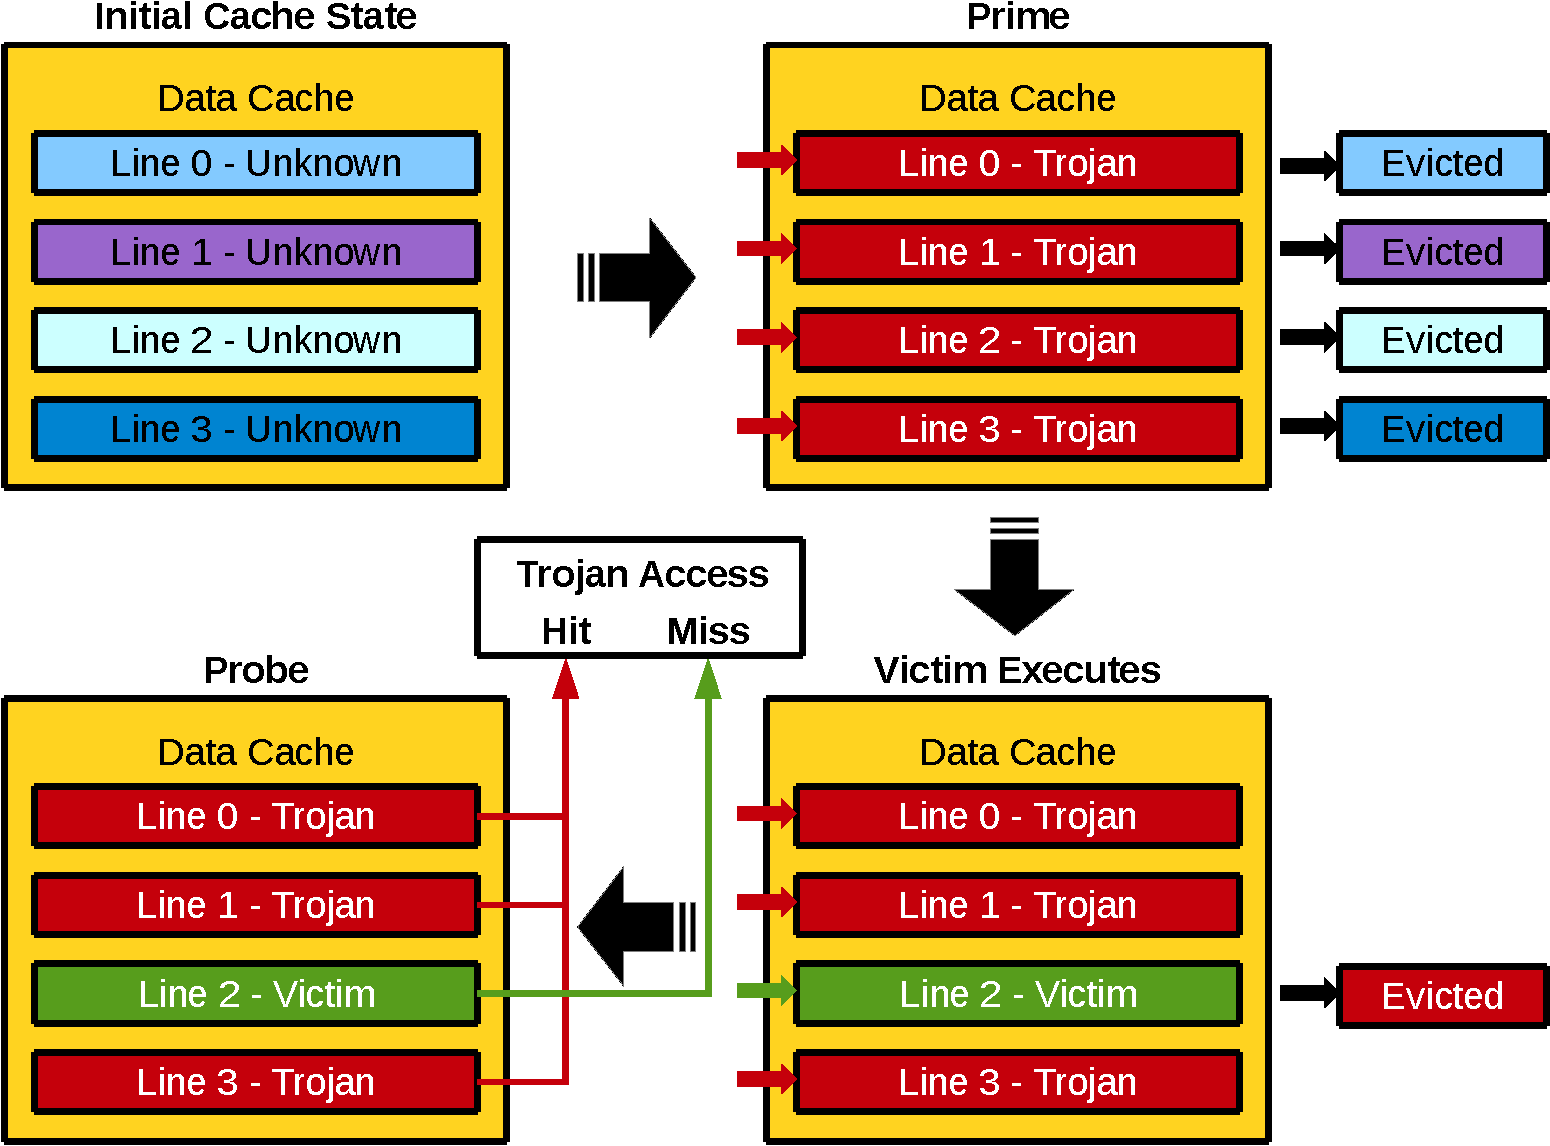
\includegraphics[width=\textwidth,height=\textheight,keepaspectratio]{prime_and_probe}}
			\caption{Prime+Probe attack} 
			\label{prime_and_probe}
		\end{figure}
		%\vspace{-5mm}
		
		\begin{enumerate}
			\item Initial Cache State: At this point the cache is in an unknown state, likely holding unrelated or invalid data.
			\item Prime: The Trojan begins by loading its own data into every line of this cache (4 memory lines in this example).
			\item Victim Executes: The Victim application is allowed to execute. In this example the application uses line 2 of the cache to hold its data. Thus, data previously held in line 2 is evicted (Trojans data).
			\item Probe: The Trojan measures memory latency by reading back its own data from memory, any misses in the cache will add latency, hardware time counters or OS counters can be used. Since line 2 has been evicted, the Trojan will be able to determine that an application executed prior to the Probe phase accessed line 2.
		\end{enumerate}
		
		The example shown is very simple but when it is scaled up to a full system, the Trojan will be able to determine the memory footprint of the Victim application. In the case of AES, this would allow an attacker to recursively work out the cryptographic key used for a certain piece of data. The same attack principle can be applied to a variety of applications, but most mitigation techniques only focus on cryptographic algorithms.

	\subsection{Effects of Coherence on SCAs}
		Multi-threaded applications can benefit from some masking effects produced by cache coherence. Any invalidations or updates through a coherence network can cause cache performance variations, making accurate side-channel measurements more challenging. If the Trojan application is run synchronously with the Victim, the programs may not be collocated. Thus, to observe Victim behaviour the Trojan requests will need to access shared memory. In this discussion I will mostly focus on single threaded applications in order to simplify the analysis. 
		
		\subsubsection{Directory Coherence -- SCA}
			This coherence protocol is designed to efficiently cache most frequently used data, update stale memory lines, and eliminate false sharing. The Prime+Probe attack relies on evictions caused by the cache usage of a critical application with the Probe phase revealing the memory usage.
			
			%\textcolor{red}{I have found that under appropriate OS testing conditions a multiprocessor system might be more vulnerable to SCAs, compared to a uniprocessor. The OS exploits the multi-threaded nature of the multiprocessor architectures to distribute workloads and achieve higher efficiency. Thus, other cores can As a result, the probe measurements contain less noise; generated by other processes, interrupts, exceptions, etc. These results are further illustrated in Section \ref{os_prime_probe_attack}.}
			
			The complex memory architecture of a multiprocessor systems often adds a layer of SCA indirection. However, multi-threading may still benefit an attacker. When the Trojan and Victim applications are executed on the same CPU, remaining cores can handle the OS and other processes. A uniprocessor system may add more noise to the Trojan timing results, due to interference from other processes. I have tested SCAs in a very controlled environment which showed more consistent results on the directory-based system. These results are further illustrated in Section \ref{os_prime_probe_attack}.
		
		\subsubsection{Time-Based Coherence -- SCA}	
			This coherence protocol adds unpredictability to cache behaviour by default. The protocol evicts data based on a set lifespan, clearing any stale data. Increasing the miss rate of a cache is not usually desirable, but when dealing with side channels, memory entropy could be beneficial.
			
			The Prime+Probe attack relies on controlled cache data eviction; random memory purging will not yield desired timing information. This is precisely what a time-based coherent system is able to achieve. When the attacker loads data into the cache during the Prime phase, each memory line is assigned a maximum lifespan. When this value is exceeded, the line is evicted. If sufficient time passes between the Prime and Probe phases, the Probe stage will observe data misses and no hits in the private cache. Thus, the coherence mechanism is introducing some SCA mitigation. The coherence mechanism will also have a low performance impact on the critical application (depends on the selected time-out).
			
			Another beneficial trick in favour of time-based coherence is the behaviour of SYNC instructions. As previously mentioned in Section \ref{sync_behaviour}, these instructions ensure that all memory operations prior to SYNC have completed, and all data has been marked invalid. The later is an excellent SCA mitigation mechanism since it acts as a single instruction flush. If a SYNC is used before or preferably after the critical application, it ensures that any Trojan data that might be in the cache is evicted. Importantly, SYNC will also evict all data belonging to the critical application (Figure \ref{prime_and_probe_time_based}). 
			
			\begin{figure}[t]
			\centering 
				\makebox{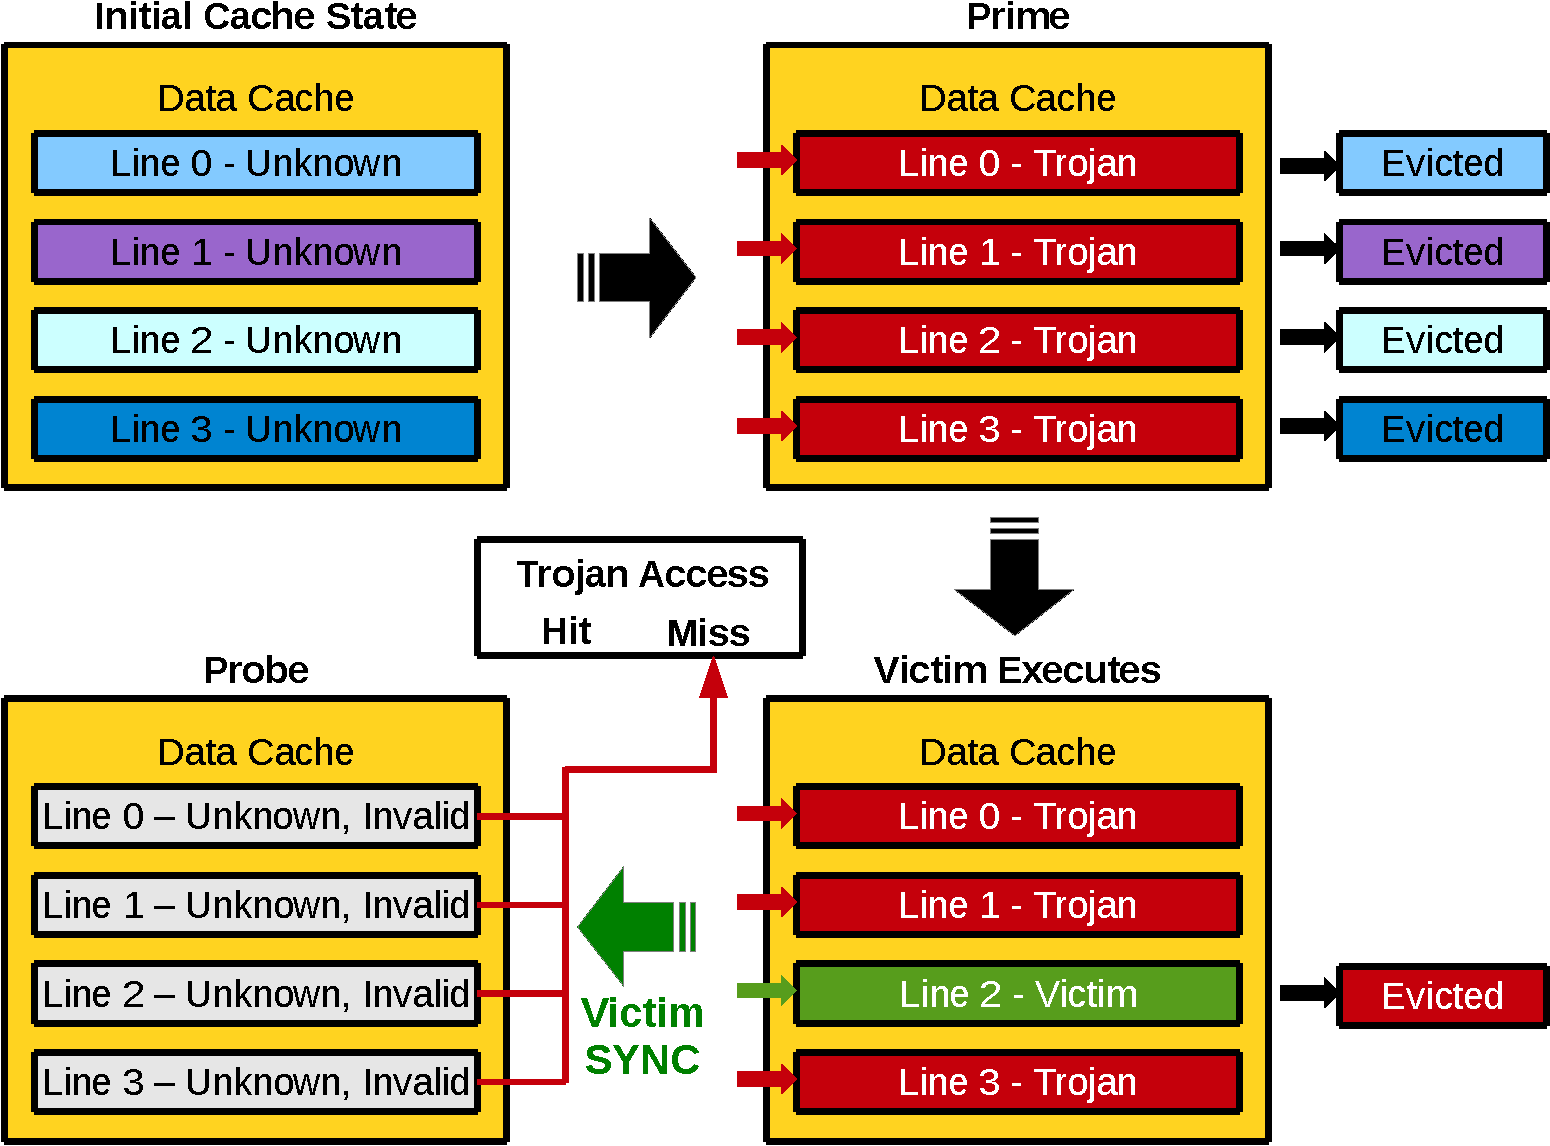
\includegraphics[width=\textwidth,height=\textheight,keepaspectratio]{prime_and_probe_time_based}}
				\caption{Prime+Probe attack, time-based coherence} 
				\label{prime_and_probe_time_based}
			\end{figure}
			%\vspace{-5mm}
			
			I have previously mentioned that time-based coherence does little to mitigate attacks on lower levels of memory, such as the shared cache. However, incorporating the single cycle flush mechanism may help. The shared cache tends to be much larger than the private caches, so purging cached data may degrade overall performance. These overheads could be reduced by flushing data only when the Victim application completes or during a context switch. Systems using three levels of cache could benefit from this mechanism at levels 1 and 2, but level 3 cache purging may be too costly. Attacks on level 3 caches have been demonstrated and SCA protection at this level will likely require one of the techniques suggested in \cite{Irazoqui15,Yarom14,Hund13,Brumley11}.
	
	\section{Experimental Set-up}
		In this section evaluate the level of SCA mitigation provided by time-based coherence. The memory footprint of a simple application is estimated through a cache side-channel. In order to simplify the analysis of the timing data and remove any unexpected noise due to other data in the cache, the  critical application or Victim is a simple loop containing memory load and store operations. Test simplicity and lack of external factors, greatly improve chances of a successful SCA. 
		
		The Trojan program consists of two array manipulation loops: Prime and Probe. The Prime loop loads a data cache sized array and stores it repeatedly in a volatile variable. This ensures that the operation is not optimised away by the compiler. The loaded value is updated and stored back into the cache. The Probe phase simply loads all previously ``primed'' data and measures the execution time of the loop. Any fluctuations in total time will reveal the hit-miss ratio. The Prime+Probe attack is applied to the entire BERI data cache (16KB, 32 bytes per line, 512 lines). The test yields very precise results in a controlled bare metal Bluesim environment. 

		%\textcolor{red}{However, when testing with an OS, such a measurement style suffers from noise due to other programs. Testing under FreeBSD on FPGA yields far more erratic results, but more timing samples allow us to conduct a successful SCA.} 
		SCA testing on FreeBSD OS is noisier and requires more Probe samples, I do not block other processes or interrupts during the test. The main test objective is to establish any SCA masking effects provided by the cache, so the same level of time sampling is applied to all designs under tests.
		
		\begin{enumerate}
			\item Prime: The Trojan populates the entire data cache with its data.
			\item Victim: The Victim program is allowed to execute. This program loads and stores chunks of memory. The size of this memory can be adjusted. A larger chunk of memory would result in more Trojan data evictions from the data cache.
			\item Probe: The Trojan loads all of its data and measures the execution time of the loop.
		\end{enumerate}
		
		The BERI data cache used in this evaluation is 16KB in size with 32 bytes per line. In order to reduce the execution time of the Trojan, the program only loads and stores every 32\textsuperscript{nd} byte of its memory chunk. This ensures that each data cache line will contain at least one byte of Trojan data. The exact placement of the Trojan byte within the line is irrelevant, as any other memory access to this line will cause a miss due to mismatched Tags, resulting in Trojan data eviction.
		
		This test also operates at the granularity of an L2 cache; the Trojan populates the shared cache but the Victim dataset is still limited to the L1 data cache size. In most cases the best Trojan timing information is extracted when only the data cache is populated. Time-based coherence provides no protection for the shared cache since it has no control over L2 evictions. Side channel attacks on shared caches are discussed further in Section \ref{protecting_llc}.
	
	\section{Bare Metal Testing}
		In the bare metal environment (\textit{i.e.} no OS) we have access to all hardware counters that may be restricted to kernel space. Counters are read through coprocessor 0 (CP0) using the read hardware register (RDHWR) instruction. The data cache counters are fed into CP0 every cycle. Counters used in this evaluation are:
		
			\begin{itemize}
				\item \textbf{Time:} This counter follows the standard MIPS model and provides a cycle-accurate count.
				\item \textbf{Miss:} Total data cache misses, including both loads and stores.
				\item \textbf{Hit:} Total data cache hits, including both loads and stores.
			\end{itemize}
	
		\subsection{Collocated Tests}
			Multiprocessor systems allow application parallelism, an important consideration when it comes to memory side-channel evaluation. Many SCAs rely on the Trojan and the Victim application to be collocated, that is, sharing the same private cache. This test evaluates an SCA on a Victim application where both are executed on the same core. On BERI, the Trojan and Victim codes are tied to core 0. Core affinity is assured by locking Core 1 in an infinite loop, so that minimal interference is expected.

\begin{comment}
\url{Location: /home/aam53/TestsForMIPSResults/BaremetalTestResults/20151106_baremetal_core_pin/*}
\end{comment}

			\subsubsection{Results}
				The Victim code operates on a dataset with a memory size ranging from 0 bytes to a maximum of 16,384 bytes (maximum data cache capacity). The memory usage of the Victim is increased every test iteration in order to determine the amount of side-channel leakage. The test gathers the following processor statistics for each memory test size: (1) Trojan Probe time, (2) Trojan Probe miss count, (3) Trojan Probe hit rate, and (4) Victim execution time.
				
				\paragraph{Expected Behaviour}
					The initial cache state is irrelevant, so the Trojan begins the Prime phase by reading in uninitialised data and updating it to a known value. The Trojan is only interested in timing measurements but initialising the data is useful for debugging. BERI data caches are non write-allocate, loads ensure subsequent caching of stores. Each cache line holds 32 bytes of data and it is sufficient for the Trojan to only touch every 32\textsuperscript{nd} byte of its data. A total of 512 loads and 512 stores are performed in the Prime phase.
					
					Following the Prime operation, core 0 begins executing the Victim code. This code consecutively loads bytes, increments their value, and then stores them back into the cache. The load operation is sufficient to evict a Trojan line but the increment operation is added to simulate some kind of useful work. It isn't a memory operation so it simply passes through the pipeline, spacing out memory accesses.
					
					Once the Victim completes its execution, the Trojan begins the Probe phase. Counter values are acquired and stored in specific memory locations. The Trojan performs 512 load operations. Any data not present in the data cache will result in a miss and an access to the L2 or main memory, this generates additional latency and a slower execution of the Probe phase. 
					On completion, the counters are read again and the difference between initial and final values provide the required information. Note that several unrelated memory accesses due to counter loading are acknowledged in the final count, the added error is minuscule and does not show a significant impact on the overall results.
					
					The Victim dataset size is determined through time-counter values and reinforced by other counters. Timing data gathered by the Trojan can precisely identify the Victims memory footprint. Timing results are also supported by capturing hit and miss counters, thus verifying Trojan and Victim behaviour.
				
				\paragraph{Observed Behaviour - Single-Core}
					In the bare metal environment, the single-core Trojan and Victim behaviour is almost identical to that shown by the directory. The absence of a coherence network reduces any coherence noise that may be present in the directory version. Given the similarity in observations, we will discuss these in the directory section below.
				
				\paragraph{Observed Behaviour - Directory}
					As expected in a processor with no side-channel mitigation and Trojan-Victim collocation, the Probe observations are highly deterministic and perfectly correlate with variations in the Victim's dataset size. 
					The size is directly proportional to the execution time and miss rates of the Trojan Probe phase, the hit rate of Trojan Probe data is inversely proportional to the Victim dataset size. 
					No data sharing is expected, so any coherence messages observed in the cache are due to L2 cache capacity misses. Trojan observations are limited to the line granularity of the cache. BERI caches use 32 bytes per line, any Victim dataset variations below that threshold are non-observable.
					
					The normalised 2D cross-correlation function in Matlab calculates the correlation coefficients of the two inputs; the array of Victim datasets and the array of Trojan Probe execution times. The result shows a sharp peak centred around 1 where the two data sequences show maximum correlation.
				
				\paragraph{Observed Behaviour - Time-Based}
					%\textcolor{red}{Trojan observations are dramatically different in the time-based system. The Probe phase execution time and hit/miss rates are very noisy. Additionally the miss rate is much higher since the Trojan data has been self-invalidated from the data cache. The hit rate is equally chaotic. The correlation chart shown no peaks since there is no correlation between the Trojan time data and the Victim dataset size.}
					
					The Trojan Probe samples little to no correlation with the Victims dataset size. Some side-channel leakage is observable when the Victim execution time is low, however, the obtained results are insufficient for accurately identifying the Victims memory usage. The miss and hit counts are very different to those shown by the single-core or dual-core directory systems. While some similarity is visible, the number of matching samples is low. The timing charts shown in this section may be visually deceptive as some samples overlap, the cross-correlation charts show a more accurate data representation.
				
			\subsubsection{Evaluation}
				Data gathered from the SCA simulation test is shown and discussed in this section. Each cluster of plots is discussed separately.
			
				\paragraph{Figure \ref{baremetal_core_pin_std_1} --}
					The data presented in this figure shows the relation between the Victim process and any side-channel data extracted by the Trojan application. 
					\begin{description}
					\item [a(1,2,3)] 
						We observe a linear relation between the execution time of the Victim application and its dataset size for all three models. Crucially, time-based coherence behaviour for the Victim application is nearly identical. Thus, any side-channel masking offered by time-based coherence does not negatively impact the Victim application.
					\item [b(1,2,3)] 
						When we zoom in to the a(1,2,3) data, we see that single-core and dual-core directory models display identical Victim behaviour. Time-based coherence b(3) follows the same general pattern with occasional high latency samples due to time-counter roll-overs in the L1 data cache. Approximately 11\% of all Victim executions suffer from these performance penalties.
					\item [c(1,2,3)] 
						This chart analyses latency experienced by the Trojan Probe for each Victim dataset size. The single-core and directory designs both show a linear relationship between the two chart parameters. This result follows the expected behaviour of a system lacking SCA protection. The Victim test code does not use any software SCA mitigation techniques such as cache flushing, uncached accesses, etc.
						
						Trojan Probe execution measurements are dramatically different in the time-based results, the Trojan experiences almost no data cache hits and even shows L2 cache misses. The Victim program runtime affects the total time between the Prime and Probe stages, since time-based coherence self-invalidates data at fixed times, a greater Victim runtime results in a lower Trojan hit rate. This test shows that the Probe phase does not provide any meaningful results even at low Victim execution times. The time-based model used in this test has a fixed time offset value of 10,000 cycles. Once the execution time of the Victim exceeds 10,000 cycles, the data cache no longer holds any valid Trojan data. 
						%Lower execution times result in some side-channel leakage that is more visible in the next chart described below.
					\item [d(1,2,3)] 
						Looking at a region of charts c(1) and c(2) produces the patterns shown in d(1) and d(2). While data in c(1) and c(2) appears as a straight line, in reality the time values form more of a staircase pattern. Each step shows 32 identical time samples values followed by a jump to a new time value. This is due to bytes per line timing granularity, since 32 data bytes are located within a cache line. The Trojan can only observe latency at a line granularity. Both dual-core directory and single-core show identical behaviour.
						
						The time-based model shows a high fluctuation in latency. The staircase pattern is not observable in this data. The time-based model displays a much greater overall latency (y-axis minimum and maximum) in this window. Note that the high rate of variation in the Trojan measurement is present even for very small Victim execution times, and even when there is no Victim data. The Trojan Prime phase takes a certain amount of time to complete, and by the time it has finished, some of the lines written at the beginning might be near the end of their lifespan. For this reason, the Trojan might experience high memory latency even at low Victim execution rates.
					\end{description}
				
				\paragraph{Figure \ref{baremetal_core_pin_std_2x} --}
					In this chart we look at the cache hit, miss and correlations for the Trojan-Victim test.
					\begin{description}
					\item [a(1,2,3)] 
						The single-core and dual-core directory models follow the same pattern. The number of cache hits decreases proportionally with the increase in Victims dataset size. This behaviour is expected judging by the timing data displayed in the previous chart. 
						The Minimum cache hit of 0 is observed when the Victim fills the entire cache (16384 bytes) and the maximum cache hit of 512 is achieved when the Victims dataset size is 0. The Trojan only requires 512 memory accesses to touch every data cache line. 
						
						The time-based model shows an erratic cache hit behaviour. The number of hits is variable and often near 0 even when the Victim size is 0 (time-counter roll-overs may occur during the Prime phase). Hits significantly reduce once the Victim size exceeds the time-counter roll over threshold, 4 bit counter with a 10,000 cycle timing offset, a total of 160,000 cycles. Note that each memory operations will require multiple cycles to complete. In the previous Figure \ref{baremetal_core_pin_std_1}, charts a(1,2,3) show that the Victims execution time exceeds 160,000 cycles 
						\footnote{The time-counter continues incrementing through the Trojan Prime phase, and these cycles must be added to the Victims execution time. For this reason the sharp drop in Probe hit rate is observed when the Victims dataset size is at $\sim$11,000.}
						when the dataset size is $\sim$12,000. This directly translates to the sudden drop in hit rate experienced by the time-based model in a(3).
					\item [b(1,2,3)] 
						Miss count for all charts is inversely proportional to the corresponding hit rate, discussed above. This property holds for the entire range of the Victim dataset.
					\item [c(1,2,3)] 
						Data presented so far has shown a clear distinction between different model behaviours. Correlations between the Victim and Trojan results are easy to visualise. However, if the Victim dataset size is randomly varied, it may be more difficult to visually identify correlations. Hence, data presented in charts c(1,2,3) and d(1,2,3) quantifies the results using a normalised cross-correlation function. This technique should consistently identify any correlation between the Victim and Trojan behaviour. The single-core and directory correlations are identical as the input data is effectively the same. We see a strong peak where the cross-correlation of the Victims dataset size and Trojans Probe timing yields maximum similarity. The time-based model shows no correlation whatsoever.
					\item [d(1,2,3)]
						Here we look at the cross-correlation between the acquired hit and miss counts for all the models. Since cache hit and miss counts are inversely proportional for both single-core and directory, a strong inverse peak is observed. A minor correlation is also observable in the time-based data comparison. If the cache miss/hit data were to be available to an attacker, useful information could still be extracted when using the time-based model.
					\end{description}

% Figure batch 1
					\begin{figure}[!h]
					\centering 
						\makebox{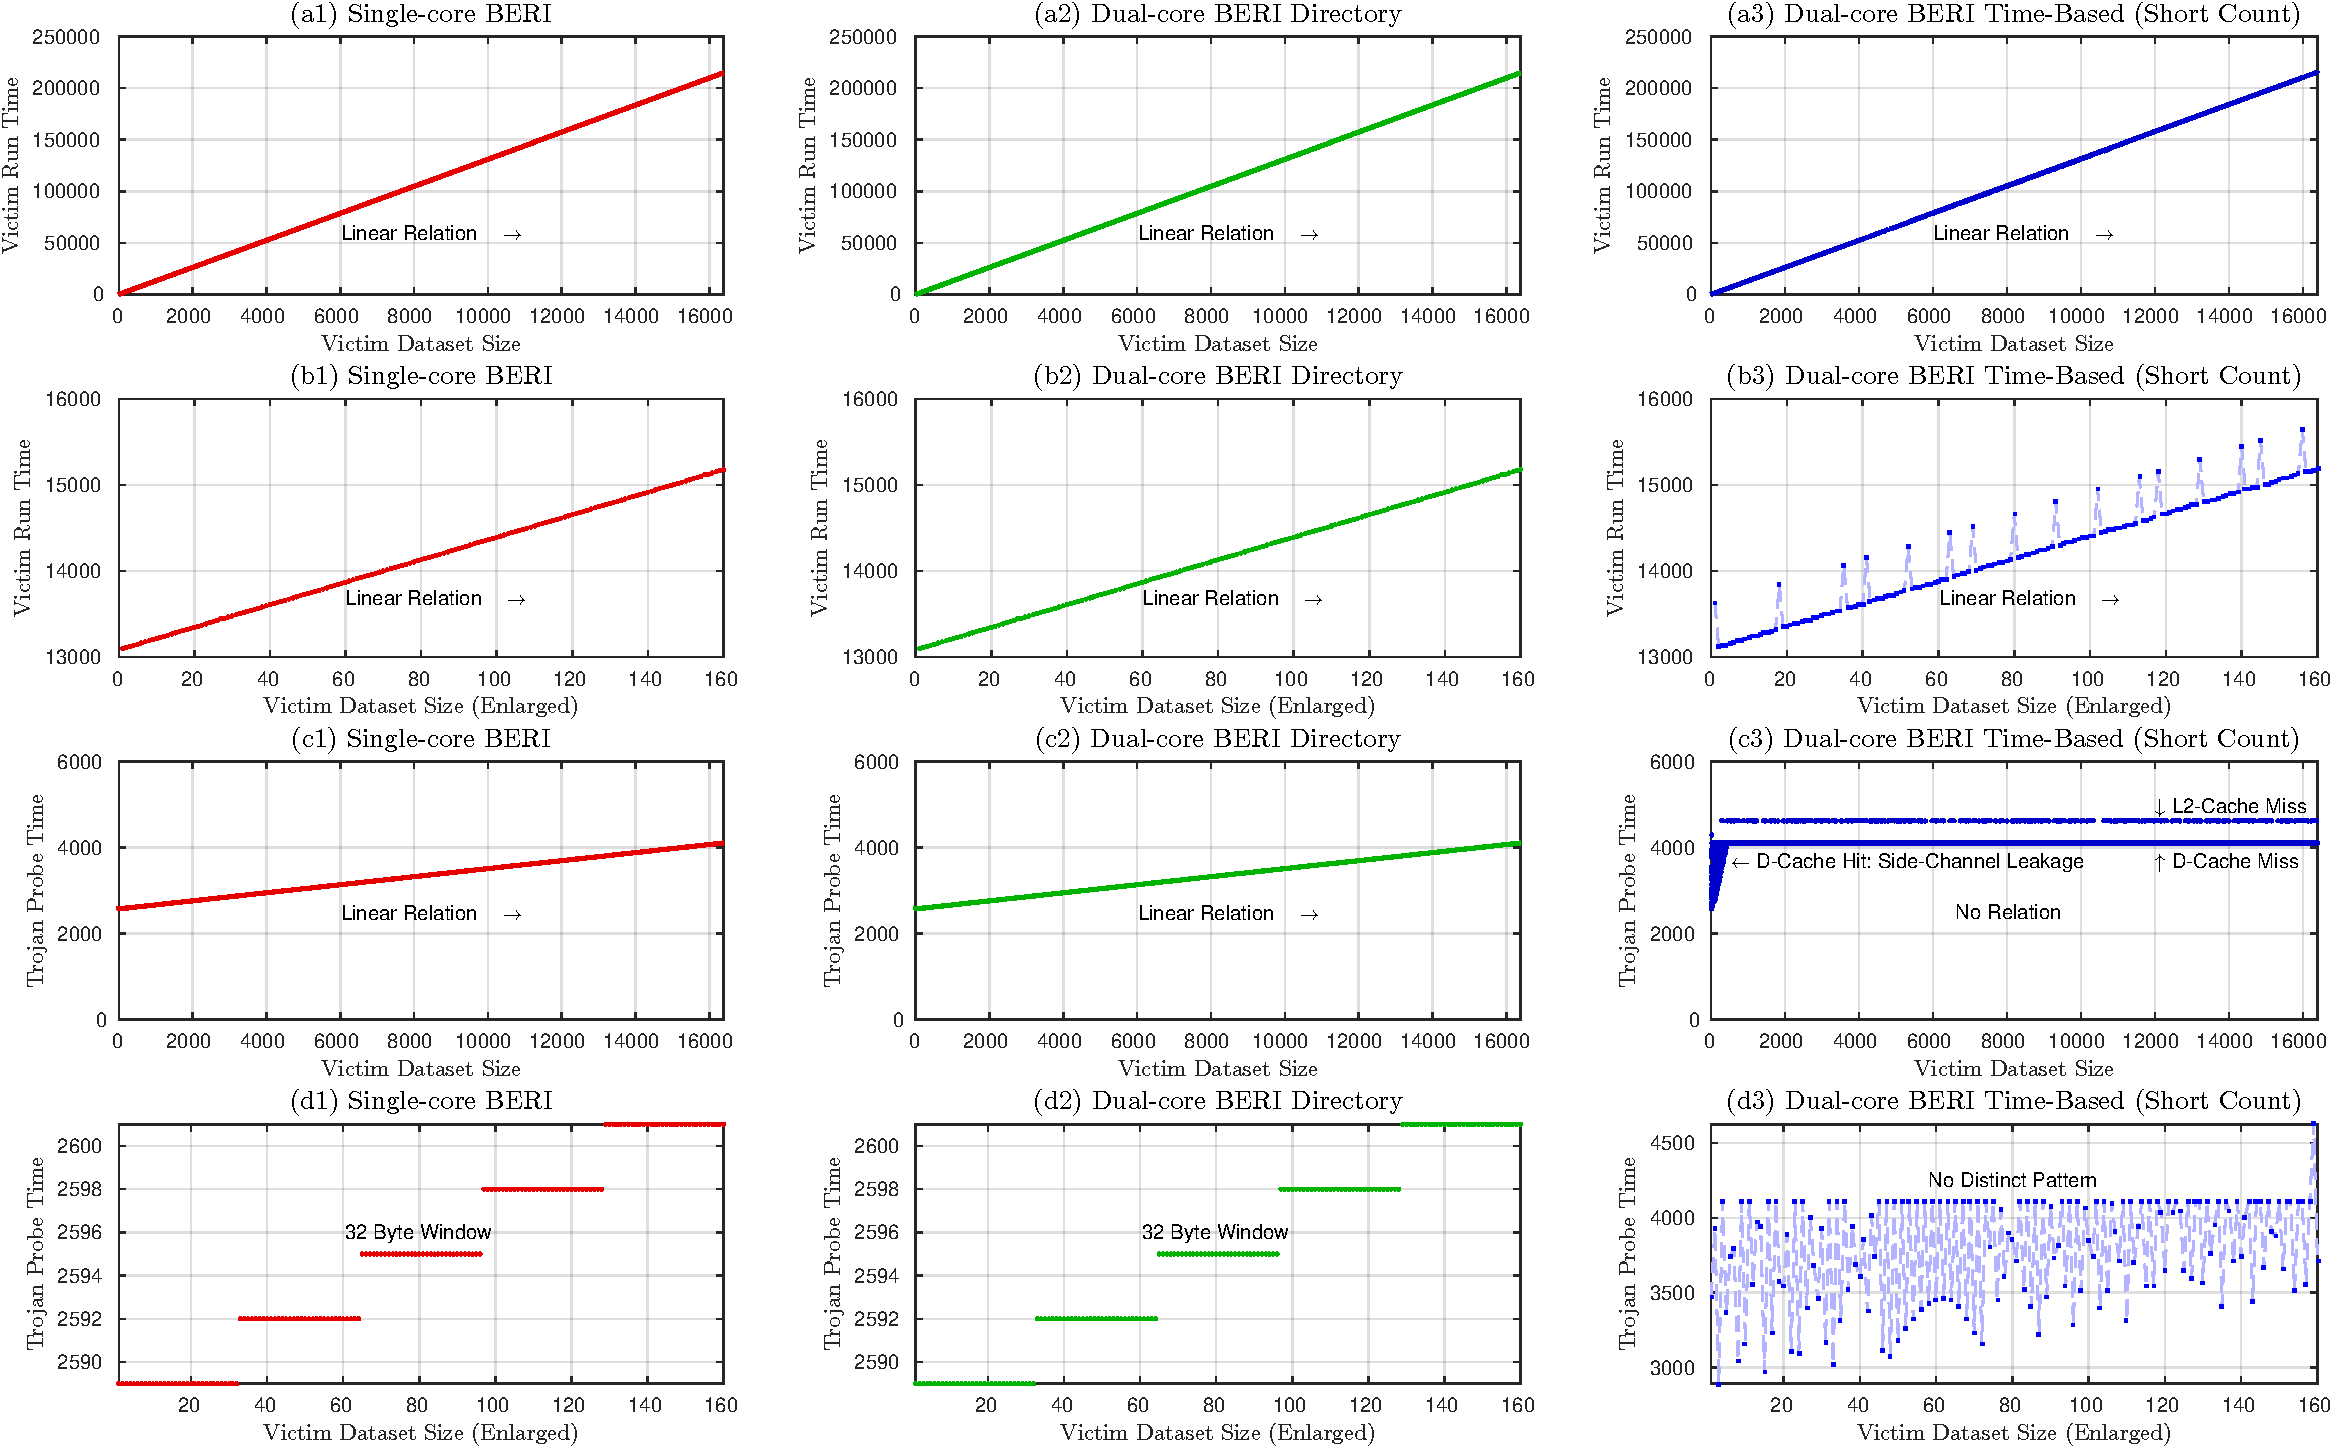
\includegraphics[width=\textheight,height=0.95\textwidth,keepaspectratio,angle=90]{sca_baremetal_standard_1}}
						\caption{Bare metal side-channel attack, chart (1a)} 
						\label{baremetal_core_pin_std_1}
					\end{figure}
					
					\begin{figure}[!h]
					\centering 
						\makebox{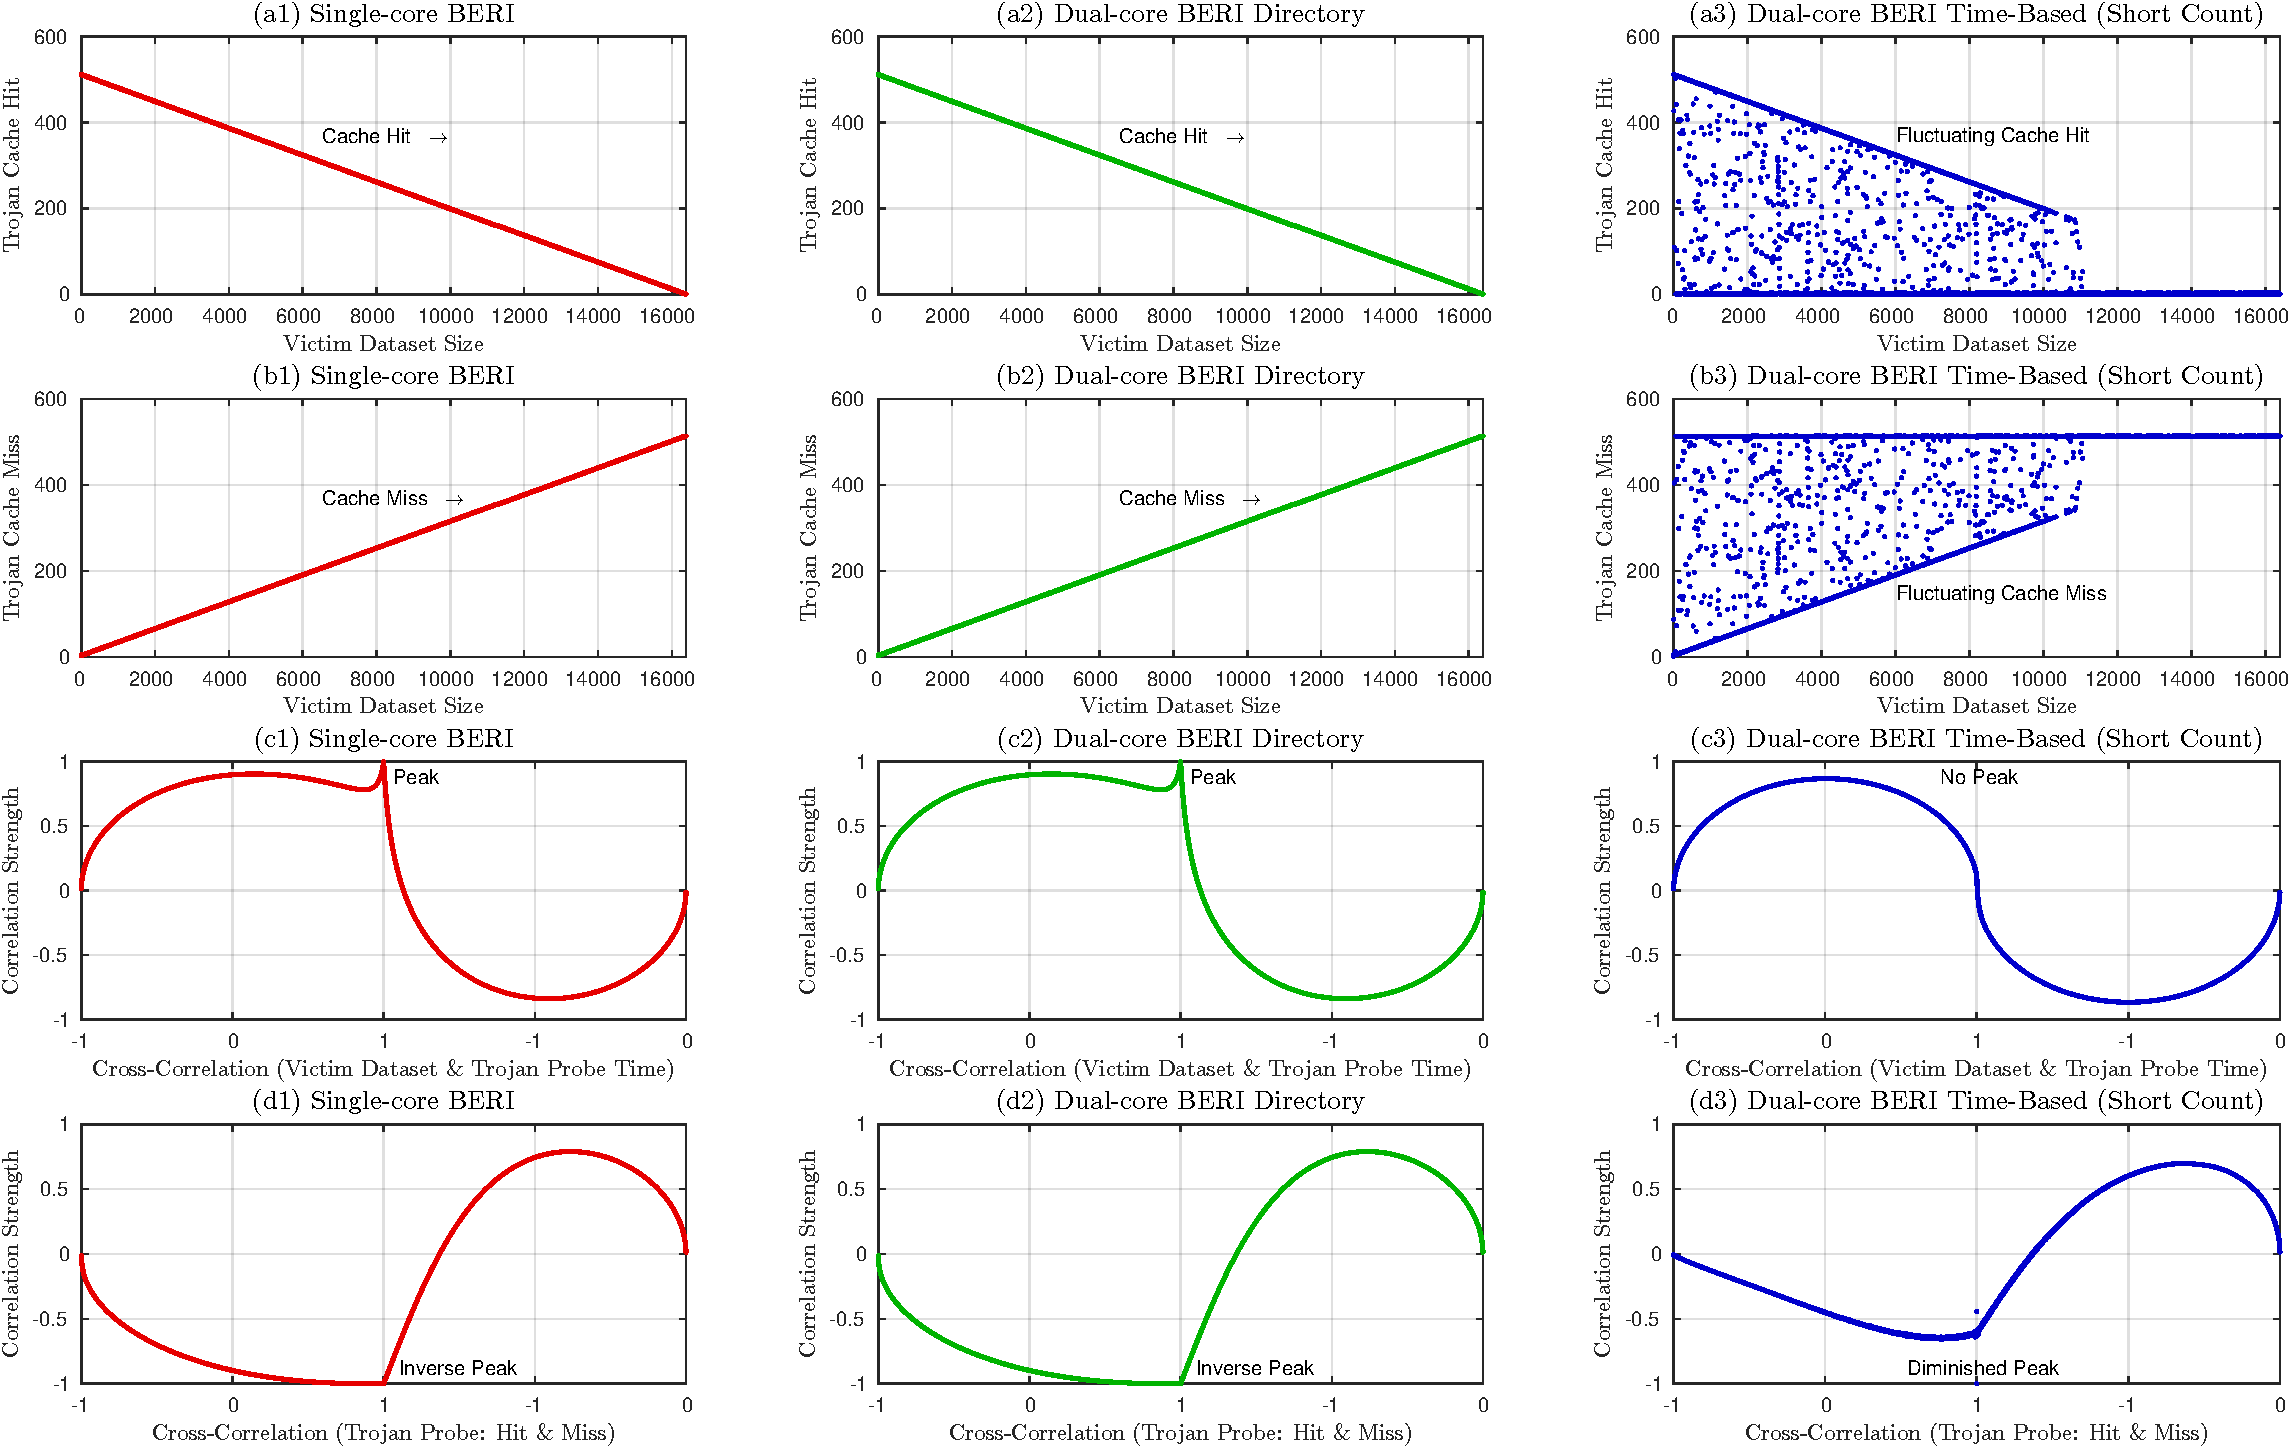
\includegraphics[width=\textheight,height=0.95\textwidth,keepaspectratio,angle=90]{sca_baremetal_standard_2x}}
						\caption{Bare metal side-channel attack, chart (1b)} 
						\label{baremetal_core_pin_std_2x}
					\end{figure}
			


\clearpage
				\paragraph{Figure \ref{baremetal_core_pin_long_1} --}
						In this figure we look at the side-channel leakage of a time-based coherence scheme using a long counter offset (100,000 cycles). Results for the directory scheme and the time-based model using a short counter offset (10,000 cycles) have already been discussed in Figures \ref{baremetal_core_pin_std_1} and \ref{baremetal_core_pin_std_2x}. They are used as a reference to highlight any additional side-channel leakage that may be produced by a less-aggressive self-invalidation scheme.
					\begin{description}
					\item [a(1,2,3)] 
						All models show a similar Victim execution time for a given dataset size.
					\item [b(1,2,3)]
						Charts a(1,2,3) are enhanced to highlight any fluctuations in the Victims execution time. The long counter offset time-based model  shows fewer time-counter overflows, as a result, only $\sim$1\% of all Victims code iterations show a slower execution time. Compared with the short counter model, the overall performance penalty caused by self-invalidates is significantly reduced. These results match the Splash-2 benchmark observations.
					\item [c(1,2,3)]
						Data shown in c(1) and c(2) has been previously discussed. The long counter scheme (shown in c(3)) preserves cached data for a longer time duration; thus, showing more side-channel leakage. The ideal leakage plot shows the expected outcome for a system without SCA protection, such as the directory model. The time-based model still offers some side-channel masking, but the leakage shown is sufficient for extracting useful information. Any Victim application with an execution time of 100,000 cycles or less will be compromised. 
						
						This example clearly shows that selecting a time-count offset is critical for SCA mitigation. I have already mentioned that inserting a SYNC instruction just after the Victims execution will be sufficient to mask side-channel leakage, this property holds for all offset values. If a SYNC instruction had been adequately used in this test, we would observe consistent data cache misses during the Trojan Probe phase.
					\item [d(1,2,3)] 
						Since the granularity of cache access timing is restricted to 32 bytes, we continue seeing the stepped pattern for the directory case. Note that the scale used to display charts d(1)--d(3) is identical, and the time-based short counter offset scheme does not show any samples in this range due aggressive cache self-invalidations. The pattern shown by the long count version is much closer to that shown by the directory model, but the time-based model still experiences a regular pattern of high latency. The noise is sufficiently low, allowing the attacker to extract useful information.
					\end{description}
				
				\paragraph{Figure \ref{baremetal_core_pin_long_2x} --}
					In this figure we look at the cache hit and miss count, as well as the correlation between data captured by the Trojan and known Victim behaviour.
					\begin{description}
					\item [a(1,2,3)] 
						Comparing the two time-based models we see that the long count version provides cleaner cache hit samples. While this data is not identical to the directory behaviour, we can observe a matching pattern. Unlike the short counter version, we do not observe a sharp drop-off in hits. The long count version experiences roll-overs 10 times less frequently.
						The Victims execution time never exceeds 250,000 cycles and the long timer offset model requires 1,600,000 (16$\times$100,000 cycles) cycles for a time-counter roll-over. 
						The counter roll-over is one of the major performance drawbacks of the time-based coherence model.
					\item [b(1,2,3)] 
						The observed miss counts are again inversely proportional to the corresponding hit counts and follow the expected behaviour. 
					\item [c(1,2,3)] 
						The previous set of results illustrated in Figures \ref{baremetal_core_pin_std_1} and \ref{baremetal_core_pin_std_2x}
						have established that the short counter time-based model does not demonstrate any correlation between the Trojan Probe data and the Victim behaviour. While the long counter model shows some correlation. However, when observing the full range of Victims data, a higher overall execution time will allow the time-based long counter to provide more side-channel masking.
					\item [d(1,2,3)]
						The correlation shown between the hit and miss count is significantly improved in the time-based long counter model. The purpose of this correlation is to identify any patterns in memory behaviour, this data is not normally available to the attacker. It also provides a good metric for comparing different versions of the SCA tests and time-based models.
					\end{description}
% Figure batch 2
					\begin{figure}[!h]
					\centering 
						\makebox{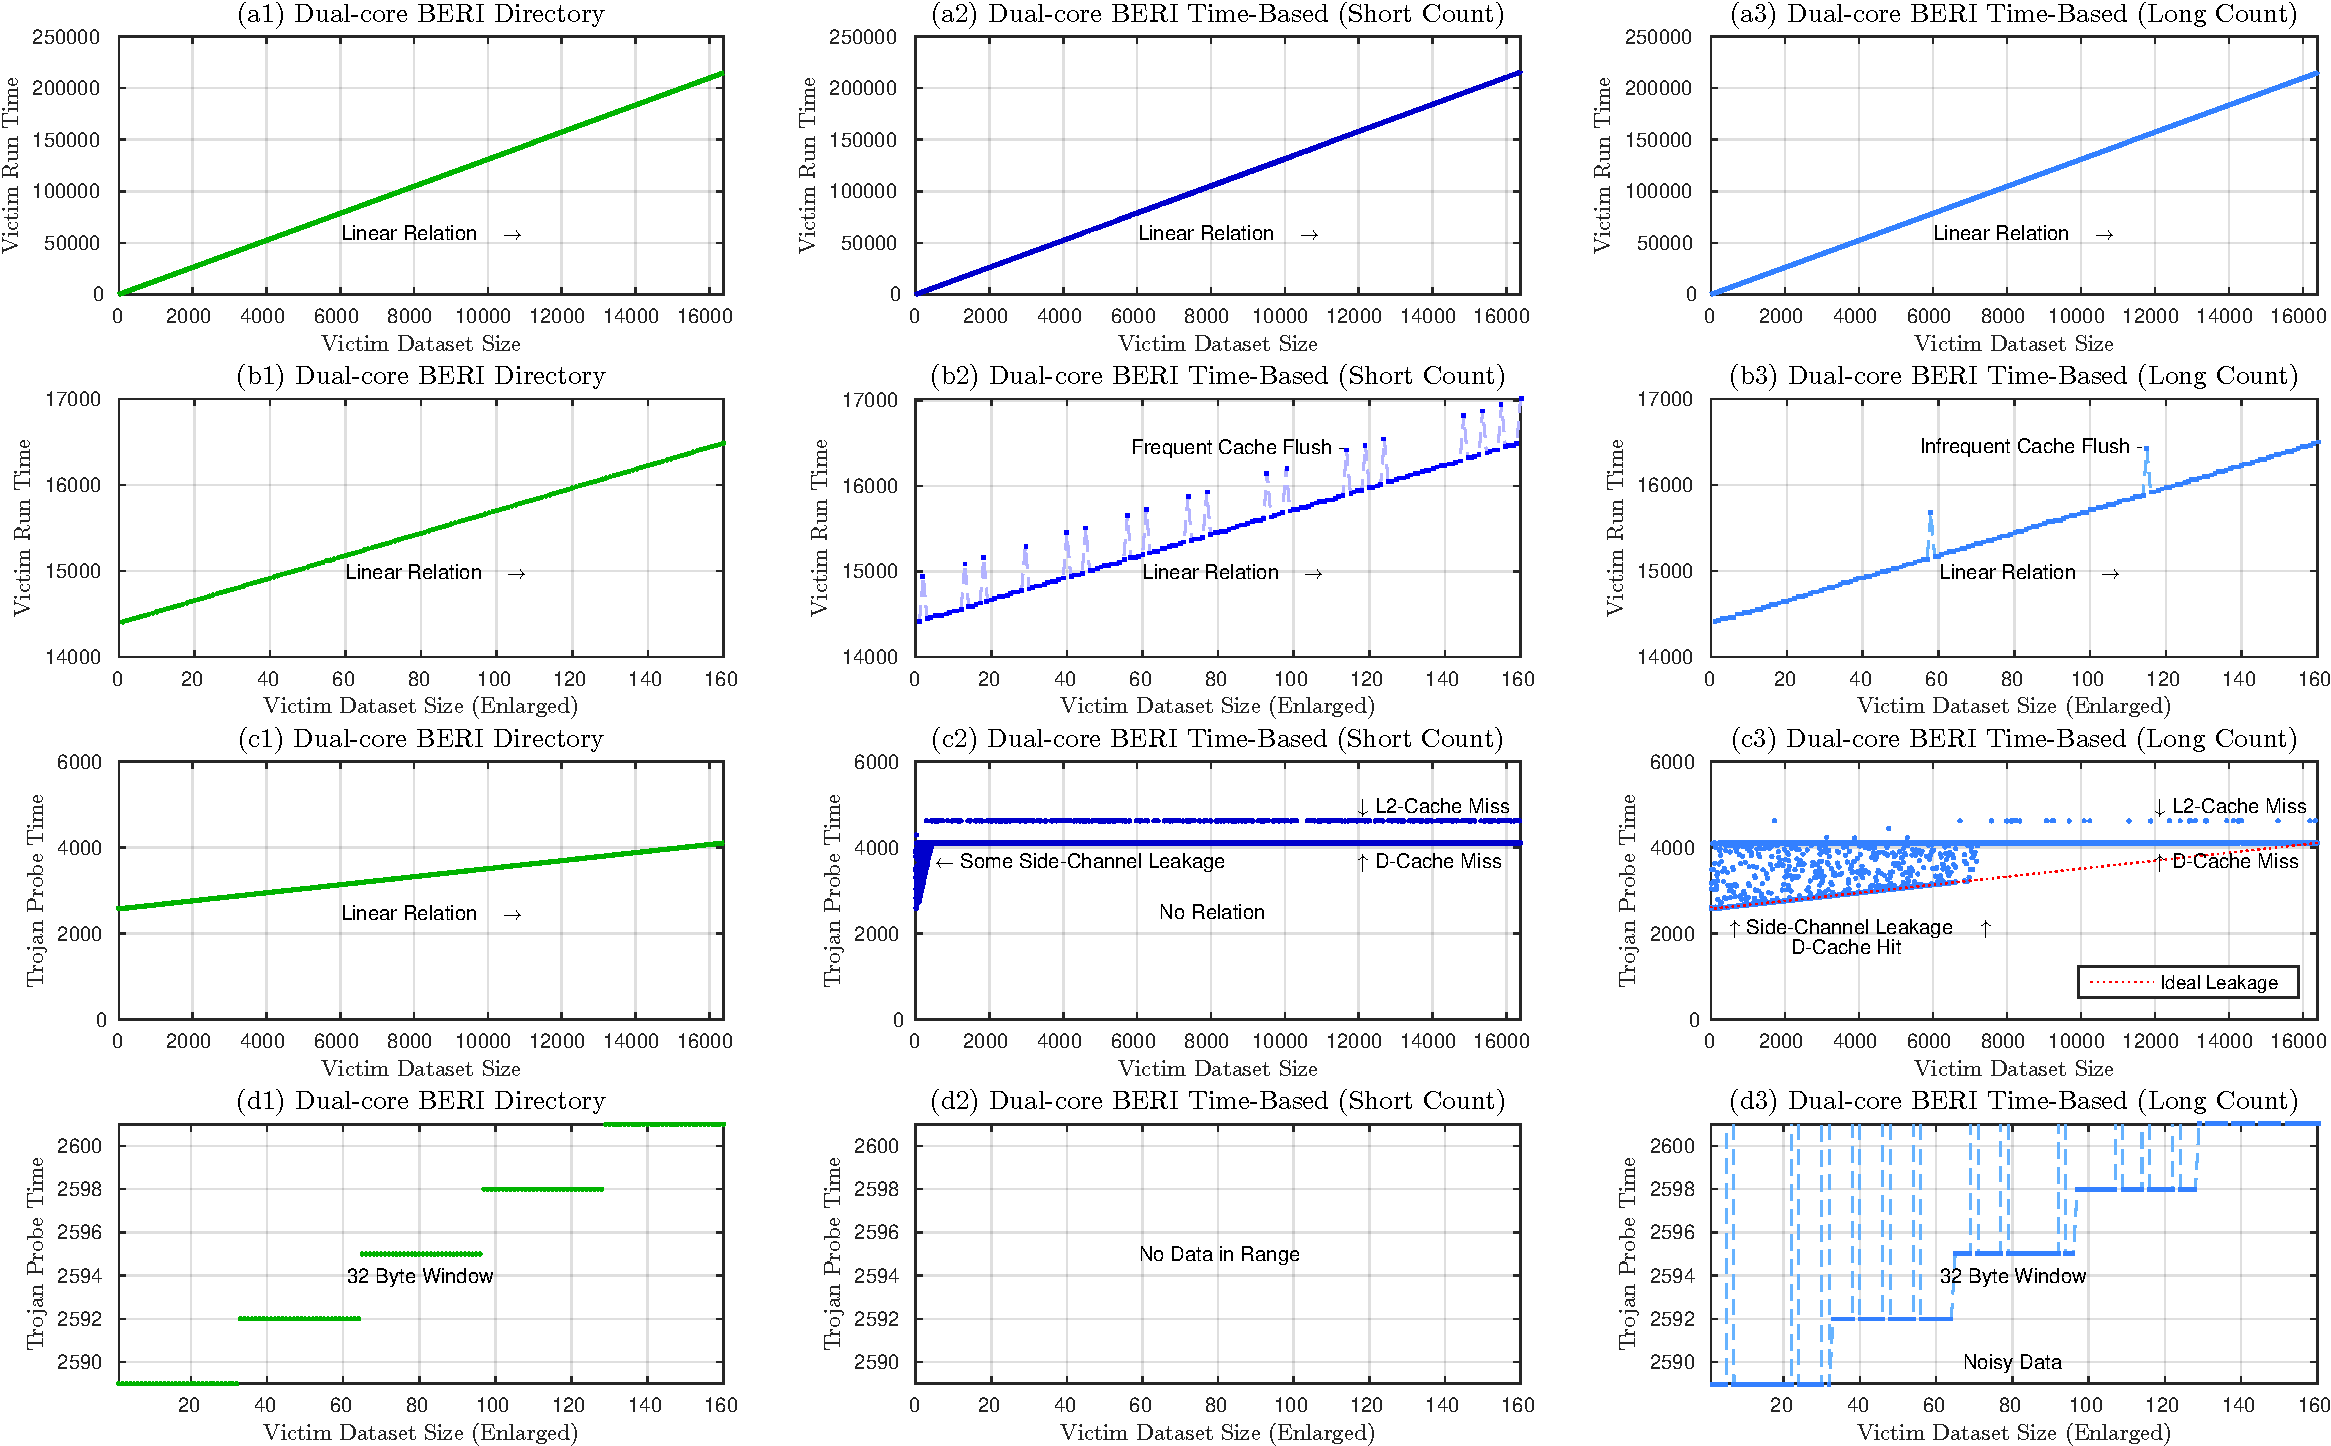
\includegraphics[width=\textheight,height=0.95\textwidth,keepaspectratio,angle=90]{sca_baremetal_long_1}}
						\caption{Bare metal side-channel attack, chart (2a)} 
						\label{baremetal_core_pin_long_1}
					\end{figure}
					
					\begin{figure}[!h]
					\centering 
						\makebox{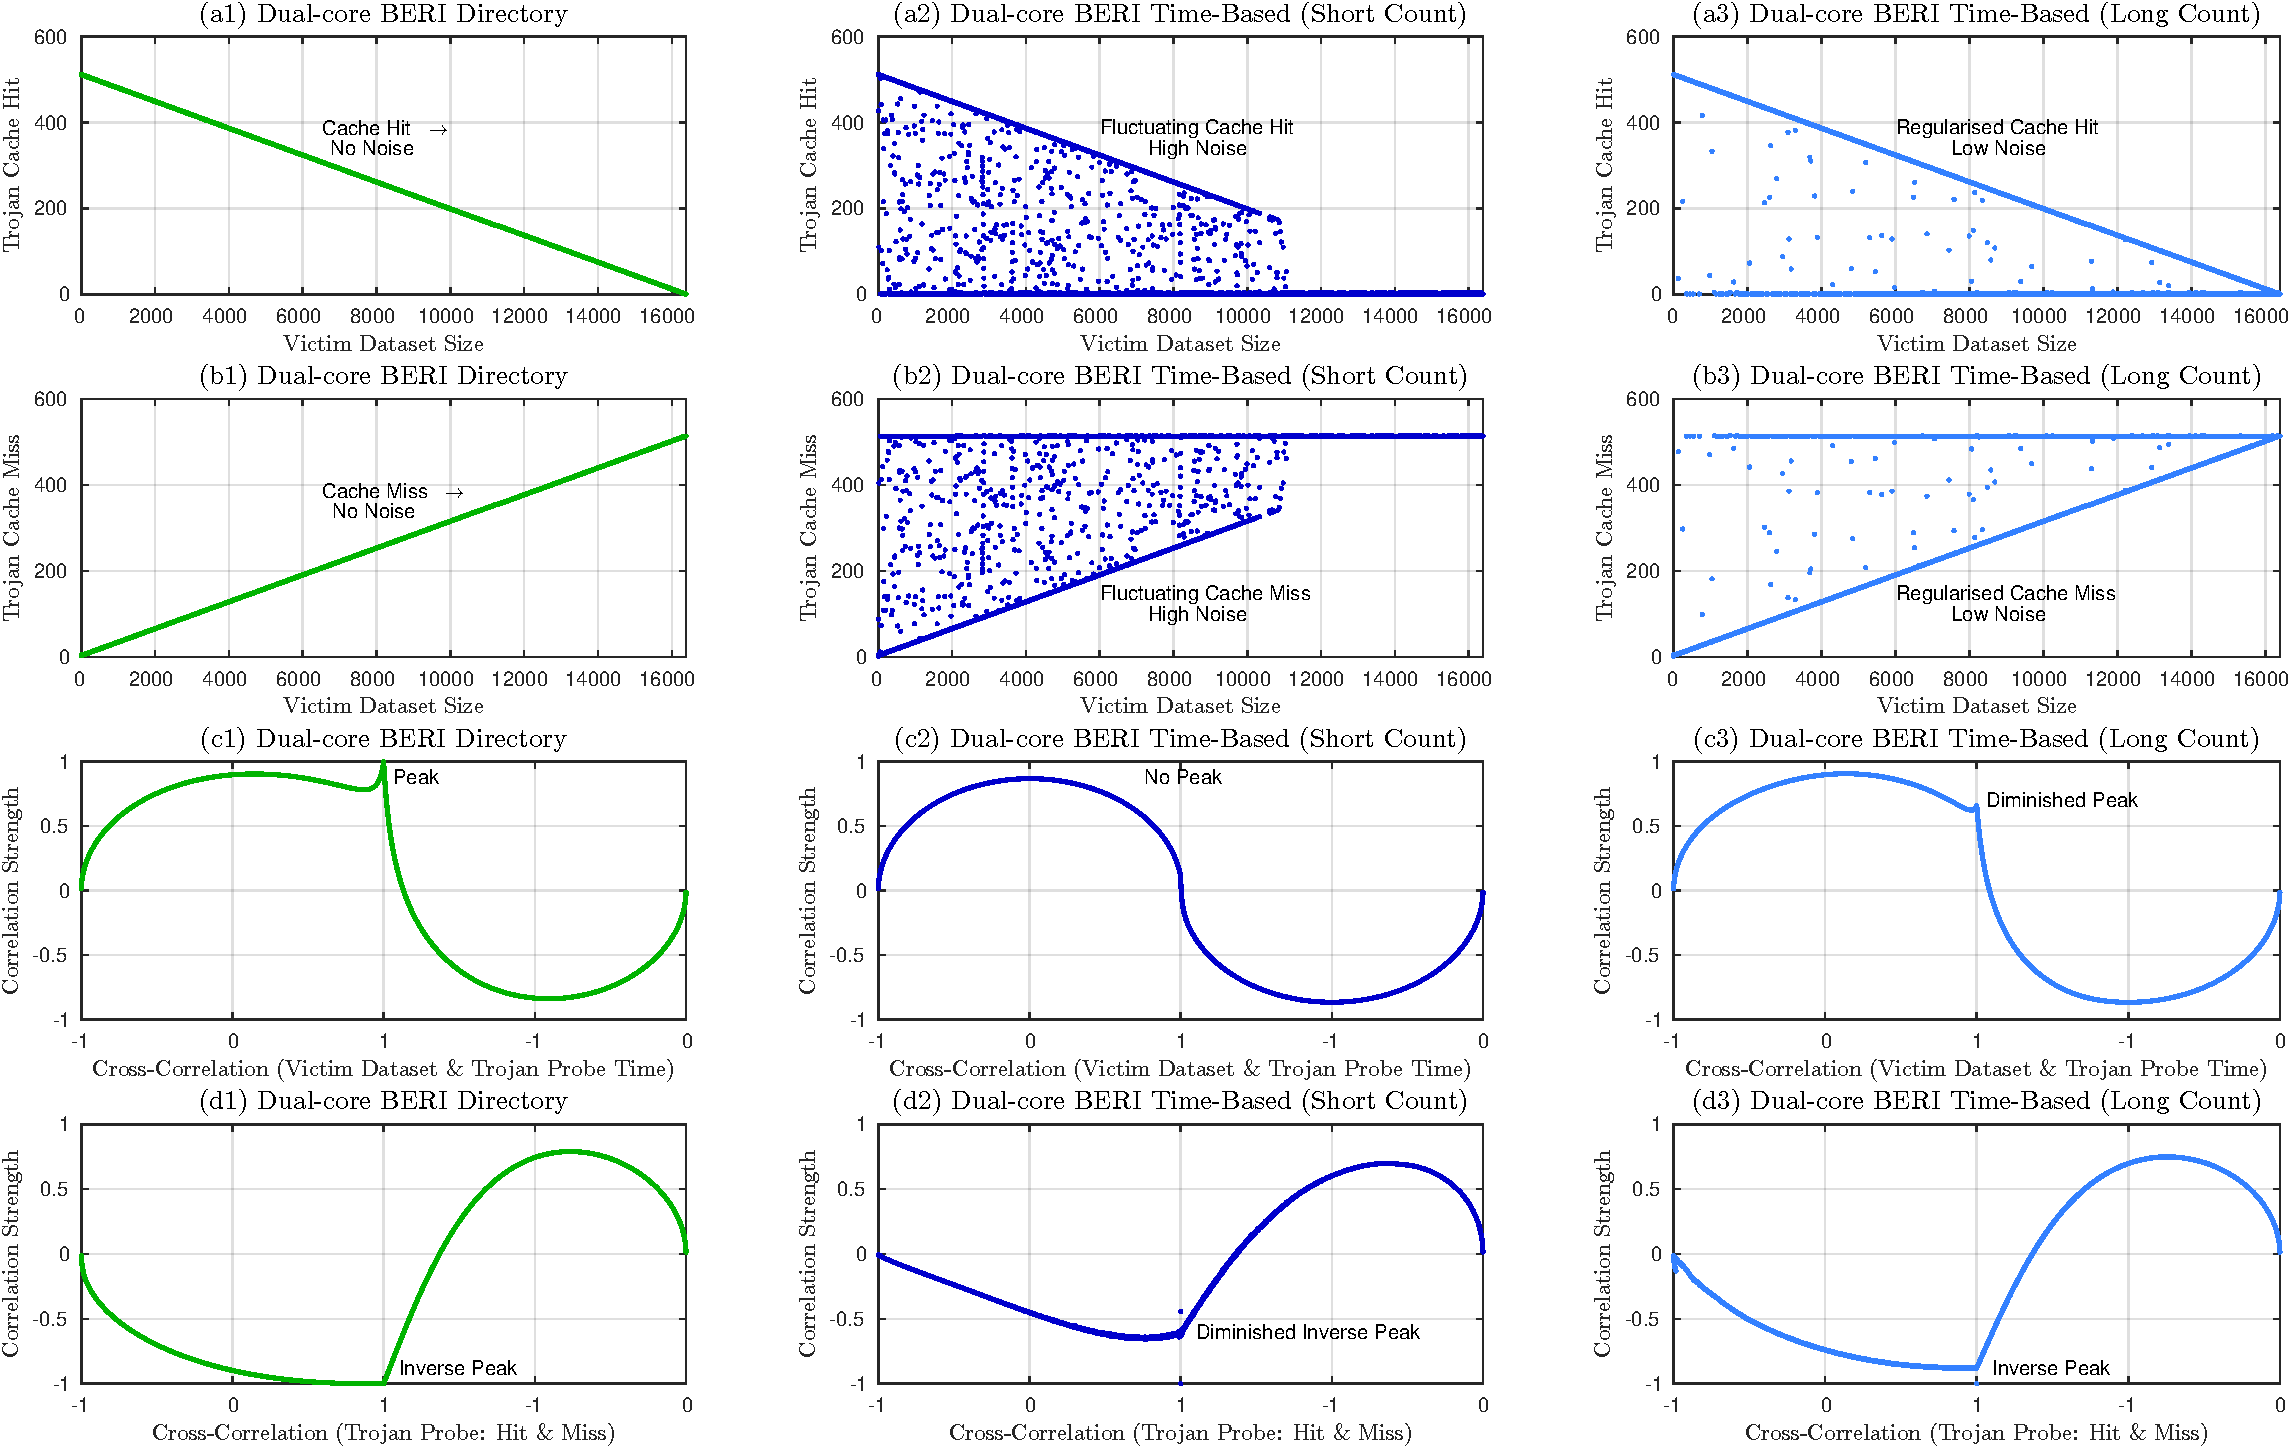
\includegraphics[width=\textheight,height=0.95\textwidth,keepaspectratio,angle=90]{sca_baremetal_long_2x}}
						\caption{Bare metal side-channel attack, chart (2b)} 
						\label{baremetal_core_pin_long_2x}
					\end{figure}


\clearpage
				\paragraph{Figure \ref{baremetal_core_pin_reverse} --}
					In the default SCA test, the Trojan Probe reads back data in the same ascending address order as the Prime phase. An attacker aware of the time-based coherence scheme may trick the system into leaking more side-channel information by probing data in a descending order (reverse test). 
					
					Most recent Trojan data is more likely to hold a valid tag-time-stamp, so evictions caused by the Victim could still be detected. The directory model is not displayed in this set of tests as the order of Probe acquisition makes no difference. Note that in this figure, data gathered for each model is displayed in rows, rather than columns. 
					\begin{description}
					\item [a(1,2,3)] 
						The default test running on the short count version shows minimal or no side-channel leakage. 
					\item [b(1,2,3)] 
						When the reverse test is executed on the short counter version, we observe a marginal increase in side-channel leakage. The timing data is very noisy, but cache hits and misses show a much clearer pattern than a(2) and a(3). 
					\item [c(1,2,3)] 
						The default test running on the long count version shows moderate side-channel leakage, sufficient to detect data usage by small Victim applications.
					\item [d(1,2,3)] 
						This test case shows by far the most side-channel leakage. The data is noisy but many samples fall under the ideal leakage curve. This test clearly shows that improving the attack technique could yield better Trojan results. 
						
						If the attack were to be conducted on a single memory line, sufficient sampling would result in a precise SCA. As mentioned before, the leakage can be eliminated by appropriately inserting a SYNC instruction or using a smaller counter offset. 
					\end{description}
% Figure batch 3
					\begin{figure}[!h]
					\centering 
						\makebox{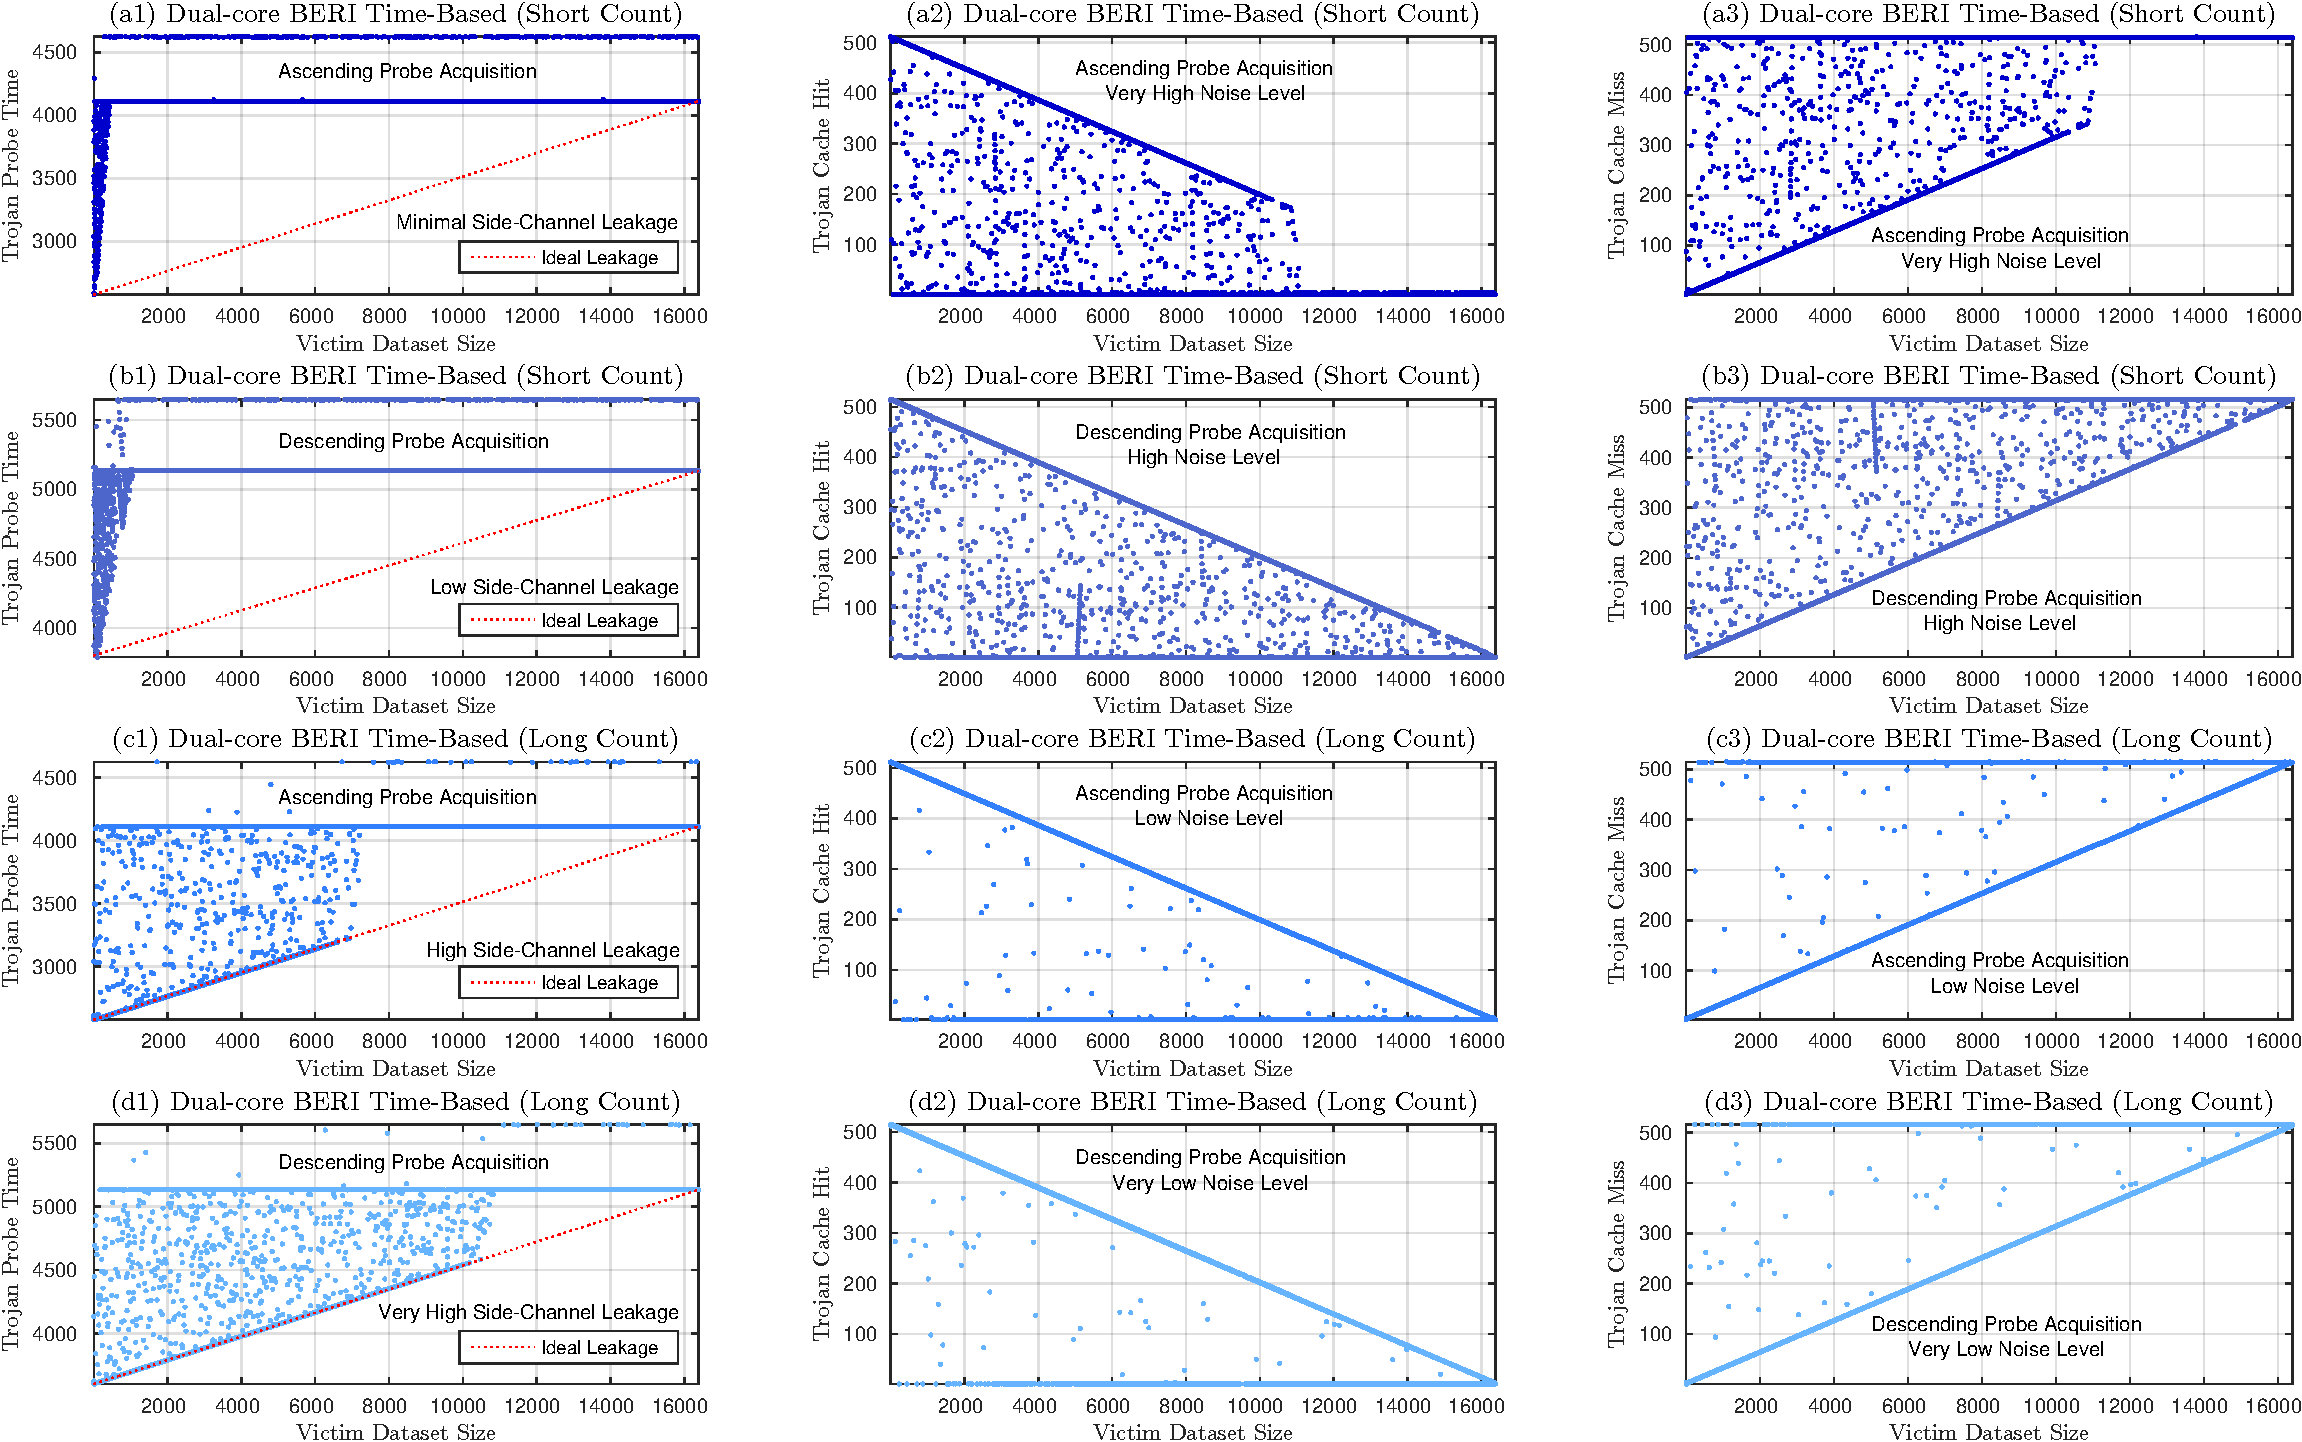
\includegraphics[width=\textheight,height=0.95\textwidth,keepaspectratio,angle=90]{sca_baremetal_reverse_1}}
						\caption{Bare metal side-channel attack, chart (3)} 
						\label{baremetal_core_pin_reverse}
					\end{figure}

\clearpage
		\subsection{Distributed Tests}
			In this test, the Trojan and Victim code segments are executed on separate cores, a highly likely scenario under OS support. The Trojan must now rely on any false sharing between its data and the Victims data in the L2 cache. The shared cache is much larger than the L1 data caches, so the likelihood of two program addresses mapping to the same cache line is lower.

			In the distributed test, Trojan code is executed on core 0 and the Victim code on core 1. Bare metal testing allows the master control program to delegate code-core allocation by reading the core ID's. During the Trojan Prime phase on core 0, core 1 is held in a wait loop. Once the Trojan completes, it signals core 1 through shared memory to begin Victim code execution. Once the Victim code completes, core 0 is signalled and the Trojan Probe phase is launched. For obvious reasons the split-core test cannot be evaluated on a single-core system.

			In order to launch the Trojan and Victim operations at the appropriate time, this test uses shared memory variables and SYNC instructions. From the description of time-based coherence so far, we have seen that stale data propagation may take a long time, to ensure quick and guaranteed updates, SYNC instructions are added after shared value updates.
			
			\paragraph{Expected Behaviour}
				The test datasets are designed to fit within the L1 data caches, so any misses will result in L2 lookups. The two cores have private L1 data caches, there will be no direct interaction between the Trojan and Victim. Memory aliasing may occur in the L2 cache which can influence the behaviour of both applications. 
				
				Time-based coherence does not provide shared memory SCA protection as it has no influence over it. In the absence of any direct memory interaction between the two codes, we do not expect to see any variation in Trojan Probe data.

			\paragraph{Observed Behaviour - Directory}
				Results match the expected behaviour, the Trojan Probe phase was not able to extract any useful information regarding the Victims dataset size. Table \ref{split_core_results} shows the obtained results. Notably the Trojan timing, miss, and hit results are constant, which is different to the time-based results.
				
				The same attack can be conducted on a larger scale, such as an L2 size Trojan Probe. Any memory aliasing between the two applications will leak exploitable side-channel information. Shared cache attacks are tested and evaluated further in this chapter.

			\paragraph{Observed Behaviour - Time-Based}
				As with the directory case, we do not observe any Trojan Probe timing fluctuations, only self-invalidation noise is present. The Trojan does encounter a higher miss rate due to self-invalidations, but the values are consistent throughout. The evaluated scheme is using a short counter offset, which has proven to provide better side-channel masking. However, this model adds performance penalties to the Victim execution, $\sim$8\%. 
				Note that the Victims execution time indirectly affects the Trojan Probe results. The wait time increases the likelihood of Trojan data self-invalidation.
				
				Two versions of the code were tested; SYNC based synchronisation and LL/SC based synchronisation. SYNC causes an immediate invalidation of all Trojan data, regardless of the Victims execution time, the Trojan always experiences maximum L1 data cache misses. The LL/SC case does not affect the time-based coherence mechanism. The Trojan may see data cache hits if the Victim execution time is low, the mean Trojan Probe cycles are slightly lower when using this synchronisation mechanism. The results show very little variation, summarised in Table \ref{split_core_results}. 
			
			\begin{table}[!h]	
			\begin{center}					
			\begin{tabular}{|l||c||c|c|}
				\hline
				\multicolumn{1}{|c||}{Parameter} & Directory & \multicolumn{2}{|c|}{Time-Based} \\
				\cline{3-4}
				& & SYNC & LL/SC \\
				\hline
				\hline
				Victim Cycles (Mean) & $\sim$77,000 & $\sim$83,000 & $\sim$83,000 \\
				Trojan Cycles & 2080 & $\sim$3650 & $\sim$3600 \\
				Probe Miss & 7 & 513 & $\sim$513 \\
				Probe Hit & 506 & 0 & $\sim$0 \\
				\hline
			\end{tabular}
			\caption{Bare metal distributed side-channel attack}
			\label{split_core_results}
			\end{center} 
			\end{table}


\clearpage
	\section{SCA Testing Including an OS}
		\label{os_prime_probe_attack}

		Performing a side-channel attack in a controlled simulation environment has precisely shown the advantages and pitfalls of using time-based coherence as a mitigation technique. Testing on an OS presents different challenges: scheduling effects, interrupts, kernel processes, and other user processes. In this set of tests the Trojan and Victim applications are the only user processes operating on the system. The bare metal code used previously was modified and recompiled to run under FreeBSD on BERI. In order to control the allocation of Victim and Trojan codes to a given core, I use the core affinity functions available for FreeBSD \cite{cpuaffinity_0,cpuaffinity_1}. 
		
		The Victim and Trojan are spawned through the same executable, however, the two applications are forked, enabling independent OS control and a different address mappings. The individual program behaviour is not modified, thus a successful attack should display results very similar to those shown in the bare metal versions. 
		
		Another significant difference in the OS tests is the timing of Trojan Probes, FreeBSD does not allow access to some hardware counters in userspace, but an OS clock function is accessible. The clock precision was sufficient to observe the expected behaviour. The hardware counter is available to use in a privileged mode but I opted out of this option since a potential attacker would not have this access.

		A total of 5 sets per test configuration were acquired, each set iteration captures 10,000 Trojan timing samples. Each timing sample is the total time taken for the Probe phase. Averaging this access time across all samples will reduce noise and provide a mean latency for a given set of test parameters. Sets are analysed individually and compared to observe any deviations. In order to improve the execution time, the bare metal test was simplified. The granularity of Victim data size increments was reduced to a total of 9 settings, starting from no data usage as a control, to full data cache capacity. 
		
		The test was also extended to Probe the L2 cache. In this version the Trojans dataset is sized to match the L2 cache. The Victim dataset is limited to the size of the L1 data cache. The Trojan Probe will incur L1 data cache misses, as the dataset is larger than L1 data cache capacity. The Probe should be able to observe misses due to evictions in the L2 cache.

		In this set of tests I use the ascending address attack. It ensures that data cache hits are not observed and all memory accesses end-up in the L2 cache, thus observing L2 cache hits and misses. 

\clearpage
		\paragraph{Figure \ref{freebsd_sca_corepin_1} --}
			This figure shows an SCA attack on the L1 data cache. The Trojan dataset size is equal to the L1 cache capacity.
			\begin{description}
			\item [(a1,b1,c1,d1)] 
				This chart group shows the median latency for the Probe phase for each Victim dataset size. Data in each chart is normalised using the minimum sample value. 
				
				The control measurement where the Victim size is zero, shows the baseline measurement. Interestingly, all the models show a consistently low value for this measurement. This is likely due to minimal interference from any other processes and other cores. 
				
				The single-core and directory versions both show a low standard deviation in values and provide the most confidence in the results. The single-core version shows a slight data deviation from the base sample to the first Victim size of 2K. This model has only one core to execute all processes, so a minimal gap between measurements will show lower interference from the rest of the system and an overall execution time. The trend line for both single-core and directory is representative of the expected behaviour and confirms the possibility of a SCA.
				
				Time-based short count version shows a high level of error and a very high miss rate for all samples other than the control. The control latency is understandable as there is no Victim execution and the Trojan Probe can begin almost immediately after the Prime phase.
				Time-counter roll-overs and L2 cache misses are also less likely in this case. 
				
				The long count model shows similar behaviour but with a much lower error rate. It still shows a flat trend for all but control samples. Some side-channel leakage is expected, as seen in the bare metal tests. 
				\textcolor{red}{The reason we may not be seeing as much leakage as the bare metal version is due to all the external factors such as the OS scheduler, interrupts and other processes.}
				Self-invalidation is very sensitive to timing so any delays inserted between the Prime and Probe phases can have profound effects on the timing results. 
			\item [(a2,b2,c2,d2)] 
				Each chart shows a normalised correlation between the acquired Probe timings and the increasing Victim memory footprint. The curves shown in charts (a1,b1,c1,d1) are compared against the Victim footprint (0K--16K \textcolor{red}{units}). 
				The single-core and directory designs, both show a strong correlation, indicating that the Trojan behaviour consistently follows the Victim behaviour. Knowing the timing curve shown in (a1,b1), we should be able to identify the memory usage of a Victim for any range that falls within the data cache.
			\end{description}

\clearpage
			\begin{figure}[!h]
			\centering 
				\makebox{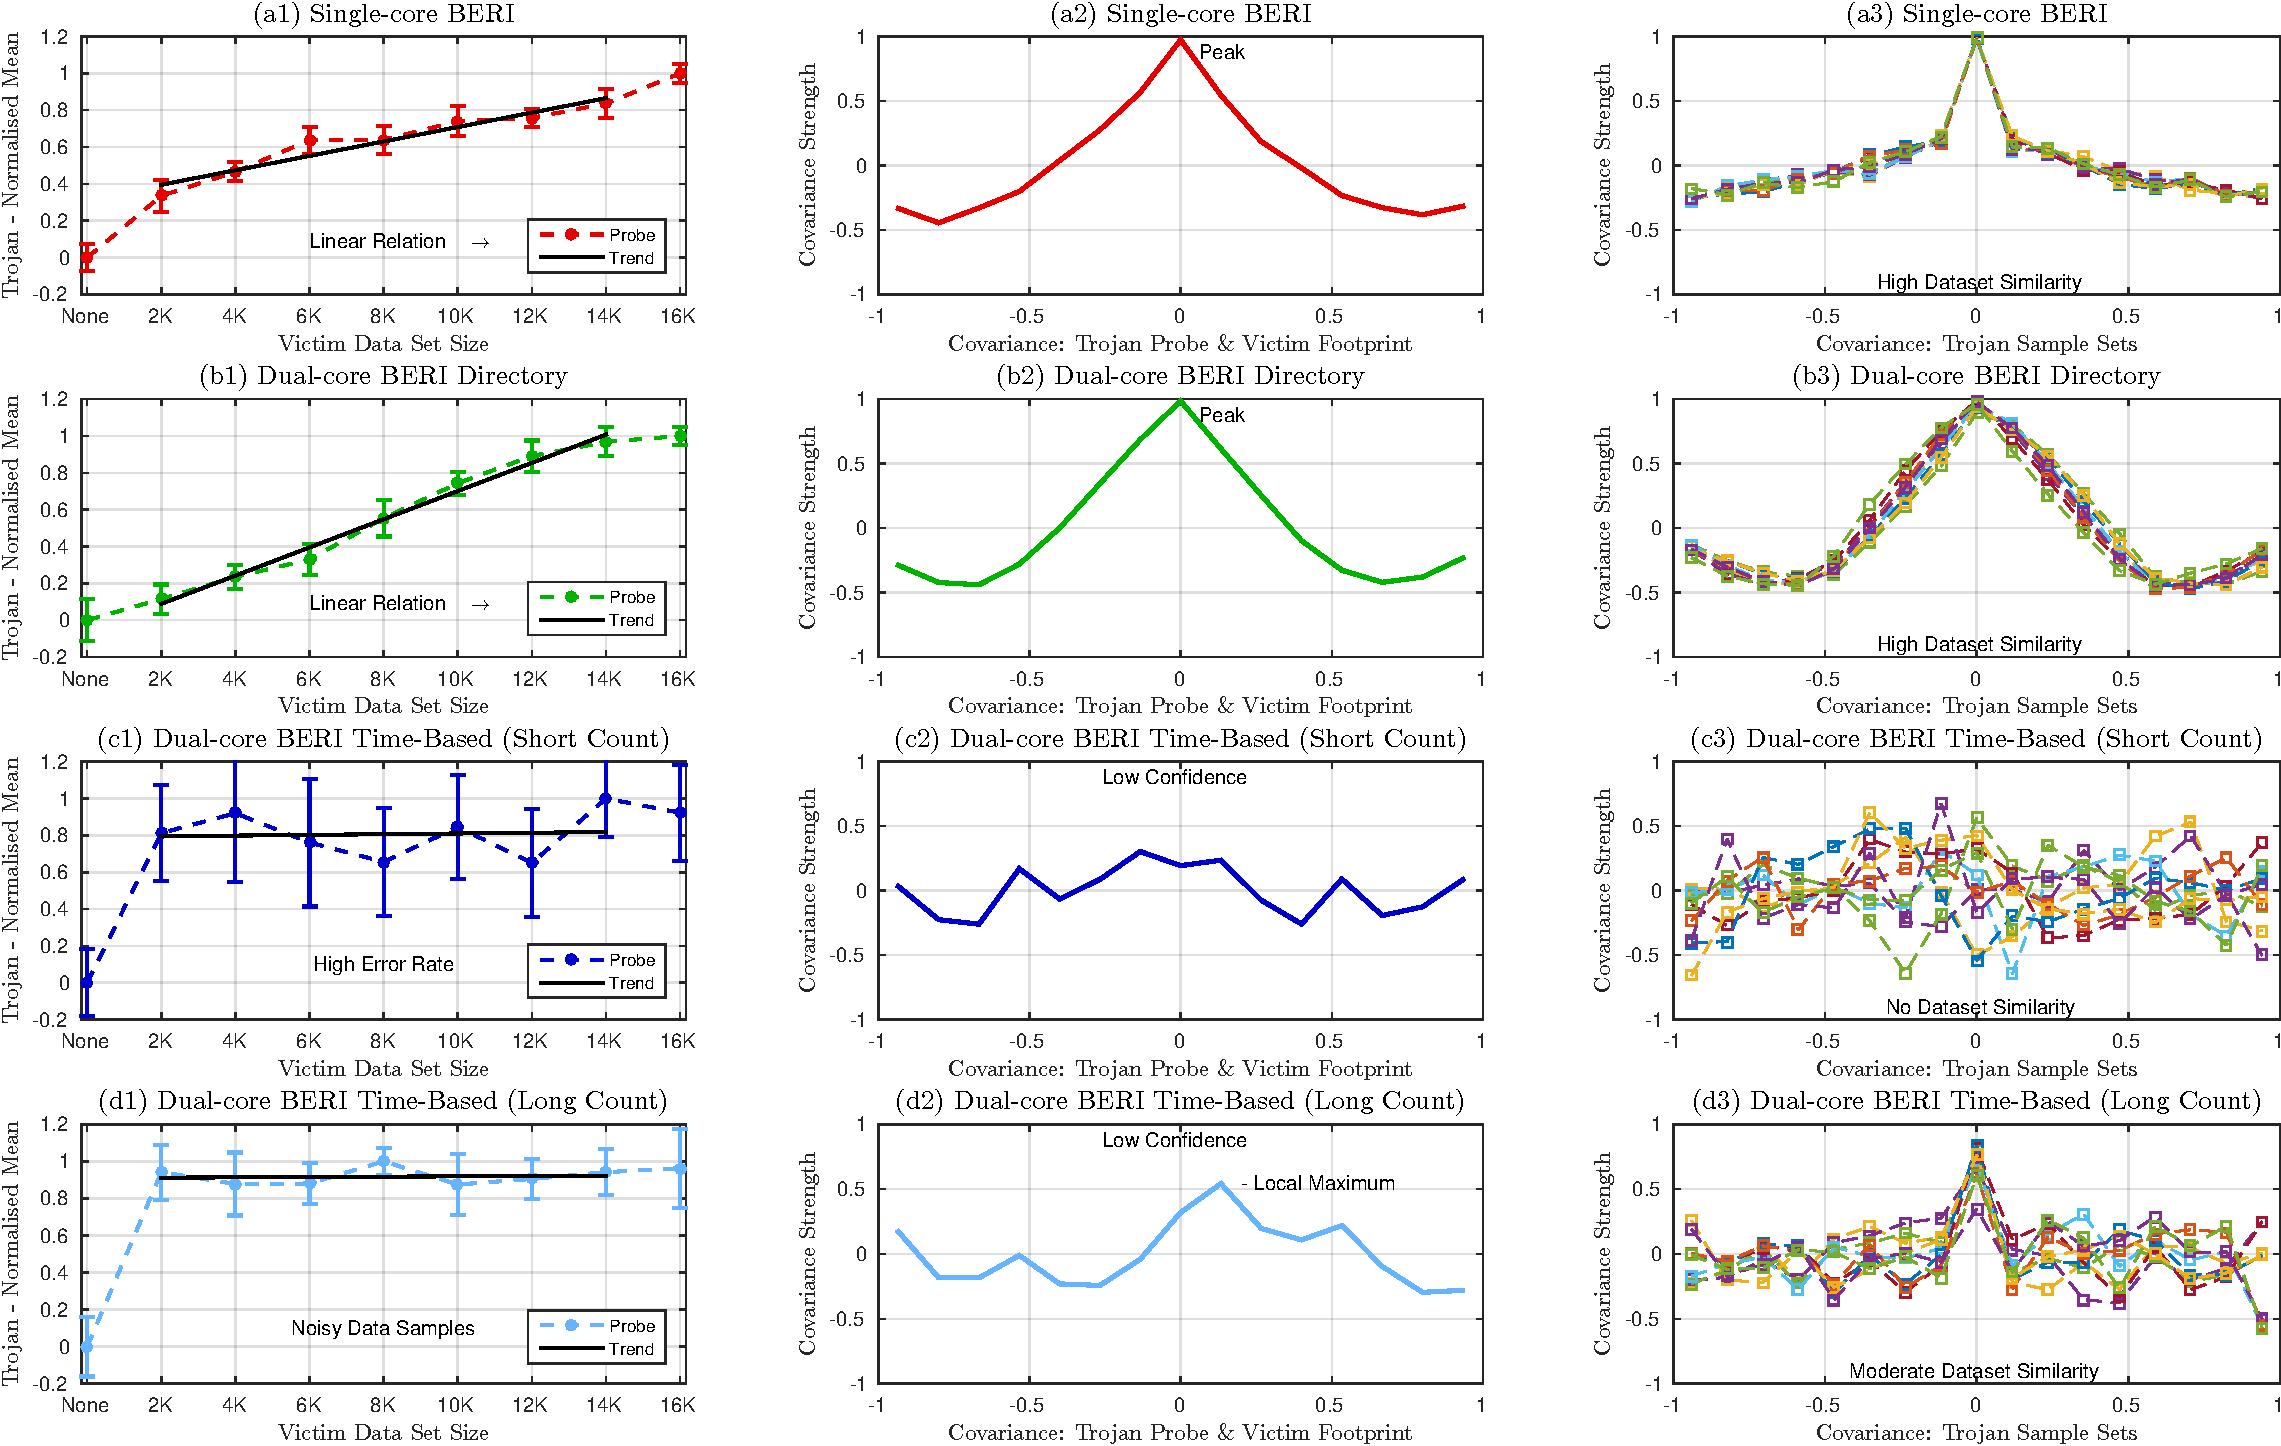
\includegraphics[width=\textheight,height=0.95\textwidth,keepaspectratio,angle=90]{freebsd_sca_corepin_1}}
				\caption{FreeBSD side-channel attack (L1 data cache)} 
				\label{freebsd_sca_corepin_1}
			\end{figure}

			\begin{figure}[!h]
			\centering 
				\makebox{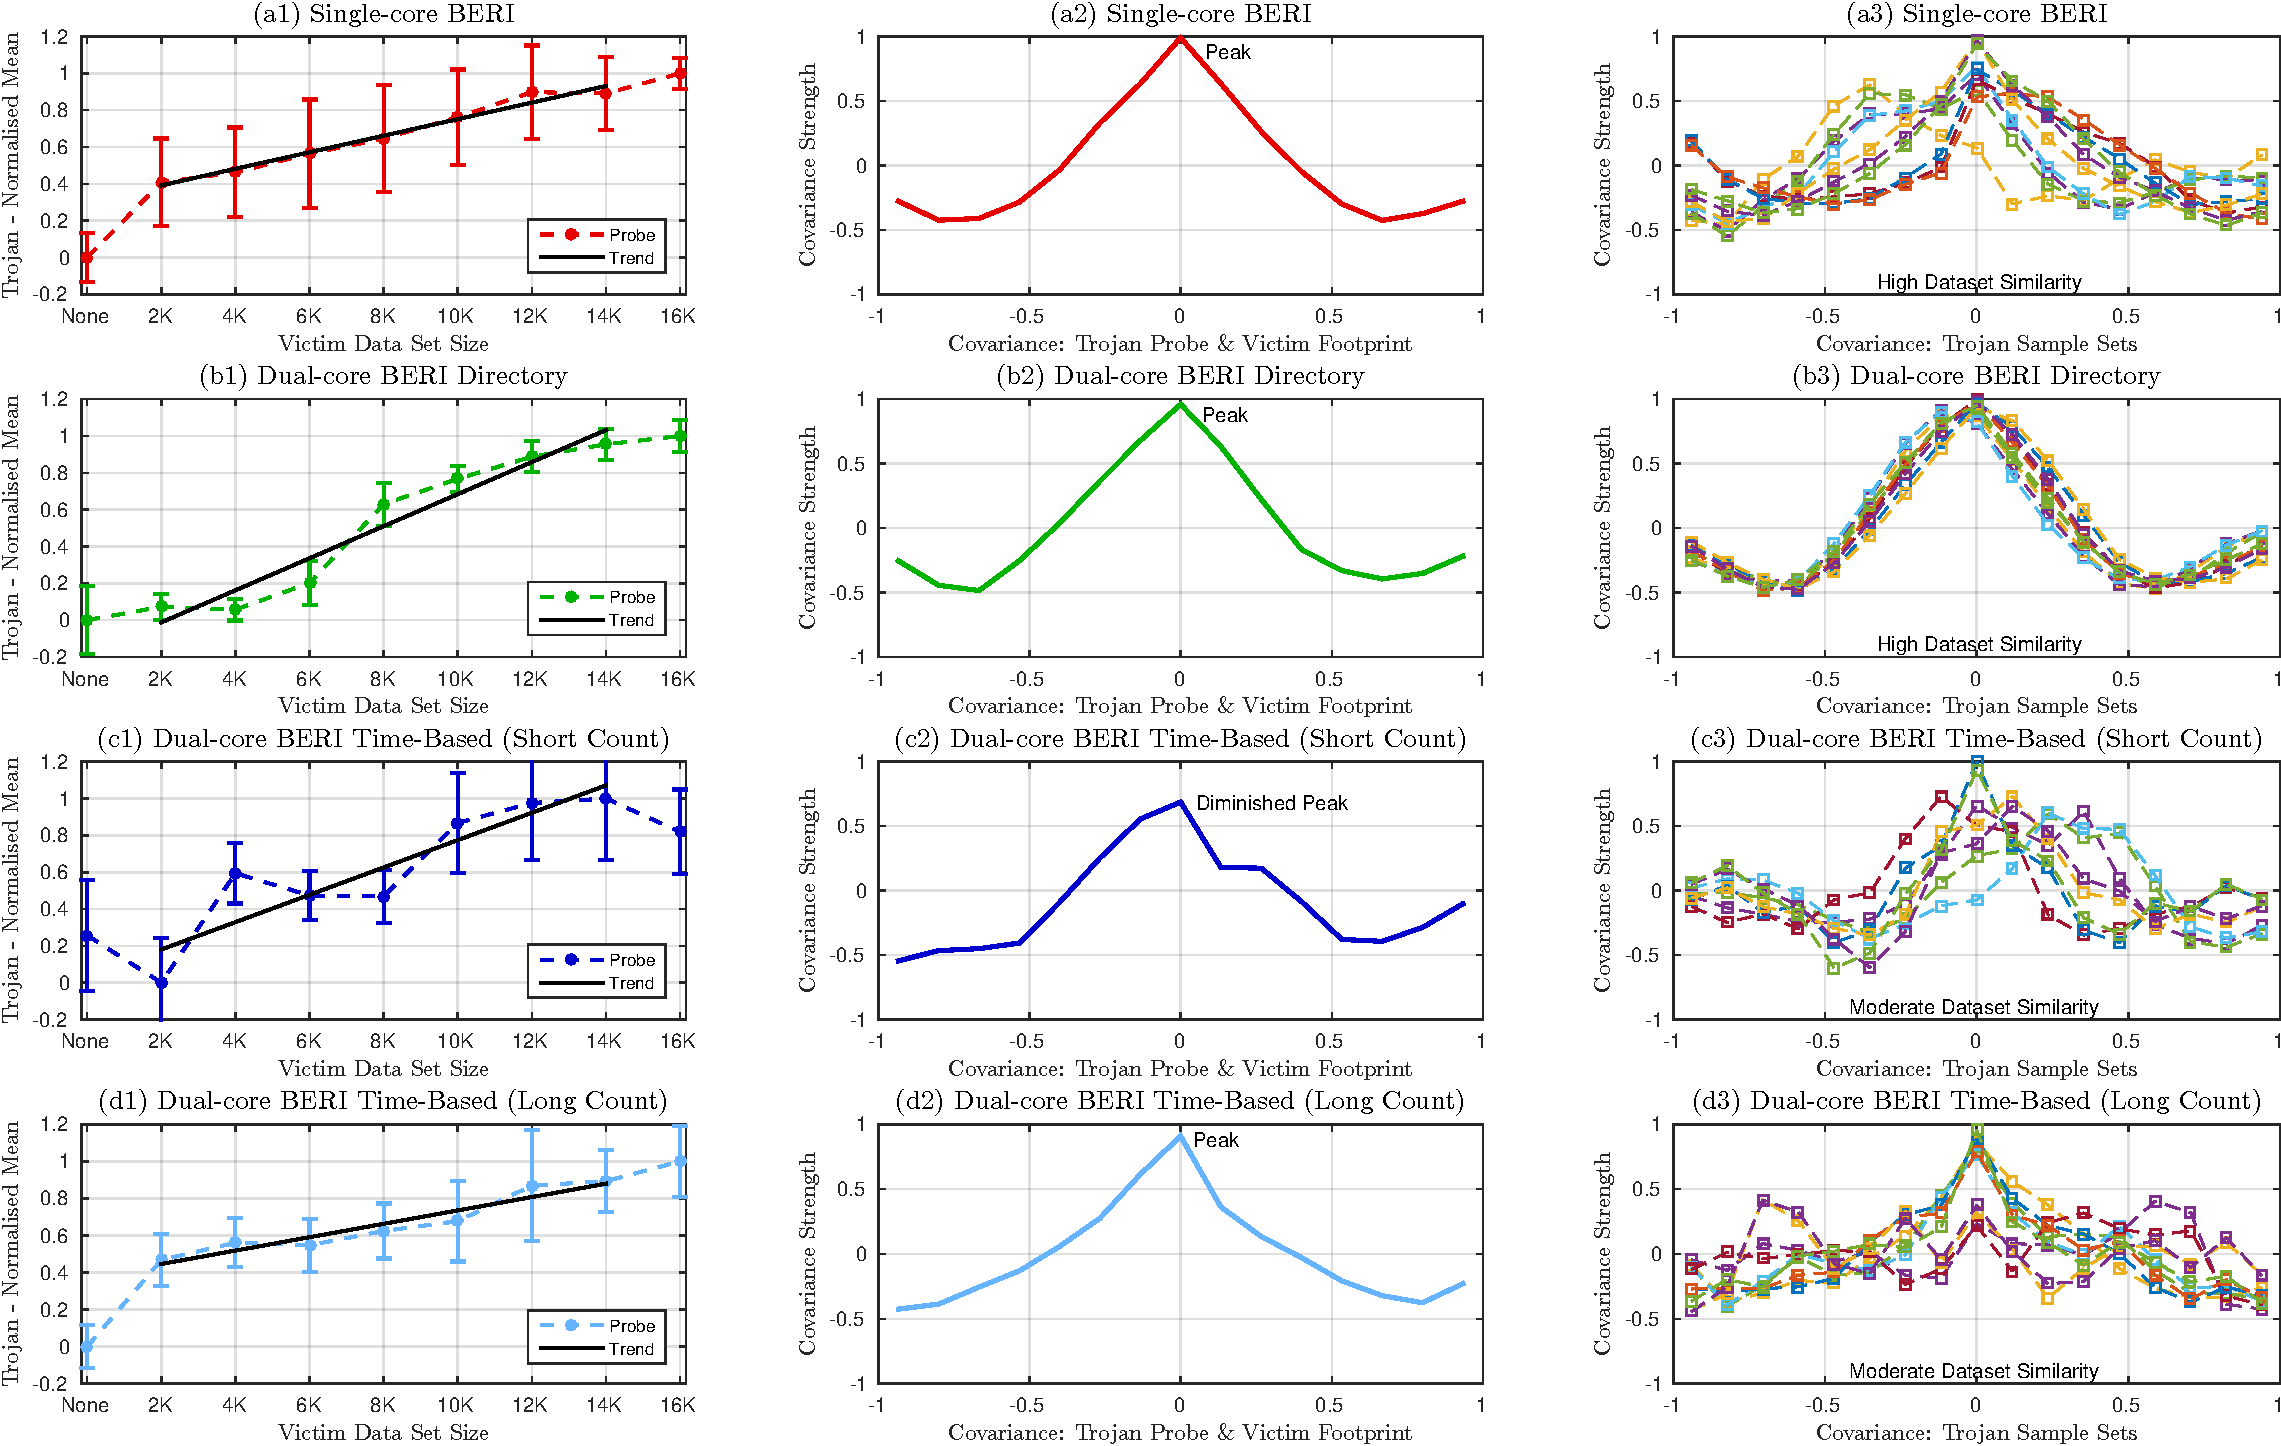
\includegraphics[width=\textheight,height=0.95\textwidth,keepaspectratio,angle=90]{freebsd_sca_corepin_2}}
				\caption{FreeBSD side-channel attack (L2 cache)} 
				\label{freebsd_sca_corepin_2}
			\end{figure}

\clearpage
			\begin{description}
			\item[\ \ \ \ \ ]
				Both time-based versions do not show a clear correlation. However, the long count version shows a minor correlation. Added Trojan sampling may be sufficient to profile this behaviour.
			\item [(a3,b3,c3,d3)] 
				In this chart we look at the similarity and reproducibility of acquired Trojan timing sets. A total of 5 sets were captured, yielding a total of 10 unique comparisons. The single-core and directory models show strong correlation between all datasets. Time-based coherence shows moderate correlation between datasets for the long count version. The short count version shows no correlation between the datasets.
			\end{description}
			
			
		\paragraph{Figure \ref{freebsd_sca_corepin_2} --}
			This figure shows an SCA attack on the L2 cache. The Trojan dataset size is equal to the L2 cache capacity.
			\begin{description}
			\item [(a1,b1,c1,d1)] 
				All charts show a common trend, Trojan time increases proportionally with an increase in the Victims dataset size. This acts as a confirmation that none of the models are protecting side-channel leakage in the shared L2 cache. Note that the observations show the mean timing information for 2048 memory accesses. The Trojan Prime phase bypasses the private cache and hits in the L2 cache. 
				
				Cache lines are not self-invalidated in the L2 so both the time-based models in (c1) and (d1) show leakage. The short count version is a little more erratic as the timing operation and general latency is likely affected by the self-invalidation mechanism. 
				
				SCAs on mechanisms such as AES require much finer timing granularity as well as the knowledge of precise latencies for each level of the cache. This test is demonstrating the amount of leakage by evaluating the average Trojan slowdown.
			\item [(a2,b2,c2,d2)] 
				The correlation charts show that each model demonstrates side-channel leakage. (c2) shows a diminished peak, however, the correlation is strong enough to profile the cache behaviour. A larger number of samples will likely present a much more accurate profile.
			\item [(a3,b3,c3,d3)] 
				The inter-set sample correlation shows that the directory provides the most reliable results out of all the models under test. Some noise is present in the single core case, likely due to other processes and interrupts. Both the time-based models are noisy, however a distinct pattern can be observed. 
			\end{description}



\clearpage
\section{Protection Level of Time-Based Coherence}
	The evaluation so far has demonstrated that time-based coherence injects some entropy into the timing data acquired by the Trojan. Several factors influence the effectiveness of this data randomisation: self-invalidation timing, critical application execution time, synchronisation instructions, the SCA target cache, number of Trojan samples, and the SCA technique.
	
	\begin{itemize}
		\item Self-Invalidation timing: The rate of data eviction in the L1 caches is directly proportional to the time-counter offset value. However, the Splash-2 benchmark results have shown that a lower time-out will cause a higher miss rate for any current application, resulting in a weaker performance. A longer time-out will improve performance but also retain the Trojan data. There is a tradeoff between application performance and side-channel leakage. Overall, time-based coherence provides more SCA mitigation than directory-based coherence, which provides none.
		%\item Application execution time: This factor ties in with self-invalidation timing, as a quicker/shorter application runtime will require a shorter self-invalidation time in order to ensure Trojan data eviction. Similarly a longer application execution time will allow using a longer TTL.
		\item Instructions: The SYNC instruction acts as a single cycle L1 data cache flush. A critical application can use this instruction before or after its execution, ensuring eviction of all L1 data. Similar techniques have been proposed and used on other systems (summarised by Osvik and Tromer \cite{Osvik06,Tromer10}), however, other systems may require explicit cache line invalidate instructions to achieve the same effect. The added instructions will cause pipeline stalls and degrade overall performance. 
		Most will argue that security overheads of the critical application are already large enough to ignore relatively small overheads caused by cache invalidate instructions, but this factor is still worth considering. One advantage of the SYNC mechanism is that the critical application requires no OS support for issuing the cache flush. Other systems may require system calls to request cache invalidation.
		\item Target cache: Time-based coherence SCA mitigation is effective in the L1 data caches. It provides no protection for the shared/last-level cache. Successful attacks on LLC's and other lower levels of memory have been demonstrated before \cite{Irazoqui15,Yarom14,Hund13,Brumley11}. Even if we can protect the LLC, attacks can be conducted on other levels of memory, such as DRAM, where other SCA techniques yield critical data. Time-based coherence can provide a level of SCA mitigation for virtual machines running on the same physical core.
		\item Trojan sampling: Time-based coherence follows a predictable self-invalidation pattern for a given cache line. A clever Trojan program may be able to carefully profile the entire cache behaviour. Repeated measurements will extract the self-invalidation timing parameters which the attacker can exploit by modifying the SCA technique. This issue can be circumvented by using software tunable dynamic self-invalidates or inserting SYNC instructions after the critical application. Even if the Trojan profiles the cache behaviour, there is little that it can do to prevent the effects of SYNC.
		\item SCA technique: In this chapter I have mostly discussed the Prime+Probe attack. It is a powerful technique when used correctly. A number of other techniques exist, these can be more or less effective against different mitigation techniques. Time-based coherence works well against Prime+Probe on L1 caches, but unlikely to defend against attacks on lower levels of memory.
	\end{itemize}
	
\section{Protecting the LLC}
\label{protecting_llc}
	The time-based coherence mechanism does not require any modifications to the LLC. We have established that the single cycle cache flush based on SYNC operations provides strong SCA protection in the private caches, a similar mechanism can be implemented in the shared cache. The LLC only needs the single cycle flush and does not require any automatic time-based self-invalidation. When the mechanism used in the private caches is integrated into the LLC, the cycle counter can be disabled. Without this counter the LLC will never perform an automatic time-based self-invalidate, thereby removing any performance drawbacks. 
		
	On SYNC instructions, the private caches can increment their local time-counters as well as propagate the instruction into the LLC. The LLC will then increment its own time-counter, thereby marking all cached data as invalid. This will guarantee side-channel masking. This scheme has some drawbacks, if the LLC is large, the resulting cache trashing will be expensive. Excessive use of SYNC instructions will cause frequent and undesirable trashing. These choices are design dependent and the need for side-channel mitigation may outweigh the drawbacks. Another drawback is that most shared caches use the write-back policy, increasing the challenge of incorporating self-invalidation, I discuss a solution to this issue in Section \ref{section_cache_properties}. Periodic flushing of dirty lines should simplify tracking lines and retain the advantages of write-back caches.

\section{Summary}
	As with many SCA mitigation techniques, time-based coherence increases the challenge of extracting useful timing information for the attacker. However, this technique is not fool proof and does not provide all aspects of SCA protection. If a system is build with this coherence model then it will possess some SCA protection out of the box, more than the standard systems. However, if any critical application is to be truly protected, other SCA mitigation techniques will be necessary. 
	
	Designers have already resorted to using dedicated hardware for both protecting and improving the performance of algorithms such as AES. Additionally, modern systems have sophisticated memory designs, allow out-of-order operations, and other optimisations, making SCAs even more challenging \cite{Tromer10,Mowery12}. Since it may not be possible to create a dedicated hardware accelerator for every critical application, software can still achieve some level of protection through our coherence model, and without a significant performance compromise.




	
% % % % % % % % % % % % % % % % % % % % % % % % % % % % % % % % % % % % % % % % % % % % % 
% % % % % % % % % % % % % % % % % % % % % % % % % % % % % % % % % % % % % % % % % % % % % 
% % % % % % % % % % % % % % % % % % % % % % % % % % % % % % % % % % % % % % % % % % % % % 
% NEW CHAPTER
% % % % % % % % % % % % % % % % % % % % % % % % % % % % % % % % % % % % % % % % % % % % % % % % % % % % % % % % % % % % % % % % % % % % % % % % % % % % % % % % % % % % % % % % % % 
% % % % % % % % % % % % % % % % % % % % % % % % % % % % % % % % % % % % % % % % % % % % % 

\chapter{Corrections: Side-Channel Attacks}
\label{chapter_sca_2}

	Some introduction here.

\section{Protection vs. Performance}
	I have already demonstrated that time-based coherence can be used to mask the side-channel leakage. However, the loss in application performance is a major drawback of this mechanism, as this technique is effective only when the cache line time-out a very frequent. This results in a poor cache usage, a higher miss rate.
	
	Another drawback of this technique is the failure to protect lower levels of memory, such as the L2 cache. Effective side-channel attacks have been demonstrated on L2 and L3 caches, DRAM's, even TLB's, and other types of memory. It is unlikely that a single mitigation technique will be effective against all attacks, for instance, a TLB level attack is likely to affect the caches and DRAM, therefore the level of protection required is very high.
	
	Side-channel masking is an inherent property of the time-based coherence protocol. This scheme can be optimised further for retaining high levels of protection, without the performance costs. And the mechanism can be extended to the L2 cache, which would allow some protection at the shared memory level.
	
	\textcolor{red}{Extend this section}
	
\section{Improved Private Cache Protection}

	Side-channel attacks designed around single threaded behaviour rely on consistent eviction of trojan data by a victim application (assuming a Prime+Probe style attack), or simply application latency based on resource contention (which also applies to multi-threaded attacks). The time-based coherence model guarantees forward progress by periodically evicting data from the private caches and also flushing the cached on barrier instructions. This property adds uncertainty to the trojan timing measurements, however, an aggressive time-based eviction policy is required to provide higher protection grantees. The drawback of an aggressive policy is the loss of performance to the victim and other applications running on the system. 
	
	A random eviction policy could improve the level of protection, but it will rely on accurate evictions of the trojan data which can not be identified by the caches. Moreover, a random eviction policy behaviour is identical or worse than an equivalent fixed delay policy. This is due to repeated measurements by the trojan application that can yield a statistically significant result. Thus, to achieve a better level of protection, the random policy is not sufficient.
	
	Cache side-channels can be avoided if the critical application forces a different cache behaviour. One such technique is ensuring a constant cache latency; hits, misses, and uncached accesses will take the same amount of time. Thus, during the execution of a critical application, all memory accesses will have a uniform timing signature but at the cost of performance. This technique will also require OS cooperation and possible hardware modifications which could include special privilege modes.
	
	The time-based model can exploit this technique by randomising memory access latency. This mechanism is orthogonal to the usual self-invalidation scheme as its triggered under certain memory access patterns. Before an application begins or ends an execution cycle, it typically performs a lock acquire or release process. The time-based scheme has been modified to observe these patterns and then randomly force cache flushes, eviction, or misses. Thus a random memory timing pattern is generated after a lock acquire/release phase. Lock typically waste machine resources (based on implementation), so the added performance penalty is negligible when evaluated with typical applications. But the side-channel protection is significantly improves over the original time-based version, while retaining the use of long cache time-outs.
	
	\textcolor{red}{Extend this section}
	
	\subsection{Attacking the Data Cache}
		This attack can be performed when the spying application runs on the same processor as the victim application. This attack can be successful when using simultaneous multi-threading or when the OS dynamically schedules processes on the same hardware thread. The attack can achieve finer granularity when the processor can execute both the spy and victim threads in parallel. The spy can constantly measure memory latency while the victim application performs some critical operations. One version of a successful attack is as following:
		
		\begin{itemize}
			\item The spy loads some data.
			\item The victim application uses the cache for its own purposes.
			\item The spy measures the time taken to reload its data. A cache hit is considered a baseline latency and the acquired time is compared to it. Based on the this time the spy can determine whether any of its data was evicted by the victim application.
		\end{itemize}
		
		If however the victim application requires more memory than the private cache capacity, the spy memory timing measurements can see if its memory was also evicted from the L2 cache. This is different to the attacks on shared memory as it can function through the local core. The spy will need to perform some profiling in order to determine the range of memory latencies.
		
		Improving SCA protection at the private cache level will also benefit from masking at shared lower memory levels. When considering only the private caches, clearing memory when switching between threads is a viable technique, but at the cost of some performance degradation. Time-based coherence will automatically clear some cache lines based on the time counters, however, SCA protection can be improved by observing typical locking patterns and then either speeding up or slowing down this flushing process.
		
		Repeated experiments can highlight the typical memory instruction patterns that are executed by critical applications can be profiled and then used to trigger SCA protection in the time-based model. In the scope of this thesis, I look at typical locking primitives such as LL/SC and use these as markers for SCA masking triggers. Locking operations are expected to be time consuming since the outcome may not always be predictable (the efficiency of these schemes varies but we can always expect some penalties). This allows the time-based model to exploit this expected performance gap and perform some cache cleaning before the next operations occur.
		
		One option would be to trigger an implicit SYNC instruction at random executions of LL/SC; we have previously established that a SYNC would flush the private caches. However, this process would be very costly due to fairly frequent occurrences of LL's and SC's. Instead, we can randomly advance the time-counter and/or force random misses on memory operations. This technique reduces the chances of a full cache flush and simply alters the memory latency of certain operations.
		
		It is important to note that when dealing with SCA's, randomising memory latency is simply an additional layer of protection. It does not guarantee full side-channel masking, instead, it makes the attack more challenging. Previous work has already demonstrated that cache locality randomisation techniques are still vulnerable to attacks, however the cache profiling method is much more demanding than with standard caches. 
	
\section{Protecting the L2}
	In the BERI multiprocessor design the L2 cache is a shared cache, used by both instruction and data caches. The time-based coherence scheme operates from within the private data caches, thus, there is no need for any coherence tracking in the shared cache. However, in order to improve the level of side-channel masking, the coherence scheme has been extended to the L2 cache. There is no need for cache line self-invalidation in the L2, but the flush on SYNC mechanism could be used to free this level of memory from any trojan data.
	
	Multiprocessor shared memory level SCAs can yield even more information than those run on single-threaded machines. Multiple applications can be executed on machines that allow simultaneous multi-threading, thus, a spy can attempt constant memory timing measurements and potentially observe the victims behaviour in real time. Therefore, any hardware security model designed to prevent shared memory attacks must be resilient to real time spying. 
	
	Caches are typically designed with features such as associativity in order to prevent core contention, false sharing, etc, etc. Associativity reduces side channel leakage when compared to a direct mapped cache. However, a cleverly designed spy application can learn the cache properties and adjust the attack model. 
	
	\subsection{Attacking Shared Memory}
		A spy application can affect memory timing by forcing its data into shared memory and then observing the latency of load operations. However, caches are typically designed to cache most frequently used data, as a result the spy data will be stored in the private cache, unless the spy application performs additional memory operations to force this data into a lower level of memory. This procedure will be more complicated if the caches are associative and designed with optimisations such as victim buffers. A general description of such an attack consists of the following steps:
		
		\begin{itemize}
			\item The spy application reads some data. On the very first occurrence, all caches and even the DRAM will incur a miss. Once the read is complete, at least one cache and the DRAM will contain a copy of this data. The presence of this data in other caches will be determined by the inclusion policy used in the system (fully inclusive on BERI).
			\item The spy reads more data in such a way that it evicts the previous copy of the data from the private cache, but doesn't evict it from the shared cache (L2). We make the following assumptions, the shared cache is larger than the private caches, and the private cache size and associativity are known or have been deduces through measurements.
			\item The spy then measures the time required to load the original piece of data. We have established that the private cache does not contain this data, but the shared cache is likely to still hold a copy. Thus, a certain latency will be observed (baseline). If any other processor or application running on the system has used shared memory to load/store some data which evicts the spy data, a higher latency will be observed.
			\item The spy can perform this set of operations repeatedly, and if required, on every cache line/word/byte in order to determine the cache usage and the granularity of measurements.
		\end{itemize}
	
		This form of an attack can be detected by a victim application as memory operations will constantly incur higher latencies. However, it will be difficult to distinguish between an attack and structural hazards.
		The attack also relies on other properties of the victim application where the program memory footprint is larger than the private cache size which will cause periodic evictions, or the victim application runs certain operations repeatedly and flushes data to the shared cache, and many other scenarios where the victim will affect the state of shared memory.
		
		In many cases the attacker is at liberty to perform repeated measurements and calculations, and the behaviour of the secure application is typically well documented and may even be open sourced. In the case of AES, the behaviour of the algorithm is well known and the spy may only need the secret key.
		
\section{Refining the Attack Model}
	It is easier to limit side-channel leakage when the spy code is executed sequentially relative to the critical application. Consequently, running the spy code in parallel with the victim allows fine grained timing measurements, and therefore higher probability of a successful attack. In order to analyse and improve the SCA protection provided by time-based coherence I have refined the attacking procedure to illustrate parallel spy execution.
	
	In the previous version of the SCA demonstrated in the initial time-based tests, the victim and trojan applications are run sequentially and after each run the timing measurements are displayed. Repeated experimentation has shown that when the attack workload is reduced (i.e. finer granularity), the measurements suffer from noise due to the print and display software calls. These calls write to a buffer using uncached writes which affect the cache behaviour for consecutive runs. In order to avoid this erroneous behaviour I have opted for measurements using the Bluespec in simulation debugging features. The display statements are independent of code execution and do not affect the cycle count of the processor. As a result, noise free fine grained measurements can be obtained. This method is somewhat representative of x86 cycle counter instructions which do no affect memory.

	Another important factor is the granularity of the critical applications operations. For instance, it is much easier to defend against an SCA when the victim accesses a cache line only once, but repeated memory accesses to this line will allow the trojan to easily observe fluctuations in memory latency to that location. The simplest way of avoiding this conflict is by using a separate mini cache for critical applications such as the ones integrated in some Intel and ARM designs. However, if the running application does not have sufficient privileges (or does not yet have a dedicated hardware unit) to use this special memory structure, it will use the regular caches which are highly susceptible to SCA's.
	
	So, how can we classify the level of protection? An ideal level of protection will eliminate any correlation between memory latency and all other applications running on the system. The spy application will observe uniform memory latency for all levels of cache. Furthermore, any attempts of the spy to push its own data to a different level of memory will be quenched by the cache. The cache will act as a completely transparent interface which is able to deliver a fixed latency memory response for all operations, regardless of complexity and side-effects. Cache designers generally strive towards this level of performance regardless of SCA masking, a transparent cache greatly simplifies the system. But such a design is difficult to achieve.
	
	In the context of BERI, a good level of protection will be offered by the caches when the memory latency signature is uniform. Whether a memory access is a hit or a miss, the response time should be identical or near identical. This can be achieved by always delaying the data cache responses, and also the L2 responses when necessary. But such a behaviour will result in CPI degradation. An improvement over this scheme would be to insert seemingly random response delays, whether an access is a hit or a miss. A performance penalty will remain, but it will lower than in the previous example.
	
\section{Spy Algorithm}
	In this description of a SCA, we will assume that the attacker has already ascertained the physical properties of the system (i.e. memory architecture, average latencies to all levels of memory, cache sizes, TLB properties, etc.). This information is vital for analysing the gathered timing information. The attack model is different for each level of memory; in this case we look at the private data caches and the shared L2 cache.
	
	\subsection{Data Cache Attack}
		In most systems the private data cache of a processor is invisible to all other processors. However, requests generated by the private caches may me visible to the rest of the memory system. Since, the private cache is invisible, an attacker must run the spy code on the same core as used by the critical application. We have already looked at Prime+Probe attacks, but in this example the granularity has been limited to a single memory location which is repeatedly timed.
		
		\paragraph{Spy's Perspective}
		\begin{enumerate}
			\item The spy application reads a memory location. On the first attempt, the data is likely to be absent from all levels of memory. However, for every repeated load, data will be returned from one of the caches unless it is evicted by other applications.
			\item The time counter instruction is executed. In this example the value is extracted through the debugging interface.
			\item The memory location is read again. 
			\item The time counter instruction is executed once again. The difference between this value and the previous time counter measurement will yield the latency of the previous memory operation.
		\end{enumerate}
	
		This procedure is susceptible to errors due to pipeline behaviour, exceptions, memory faults, etc. However, repeated measurements will display the system behaviour.
		
		\paragraph{Victim's Perspective}
			The critical application is executed as normal while the spy attempts to decipher the memory usage. The application should experience some performance loss due to memory contention. However, the fluctuations in performance will depend on the processor architecture. For instance, if the processor supports simultaneous multi-threading, the performance drop will be more noticeable. Some critical applications are designed to monitor any loss in performance and thereby detect potential side-channel attacks.
		
	\subsection{L2 Cache Attack}
		A side-channel attack at shared memory level can be conducted on separate processors, provided they are free to access and modify the same level of memory. The spy and victim codes need not be co-located. However, the spy must rely on certain properties of the victim application, such as the data set size. If the victim application uses a data set larger than the capacity of the private cache, the L2 cache will be used frequently. If the data is loaded by the application only once, the spy must detect this initial load operation. Depending on the cache behaviour, victim data writebacks could also evict the spy data which would yield side-channel information.
		
		\paragraph{Spy's Perspective}
		\begin{enumerate}
			\item The spy application reads a memory location. The spy then loads another memory location which is mapped to the same cache line as the first read. If the cache is associative, the spy may need to perform multiple loads to ensure that the first location is evicted. At this point the original location should be cached in the L2 cache, provided the subsequent memory operations did not evict that data from the L2. The main aim of this procedure is to knock out the original memory line out of the private cache.
			\item The time counter instruction is executed.
			\item Only the original memory location is read. We are not interested in the subsequent loads. This load should be a miss in the private cache but a hit in the L2. If another application has evicted the data from the L2, a miss will be observed.
			\item The time counter instruction is executed once again.
		\end{enumerate}

		\paragraph{Victim's Perspective}
			The latency observation from the victims perspective will be very different to those experienced in the private data cache side-channel attack. Sine the two applications are running on independent cores, there will be no direct interference between memory operations. If the victim application experiences private cache capacity misses, there will be a latency penalty which will be further exacerbated if the spy application causes L2 misses.

			The critical application can time the average latency of memory accesses and decide whether an attack is in process. However, shared caches are actively used by many parts of the system, and false sharing may be falsely identified as an attack. Vice versa, an active attack may be misidentified as false sharing. Thus, it is difficult to create an side-channel attack detection technique from the victims perspective. 
	
\section{Modifying Coherence Against SCA's}
	False sharing is the most common cause for side-channel leakage. This issue is further exacerbated in multiprocessor systems where the coherence management module will attempt to maintain some level of consistency throughout the system. The memory consistency model will heavily dictate side-channel leakage. For instance, a strong model such as SC or TSO will ensure that sharing information is regularly propagated through the system, but PSO or RMO relax memory orderings and do not require eager update propagation. However, weaker models will propagate many more updates on barrier operations and lead to periodic side-channel leakage. 
	
	Weaker models provide very little protection against private cache attacks, no more that strong models. But a weaker model will limit the rate of cache update propagation into shared memory, it presents a greater challenge for shared memory SCA's. The physical implementation of a strong memory consistency model will dictate the level of side-channel leakage directly due to cache coherence. Some designs limit the amount of messaging caused by false sharing, largely through a replacement policy. However, cache profiling can still detect this behaviour and thus observe the side-channels.
	
	Limiting side-channel leakage while providing reliable cache coherence and no cost to overall performance is a challenging task. A high level of SCA mitigation can be provided is the application performance is not important, not practical. This is the primary reason why manufacturers opt for dedicated hardware accelerators which largely limit SCA's while maintaining peak performance. A good example are typical cryptographic algorithms which could be use to fully encrypt a large piece of data. The timely completion of this operation may be necessary and unavoidable.
	
	\paragraph{Last level cache attacks,} particularly those relying on a cache coherence scheme are a relatively recent discovery. Only a few researchers have successfully demonstrated LLC attacks and even fewer have used the properties of cache coherence. So far the major target of attacks have been directory based protocols. 
	\begin{itemize}
		\item Cache inclusion is important, one of the reasons why attacks on AMD processors is difficult and attacks on ARM or Intel are easier. ``The LLC is a recently discovered covert channel that provides many advantages over the previous ones. First, it is a shared resource between cores, and therefore core co-residency is not needed any more. Second, LLC side channel attacks distinguish between accesses from the LLC and accesses from the memory. In contrast to the previous side channel attacks, distinguishing LLC from memory accesses can be done with a low error rate, since usually they differ in a few tens of cycles. However, these attacks have thus far only been applied to processors where the LLC is inclusive, i.e., for caches where data in the L1 cache is also present
		in the LLC.''
		\item One other advantage of AMD is a larger number of cores in their model range. As a result core collocation is difficult to achieve. However, LLC attack such as the one described in this thesis does not require core collocation.
		\item The authors of this publication use a 3 state directory protocol. The states are uncached, exclusive/modified, and shared. The protocol simpler than MESI.
		\item Some recent attacks target the memory interface itself. Modern multiprocessor systems often use proprietary interconnect hardware and protocols. However, these interfaces are designed to provide optimal performance rather than side-channel security. Two common examples are AMD's HyperTransport and Intels QuickPath Interconnect (QPI). These two interconnects are responsible for accessing different levels of memory and also to communicate coherence information. As such the attack on the memory interface is somewhat of an attack on the coherence protocol itself.
		\item Certain operating systems allow the execution of cache invalidate instructions in user space, FreeBSD does not. By executing an invalidate instruction a spy application can successfully force a data line out of shared memory, which may further trigger a coherence message to the core running the victim application. As such, when the victim accesses the data again, it will observe a miss in the private cache and then access shared memory. This access to shared memory can be visible to the spy application.
		\item Another interesting point about LLC and lower level memory attacks is the observable latency variations. It is well known that an access to every successive memory level increases the latency at an exponential rate (the exact figures vary). This of course allows the hits and misses at each level to be observed with a higher level of precision and probability. 
		\item \textcolor{red}{Note that new versions of AMD CPUs have been desinged with a non-exclusive cache inclusion policy (citation need, might be fully-inclusive). This exposes AMD CPUs to further, more advanced side-channel attacks. The main reason for this move is to improve performance, and it is clear that cache side-channel protection is not currently a priority}
	\end{itemize}
	% reference for top paragraph: https://eprint.iacr.org/2015/1155.pdf
	
	\paragraph{Attacks on ARM.} The authors of this publication list the following limitations for SCA's on ARM architectures (some of which can be overcome):
	\begin{itemize}
		\item Random cache replacement policy: This feature will result in high levels of noise in timing measurements and potentially mask all side-channel leakage.
		\item Lack of precise timing: Just like MIPS processors, on ARM the cycle count register is only available in a privileged mode. Thus, the attack assumes a rooted system, which is not required on Intel systems.
		\item Flush instructions: This is another feature reserved for privileged mode applications; unrestricted on Intel.
		\item Cache architecture: ARM did not support inclusive LLC's until the Cortex-A53/57 generation, thus presenting a similar challenge to AMD systems.
	\end{itemize}
	\begin{enumerate}
	\item The authors highlight that most modern caches use LRU eviction policies, however, they also stress that replacement policies are largely undocumented. Architects could chose a random policy over LRU as it does not require any buffering or tracking logic. 
	\item On both Linux and Windows the OS tries to minimise the memory footprint. The main focus are shared objects which are often mapped as read-only shared memory. Thus, a spy can observe any latency variations when accessing these libraries depending on the victim application demands.
	\item The ARM ISA allows different manufacturers to produce processors with some cache configuration variation. As such, the final product may have different sized L2 caches (last level cache in ARM), different inclusion levels ranging from exclusive to fully-inclusive, and other cache properties. None of these features actually prevent a SCA as the attacker may choose to run spying code on all cores and thus force a core collocated attack. `` This changed with the ARMv8-A architecture, e.g., ARM Cortex-A53 and ARM Cortex-A57 processors. On this architecture the LLC is inclusive on the instruction side and exclusive on the data side''
	\item The authors choose to attack the instruction cache. Since this private cache is inclusive the spy can simply fill the entire LLC and thus cause a miss when the instructions are loaded again (applies to all cores).
	\item Interesting fact: ``Although the data caches are exclusive, we observe that we can perform cross-core attacks on these caches as well. After evicting data from the last-level cache using memory accesses we measure higher access times. When another process running on a different core re-accesses the data we observe a lower access time again. These timing measurements would suggest an inclusive cache architecture although it is exclusive according to the documentation. We assume that this is due to the cache-coherency protocol between the CPU cores.''
	\item Performance counters are not available in user space on ARM, but newer kernels provide a unified cycle counter for all unprivileged applications. This counter access requires a syscall which adds a substantial latency overhead, however, the differences between hits and misses are still visible (Figure 3 in the paper shows this variation).
	\item ``The ARMv7-A architecture defines two different cache replacement policies, namely round-robin and pseudo-random replacement policy. In practice only the pseudo-random replacement policy is used for reasons of performance and since switching the cache replacement policy is only possible in privileged mode.'' A large dataset can overcome this issue. For highly associative caches the attacker identifies a series of congruent addresses which all map to the same cache set. Repeated accesses to these memory addresses will cause the correct cache line to be evicted consistently.
	\item The ARM ISA defines various regions of memory, sharable, exclusive, non-cachable, etc. While placing critical code into an exclusive reason gurantees no data observability from other cores, it does not mitigate cache misses due to false sharing. And placing the code into non-cachable memory does not completely alleviate the problem either, these operations can still be affected by cache usage variations, as in most cases the memory requests must pass through the cache infrastructure. And even if the caces are completely bypassed, RAM row-hammer is still a viable technique.
	\item Cache side-channel attacks are not commonly considered by major CPU manufacturers as a design priority. Thus, we can assume that this issue will become an even greater concern in the next few years. Therefore, a simple and effective solution is necessary for mitigating this security flaw. Manufacturers may be more inclined to add SCA protection as a side-effect of an existing and necessary mechanism. Of course, most manufactures such as Intel, AMD, and ARM, recommend the use of strong memory coherence and consistency models, thus a relaxed memory consistency scheme may be beyond the current scope. Note that ARM claims weak memory consistency, however, that only applies to certain memory ordering scenarious, for many shared memory operations, the ISA recommends strong ordering; the net effect is a strong memory model (further evidence found in Peter Sewells work and also the ARM ISA).
	\end{enumerate}
	% reference for top paragraph: https://online.tugraz.at/tug_online/voe_main2.getvolltext?pCurrPk=88377
	
	Let's examine four different coherence mechanisms and identify their effect on side-channel leakage (each mechanism can be tuned to produce different levels of memory consistency):
	
	\begin{table}[h]
	\begin{center}
	\begin{tabular}[c]{|l|c|c|}
		\hline
		\multicolumn{1}{|c|}{Coherence} & Consistency & Side-Channel \\
		\multicolumn{1}{|c|}{Model} & Model & Leakage \\
		\hline
		Invalidate on Write & TSO & High (baseline) \\
		BERI Directory & TSO -- RMO & High \\
		MESI Directory & TSO (likely) & Medium \\
		BERI Time-Based & RMO & Medium -- Low \\
		\hline
	\end{tabular}
	\end{center}
	\end{table}
	
	\begin{enumerate}
		\item Invalidate on Write: BERI 2016 Implementation 
		\item BERI Directory: BERI 2015 Implementation
		\item MESI Directory: No BERI Implementations 
		\item BERI Time-Based: BERI 2015 \& 2016 Implementations
	\end{enumerate}




\section{Summary}
	Cache side-channel protection is an ever growing issue and it is evident that modern CPUs do not offer many options for critical applications, let alone general applications. Furthermore, we are observing an increase in the sofhistication of SCAs, documented in academic research and proven on a variety of systems. The information regarding successful attacks on commercial systems is limitied, and potentially often undetected. 
	Is the improved LLC version of time-based coherence a viable SCA mitigation scheme? Both yes and no; it is an improvement over standard commercial systems which offer little to no protection (apart of dedicated protection for specific crypto applications), however, it does not comepltely aleviate the problem, even with the addition of protection at the LLC level.


% 3 lines below ensure that there is a blank page before a new chapter
\clearpage
\thispagestyle{empty}
\mbox{}
%TODO: results
\makeatletter
%\newcommand{\rmnum}[1]{\romannumeral #1 }
%\newcommand{\Rmnum}[1]{\expandafter\@slowromancap\romannumeral #1@}
\makeatother
\ifpdf
\graphicspath{{Results/ResultsFigs/PNG/}{Results/ResultsFigs/PDF/}{Results/ResultsFigs/}}
\else
\graphicspath{{Results/ResultsFigs/EPS/}{Results/ResultsFigs/}}
\fi

\chapter{Coherence Results and Evaluation}
\label{coherence_eval}
	In this chapter, I compare the performance of BERI coherence models using a multi-threaded benchmark suite. The directory-based model is used as a baseline to evaluate the time-based coherence designs. Single-threaded applications are not generally affected by coherence, however, the peculiar behaviour of time-based coherence may result in some performance penalties. Drawbacks of the coherence model are analysed by testing single-threaded applications available on FreeBSD.
	
	The performance of a given coherence model is evaluated based on the test execution time. I have also added a range of hardware counters to the BERI L1 caches. These counters display statistics of the cache, and cache coherence behaviour. Data extracted from the counters is also used to estimate the coherence communication energy.

\section{Splash-2 Benchmarks}
	I have used the Splash-2 benchmark suite to evaluate parallel performance, sourced from \cite{splash2_0,splash2_1,splash2_2}. This suite was selected for several reasons: it is written in C which is supported by CHERI LLVM (C++ is currently unavailable), widely used in memory architecture research, and the benchmarks are well understood.

	The Splash-2 suite contains a number of applications based around scientific parallel compute. Most tests in the suite heavily rely on efficient shared memory block transfer. Several tests from the suite were selected for primary evaluation of the dual-core BERI designs. The selected tests are sufficiently diverse and display many problem flavours. 

	%\subsection{Test Behaviour}
	Benchmarks have been compiled using the CHERI LLVM compiler to run on the FreeBSD OS (Section \ref{freebsd_setup}). The produced binaries can be executed directly under FreeBSD on our various BERI hardware designs on FPGA (Section \ref{fpga_implementation}). The benchmark characteristics and resource usage have been documented by Woo et al. \cite{Woo95}, Bienia et al. \cite{Bienia08}, and Barrow-Williams et al. \cite{Barrow-Williams09}. This information is briefly summarised in this section; it will be referenced in further sections to explain the  observed behaviour. The benchmark details and default test setting are listed below:
			
		\label{test_settings_splash}
		\begin{description}
			\item[LU Contiguous (LU+)] This benchmark uses dense linear algebra to factorise a matrix. The matrix is subdivided into smaller arrays and allocated contiguously in local memory, allowing processors to exploit temporal locality. Inter-array communication causes synchronisation delays, up to 25\% of the total execution time. 
			This test is evaluated using a matrix size of 512.
			
			\item[LU Non-Contiguous (LU--)] In this version of LU, the matrix is factored into a two-dimensional array, preventing contiguous memory allocation. Since the LU tests are somewhat similar, I evaluate this version using a smaller matrix size of 128.

			\item[Water N-Squared (Water-N)] This application calculates the behaviour of water molecules. Particle computations are stored locally and accumulated into a shared copy at the end, reducing synchronisation. Evaluated using a problem size of 512.

			\item[Water Contiguous (Water-S)] This benchmark is similar to Water N-Squared, but uses a more efficient computation algorithm. The problem is split into a uniform grid of cells; molecular movement between cell boundaries requires shared communication. Evaluated using a problem size of 512.
			
			\item[Radix] This application is an iterative integer sorting algorithm. The problem is subdivided, allowing each processor to generate a local histogram.
			A global histogram is formed using the local results. This histogram is split and distributed for the next iteration, resulting in bursty communication traffic. The working set of this algorithm is not precisely defined and may lead to cache capacity misses. Evaluated using a Radix size of 1024.
			
			\item[FFT Small and Large (FFT-S and FFT-L)] This algorithm is widely used in signal processing. Data is subdivided into matrices, partitioned in favour of local cache access and optimised for low interprocessor communication. This test may cause shared memory penalties if the private caches cannot accommodate all local data. Since there is only one version of FFT, the benchmark was evaluated with two configurations, FFT-Small (complex doubles: 1024; bytes/line: 16) and FFT-Large (complex doubles: 16384; bytes/line: 64)
			
			\item[FMM Small and Large (FMM-S and FMM-L)] This application simulates a system of particles. Interactions occur in a two-dimensional format. FMM displays an unstructured communication pattern, subject to potential false sharing. The benchmark is evaluated with two sets of input parameters; FMM-Small (particles: 256) and FMM-Large (particles: 2048).
			
			\item[Ocean Contiguous (Ocean+)] This test simulates the flow of ocean currents. 
			Data is arranged in multidimensional arrays. One of the dimension specifies an owner processor. Data is contiguously allocated to each processor, enhancing locality properties, and reducing false sharing.
			Higher problem sizes are likely to result in substantial capacity and conflict misses, thus, testing the memory system design. Evaluated using a grid size of 258.
			
			\item[Ocean Non-Contiguous (Ocean--)] The data is partitioned in two-dimensional arrays and cannot be contiguously allocated in memory. The two Ocean tests are very diverse, using different styles of inter-core communication. This version exhibits high proportion of shared memory traffic, up to 50\% of all memory communication. Evaluated using a grid size of 258.
		\end{description}
		
		
		
	\section{Effects of Time-outs on Performance}
		In this section I test the BERI time-based coherence model using a range of static cache line time-outs, in order to determine the best average performer. All time-based models are compared against a baseline set by the BERI directory coherence scheme. Benchmarks are tested using a software thread count of 2, allowing minimal parallel behaviour necessary for a dual-core system. All other test setting are left as default (Section \ref{test_settings_splash}).
		
		Each Splash test has been executed a minimum of 10 times. Error bars represent the standard deviation for each test. All data is normalised against the BERI directory coherence model. Each tested time-based coherence model uses fixed time-out value, indicating the lifespan of a cache line in cycles. For example, in time-based (1,000), a cache line will be valid for one thousand cycles. If this line is accessed by the pipeline beyond that limit, it will self-invalidate. Figures \ref{splash_combined}, \ref{splash_combined_ratio}, and \ref{splash_combined_inv_ratio} show the obtained results. 
		
		\paragraph{Figure \ref{splash_combined}} shows the mean execution time per benchmark per hardware model. The coherence models displayed are arranged in the following order, from left to right:
			\begin{enumerate}
				\item Directory Coherence: Dual-core BERI using directory coherence with short-tags optimisation.
				\item Time-Based Coherence (1,000,000): Dual-core BERI using self-invalidating private data caches with a line time-out of one million cycles.
				\item Time-Based Coherence (100,000): Identical architecture to the model above but using a time-out of one hundred thousand cycles.
				\item Time-Based Coherence (10,000): Identical architecture to the model above but using a time-out of ten thousand cycles.
				\item Time-Based Coherence (1,000): Identical architecture to the model above but using a time-out of one thousand cycles.
			\end{enumerate}

		\begin{figure}[!b]
		\centering 
			\makebox{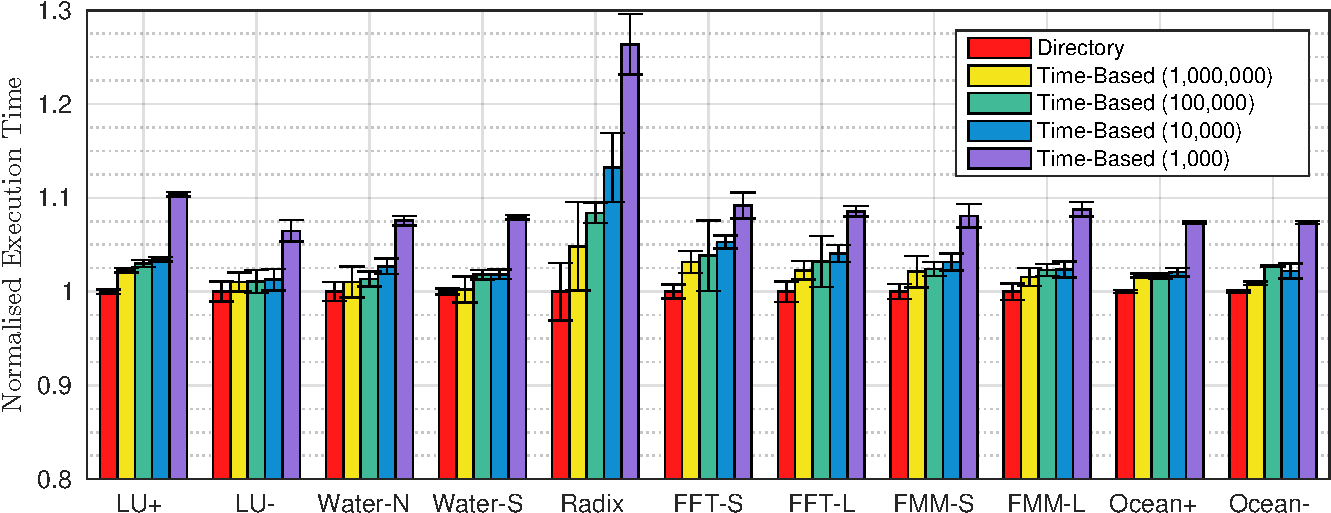
\includegraphics[width=\textwidth,height=\textheight,keepaspectratio,angle=0]{splash_combined_freebsd}}
			\caption[Splash-2 execution time, 2 software threads]{Splash-2 execution time, 2 software threads (\textit{Lower is better})} 
			\label{splash_combined}
		\end{figure}

		\paragraph{Figure \ref{splash_combined_ratio}} shows the hit/miss ratio for each coherence model. Ratios are constructed using the mean values of total hits and misses accumulated by the cache hardware counters. Note that counter values are extracted from each processor core and then combined to form one global result.
		
		\paragraph{Figure \ref{splash_combined_inv_ratio}} shows metrics specific to the architectures of directory-based and time-based models, they are not directly comparable. In the directory case, the total number of invalidation messages generated by the directory is compared to the number of messages matching a sharer cache entry (coherence address is compared with the short-tags). Matching entries are referred to as invalidate-hits, all remaining messages are false invalidates (they do not invalidate any cache lines). 
		
		In the time-based models, the number of cache misses triggered by self-invalidation are compared to the total number of cache misses.

		Directory-based coherence shows a strong overall performance. However, the best performing time-based model is within 3\% of the directory results. In 9 of the 11 tests, directory coherence shows a statistically significant performance advantage. In the remaining 2 tests (Water-N and Water-S), results displayed by the time-based model are within the standard deviation. The algorithms used in these tests require less synchronisation which is beneficial to the time-based model.
		
		Across the full range of time-based model tests, time-based (1,000,000) shows the best overall performance, supporting the general caching philosophy of exploiting spacial and temporal data locality.
		The execution time of each time-based model is directly proportional to the selected time-out value. 
		For most tests, all time-based designs fall within a 10\% range of the directory results.
		In all tests other than Radix, the models with a time-out between 10,000 and 1,000,000 cycles show a very similar execution time, often in a 2\% range.
		
		Overall, directory coherence shows a strong cache behaviour with most tests achieving a hit ratio of 92\% or more.
		False-invalidates occur when shared data is loaded and then used for some operations but never updated.
		The L2 cache maintains a strict inclusion policy, so when shared data is evicted, coherence messages are sent to all sharers. False messaging could be reduced by optimising the coherence mechanism to exploit typical memory sharing patterns \cite{Cuesta11,Cuesta13}.

		The time-based (1,000,000) model achieves better hit ratios than other time-based variants. In most tests its hit ratio is within 1--3\% of that shown by the directory. The time-based model actually shows a better hit ratio for LU-Contiguous. For the same test the directory shows its best ratio of true invalidates, indicating very efficient synchronisation. The LU test highlights the characteristics of a coherence mechanism, as high cache hit ratios do not necessarily result in a superior overall performance.
		This issue will be elaborated further in this chapter.
		
		In Figure \ref{splash_combined_ratio}, comparing (d) and (b), the time-out is increased by a factor of 100, but the hit ratio only improves by $\sim$4\%. The worst performing time-based (1,000) shows an average slowdown between 8\% and 25\%. If we ignore the slowest model, all other time-based versions fall within 3\% of the directory performance, for this configuration of benchmarks. 
		
		On the whole the slowest model demonstrates that these benchmarks require more than 1,000 cycles to perform a set of operations before synchronising or moving to a different block of data. The cost of time-counter roll-overs is also evident as memory is blocked for longer. Individual benchmark behaviour will be elaborated in further sections.

		\clearpage
		\begin{figure}[!h]
		\centering 
			\makebox{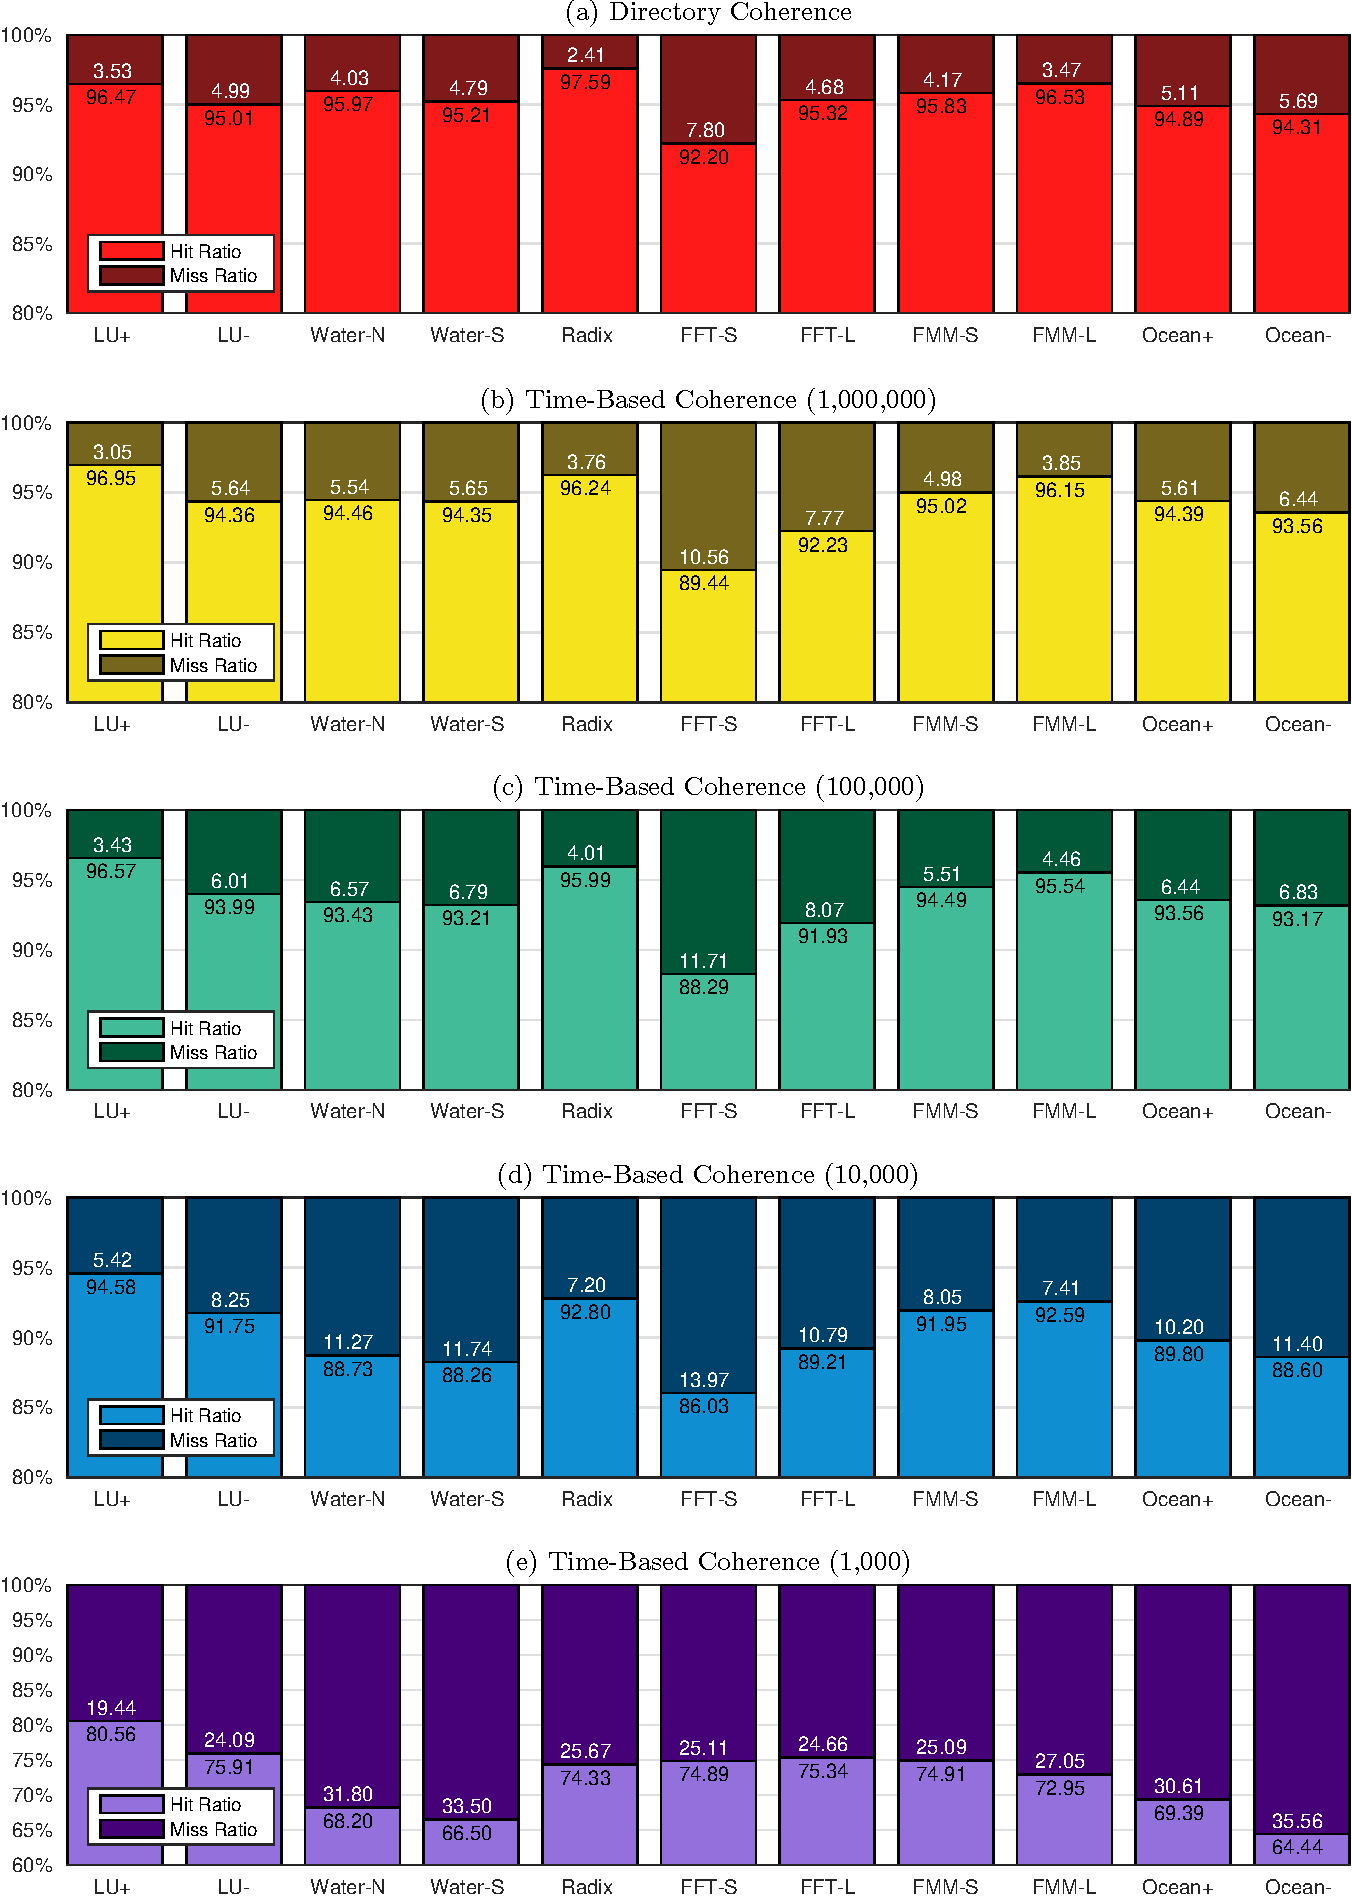
\includegraphics[width=\textwidth,height=\textheight,keepaspectratio,angle=0]{splash_combined_ratio}}
			\caption[Splash-2 hit/miss ratios]{Splash-2 hit/miss ratios. Charts (b), (c), and (d) show a similar pattern for the range of benchmarks (\textit{Note: A wider y-axis is used in (e). Charts show a ratio between total cache hits and misses, the total number of memory accesses are affected by the coherence mechanism, and may differ})} 
			\label{splash_combined_ratio}
		\end{figure}
		
		\begin{figure}[!h]
		\centering 
			\makebox{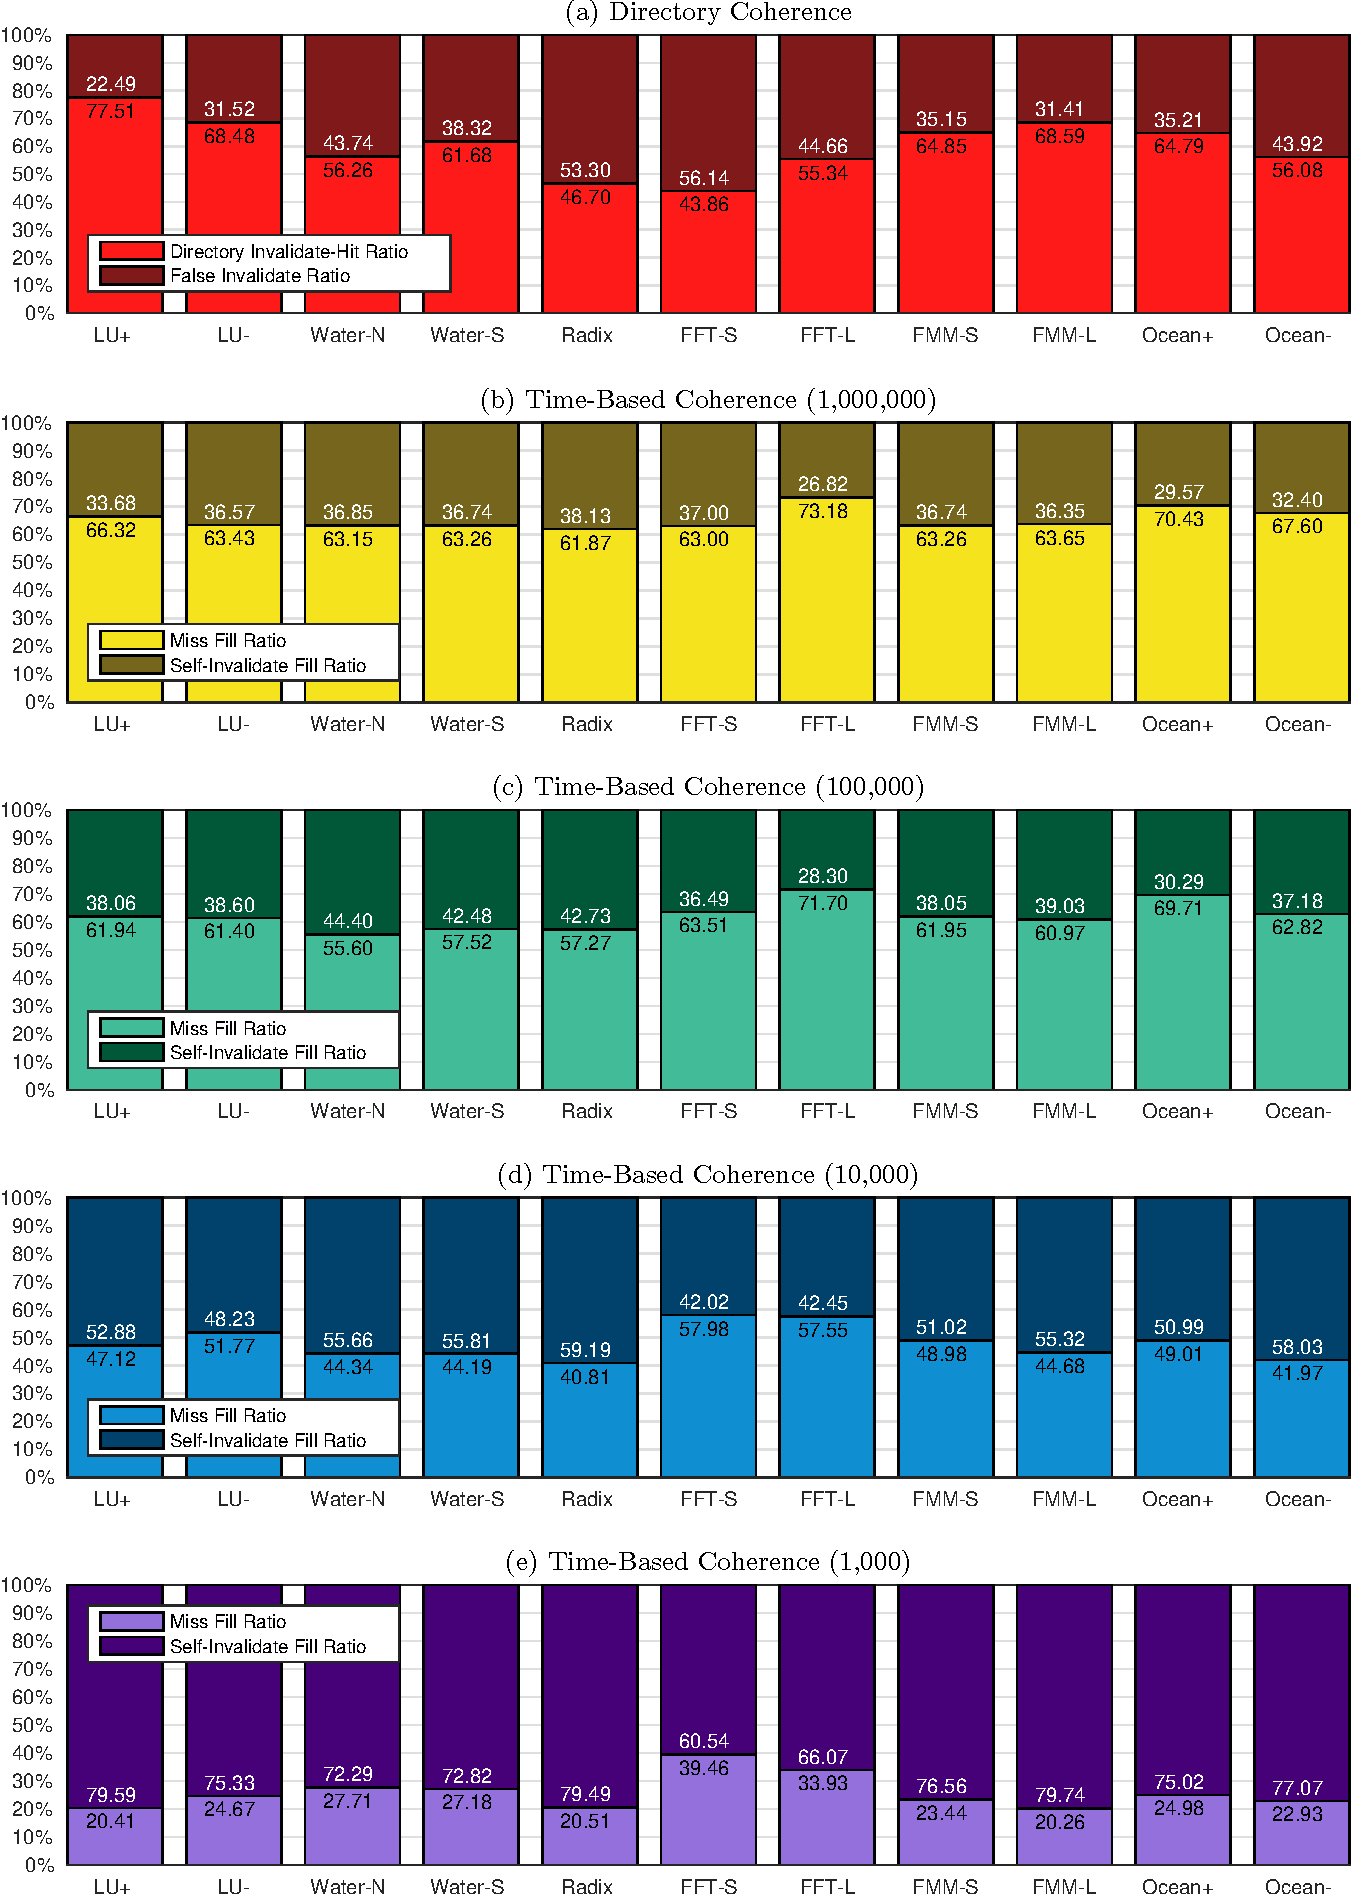
\includegraphics[width=\textwidth,height=\textheight,keepaspectratio,angle=0]{splash_combined_inv_ratio}}
			\caption[Splash-2 directory-invalidate and self-invalidate ratios]{Splash-2 directory-invalidate and self-invalidate ratios. Across the range of benchmarks, all time-based models show a similar self-invalidation pattern. (\textit{Note: Chart (a) shows invalidate messages issues by the directory in the L2 cache, (b,c,d,e) show tag-time-stamp expiry within the L1 data caches})} 
			\label{splash_combined_inv_ratio}
		\end{figure}
	
\clearpage
	\section{Optimising Time-Based Coherence}
		Prior evaluation has shown that the time-based model benefits from a longer cache time-out; fewer time-counter roll-overs. In this set of tests I evaluate cache optimisations that could improve performance.
		The benchmarks were previously tested using a software thread count of 2, in this set of tests the thread count has been increased to 16. It is a good balance between the minimum and maximum number of software threads (1--64) supported by Splash-2 tests. Results are presented in Figures \ref{splash_16thread_freebsd}, \ref{splash_16thread_hit_ratio}, and \ref{splash_16thread_inv_ratio}.
		
		Earlier tests have shown that time-based (1,000,000) model displayed the best performance of all compared time-based models. In this section I compare three BERI models: directory-based coherence, time-based (1,000,000), and time-based (1,000,000) with the polling detection [PD] (introduced in Section \ref{polling_detection_mechanism}).
		
		The time-based (1,000,000) standard model shows an improvement over the previous evaluation in Figure \ref{splash_combined} (especially LU+, Water-N, FFT-L, FMM-L, and Ocean-). The directory is affected by the increased thread count, showing a greater number of false invalidates and a marginally lower hit rate, approximately 1\%. 
		
		Time-based PD shows a more balanced performance as compared to the standard version, outperforming it outright in 5 tests. In the remaining 6 tests, the PD model shows a comparable or lower standard deviation. 
		
		The LU benchmark imposes large synchronisation overheads (Section \ref{test_settings_splash}). For 16 software threads, the time-based model shows an improved LU Contiguous execution, however, the LU Non-Contiguous results are weaker. The LU Contiguous algorithm exploits cache temporal locality by subdividing the test dataset. The Non-Contiguous version uses a coarse grained approach, which results in more communication.
		
		
		\begin{figure}[!h]
		\centering 
			\makebox{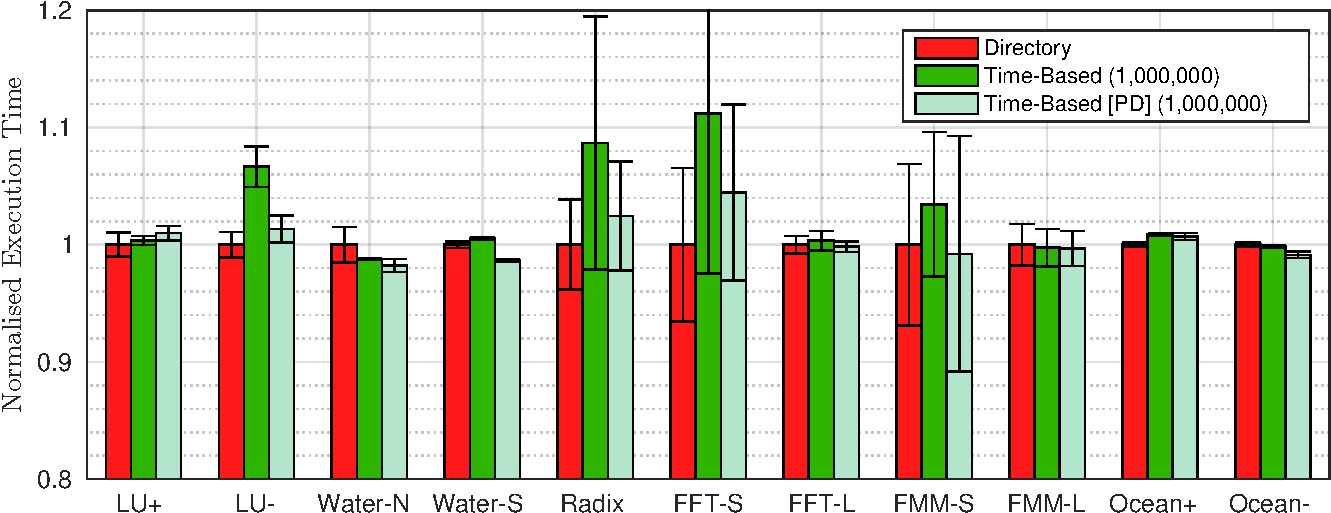
\includegraphics[width=\textwidth,height=\textheight,keepaspectratio,angle=0]{splash_16thread_freebsd}}
			\caption[Splash-2 execution time, 16 software threads]{Splash-2 execution time, 16 software threads (\textit{Lower is better})} 
			\label{splash_16thread_freebsd}
		\end{figure}
		%\vspace{-5mm}

\clearpage
		\begin{figure}[!h]
		\centering 
			\makebox{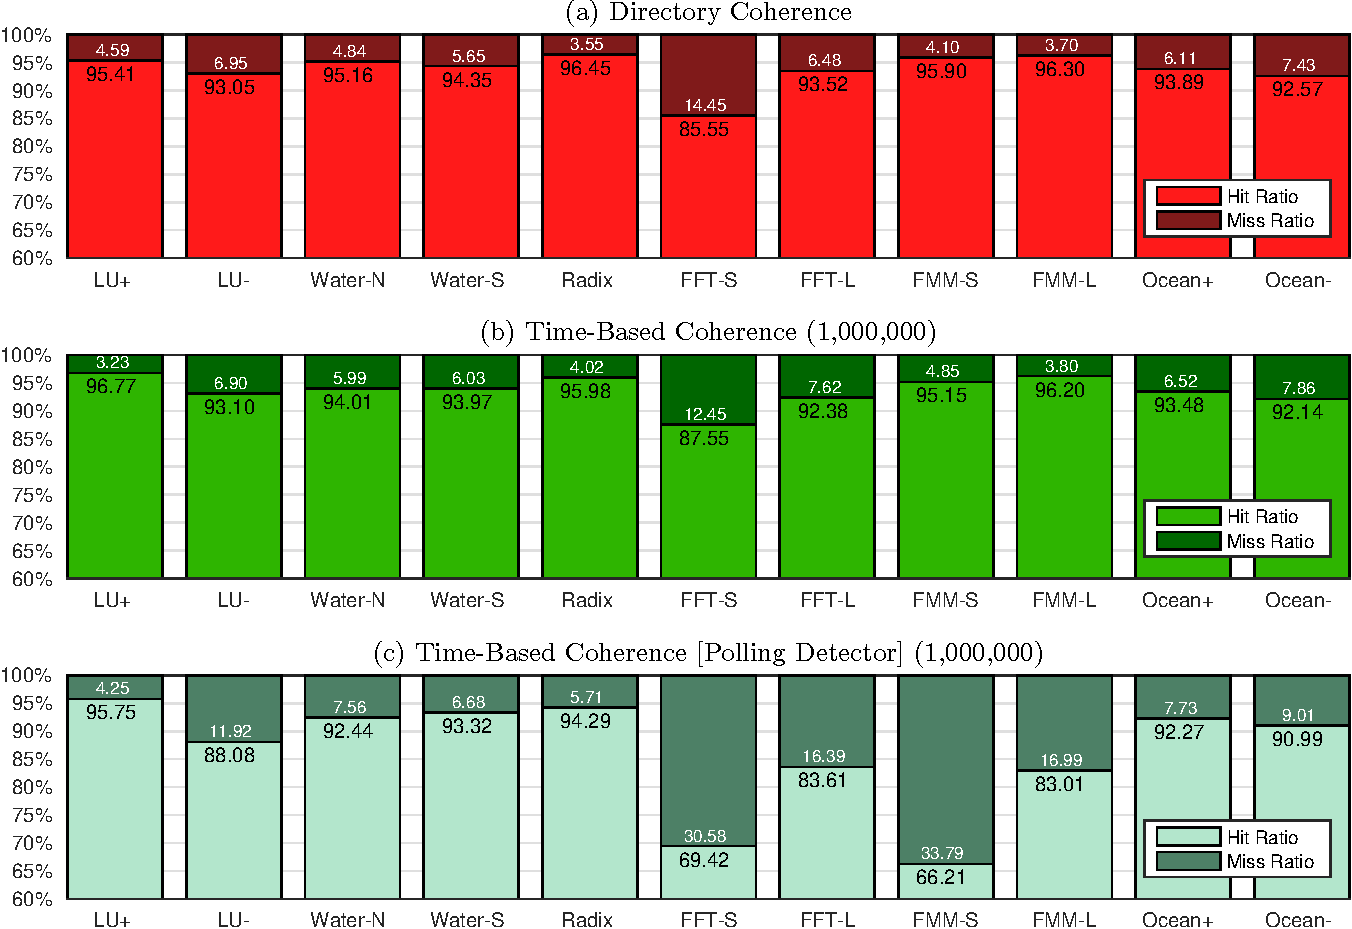
\includegraphics[width=\textwidth,height=\textheight,keepaspectratio]{splash_16thread_hit_ratio}}
			\vspace{-7mm}
			\caption{Splash-2 hit/miss ratios, 16 threads} 
			\label{splash_16thread_hit_ratio}
		\end{figure}
%\vspace{-5mm}
		\begin{figure}[!h]
		\centering 
			\makebox{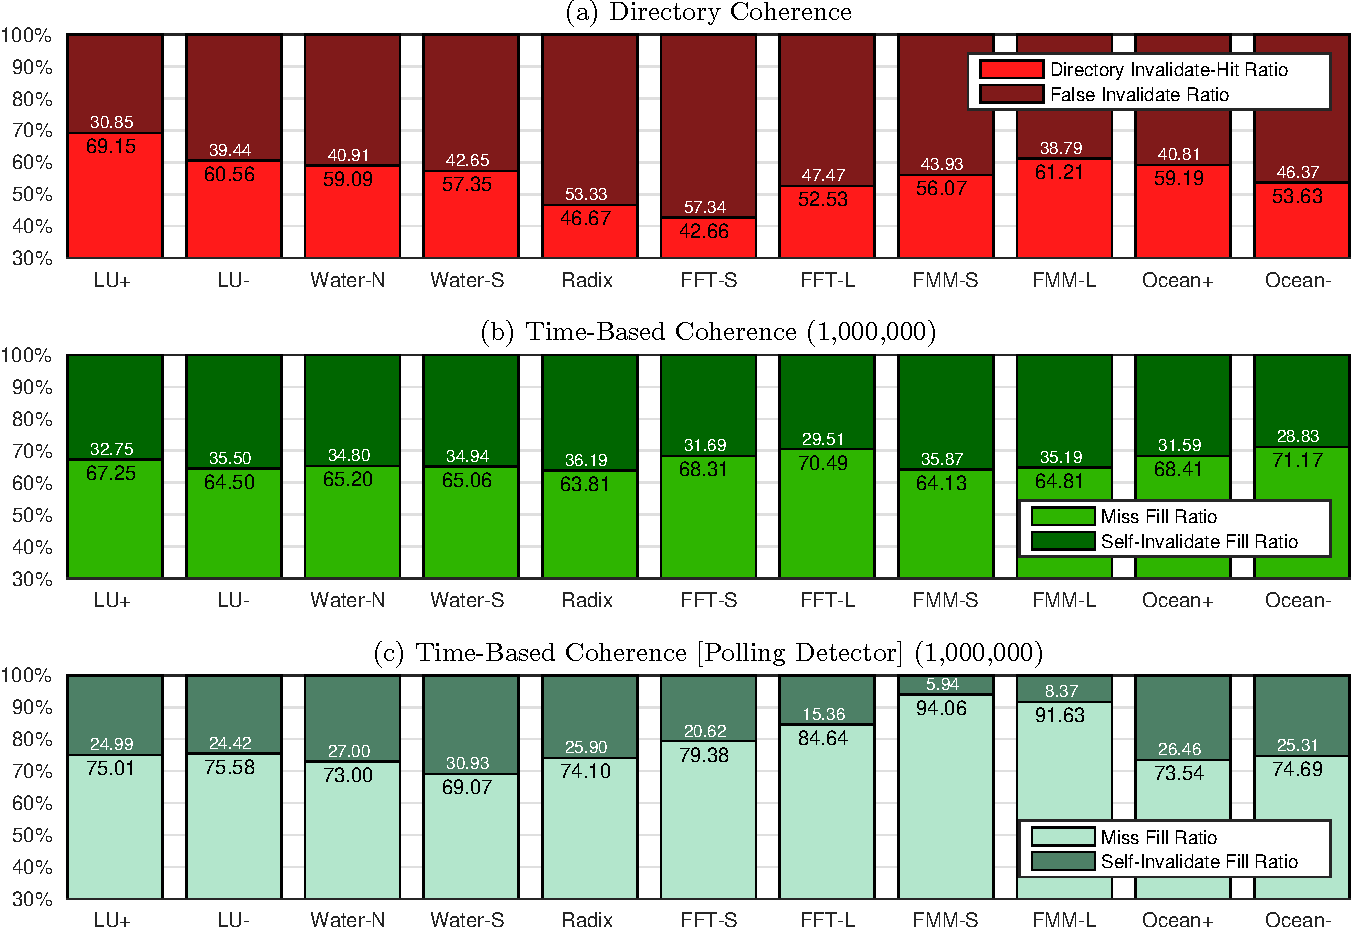
\includegraphics[width=\textwidth,height=\textheight,keepaspectratio]{splash_16thread_inv_ratio}}
			\vspace{-7mm}
			\caption{Splash-2 directory-invalidate and self-invalidate ratios, 16 threads} 
			\label{splash_16thread_inv_ratio}
		\end{figure}
\vspace{-10mm}

\clearpage
		The time-based PD version shows a much lower hit rate for LU Non-Contiguous, which results in a performance degradation. Note that the PD version shows lower hit rates for all benchmarks, but a better self-invalidation ratio, since misses due to polling detection are not counted. 
		
		The Water benchmarks are designed to reduce overall coherence communication and synchronisation. Both time-based models respond positively to this test, with the PD model showing a $\sim$2\% improvement over the directory. 
		
		The Radix test uses a bursty communication pattern and a constantly varying dataset size. Both factors negatively affect the time-based model as time-counter roll-overs are more frequent than in other tests. A larger tag-time-stamp is likely to improve performance. The PD model responds much better to Radix than the default design.
		
		FFT-Small forces more communication due to a smaller a dataset and partitions, whereas FFT-Large will cause shared memory penalties due to L1 capacity misses. The latter allows time-based coherence to show a better baseline relative performance. The small version of this test severely penalises the time-based model, despite showing a better hit rate than the directory. The PD model shows a much lower hit rate, but also fewer self-invalidates indicating polling detection.
		
		For FMM Small and Large, the PD model shows its best self-invalidation ratio, but a weaker overall hit ratio due to polling detection. The directory design suffers due to the coherence communication overheads imposed by this test.
		
		For both Ocean benchmarks the time-based designs perform better than the 2 thread evaluation. A significant proportion of memory references are shared and all models demonstrate a similar behaviour and cache hit ratios.
		

	\section{Extended Splash-2 Comparison}
		In this section the performance of time-based coherence is analysed using a range of Splash-2 test parameters. Five tests are used in this evaluation: both LU, Radix, and both Ocean tests. These tests should provide sufficient evidence to understand the coherence behaviour. In each test, two main parameters are varied: dataset block size and software thread count. Figures \ref{splash_extended_polling} and \ref{splash_extended_standard} show the obtained results. The directory results are shown as a flat baseline.
		
		The time-based PD model consistently outperforms the standard version. It is also clear that an increase in block size (reduction in synchronisation) yields better performance. Execution time rises with an increase in software thread count. Note that in the Ocean Contiguous evaluation, the grid size value of 10 is insufficient for testing 32 and 64 threads.
		
		This experiment shows that the polling detection mechanism is still useful in parallel applications that largely depend on locks and barriers. These results also confirm my predictions of the drawbacks of the current time-based model. They can be reduced by either increasing the TTS size or using a different technique for triggering time-outs.

		\paragraph{Figure \ref{splash_extended_standard} --} Time-based coherence 1,000,000.
		\begin{description}
			\item [(a) LU Contiguous] An increase in thread size negatively affects the coherence behaviour as more synchronisation is necessary. However, a larger workload compensates for this overhead and produces a close to baseline performance. A small dataset is severely affected by an increase in thread count.
			\item [(b) LU Non-Contiguous] This test displays a similar behaviour to that shown in (a), but in this test the performance impact of a small dataset is lower. Also, a similar response to software threads is observed.
			\item [(c) Radix] This test has shown the largest performance overheads for the time-based model in all previous evaluations. The coherence model responds negatively to both the dataset size and thread count. For 64 threads and a 1024 Radix, the performance is almost 50\% worse than the directory equivalent. 
			\item [(d) Ocean Contiguous] Similar to the tests discussed above, this Ocean benchmark displays a higher coherence overhead for smaller datasets. The overheads for software threads are reasonable for up to 8--16 threads, but rapidly increase for 32 or more. The time-based model actually performs better than the directory for the default test grid size of 258. 
			\item [(e) Ocean Non-Contiguous] The results are similar to those shown in (d), however, this test shows better scalability for 32 and 64 threads.
		\end{description}
		
		\paragraph{Figure \ref{splash_extended_polling} --} Time-based coherence 1,000,000 with memory polling detection. The individual test behaviour is almost identical to the standard time-based model, but the execution time for each test variant in lower. All of the tests execute faster for smaller datasets. The execution time for Radix and Ocean tests running 32--64 threads is almost 25\% better than the standard model.
		
		This test demonstrates that the time-based model can be significantly improved through optimisations such as the polling detection mechanism. While the performance for small datasets is poor relative to the directory, memory hungry tests can benefit from this model.

\clearpage
		\begin{figure}[!h]
		\centering 
			\makebox{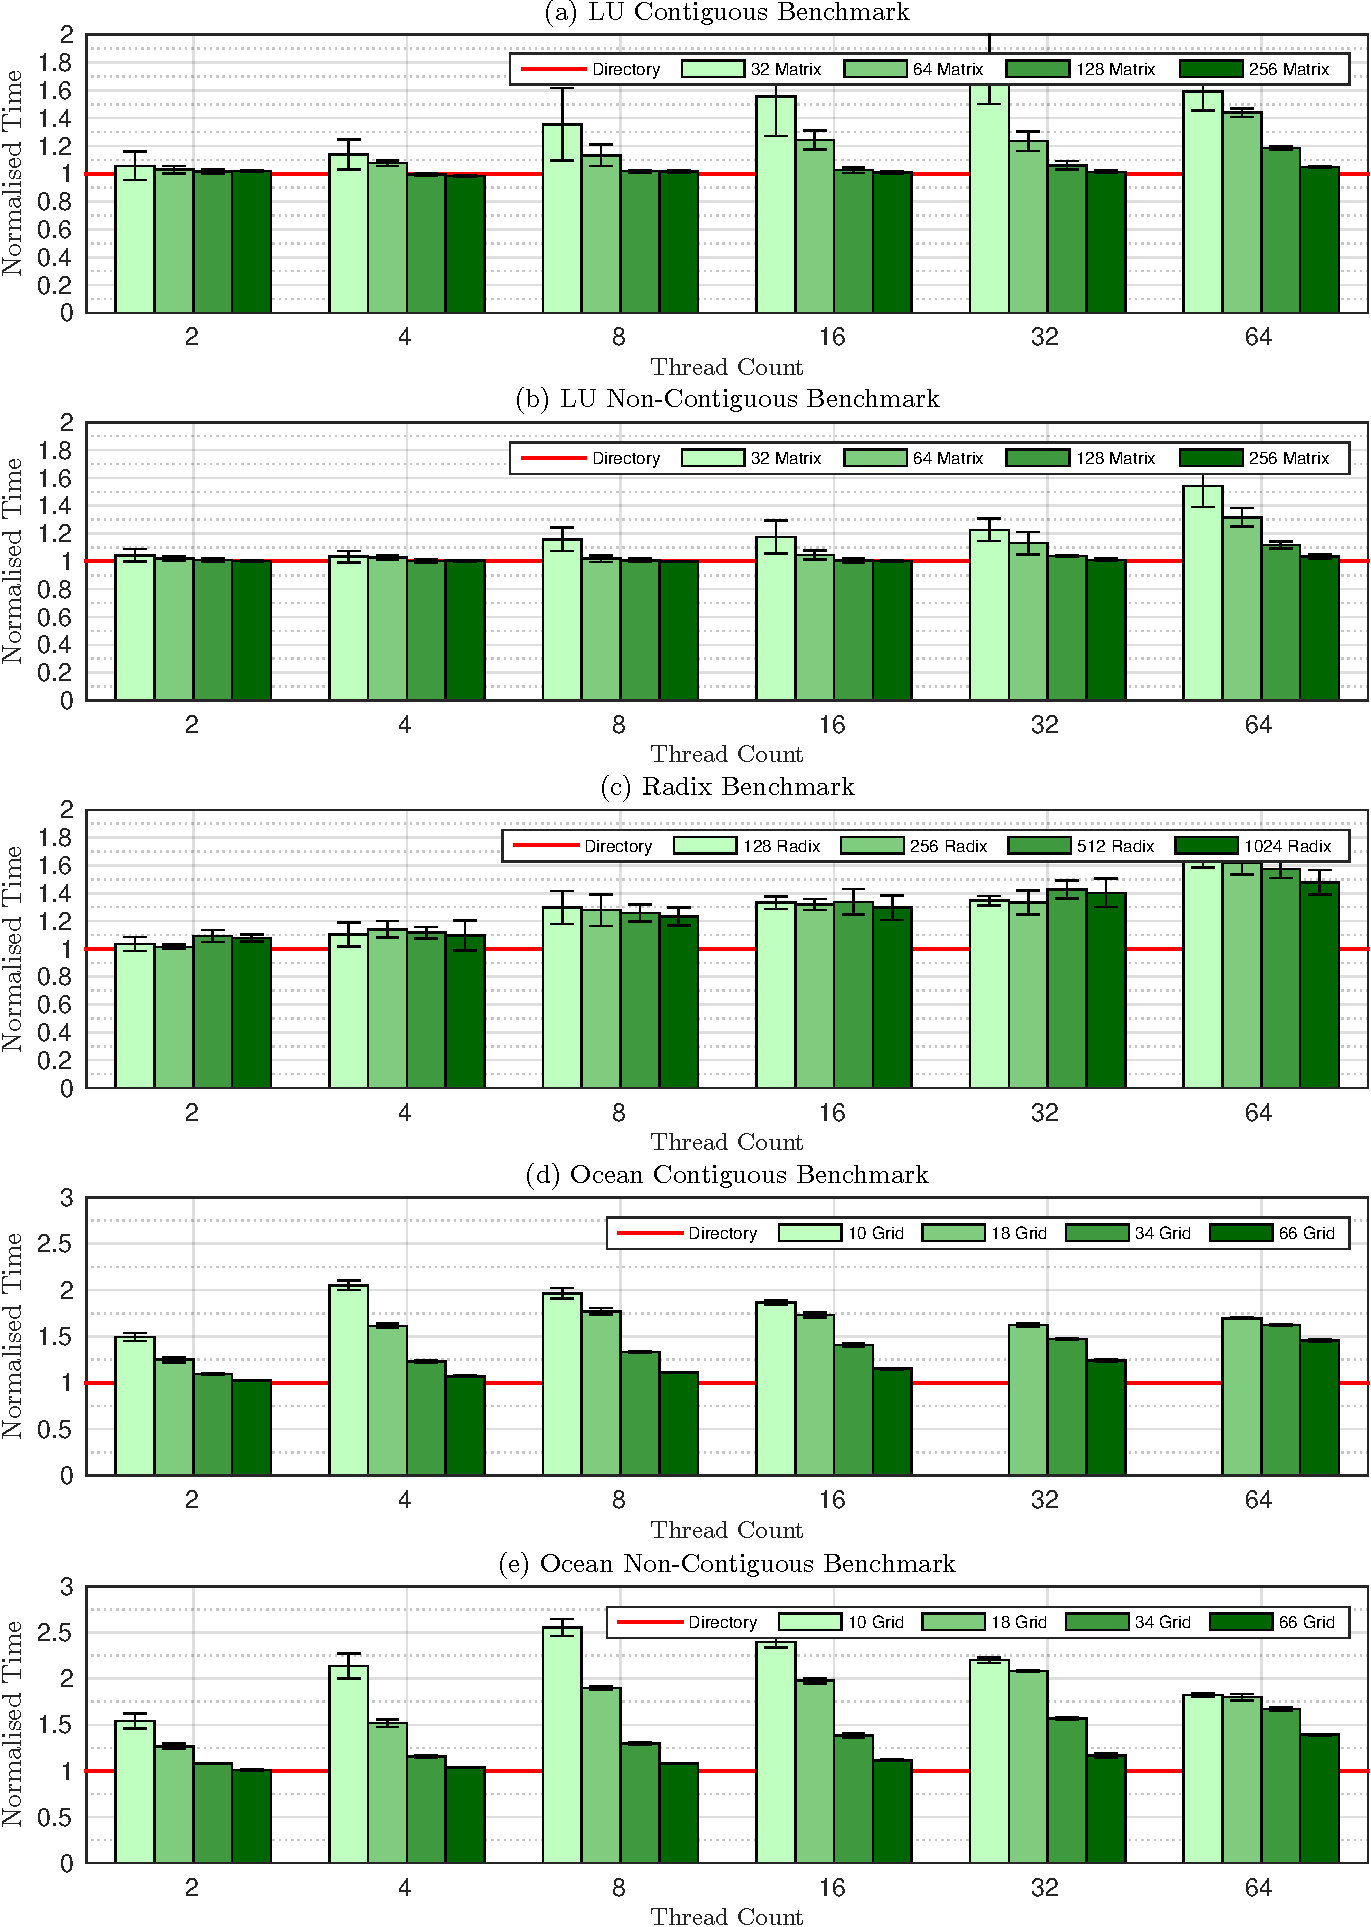
\includegraphics[width=\textwidth,height=\textheight,keepaspectratio,angle=0]{splash_extended_standard}}
			\caption[Splash-2 extended benchmarks, part 1]{Splash-2 extended benchmarks, time-based coherence 1,000,000 (\textit{Note: Each chart shows the total execution time taken per evaluation parameter, normalised using the mean baseline established by the BERI Directory model. The thread count represents the number of software threads spawned by each benchmark})} 
			\label{splash_extended_standard}
		\end{figure}
		%\vspace{-5mm}

		\begin{figure}[!h]
		\centering 
			\makebox{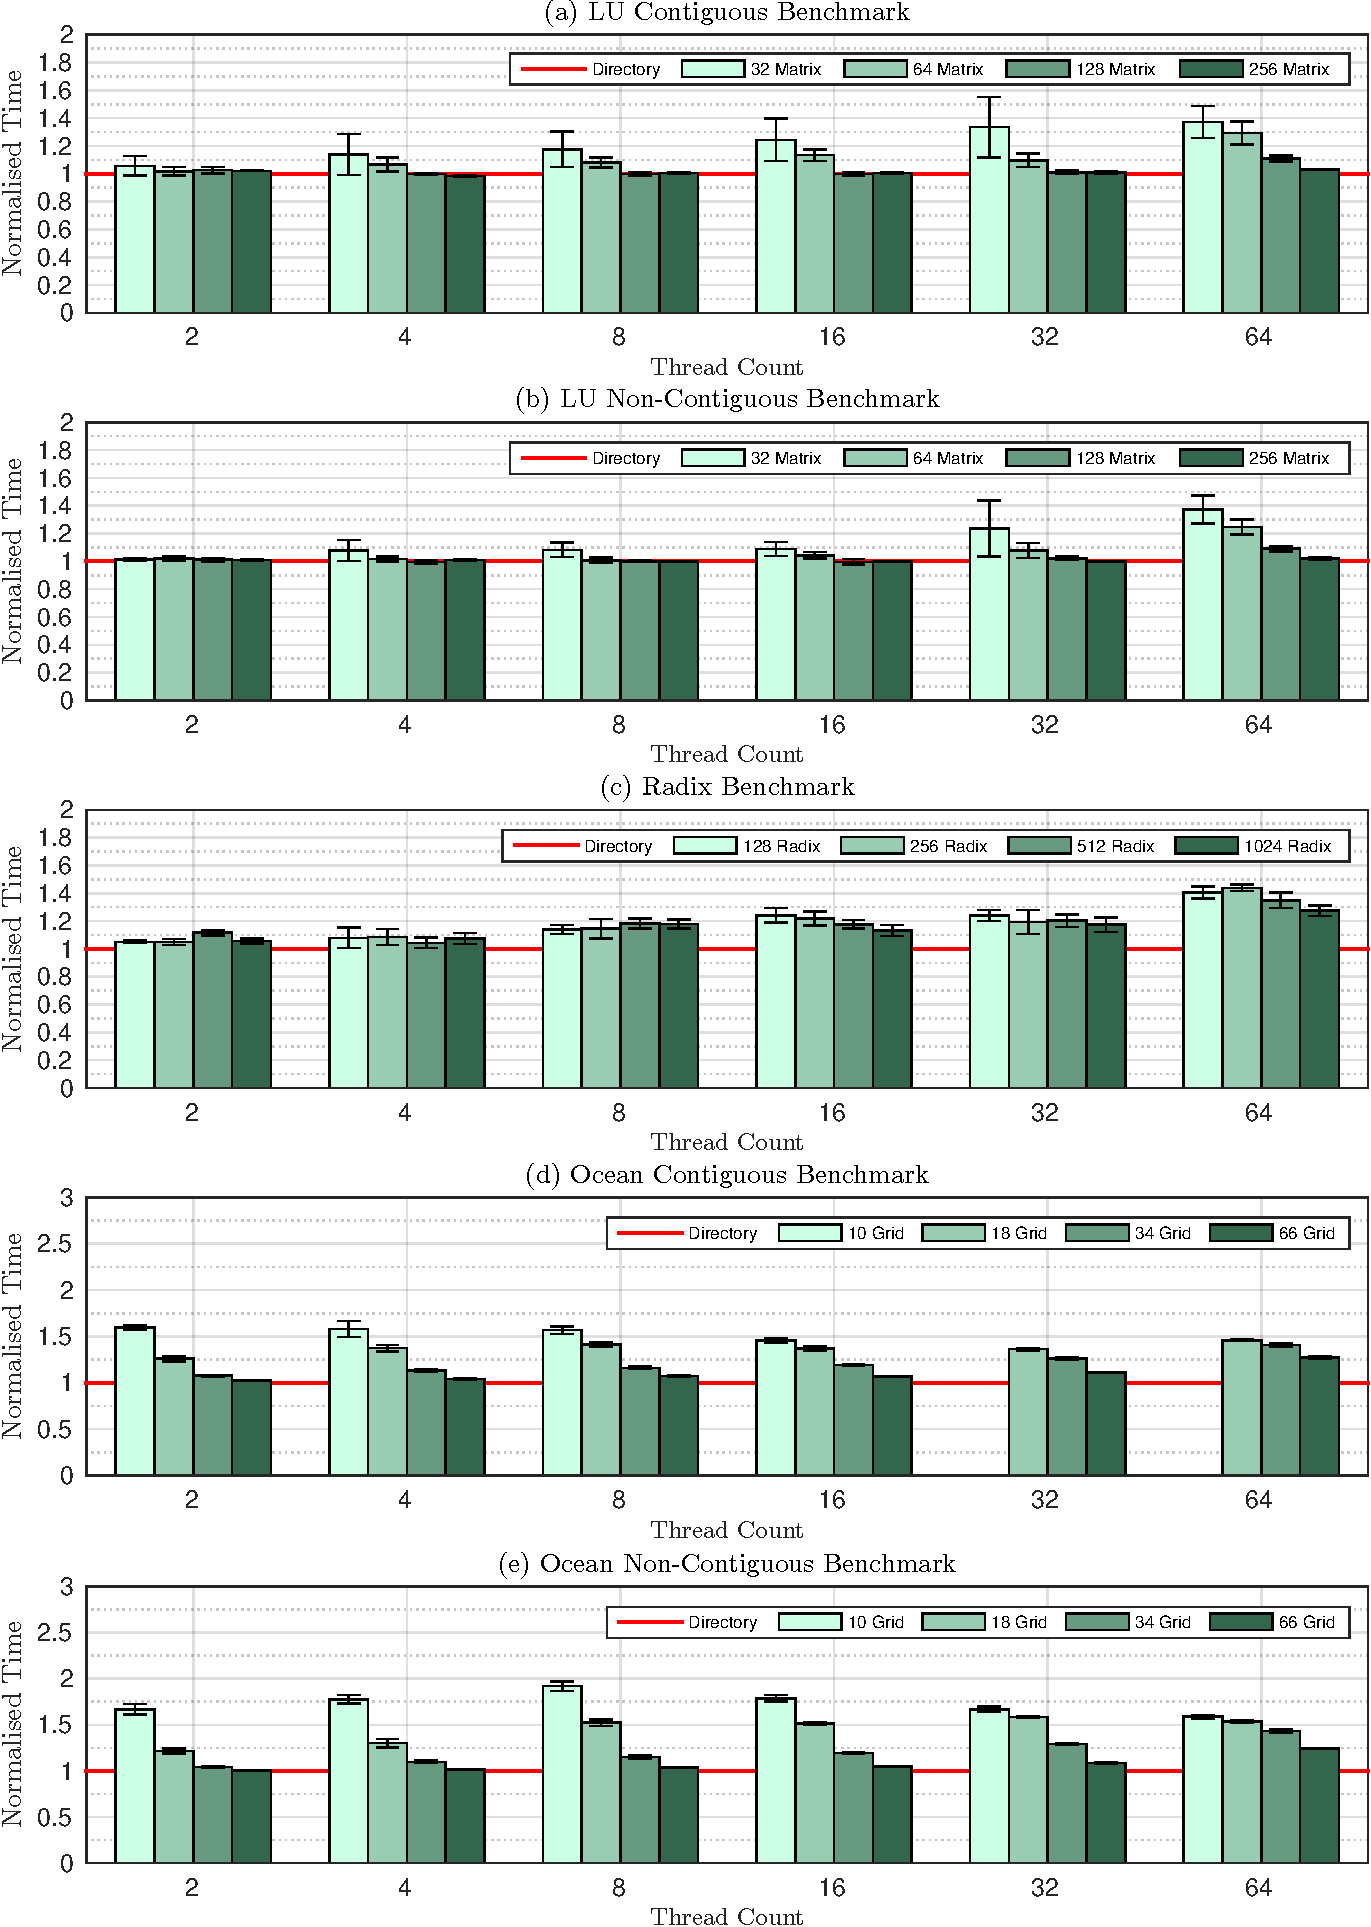
\includegraphics[width=\textwidth,height=\textheight,keepaspectratio,angle=0]{splash_extended_polling}}
			\caption[Splash-2 extended benchmarks, part 2]{Splash-2 extended benchmarks, time-based coherence 1,000,000 with memory polling detection (\textit{Note: Each chart is compared against the mean execution time of the BERI Directory model, same baseline as shown in Figure \ref{splash_extended_standard}. The Ocean benchmarks are displayed using a different scale})} 
			\label{splash_extended_polling}
		\end{figure}
		%\vspace{-5mm}	
		

\clearpage
	\section{Effects of Cache Size on Performance}
		In this section I evaluate the performance variations arising from changing the cache size; the cache design is not altered. 
		I am interested in understanding whether an increase in either to L1 or L2 cache size will adversely effect the performance of the BERI coherence mechanisms, time-based in particular. 
		One disadvantage of the current version of the time-based coherence model is that time-counter roll-overs cause cache reinitialisation; effectively a slow cache flush. This property has not shown a significant disadvantage in the default tests, however, an increase in the L1 size will increase the overheads of reinitialisation; a larger cache leads to a longer blocking time.
		
		The directory model may also be affected by the increase in either the L1 or L2 size, since a bigger L1 will force greater L2 inclusion and potentially a higher capacity miss rate. A larger L2 will likely improve the outcome, as capacity misses will reduce, thus reducing the number of forced coherence messages. Larger L1's may actually have a negative effect as they will cache more data, so the directory will likely need to track more shared data, leading to higher coherence messaging due to L2 capacity misses.
		
		I am also testing a design where both L1 and L2 are increased in size. Note that only the L1 data cache is increased and the L1 instruction cache is kept constant throughout. A total of 8 models are tested using the same benchmark settings as shown in Figure \ref{splash_16thread_freebsd}, 16 software threads. The BERI directory and BERI time-based polling detection (1,000,000) are compared to three variants: double L1 size, double L2 size, and double L1 and L2 caches.

		\begin{figure}[!h]
		\centering 
			\makebox{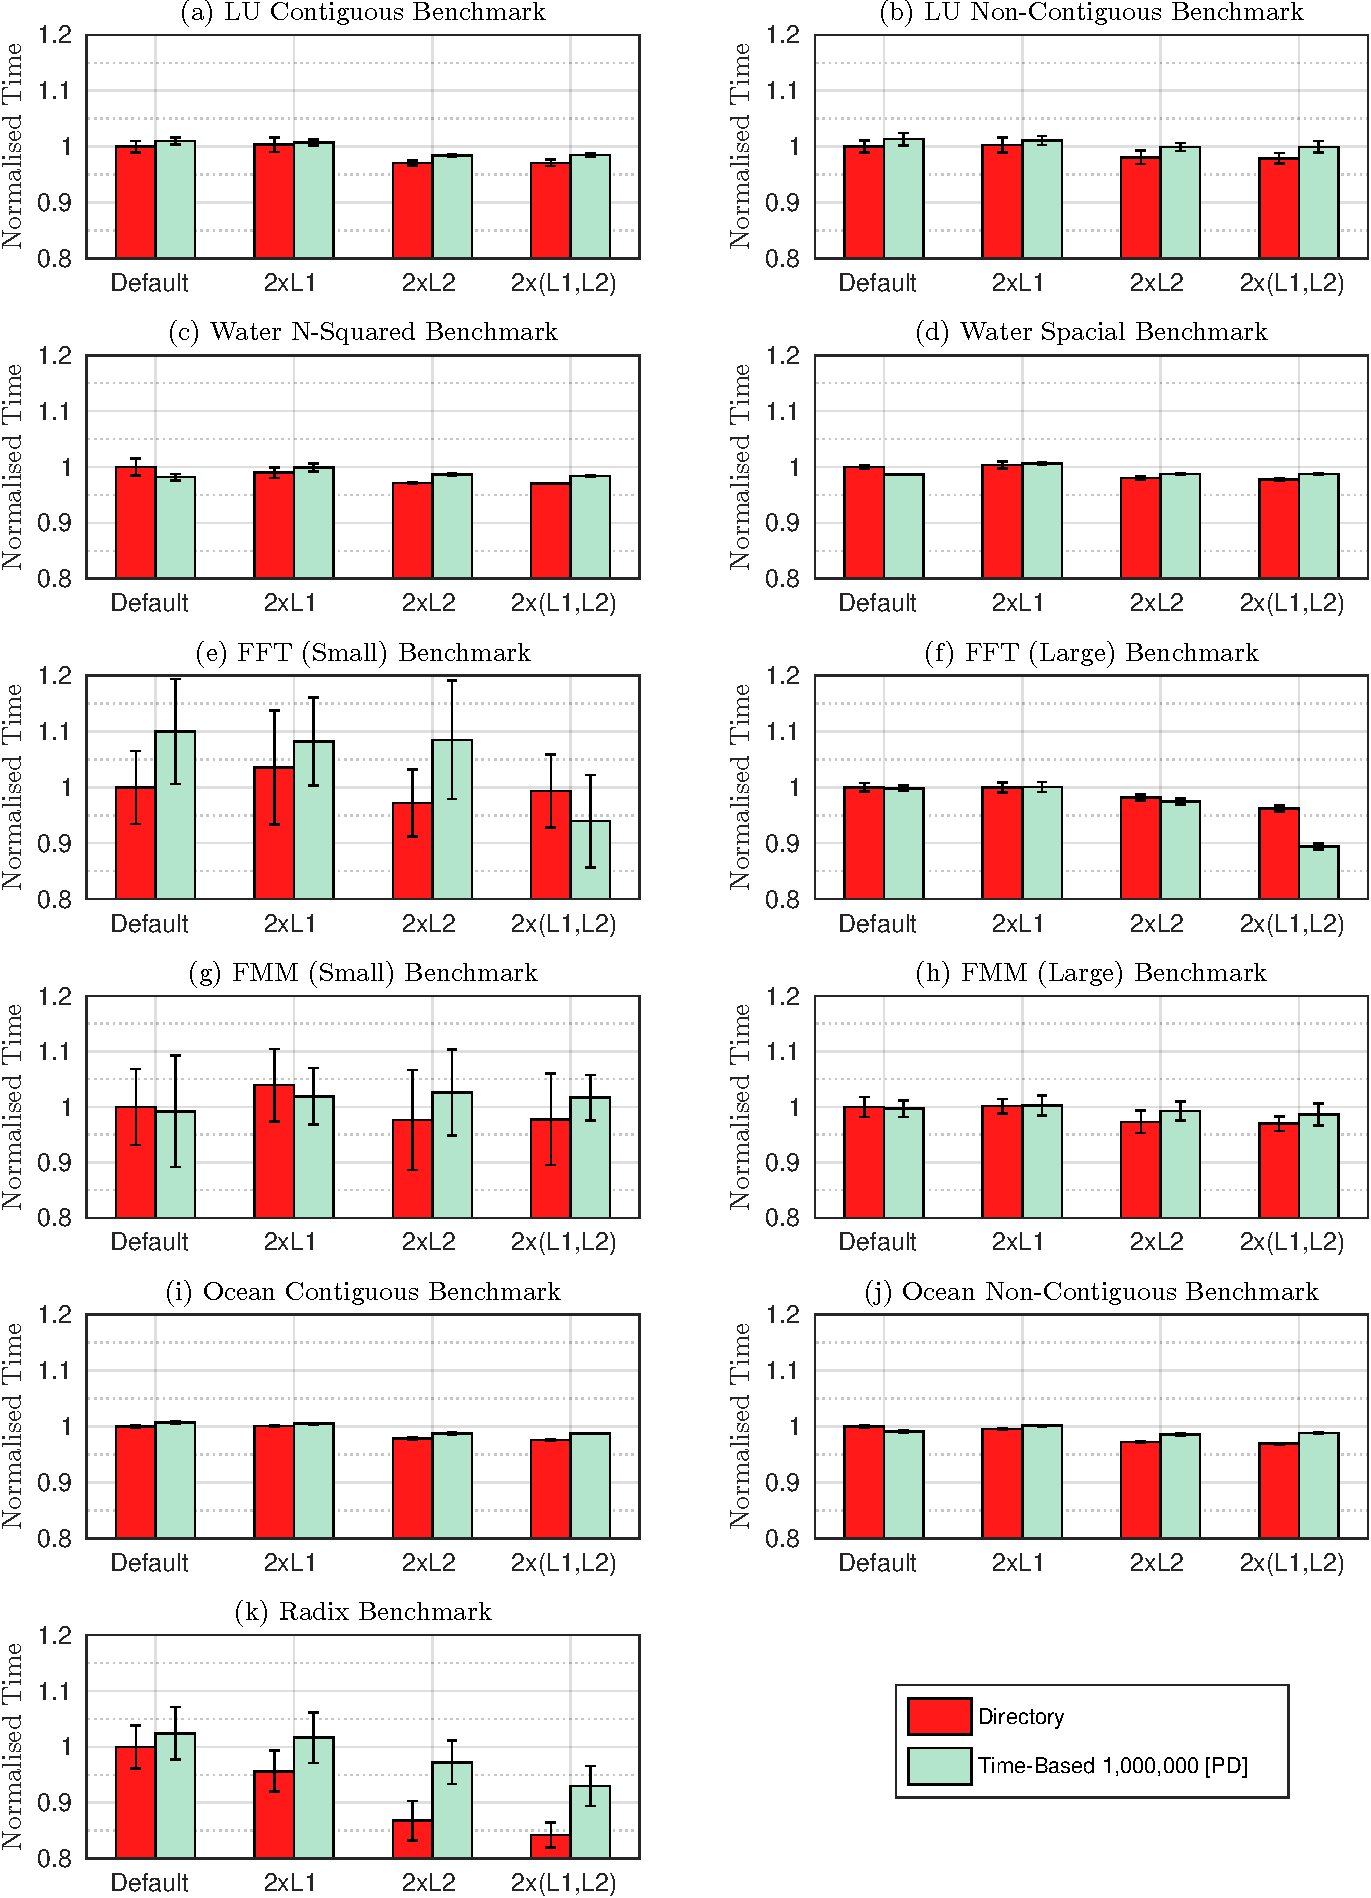
\includegraphics[width=\textwidth,height=\textheight,keepaspectratio,angle=0]{splash_big_cache_full}}
			\vspace{-3mm}
			\caption[Splash-2 cache size vs. coherence]{Splash-2 cache size vs. coherence (\textit{Note: Each test is evaluated using the default benchmark parameters and 16 threads, as stated in previous sections. All tests results are normalised relative to the default directory evaluation})} 
			\label{splash_big_cache_full}
		\end{figure}

		\begin{description}
			\item [(a) LU Contiguous] The directory and time-based models show a similar response in the default and 2xL1 tests. Doubling the L1 caches does not benefit either model. Both models show an improvement in the 2xL2 and 2x(L1,L2) tests, however, the directory gains a bigger advantage. This is likely due to a reduction in invalidates as shared line evictions are reduced in the L2 cache.
			\item [(b) LU Non-Contiguous] Both models show a similar pattern to that demonstrated in (a). Neither model is penalised by the changes in cache size. The time-based model improves with an increase in the L2 cache size but the directory shows a better improvement.
			\item [(c) Water N-Squared] In this test the directory model shows a steady improvement with a size increase in any of the caches. The time-based model holds an advantage in the default case but shows weaker performance once the L1 cache size is increased, likely due to a larger time-counter roll-over overhead. An increase in the L2 size improves over the 2xL1 case, however, none of the results quite match the default case.
			\item [(d) Water Spacial] This test demonstrates an almost identical behaviour to that of Water N-Squared.
			\item [(e) FFT-Small] In this test the directory model is penalised whenever the L1 cache size is increased. More data is privately cached which then results in L2 capacity misses and additional coherence messaging. The best performance is shown when only the L2 size is increased, supporting the reasons mentioned above. The time-based model shows some improvement over the default in both the 2xL1 and 2xL2 tests. This test produces a wide range of results, as illustrated by the standard deviation. Interestingly the combination of a larger L1 and L2 results in a significant improvement.
			\item [(f) FFT-Large] The relative performance of the time-based model is much better than in (e). A larger data block size causes fewer synchronisations, benefiting the time-based model. The directory response to an increased L1 is less dramatic; a larger data block size reduces the number of capacity misses, as blocks are not constantly replaced in the L2.
			\item [(g) FMM-Small] The directory is heavily penalised in the 2xL1 case, similar reasons to (e). A larger L2 cache rectifies the performance drop. The time-based model appears to be penalised when either the L1 or the L2 are increased, however, the block size of this test is small so the behaviour is unpredictable due to frequent synchronisation operations. Note the standard deviation for both models, the results show a significant overlap for every cache configuration.
			\item [(h) FMM-Large] Similar to the transition in FFT from Small to Large, this test also shows more stable results as compared to (g). The directory only improves when the L2 cache is increased. The time-based model shows a similar behaviour but loses out to the directory for both 2xL2 and 2x(L1,L2) tests.
			\item [(i) Ocean Contiguous] This test is likely to cause substantial capacity and conflict misses, as a result both coherence models show an improvement when the L2 cache size is increased. The overall performance improvement of the directory model is marginally better.
			\item [(j) Ocean Non-Contiguous] In this test the time-based model is better in the default case, however, it is penalised by an increase in L1 size. This is visible in both 2xL1 and 2x(L1,L2) tests. The test generates a large number of shared memory references and fast coherence communication benefits the directory model.
			\item [(k) Radix] This test shows the most drastic change in relative performance between the two models. It also confirms the previous observations of this test, which have shown that the time-based model suffers serious overheads. On every iteration the sorting algorithm builds local data clusters which are later merged and redistributed. This generates bursty synchronisation traffic that penalises the time-based model. However, both models show a significant improvement with an increase in any cache size, more than any other test in this set-up. This further proves that more cache spaces allows local Radix histograms to be stored and immediately reused, while capacity misses would result in frequent requests to main memory which are costly.
		\end{description}


%\clearpage
\section{Evaluating FreeBSD Commands}
	\label{results_polling}
	
	The purpose of these tests is to demonstrate that the time-based coherence model does not adversely affect single-threaded performance. Some common command line applications available in FreeBSD have been tested. These commands are single threaded, so instead of testing shared memory interactions, we observe any shortcomings or pitfalls in the behaviour of time-based coherence. Note that the OS is concurrently executed and some scheduler interference is expected. Each test run is sampled a minimum of 10 times.
	
	Communication centric coherence schemes should have little or no effect on single threaded applications as no shared memory interactions occur, hence, no coherence messaging is required. The strict inclusion policy required in the BERI directory coherence scheme could still impact the overall performance, as accurate directory tracking may produce false coherence messages.
	
	The automatic self-invalidations in the time-based coherence scheme will likely affect the performance of these applications. In fact, self-invalidates are shown to be useful and necessary for the given set of applications. I have developed the memory polling detection (PD) scheme specifically due to the preliminary evaluation of these applications. The effect is most significant in the CP test where the standard and PD versions show a dramatic performance difference, the standard version is up to 4 times slower than the PD model. This will be discussed in more detail in Section \ref{results_cp}.
	
	The tests results show that the time-based coherence model does affect single threaded programs as hypothesised, however, the models with PD or lower time-out values, usually fall within 10\% of the directory results. The advantages of directory coherence are evident in these examples and further improvements in polling detection could benefit the time-based model. Identifying sharing patters, producer-consumer relations, and other memory behaviour profiling is often used for optimising coherence schemes \cite{Byrd99,Lilja93,Sanchez12,Cuesta11}.

%\clearpage
	\subsection{DD}
		\label{results_dd}
		The (dd) application is one of the common commands used for copying disk blocks on UNIX and UNIX-like systems. This command can be used to access hardware device and special device files, such as /dev/zero, /dev/null and others. Command line arguments such as block size and count are used to dictate the number of bytes that are loaded, stored, or converted.
		
		A simple test has been constructed based on (dd). The test performs a load and store operation from /dev/zero (device producing zero value bytes) to /dev/null (device consuming all values stored to it). Time taken for this operation is recorded for a range of input arguments. 
		
		Two major input parameters of DD are varied: block transfer size and the block count. The total amount of data transferred is varied from 1K bytes to a maximum of 100M bytes. Count values are different for each block size, as larger blocks will require fewer transfer increments. The count values are scaled by a factor of 10 until the maximum total transfer is achieved. 
		Test input data is sourced from /dev/zero since other sources such as /dev/random often add overheads due to arithmetic operations.
		
		\begin{figure}[!t]
		\centering 
			\makebox{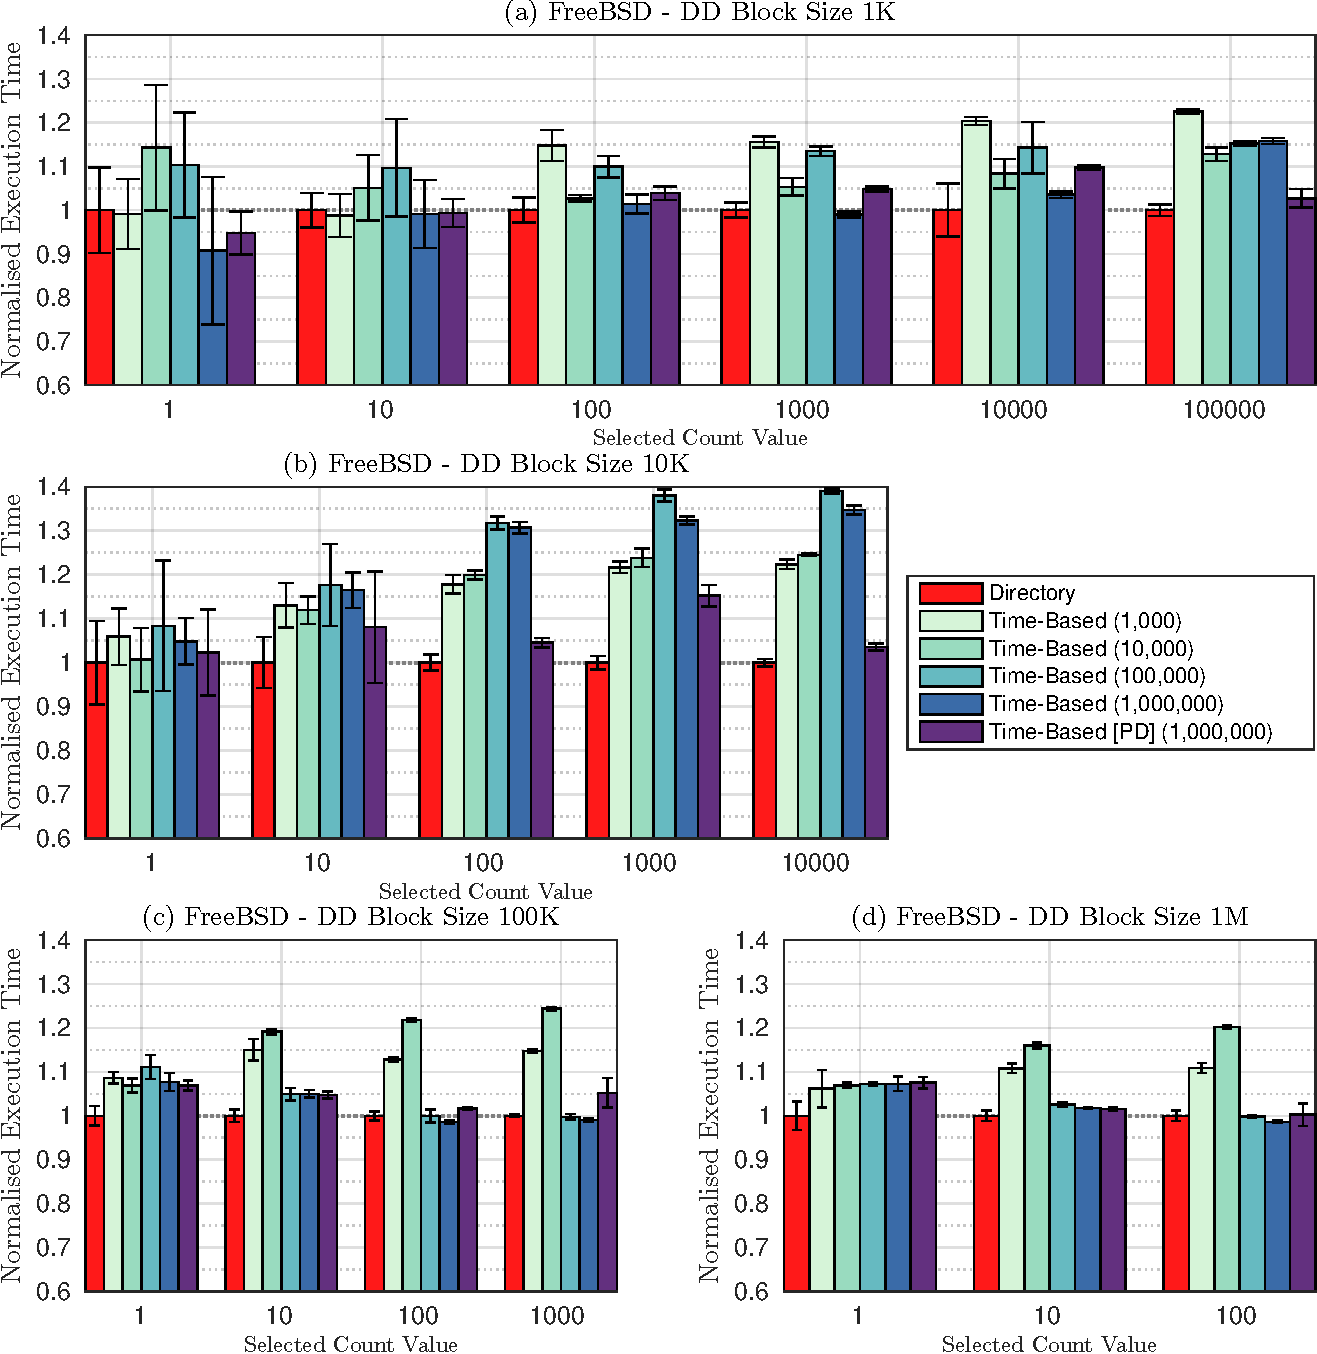
\includegraphics[width=\textwidth,height=\textheight,keepaspectratio,angle=0]{dd_freebsd_full}}
			\caption{FreeBSD DD performance evaluation} 
			\label{dd_freebsd_full}
		\end{figure}
		
		The results (Figure \ref{dd_freebsd_full}) show that there is no distinct pattern between the time-based models across all test variants. However, for a given block size the behaviour is somewhat consistent. The PD scheme is consistent throughout the range, falling within 10\% of the directory execution time in all but one test.
		
		In test (a), all time-based models fall within 20\% of the baseline, with the standard (1,000,000) model performing better than PD in most cases. In test (b), the PD version is more consistent in its execution time and shows the best overall performance. Similar behaviour is observed in tests (c) and (d). 



%\clearpage	
	\subsection{CP}
		\label{results_cp}
		The file copy (cp) command is similar to (dd), however, it offers a higher level of abstraction and deals with files and directories rather than disk blocks. The test crafted based on the (cp) command deals with a fixed set of files ($\sim$100K, $\sim$1M and, $\sim$2M) and copies them between directories. The test performance is measured using hardware registers.
		
		\begin{figure}[!ht]
		\centering 
			\makebox{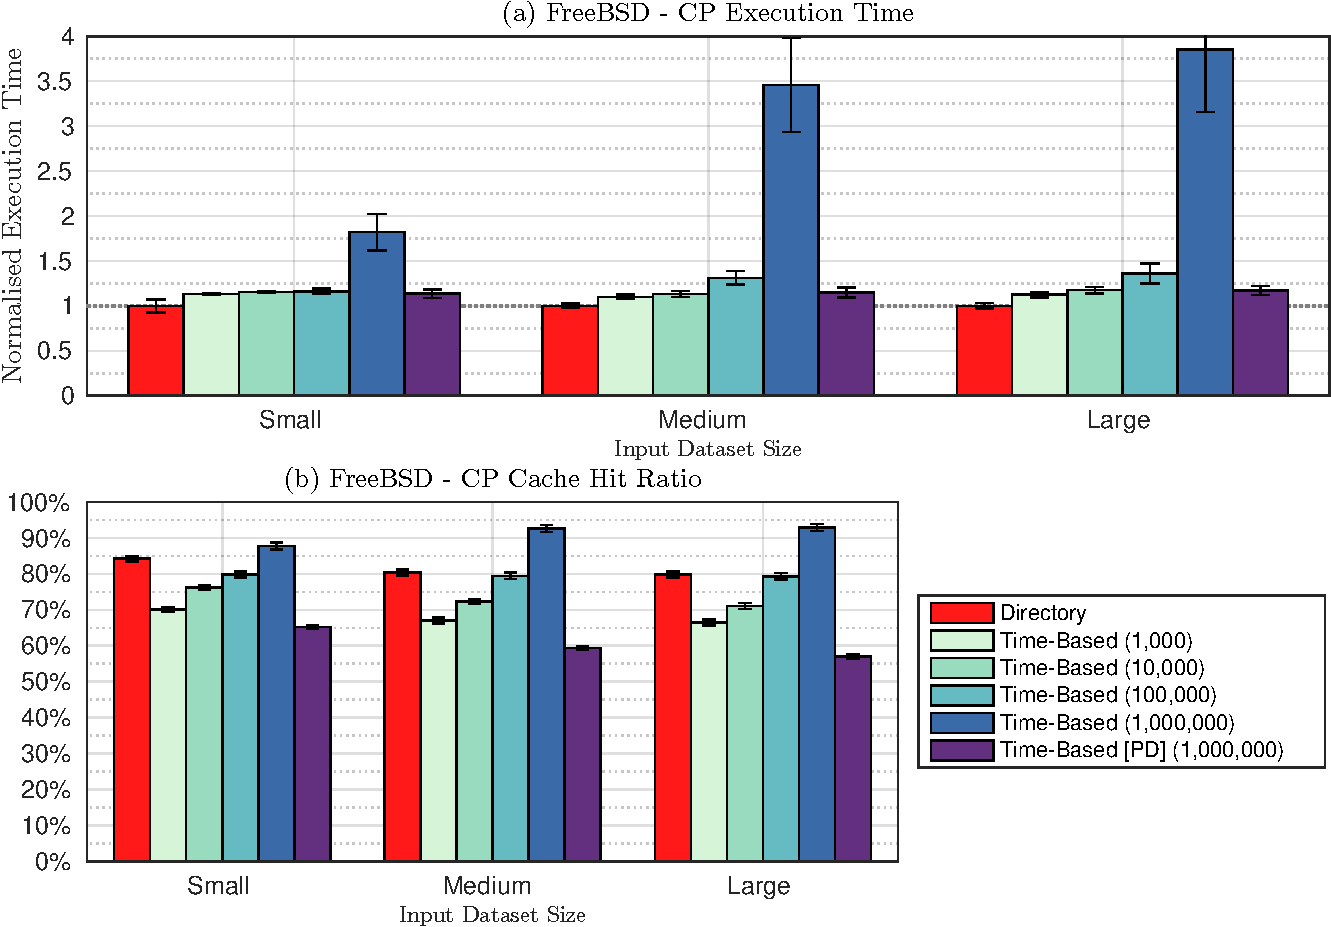
\includegraphics[width=\textwidth,height=\textheight,keepaspectratio,angle=0]{cp_freebsd_full}}
			\caption{FreeBSD CP performance evaluation} 
			\label{cp_freebsd_full}
		\end{figure}
		
		This application actively uses SYNC instructions, however, it still relies on memory polling. It is particularly evident from the exponential increase in execution time when comparing the 100,000 and 1,000,000 time-based models. The increasing standard deviation of the 1,000,000 model also suggests that some time-outs occur at favourable synchronisation boundaries, yielding a better execution time. This test was the primary cause for developing the hardware polling detection mechanism in the L1 data caches.
		
		Note the relatively low hit rate of the PD mechanism as compared to other schemes. In this experiment a higher miss rate in the time-based scheme is actually a positive indicator. It demonstrates that actively polled lines are refreshed. The directory uses coherence messages to update stale data, therefore it can retain the benefits of a higher hit rate. Also note that the standard 1,000,000 shows by far the best hit rate ($\sim$90\%), but also the worst performance. The directory hit rate actually reduces with the increase in test size; the same is true for the PD model.
		
		
	\subsection{GREP}
		\label{results_grep}
		The grep command is used for searching plaint-text data and matching a regular expression. The algorithm used by grep is very efficient and allows fast searching of patterns. The test based on grep, searches a large text file for 3 distinct patterns. The selected patterns appear with varying frequency and quantity in the file, ranging from highly infrequent to highly frequent.

		\begin{figure}[!ht]
		\centering 
			\makebox{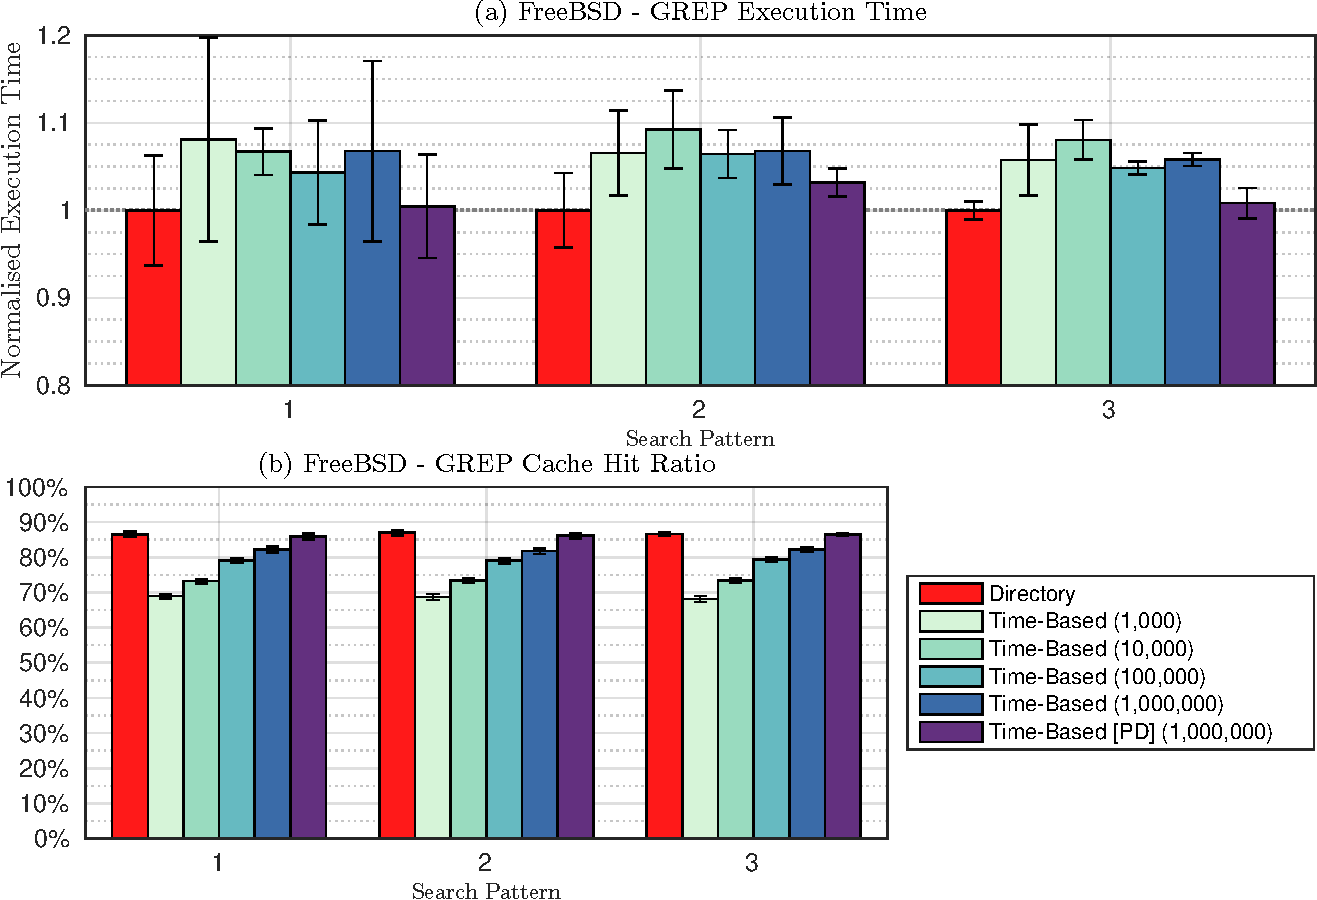
\includegraphics[width=\textwidth,height=\textheight,keepaspectratio,angle=0]{grep_freebsd_full}}
			\caption{FreeBSD GREP performance evaluation} 
			\label{grep_freebsd_full}
		\end{figure}

		The results are shown in Figure \ref{grep_freebsd_full}. The patterns are arranged in order of most frequent to least frequent. The PD model is the best performing time-based design. The execution time of all models is proportional to the individual hit ratios. The PD model achieves cache hit ratios closest to the directory, showing comparable performance. The standard deviation of the hit ratios is very low, indicating that any fluctuation in other time-based schemes is caused by OS or hardware behaviour. The variation in grep search patterns only affects the standard deviation of results and the relative performance of all coherence models is similar for every search pattern.
		

%\clearpage	
	\subsection{MD5}
		\label{results_md5}
		This widely adapted cryptographic hash function is commonly used to verify data integrity. The algorithm operates on variable sized data and generates a fixed length hash (128 bits). The input data is split into 512 bit blocks and padded when necessary. The algorithm consists of Boolean and memory operations. Time taken to produce the hash is proportional to the size of input data. Three files are used as input in this test, same as those used in the CP test.
		
		Test results are shown in Figure \ref{md5_freebsd_full}. The most performance variation is observed when hashing the smallest file size. For the time-based models (1,000 -- 100,000) the pattern is very similar, gradual execution time improvement. 
		
		\begin{figure}[!ht]
		\centering 
			\makebox{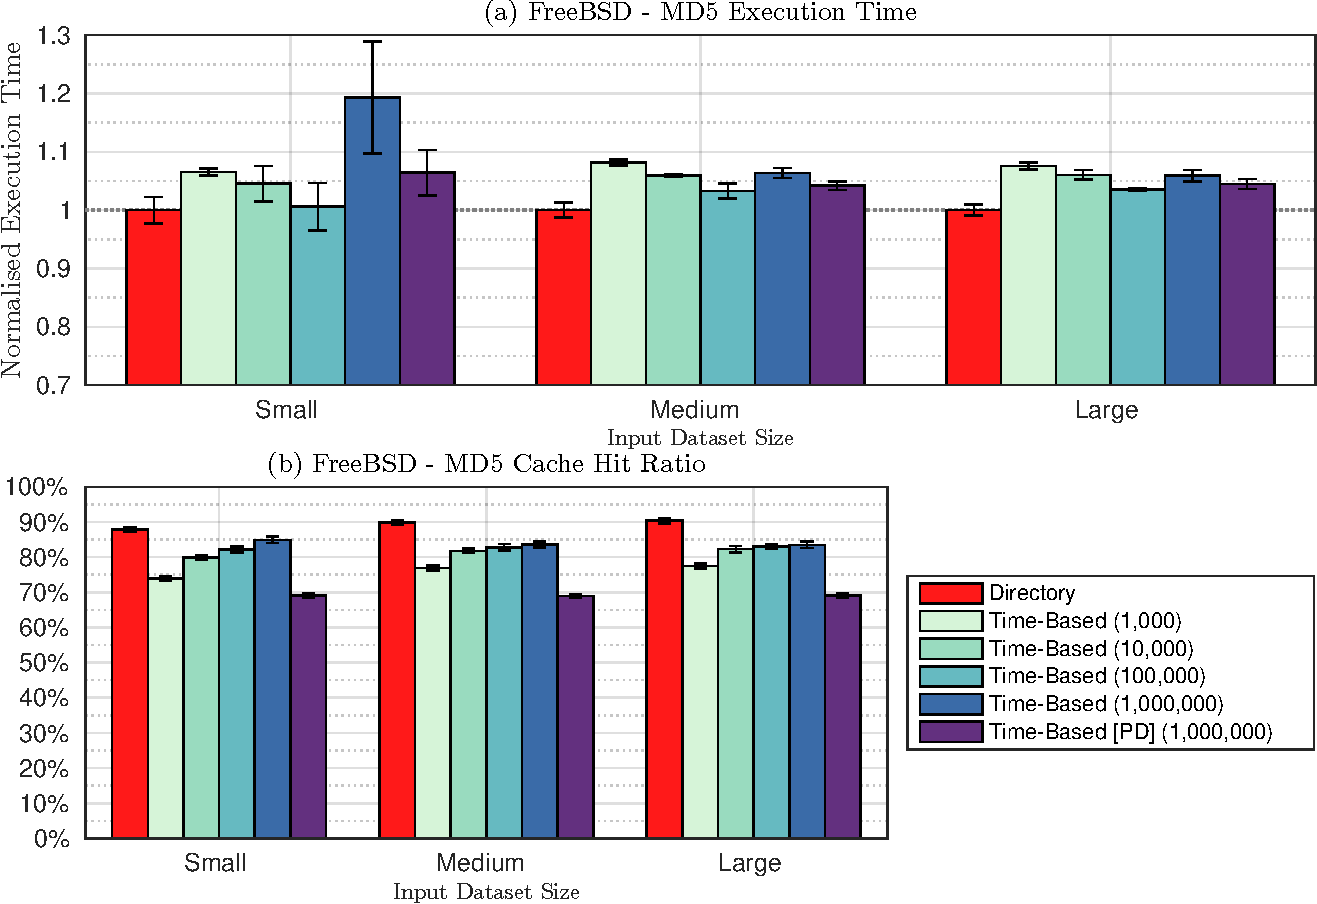
\includegraphics[width=\textwidth,height=\textheight,keepaspectratio,angle=0]{md5_freebsd_full}}
			\caption{FreeBSD MD5 performance evaluation} 
			\label{md5_freebsd_full}
		\end{figure}
		
		On an average the PD model is only second to the 100,000 model, despite showing the lowest hit rate. This indicates that some polling operations are used, and explains the sharp drop in performance from the 100,000 to 1,000,000 models. Note that polling operations are not inherent to the application itself, instead they are likely induced by the kernel when it schedules threads, services interrupts, and performs other functions.

			
%\clearpage	
	\subsection{SHA-256}
		\label{results_sha}
		This application is a common cryptographic hash function. As the name suggests, sha-256 yields 256 bit digests. The algorithm consists of Boolean and memory operations, performing multiple rounds on data blocks. Three input files are used, identical to previous tests.
		
		Test results are shown in Figure \ref{sha_freebsd_full}. In this test the PD scheme shows the weakest performance of all evaluated time-based models. The lower hit ratio of this model suggests that polling is being detected, however, the slow execution time suggests some false polling detection. The overall performance of the PD model is still within 10\% of the baseline. This test illustrates that the polling detection mechanism can be improved to limit false detection.

		\begin{figure}[!ht]
		\centering 
			\makebox{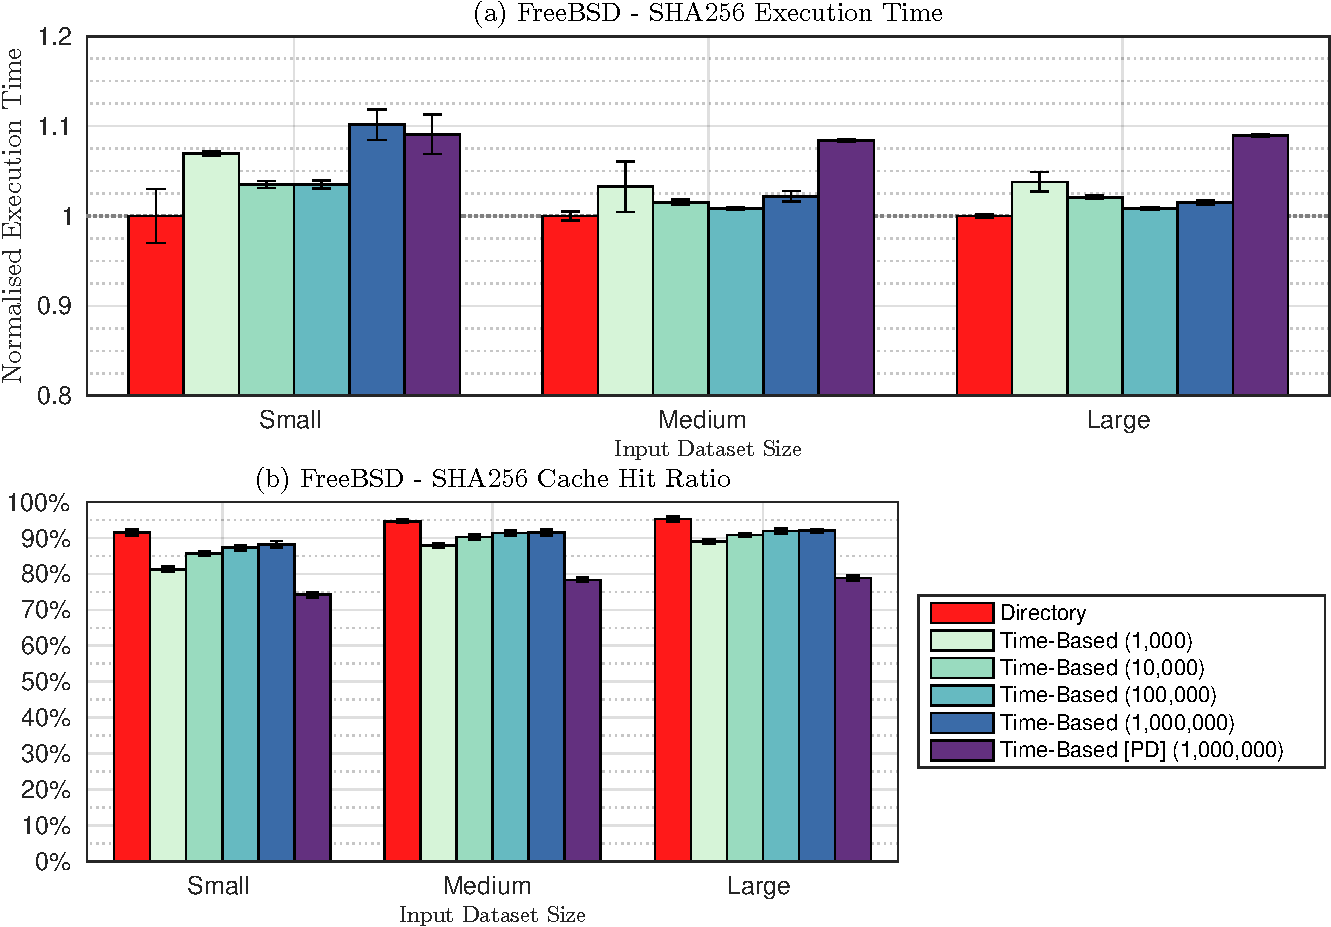
\includegraphics[width=\textwidth,height=\textheight,keepaspectratio,angle=0]{sha_freebsd_full}}
			\caption{FreeBSD SHA-256 performance evaluation} 
			\label{sha_freebsd_full}
		\end{figure}

%\clearpage
	\section{Communication Energy Estimation}
		The time-based coherence model does not require a coherence network, as a result the logic overheads are lower (elaborated in Section \ref{section_fpga_overheads}). However, results discussed in this chapter show that this coherence mechanism frequently increases the cache miss rate, generating more memory requests than the directory mechanism. 
		
		Cache statistics collected for the Splash-2 benchmarks can be used to calculate the communication overheads between the L1 and L2 caches for both coherence schemes. The bit lengths of memory requests and coherence messages is known, thus, energy can be estimated in terms of the number of bits communicated.
	
		\subsection{Parallel Execution}
			The BERI L1 data cache is non-write allocate and cache lines are only updated on load misses. The number of essential bits required for each type of memory request are listed below:
			\begin{itemize}
				\item L1 data cache fill request: physical address (physically mapped L2) + transaction ID (merge unit distinguishes between requests from different cores) + cached + linked (LL) $\Rightarrow$ \{40 + 8 + 1 + 1\} $\Rightarrow$ 50 bits.
				\item L2 fill response: data + transaction ID $\Rightarrow$ \{256 + 8\} $\Rightarrow$ 264 bits.
				\item Coherence message: subset of physical address (short tags do not require full address) + sharers list (core count relative) $\Rightarrow$ \{24 + 2\} $\Rightarrow$ 26 bits.
			\end{itemize}
			
			The energy cost of a cache miss is a sum of the fill request and fill response (50 + 264 = 314 bits) multiplied by the energy expended for transferring 1 bit. I will assume that the cost per bit is constant for BERI coherence models, as they use the same network. I will also assume that the energy cost for each bit of a coherence message is the same as that of a fill message. While the coherence network is separate, it runs in parallel to the regular memory network.
			
			\begin{description}
				\item [Directory-based coherence] In order to calculate communication energy overheads, the total number of cache read misses and coherence messages per test are counted. These two values allow us to estimate the total communication energy: total read miss cost + total coherence message cost.
				\item [Time-based coherence] The energy cost for this mechanism is simply the cost of a read miss. In this evaluation, I have used the time-based (1,000,000) model with no polling detection. The detector has been omitted as it is not integral to the coherence scheme.
			\end{description}

			The total communication between the L1 and L2 caches for the Splash-2 benchmarks previously used reveals that the energy consumption of the time-based scheme is within $\pm$1\% of the directory baseline value. Note that this result represents a combined total of all relevant communication displayed by the 11 benchmarks. The communication costs are obtained for 2 and 16 software thread test variants.
			The memory usage of each benchmark is different, hence, the total energy overhead displayed here is not representative of individual test results.
			
			The two coherence models show greater variance for individual Splash-2 benchmarks. For instance, in the FMM (Small) test, the time-based model shows a significant overhead of $\sim$16--22\%. However, when evaluated with the FMM (Large) test, the coherence model requires $\sim$2--4\% less energy than the directory. The performance of the time-based coherence improves with an increase in dataset size, thus the energy overheads are also lower.
			
			Prior evaluation has shown that the time-based model shows a weak relative performance for the Radix benchmark. The energy evaluation shows that the time-based model requires $\sim$32--50\% more energy than the directory.
			
			The time-based model does not display the best performance in the LU Contiguous benchmark, however, it shows a much better hit rate and requires 29--36\% less energy than the directory design. The directory actively communicates with all sharers, producing a better overall performance at the cost of energy overheads.
			
			These results show a large variation in communication overheads which is expected due to the diverse benchmark behaviour. The Radix benchmark manipulates local histograms and requires more fine-grained communication, which results in performance and energy overheads. The LU Contiguous benchmark is evaluated using a large block size which is much better suited to the time-based model. The FMM Small and Large tests show that for the same benchmark, significant energy and performance variations may be observed due to memory sharing patterns.
			
			The time-based model suffers overheads due to the high cost of memory fetch operations. Every fetch costs 314 bits which is approximately 12 times more than the cost of a single coherence message. The time-based model shows a good average hit ratio but it is lower than that shown by the directory. If the cost of the coherence message is increased and all other hardware parameters are unchanged, the time-based model could be more energy efficient.
			
			Note that the energy estimates presented here only focus on L1--L2 communication traffic and do not account for other variables. For instance, the directory model will expend energy through additional sharer bit lookups, coherence interface, memory controller, L1 cache coherence interface, and L1 invalidation logic. The time-based model energy expenditure will include the TTS, time-counters, and SYNC logic.
			
		\subsection{Independent Concurrent Execution}
			Multiple independent applications do not explicitly share any data, however, they do share cache space. Since cache space is limited, the applications may cause false sharing or cache thrashing. These effects are usually reduced by using associative caches. However, if the memory usage of one or both applications is high, it is likely that they will replace each other data in the caches due to cache capacity misses. 
			
			The BERI directory-based coherence mechanism is strictly inclusive and this is a disadvantage when it comes to independent applications, since the directory will need to send a coherence message to any sharer cache upon data eviction. This will result in coherence traffic and cache blocking overheads. 
			
			The time-based scheme is not influenced by shared memory evictions so it has an advantage over the directory-based scheme. The time-based model will still suffer penalties due to automatic self-invalidation and SYNC based self-invalidation, but these overheads are likely to be lower than those faced by the directory model.

		
	\section{Scalability Estimation}
		In this section I look at the current storage overheads of the BERI coherence schemes and extrapolate them to a larger number of cores.
		
		\subsection{Directory-based coherence}
			The storage overheads for this model have already been discussed in Sections \ref{dir_data_cache_structure} and \ref{dir_llc_structure}. I do not currently send any coherence messages to the L1 instruction caches so there are no overheads for these. The L1 data caches have a fixed overhead due to the short-tags optimisation, used to speed up invalidations. 
			
			In the L2 cache the directory sharers list requires one bit per cache line per L1 data cache. Thus, the directory shows a linear overhead for the sharers list. If the L1 instruction cache accesses need to be tracked then the overheads will double but would then remain constant. 
			
			The BERI caches use a fixed line capacity of 32 bytes. If you were to connect 256 L1 data caches into this L2 cache, the directory overheads per cache line would be equal to the data size (100\%). This is a highly unreasonable scenario, and beyond 4--16 cores we would expect a multiple level hierarchy such as the one outlined by Martin et al. \cite{Martin12}. The authors show that a three-level scheme can significantly improve directory overheads, less than 2\% for 256 cores. 
		
		\subsection{Time-based coherence}
			This coherence model does not add any overheads to shared memory since all of the logic is held within the L1 data caches. As with the directory design, the time-based model is not applied to the L1 instruction caches. The L1 data cache structure has been discussed in Section \ref{tts_memory_overhead}. 
			
			The tag-time-stamp adds a fixed overhead to each cache line, 4 bits in the current version. The TTS is variable and could be optimised to use smaller sizes in future versions of the coherence protocol. Darnell and Kennedy \cite{Darnell93} have previously demonstrated a timestamp based coherence mechanism which only requires 1 bit per cache line.
			
			Attaching multiple L1 data caches to a single shared memory will not add any coherence overheads to the memory infrastructure, however, larger designs would require a multi-level design, such as the one described for directory-coherence above. The time-based model implemented in the L1 caches can be extended to the L2 cache and beyond. A fixed overhead will be added to each cache line in the multiple L2's.

		
	\section{Simplicity}
		It is difficult to quantify the simplicity of a cache coherence mechanism as some estimates may be subjective. From a hardware standpoint, the simplest coherence mechanism is one that relies purely on software support, but software developers prefer a less complex model.
		
		The directory-based coherence scheme requires more infrastructure and resources as compared to the time-based model. The directory must track sharer caches and distribute coherence messages, whereas the time-based coherence scheme need not be aware of any other caches.
		
		Hardware overheads are another way of judging design complexity. I have already illustrated the FPGA overheads for both coherence schemes (Section \ref{section_fpga_overheads}), and the time-based scheme requires 1--2\% less logic. FPGA logic and area overheads are variable and HDL optimisations may change the final design outcome. I have to trust the Bluespec compiler and Quartus tools to make correct optimisations.
		
		Development time is also a factor worth considering, however, it is highly subjective. I required more time to develop the BERI directory protocol and adapt it for FreeBSD OS support, however, unanticipated hardware and OS bugs extended the development time. Whereas, the first iteration of the time-based protocol was able to boot the OS and remained stable throughout.

%\clearpage
	\section{Summary}
		The evaluation of the time-based model has shown that it is possible to approach the performance level of directory-based coherence without any explicit messaging. The polling detection optimisation significantly improves the time-based protocol. However, the directory-based coherence design is undoubtedly superior over a wide range of test variations, moreover the benefits of coherence messaging are evident. 
		
		Future improvements and optimisations of the time-based protocol could allow this scheme to surpass the performance of level of this directory-based design. The two protocols have been evaluated on a dual-core system, and a larger system behaviour is yet unknown.


% 3 lines below ensure that there is a blank page before a new chapter
\clearpage
\thispagestyle{empty}
\mbox{}
%TODO: Conclude
\makeatletter
%\newcommand{\rmnum}[1]{\romannumeral #1 }
%\newcommand{\Rmnum}[1]{\expandafter\@slowromancap\romannumeral #1@}
\makeatother
\ifpdf
\graphicspath{{Conclusion/ConclusionFigs/PNG/}{Conclusion/ConclusionFigs/PDF/}{Conclusion/ConclusionFigs/}}
\else
\graphicspath{{Conclusion/ConclusionFigs/EPS/}{Conclusion/ConclusionFigs/}}
\fi

\chapter{Conclusions and Future Research}
	In this dissertation I have presented a novel time-based cache coherence mechanism, built into the BERI multiprocessor platform.
	Hardware coherence is typically managed through shared memory or dedicated logic, however, this time-based scheme removes the need for any coherence messaging, and does not require any form of snooping or sharer tracking. Coherence is controlled directly through the private CPU caches. This top down approach reduces the need for any coherence logic, since data is updated whenever a cache line expires.
	
	Another novel aspect of this coherence model is the ability to mask local cache side-channel attacks, a feature not typically attributed to cache coherence. To the best of my knowledge, there is no other cache coherence scheme which offers explicit side-channel masking as a part of the default mechanism. However, the masking techniques displayed by this coherence scheme have been previously investigated.

	\section{Coherence}
		The work described in this dissertation is based on two cache coherence schemes that I have developed as a part of the multiprocessor extension to BERI. The BERI directory-based implementation is representative of a typical directory coherence protocol. The directory keeps track of data sharing and resides in the shared L2 cache, communicating with the private caches through a coherence network. The  protocol has been verified to support a strong memory consistency model, using a range of memory consistency checking tools. This coherence scheme in not as advanced as some directory protocols \cite{Sanchez12,Cuesta11,Cuesta13}, however, I have introduced some performance optimisations such as the L1 cache short-tags scheme. This mechanism allows parallel memory and invalidate lookups in the L1 caches, reducing overall cache blocking.
		
		The time-based cache coherence protocol is the second scheme implemented in multiprocessor BERI. Unlike other schemes based on timestamps and cache self-invalidation, this mechanism does not require any additional software support and relies on common software synchronisation techniques.
		Additionally, this time-based scheme is designed on a general purpose platform supporting a broad range of software applications together with standard OS support.

		The cache self-invalidation behaviour guarantees forward progress for memory polling operations, as stale data will eventually expire and be replaced. However, waiting for cache line time-outs is not an efficient way of updating memory, this drawback is diminished by incorporating private cache polling detection logic. This mechanism is not directly a part of the coherence model, and acts as an optimisation, similar to a memory prefetcher or other speculation logic.

		The coherence scheme enforces a relaxed memory consistency model; correctness of this design has been proven through rigorous memory consistency analysis. Relaxed memory consistency is implemented on commercial processor architectures such as ARM and PowerPC, supporting common operating systems and software. 
		
		\subsection{Performance Evaluation}
			The time-based coherence model is compared against the directory-based coherence scheme. The two protocols are compared through a range of Splash-2 benchmarks and some common FreeBSD applications. The time-based coherence scheme shows a comparable performance and occasionally outperforms the directory. 
			
			The polling detection optimisation significantly improves the corner cases where the regular time-based model suffers performance penalties. The time-based coherence scheme and the polling detection mechanism can be further improved, but it will require a much wider analysis of software applications which are not currently available on our system.
	
		\subsection{Memory Consistency}
			I have made some observations while analysing the memory consistency behaviour of BERI coherence protocols. The choice of a consistency model is usually related to legacy hardware and software; Intel processors use advanced hardware designs to enforce strict memory consistency. While this design can significantly reduce software complexity, some performance may be lost.
			
			A weak consistency model can always be strengthened through appropriate software synchronisation primitives, however, a strict model can not be weakened. The choice of a consistency model usually falls in one of two categories: (1) a strong hardware coherence model will result in higher development costs and design complexity, but simpler software design, (2)  a weak model is easier to implement in hardware, but requires strong software synchronisation support.
			
			The hardware implementation of synchronisation schemes may be open to interpretation and could lead to performance drawbacks. For instance, FreeBSD generously uses SYNC instructions to ensure a consistent memory behaviour, however, coherence designs such as the time-based scheme suffer from frequent cache invalidates. Further evidence is provided by Sung and Adve \cite{Sung15}. Relaxed consistency systems can benefit from a wider range of synchronisation primitives, MIPS lacks this support but other ISAs such as ARM have a wider selection.

	\section{Side-Channel Attacks}
		Another interesting aspect of cache coherence schemes not typically explored is the resilience to side-channel attacks. Coherence models are typically optimised to achieve maximum parallel performance. However, they are rarely, if ever used to mitigate or mask cache side-channel leakage. I demonstrate that the time-based coherence model provides some mitigation against L1 cache side-channel attacks out of the box.
		
		While the time-out aspect of this scheme provides some side-channel masking, the maximum effect is achieved whenever a critical application executes a SYNC instruction as its final operation. This achieves a full L1 single cycle flush, removing all data from that cache. The coherence scheme does not mitigate attacks at the shared memory level, but solutions to this problem are suggested in Chapter \ref{chapter_sca}.
	
	
	\section{Engineering Contributions}
		Work described in this dissertation has lead to a number of engineering contributions in the CTSRD \& MRC2 projects \cite{CTSRD,MRC2}. Major achievements have been listed below:
	
		\paragraph{The BERI multiprocessor architecture}
			\begin{enumerate}
				\item A core identification mechanism.
				\item Modifications to memory interfaces.
				\item Two major cache coherence mechanisms.
				\item Caches have been modified to accommodate the coherence schemes.
				\item Load Linked and Store Conditional instruction implementation for the multiprocessor.
				\item Testing and verification of all multiprocessor designs.
				\item Changes to the hardware synthesis procedure.
			\end{enumerate}

		\paragraph{Bringing up FreeBSD on multi-core BERI}
			\begin{enumerate}
				\item Identifying and resolving cache coherence bugs.
				\item Diagnosing incorrect OS booting behaviour.
				\item Resolving Load Linked and Store Conditional bugs in hardware.
				\item Diagnosing incorrect TLB behaviour.
				\item Identifying incorrect OS driven multiprocessor interrupts.
			\end{enumerate}	
		\paragraph{Tests created for multi-core BERI}
			\begin{enumerate}
				\item Bare metal tests for evaluating multiprocessor behaviour.
				\item A range of OS based applications used for diagnosing coherence drawbacks.
				\item Tests for evaluating the resilience of cache coherence to timing side-channel attacks (bare metal and OS).
			\end{enumerate}

	
	\section{Conclusion}
		With reference to the original hypotheses in Section \ref{hypotheses}, the following conclusions can be drawn:
	
		\begin{enumerate}
			\item The detailed evaluation in this dissertation provides compelling evidence that cache coherency is achievable without explicit coherent messaging, either hardware or software directed.  
			\item Time-based local-cache self-invalidation is indeed sufficient to support a relaxed memory consistency model. Validation has been completed through full system testing, running a selection of concurrent benchmarks, and through the AXE trace checker.
			\item Existing load-linked/store-conditional and sync instructions were demonstrably sufficient to run complex concurrent code unmodified, including the FreeBSD operating system and Splash-2 benchmarks.
			\item A detailed performance analysis was undertaken comparing the time-based coherency scheme (with and without refinements) against my implementation of a directory-based scheme. My results indicate that the refined time-based scheme is sometimes more efficient than the directory-based scheme, but often lags behind a fraction. That said, the differences were often only within a few percent, and refinements to either model are likely to nudge either model ahead of the other. Results so far are most complete for a dual-core system, and detailed analysis of large-scale multi-core systems is left as future work.
			\item Side-channel attacks on time-based coherence have been analysed.  The self-invalidation mechanism has demonstrably been shown to mitigate such attacks, particularly when the invalidation time period is reduced.  Moreover, software can make judicious use of the synchronisation instruction which flushes the cache on the time-based model, thereby reducing L1 cache side channels.
			\end{enumerate}
	
\begin{comment}
		The time-based coherence mechanism described in this dissertation is proof that cache coherence can be achieved without any explicit coherence communication. This scheme maintains global coherence by exploiting common software synchronisation techniques (barriers and locks) and by periodically auto-updating stale cached data. The coherence scheme complies with a well defined and wide used relaxed memory consistency model, which provides strong programmer assurances and software guarantees.
		
		The time-based coherence model can be competitive against a conventional directory-based coherence protocol, however, certain hardware optimisations are necessary. The absence of explicit coherence messaging reduces the hardware logic overheads of the time-based protocol, potentially reducing the coherence communication energy expenditure. However, further evaluation is necessary to verify the energy costs.
		
		The time-based coherence model can provide some mitigation against private cache side-channel attacks. It uses the software synchronisation mechanisms for cache flushing and adds entropy to memory access latency. The coherence scheme does not actively protect the last level cache, however, the cache could be adapted to use this mitigation technique.
\end{comment}
	
	\section{Future Research}
		\label{section_further_research}
		
		\subsection{Capability Enhancement of Time-Based Coherence}
			The time-based coherence model can benefit from software directed dynamic time-out selection. The time-based mechanism currently does not differentiate between shared and unshared data. Unshared data does not need to be self-invalidated, so the number of false self-invalidates can be greatly reduced if the cache can make this differentiation. 
			
			The polling detector can speculatively identify some shared memory accesses, however, it could be significantly complemented by software hints. In order to support dynamic self-invalidation, we require compiler support and a hardware mechanism to change cache settings. C11 currently supports atomic operations, used to declare shared data. The Capability approach could be used to assign time-out values to shared data. Since Capabilities specify the range of protected memory, the mechanism can be used to specify regions of shared memory. Compiler support for such instructions is currently in development and beyond the scope of this dissertation.
	
			Under the capability model implemented in CHERI, each pointer to a memory location can be compiled with the capability extension. A load or store through the pointer would result in a capability co-processor lookup, in addition to the regular TLB lookup. This mechanism protects the memory location pointed by the pointer, and prevents out-of-bound accesses to said memory. The capability pointer extension has several reserved bits that can be used for other architectural enhancements. The time-out of a memory block can be tuned depending on the nature of the process; the time-out information can be carried in the reserved bits of the capability.
			
			When a master-pointer capability is created, the time-out for the given process can be selected. Moreover, specific shared pointers can carry individually set time-outs. The master-capability contains information regarding the memory bounds. This information will be stored in the private cache of the executing core, along with the time-out specified in the capability. A combination of the two provides the cache with sufficient information as to how long the data will be held in the cache. Non-shared data could reside in the cache until evicted or explicitly invalidated, thereby improving spacial and temporal locality of a regular fixed-time-out time-based coherence protocol. 
			
			The data cache will contain a table of available time-outs, ranging from very short to infinite. A simple 2-3 bit field in the capability will dictate the time-out selection. For a C11 style atomic operation the time-out can be low, $\sim$1,000--10,000 cache cycles. For other blocks of data the time-out can be larger, $\sim$1,000,000 cache cycles or more. The data cache will hold an address-range table holding all time-out selections. When a line is loaded into the cache, the current address will be checked against the table. If the address falls within a certain range then the time-out specified will be used, otherwise a default time-out will be set. When a master-capability is loaded, the table will be populated and the time-out in the capability will be used in its tag-time-stamp. 
			
			The rest of the cache behaviour for LL/SC and SYNC instruction will remain the same. The large default time-out will continue to guarantee some progress and eliminate deadlocks.
				
		\subsection{Scalability}
			Research illustrated in this dissertation shows that a growing support for relaxed memory models can simplify cache coherence designs, while still approaching the performance levels of more sophisticated designs. Scalability analysis of the time-based scheme has been limited by FPGA capacity, but new developments may allow a more comprehensive study. The BERI core used in this research can be extended with advanced memory features and used for further relaxed memory consistency research. 
		
			This study has been limited to a dual-core evaluation, however, using a larger FPGA chip can overcome this limitation.
			An alternative approach would be a hardware based memory-only evaluation using a framework similar to AXE, but absence of non-memory operations may skew the results.
			Simulators such as GEM5 \cite{GEM5} or L3 \cite{Fox15} can also be used for larger scale testing.
		
		\subsection{Cache Configurations}
			BERI uses a simple cache design, suitable for time-based coherence testing. The coherence model could be re-evaluated on improved versions of the BERI memory system in the future.
			
		\subsection{Hardware Speculation}
			In this dissertation I have introduced the polling detection scheme as an optimisation for the time-based coherence protocol. Further hardware optimisations and speculation techniques could reduce the amount of memory communication required for this protocol, thus, leading to a more efficient and effective coherence scheme.
			
		\subsection{Side-Channel Leakage Detection}
			Side-channels can be introduced by the application code and the compiler, tools such as CacheAudit \cite{Doychev13} can be used to quantify side-channel, however, software analysis is not sufficient to prevent all attacks.
			
			To our knowledge there is no standardised way of checking side-channel leakage in hardware models, specifically caches. Researchers in this field typically develop their own prototypes for conducting leakage analysis. One hardware profiling tool is described by Ferdinand et al. \cite{Ferdinand99}. This research was first published in 1999 and an updated version would be preferable.
			
			FPGA's are frequently used for hardware prototyping. Soft-core processor models, such as the BERI processor, and memory systems can be built and evaluated on FPGA's. Hardware prototyping tools typically use verilog or similar HDL languages, so there is a potential for designing a hardware SCA testing framework. 
			
			The efforts described in Chapter \ref{chapter_sca} illustrate the benefits of testing hardware and not just evaluating software vulnerabilities. The experiments I have designed could be extended and integrated into a model checker (such as AXE), allowing the quantification of cache SCA resilience and acting as a platform for future development.
			
			%There haven't been many cache analysis tools designed specifically for hardware based cache leakage analysis, typically  done by applying the known SCAs on new hardware.  
	
			%Software such as CacheAudit \cite{Doychev13} allows a programmer to verify and analyse the potential of an application to leak side-channels information. 
			
			%However, to our knowledge there is no standardised way of checking side-channel leakage in hardware models, specifically caches. FPGA's are frequently used for hardware prototyping. Soft-core processor models, such as the BERI processor, and memory systems can be built and evaluated on FPGA's. Hardware prototyping tools typically use verilog or similar HDL languages, so there is a potential for designing a hardware SCA testing framework. The efforts described in this chapter illustrate the benefits of testing hardware and not just evaluating software vulnerabilities. The experiments I have designed could be extended and integrate into a model checker (such as AXE), allowing the quantification of cache SCA resilience and acting as a platform for future development. 



% 3 lines below ensure that there is a blank page before a new chapter
%\clearpage
%\thispagestyle{empty}
%\mbox{}

%TODO: References
%\bibliographystyle{Classes/CUEDbiblio}
%\bibliographystyle{Classes/jmb}
%\bibliographystyle{plainnat} %this works with package natbib

%\bibliographystyle{plain} % bibliography style
\bibliographystyle{unsrt}

%\bibliographystyle{apalike}
%\bibliographystyle{alpha}
\renewcommand{\bibname}{References} % changes default name Bibliography to References
\cleardoublepage
\addcontentsline{toc}{chapter}{References} %adds References to contents page 
\bibliography{References/references} % References file


\end{document}